\newcommand{\reqid}{N/A}
\newcommand{\procid}{SB1FS-COM-A-NNN}
\newcommand{\subprocid}{SB1FS-COM-A-NNN-ZZ}
\newcommand{\procname}{GS-GSE Inicialization}
\newcommand{\subprocname}{GS-GSE Inicialization}
\newcommand{\sessionID}{<session\string_ID>}


%% Otros
\newcommand{\bs}{\textbackslash}


%Test Session Folder
\newcommand{\TestSessionFolderOnPxa}{TBC}


%
\newcommand{\fmn}{GS-GSE-FM (N)}
\newcommand{\fmr}{GS-GSE-FM (R)}

% cosas auxiliares tests

\newcommand{\tmdeco}{tmdeco}
\newcommand{\xdncDir}{{\textasciitilde}/Documents/gse\_scripts/xband\_converters\_scripts/}

%-------------------------------------------------------------------------------------------------

%% Interfaces

% de RF
\newcommand{\nSBone}{TM\&TC [S-Band] (N1)}
\newcommand{\nSBtwo}{TM\&TC [S-Band] (N2)}
\newcommand{\zSBone}{TM\&TC [S-Band] (Z1)}
\newcommand{\zSBtwo}{TM\&TC [S-Band] (Z2)}
\newcommand{\nSBtc}{TM\&TC [S-Band] (TC TP)}
\newcommand{\nSBtm}{TM\&TC [S-Band] (TM TP)}
\newcommand{\nXBone}{Data [X-Band] (N1)}
\newcommand{\nXBtwo}{Data [X-Band] (N2)}
\newcommand{\nXBtp}{Data [X-Band] (TP)}

\newcommand{\tmTB}      {TM RF TestBed}
\newcommand{\tbed}      {TestBed}
\newcommand{\crtTBIP}   {192.168.75.201}
\newcommand{\hdrTBIP}   {192.168.75.202}
%-------------------------------------------------------------------------------------------------
% SBS
\newcommand{\SBM}{S-Band Matrix}
\newcommand{\SBA}{S-Band Attenuator}
\newcommand{\SBMA}{S-Band Matrix and Attenuato}
\newcommand{\supc}{S-Band Upconverter}
\newcommand{\sdnc}{S-Band Downconverter}
\newcommand{\tlt}{S-Band Test Loop Translator}
\newcommand{\sbmaSof}     {SBMA App v1.0.0}

% XBS
\newcommand{\XBMA}{X-Band Matrix and Attenuator}
\newcommand{\xbmaSof}     {XBMA App v1.0.0}
\newcommand{\xupc}{X-Band Upconverter}
\newcommand{\xdnc}{X-Band Downconverter}
\newcommand{\xupONE}{X-Band Upconverter 01}
\newcommand{\xupTWO}{X-Band Upconverter 02}
\newcommand{\xdnONEpy}{\texttt{DownConverter01-FM\_v1.0.py}}
\newcommand{\xdnTWOpy}{\texttt{DownConverter02-FM\_v1.0.py}}
\newcommand{\xuppy}{\texttt{UpConverter-FM\_v1.0.py}}

% ITS
\newcommand{\ethST}{Ethernet Switch TMTC}
\newcommand{\ethSD}{Ethernet Switch Data}

% SUS
\newcommand{\rckttRF}{Rack TMTC-RF}
\newcommand{\rckttBB}{Rack TMTC-BB}
\newcommand{\rckdtRF}{Rack Data-RF}
\newcommand{\rckdtBB}{Rack Data-BB}
\newcommand{\rckaux}{Rack Aux}
\newcommand{\rackRfTestBed} {Rack RF TestBed}


\newcommand{\thinTT}{Operator Workstation TMTC}
\newcommand{\thinDT}{Operator Workstation Data}


\newcommand{\hdrTBCfgFileDir}     {\texttt{D:\bs{}ZDS\bs{}Data\bs{}HDR\bs{}CrtxMsc\bs{}SABIA-Mar\bs{}AIT\bs{}}}
%TI
\newcommand{\ccm}{Configuration Control Manager}

% Harness
\newcommand{\datHarness}{Data BB harness}
\newcommand{\fsHarness}{Umbilical harness}

% com- equipments
\newcommand{\stx}{EWC-29 transmitter}
\newcommand{\srx}{EWC-29 receiver}
\newcommand{\xtx}{EWC-30 transmitter}


% de Software
\newcommand{\vmWebIP}    {192.168.75.101}
\newcommand{\gsWebIP}{http://\vmWebIP:7080}
\newcommand{\gswebOperatorUser}{operator-conae}
\newcommand{\gswebOperatorPass}{operator-conae}

\newcommand{\gsWebCredentials}{
    \begin{itemize}[noitemsep]
        \item URL: \gsWebIP
        \item User: \gswebOperatorUser
        \item Password: \gswebOperatorPass
    \end{itemize}}
%-------------------------------------------------------------------------------------------------

%% VMS
% VM donde se encuentra el sinter
\newcommand{\vmFC}       {GS-GSE.SBGS09 VM}
\newcommand{\vmFCIP}     {192.168.75.109}

\newcommand{\cortexQ}{Cortex CRT-Q}
\newcommand{\crtIP}{192.168.75.151}
\newcommand{\modemCfgFileDir}{\texttt{D:{\bs}ZDS{\bs}Data{\bs}CRT{\bs}MCS{\bs}SABIA-Mar{\bs}}}
\newcommand{\modemCfgFile}{\texttt{SB1GS-GSE-FM\_RF\_BB-Umbilical\_v1.2.mcs}}
\newcommand{\modemCfgRFBB}{\modemCfgFile}
\newcommand{\modemCap}{\texttt{D:{\bs}ZDS{\bs}Data{\bs}CRT{\bs}MCS{\bs}}}

\newcommand{\cortexHDR}{Cortex HDR}
\newcommand{\hdrIP}{192.168.75.161}
\newcommand{\hdrCfgFileDir}{\texttt{D:{\bs}ZDS{\bs}Data{\bs}HDR{\bs}MCS{\bs}SABIA-Mar{\bs}}}
\newcommand{\hdrCap}{\texttt{D:{\bs}ZDS{\bs}Data{\bs}HDR{\bs}MCS{\bs}}}
\newcommand{\hdrCfgN}{\texttt{SB1GS-GSE-FM-N\_RF\_v1.4.mcs}}
\newcommand{\hdrCfgROne}{\texttt{SB1GS-GSE-FM-R\_RF-N1\_v1.4.mcs}}
\newcommand{\hdrCfgRTwo}{\texttt{SB1GS-GSE-FM-R\_RF-N2\_v1.4.mcs}}

\newcommand{\versionNote}      {\textbf{Note:} version x.y is under configuration control in documents \refAD{gsen-cfg} and \refAD{gser-cfg}.}
\newcommand{\newVersionNote}   {\textbf{Note:} version x.y+1 is the new configuration generated in the previous procedure.}


\newcommand{\screen}{screenshot-000}

% VM donde se ejecutan los flujos
\newcommand{\vmTesting}  {GS-GSE.MGMT VM}
\newcommand{\vmTestingIP}{192.168.75.193}
\newcommand{\vmTestingTestFolderLocation}{/verification/}
\newcommand{\vmTestingTestFolderName}{COMM-SS-EM-FT}
\newcommand{\evidencesDir}{\texttt{/verification/\sessionID/}}


% VM donde se encuenta XBMA SW y SBMA SW
\newcommand{\vmWin}      {GS-GSE.WIN8 VM}
\newcommand{\vmWinIP}    {192.168.75.194}


% PXI computer COM-EGSE
\newcommand{\comEgse}{CEGSE}
\newcommand{\comEgseIP}{192.168.75.211}
\newcommand{\comEgseLogsLocation}{C:\string\Users\string\EGSE\ COM\string\Desktop\string\LOGs\string\ }%No quitar espacio antes de la llave final.
\newcommand{\comEgseTestFolderLocation}{C:\string\Users\string\EGSE\ COM\string\Documents\string\ }%No quitar espacio antes de la llave final.
\newcommand{\comEgseTestFolderName}{COMM-SS-FM}
\newcommand{\comEgseGui}{EGSE\_COM\_v1.0.4}

\newcommand{\pxaIP}{192.168.75.231}
\newcommand{\pxaTestFolderName}{COMM-SS-FM-PXA-config}
\newcommand{\pxaTestFolderLocation}{D:\string\Users\string\Instrument\string\Desktop}


%% copiado de latex de doc Performance
\def\result#1{\gdef\Result{#1}}
\def\status#1{\gdef\Status{#1}}
\def\extradetail#1{\gdef\Extradetail{#1}}

% #region       SectionHeaderWithReset

%% Corrientes
\newcommand{\Irx}{134 mA} %% estaba 100 , se misdio139
\newcommand{\ItxRFoff}{90 mA} %% estaba 75 , se midio 93 
\newcommand{\ItxRFon}{336 mA} %% estaba 375mA, se midioc 334
\newcommand{\Prx}{3.75 W}
\newcommand{\PtxRFoff}{2.5 W} % atr 2.8 W
\newcommand{\PtxRFon}{9.4 W} %%10.5W, se midio 9.3

\newcommand{\ItxRFoffData}{185 mA} %% medido en TF 185 , en reporte de PT se puso180
\newcommand{\ItxRFonData}{2.6 A} %% medio en TF 
\newcommand{\PtxRFoffData}{5.2 W} % medido en TF 27,9V*185mA 
\newcommand{\PtxRFonData}{70.2 W} % medido en TF 27.0V*2.6A 
\newcommand{\fileXBSend}{Data-885840\_120s\_IDLE\_VCh01\_IDLE\_sent.bin}
\newcommand{\fileXbCompare}{Data-885840\_120s\_VCh01\_payload.bin}

\newcommand{\report}[3]
{
    \result{#1}
    \status{#2}
    \extradetail{#3}
}
% #endregion

\def\rxlevel#1{\gdef\Rxlevel{#1}}
% #region       setrxlevel
\newcommand{\setrxlevel}[1]
{
    \rxlevel{#1}
}
% #endregion

\newcommand{\folder}{default}

% #region       SectionHeaderWithReset
\newcommand{\addProcedureSteps}[1]
{
    \renewcommand{\folder}{#1}
    %\immediate\openout\myfile=CheckLists/#1/README.md
    \immediate\openout\myfile=CheckLists/\folder.md
    \immediate\write\myfile{|Section|Step|Description|}
    \immediate\write\myfile{|--|--|--|}
    \input{secciones/\folder}
    \immediate\closeout\myfile
}

\newcommand{\adbox}{Ad-hoc box}
\newcommand{\tempNote}   {
\textbf{Note:} In the first power on of the day use range $T_{amb} \pm 5^{\circ}C$
}

%%%%%%%%%%%%%%%%%%%%%%%%%%%%%%%%%%%%%%%%%%%%%%%%%%%%%%%%%%%%%%%%
%% LATEX EXTRAS
%%%%%%%%%%%%%%%%%%%%%%%%%%%%%%%%%%%%%%%%%%%%%%%%%%%%%%%%%%%%%%%%

%\newcommand{\sectionseparatortextdebug}[1]{
%\multicolumn{7}{|p{\columnwidth}|}{ \cellcolor[rgb]{0,0,.6} \textcolor{white}{\bf {#1}} }\\\hline
%}

% #region       SectionHeaderWithReset
\newcommand{\SectionHeaderWithReset}[1]
{
    \stepcounter{Sec}\setcounter{Step}{0}
    \immediate\write\myfile{\theSec,\theStep,}
    \immediate\write\myfile{\theSec,\theStep,//////////////#1/////////////////}
    \sectionheader{\theSec}{#1}
}
% #endregion


\newcommand{\sectionseparatortextdebug}[1]{}

\newcommand{\notskip}{}



%%%%%%%%%%%%%%%%%%%%%%%%%%%%%%%%%%%%%%%%%%%%%%%%%%%%%%%%%%%%%%%%
%% STEPS MACROS
%%%%%%%%%%%%%%%%%%%%%%%%%%%%%%%%%%%%%%%%%%%%%%%%%%%%%%%%%%%%%%%%
% #region       SimpleExeStep
\newcommand{\SimpleExeStep}[3]
{
    \stepcounter{Step}
    %\immediate\write\myfile{\theSec,\theStep,SimpleExeStep,#1,#2,#3}
    \procedurestep{\theSec}{\theStep}{EXE}{#1}{#2}{}{}
    \stepdetail{}{}{#3}
    % \stepcounter{Step}
    % %\immediate\write\myfile{|\theSec|\theStep|#1|#2|}
    % \procedurestep{\theSec}{\theStep}{EXE}{#1}{#2}{\Result}{\Status}
    % \stepdetail{}{}{#3}
}



%new macros
\newcommand{\starSesionPXIKVM}
{
\SimpleExeStep{Start session of PXI from CEGSE KVM.}{Session started.}{  
	From CEGSE KVM, start the session of the PXI operating system using the following credentials:
    \begin{itemize}[nosep,after=\strut]
        \item User: EGSE COM    
        \item Password: Conae1234
    \end{itemize}}
}

\newcommand{\MeasureResistance}[3] % DUT, harness
{
 \SimpleExeStep{Measure electrical resistance form \textbf{#2} connector.}
 {Measured values $\approx$ Expected values.}
 {Connect the  positive red lead of the multimeter to the \textbf{P Tip} pin and 
 the negative black lead to the \textbf{N Tip} pin of BOB. Measure the resistance between 
 the \textbf{P Tip} pin and \textbf{N Tip} pin
 using the PXI multimeter as detailed in the following table. \newline

 #3
 }   
}



\newcommand{\ConnectBOBtoDut}[2]
{
    \stepcounter{Step}
    \immediate\write\myfile{\theSec,\theStep,ConnectBOB #1  to #2}
    \procedurestep{\theSec}{\theStep}{EXE}{Connect the \textbf{#1 BOB} to \textbf{#2} connector.}{\textbf{#1 BOB} connected to \textbf{#2} connector.}{}{}
    \stepdetail{1}{0}{Use the extender cable (#1 female to #1 male) to connect the \textbf{#1 BOB} to \textbf{#2} connector.}
}

\newcommand{\DisConnectBOBtoDut}[2]
{
   
\SimpleExeStep{Disconnect the \textbf{#1} box form \textbf{#2}.}
{\textbf{#1} disconnected}
{Disconnect extender cable from the \textbf{#1} and the \textbf{#2} connector}    
}



\newcommand{\ClosePXISA}
{
    \SimpleExeStep{Close PXI spectrum analyzer.}
    {PXI spectrum analyzer closed.}
    {Close \textbf{NI RFSA Soft Front Panel(64-bit)}.}
}

\newcommand{\ClosePXIM}
{
    \SimpleExeStep{Close PXI multimeter.}
    {PXI multimeter closed.}
    {Close \textbf{NI-DMM Soft Front Panel}.}
}


\newcommand{\ConfigureNtpClientInCegse}
{
    \SimpleExeStep{
        Configure the NTP client in \comEgse{}.
    }{
        \comEgse{} time Synchronized to UTC time.       
    }{
        In the \textbf{\comEgse{}}:
        \begin{minipage}[t]{\linewidth}
            \begin{itemize}[nosep,after=\strut]
                \item Click on the current date time in the bottom-right of the screen.
                \item Click on \textbf{Change date and time settings...}
                \item Go to \textbf{Internet Time} tab  and click on \textbf{Change settings...}
                \item Set server to \textbf{192.168.75.150} and check \textbf{"Synchronize with an Internet time server"} option.
                \item Perform a manual synchronization by clicking on \textbf{Update now} button.
                \item Verify that the clock was successfully synchronized.
                \item Press OK twice to close open windows.
            \end{itemize}
        \end{minipage}
    }
}




\newcommand{\InstallAndVerifyGroundOfOscilloscope}
{
    \SimpleExeStep{
        Connect the oscilloscope to the AC power socket and verify its ground connection.
    }{
        Continuity between BNC connector outer shell and facilities ground.
    }{
        \begin{minipage}[t]{\linewidth}
            \begin{itemize}[nosep,after=\strut]
                \item Plug in the AC power cord from the AC power source into the rear panel of the Oscilloscope.
                \item Verify continuity between oscilloscope ground and facilities ground by means of multimeter
            \end{itemize}
        \end{minipage}
    }
}
\newcommand{\InstallAndVerifyGroundOfPXA}
{
	\SimpleExeStep{
		Connect the PXA to the AC power socket and verify its ground connection.
	}{
		Continuity between N connector outer shell and facilities ground.
	}{
		\begin{minipage}[t]{\linewidth}
			\begin{itemize}[nosep,after=\strut]
				\item Plug in the AC power cord from the AC power source into the rear panel of the PXA.
				\item Verify continuity between N connector ground outer shell and facilities ground by means of multimeter
			\end{itemize}
		\end{minipage}
	}
}

%%%%%%%%%%%%%%%%%%%%%%%%%%%%%%%%%%%%%%%%%%%%%%%%%%%%%%%%%%%%%%%%%%%%%%%%%%%%%%%%%%%%%%%%%%%%%%
%%%%%%%%%%%%%%%%%%%%%%%%%%%%%%%%%%%%%%%%%%%%%%%%%%%%%%%%%%%%%%%%%%%%%%%%%%%%%%%%%%%%%%%%%%%%%%
% #region       ConnectPxaExternalFreqReferenceTo
\newcommand{\ConnectPxaExternalFreqReferenceTo}[3]
{
    \stepcounter{Step}
    \immediate\write\myfile{|\theSec|\theStep|ConnectPxaExternalFreqReferenceTo|}
    \procedurestep{\theSec}{\theStep}{EXE}{Connect the external frequency reference signal to the PXA.}{
\ifstrequal{#3}{PXA}{
PXA display SENSE:EXT on lower-left corner of screen.
}{
\ifstrequal{#3}{VSA}{
VSA display EXT REF on lower-rigth corner of screen.
}{
    \errmessage{expected VSA or PXA}
}
}

}{\Result}{\Status}
    \stepdetail{1}{0}{Connect the \textbf{EXT REF IN} port of the PXA to the free 10 MHz port of #1 through the  BNC male to BNC male cable #2.
        \Extradetail
    }
}
% #endregion

% #region       DisconnectPxaExternalFreqReference
\newcommand{\DisconnectPxaExternalFreqReference}[2]
{
    \stepcounter{Step}
    \immediate\write\myfile{|\theSec|\theStep|DisconnectPxaExternalFreqReference|}
    \procedurestep{\theSec}{\theStep}{EXE}{Disconnect the external frequency reference signal from the PXA.}{
\ifstrequal{#1}{PXA}{
PXA display SENSE:INT on lower-left corner of screen.
}{
\ifstrequal{#1}{VSA}{
VSA display INT REF on lower-rigth corner of screen.
}{
    \errmessage{expected VSA or PXA}
}
}
}{\Result}{\Status}
    \stepdetail{1}{0}{Disconnect the \textbf{EXT REF IN} port of the PXA.\\
        #2\Extradetail
    }
}
% #endregion

%%%%%%%%%%%%%%%%%%%%%%%%%%%%%%%%%%%%%%%%%%%%%%%%%%%%%%%%%%%%%%%%%%%%%%%%%%%%%%%%%%%%%%%%%%%%%%
%%%%%%%%%%%%%%%%%%%%%%%%%%%%%%%%%%%%%%%%%%%%%%%%%%%%%%%%%%%%%%%%%%%%%%%%%%%%%%%%%%%%%%%%%%%%%%


\newcommand{\StopXB}
{
    \SimpleExeStep{Stop DUT transmission.}
    {Transmission stopped.}
    { In the \comEgse{}{} SW:
    \begin{minipage}[t]{\linewidth}
        \begin{itemize}[nosep,after=\strut]
            \item Go to the \textbf{COMM} tab and then go to the \textbf{Downlink} sub-tab.
            \item Press \textbf{Stop} button.
            \item Verify that \textbf{TxFinished} indicator in \textbf{ON}.
        \end{itemize}
    \end{minipage}}
}

\newcommand{\SendStoredFileXBand}[2]
{
    \SimpleExeStep{
        Start data transmission
    }{
        Data transmission started
    }{
        In the \comEgse{}{} SW:
        \begin{minipage}[t]{\linewidth}
            \begin{itemize}[nosep,after=\strut]
                \item Go to the \textbf{COMM} tab and then go to the \textbf{Downlink} subtab.
                \item Verify that “stage” box does not show "Sending X-Band File" message.
                \item On the \textbf{Stored Downlink File} box choose the file \texttt{#1} in
                      \texttt{\comEgseTestFolderLocation{}\comEgseTestFolderName{}\bs{}\sessionID\bs{}\procid{}\bs{}} directory.
                \item Switch file selector to \textbf{Send Stored Downlink File}
                \item Place the switch in \textbf{#2}
                \item Switch \textbf{Bit Endianness} selector to \textbf{Big}.
                \item Press \textbf{Send} button.
                \item Verify that “stage” box shows \textbf{Sending X Band File}.
            \end{itemize}
        \end{minipage}
    }
}



\newcommand{\RdpToCortexHdrFromThinClientTTA}
{
\SimpleExeStep{\textbf{RDP connection} to  \cortexHDR{} from \thinTT A.}
{\thinTT A connected to \cortexHDR.}
{From the \thinTT A open the Remote Desktop Connection and connect to IP: \hdrIP
\begin{itemize}[nosep,after=\strut]
    \item \texttt{User: cortex}
    \item \texttt{Password: cortex}
\end{itemize}}
}
\newcommand{\RdpToCortexHdrTBFromThinClientTTA}
{
	\SimpleExeStep{\textbf{RDP connection} to \textbf{Testbed's} \cortexHDR{}  from \thinTT A.}
	{\thinTT A connected to Testbed's \cortexHDR.}
	{From the \thinTT A open the Remote Desktop Connection and connect to IP: \hdrTBIP
		\begin{itemize}[nosep,after=\strut]
			\item \texttt{User: cortex}
			\item \texttt{Password: cortex}
	\end{itemize}}
}

\newcommand{\configOSC}[1]   % en banda X : TX-RFOFF 185 mA, TX-RFON 2,6A
{
\SimpleExeStep{Configure oscilloscope}
{Oscilloscope configured}
{    
\ifstrequal{#1}{SB}
{Configure oscilloscope to measure a current range of 80 to 350 mA.}
{\ifstrequal{#1}{XB}
{Configure oscilloscope to measure a current range of 170 to 2800 mA.}}

}

}


\newcommand{\StarMultimeter}[1]
{
\SimpleExeStep{Configure PXI multimeter}
{PXI Multimeter configured}
{    \begin{itemize}[nosep,after=\strut]
    \item Start PXI multimeter by clicking on the
         \textbf{NI-DMM Soft Front Panel} icon on the desktop.
    \item Set the PXI multimeter to measure \textbf{#1}.
   \end{itemize}
 
}    
}

\newcommand{\StartPXISpectrumA}
{
\SimpleExeStep{Start PXI spectrum analyzer.}
{PXI spectrum analyzer started.}
{Start PXI spectrum analyzer by clicking on the
\textbf{NI RFSA Soft Front Panel(64-bit)} icon on the desktop.}

}

\newcommand{\configPXISpectrumA}[2]
{
\SimpleExeStep{Configure PXI spectrum analyzer.}
{PXI spectrum analyzer configured.}
{
    \begin{itemize}[nosep,after=\strut] 
    \item Load the configuration 
    file from the \texttt{C:/USERS/EGSE COM/Documents/
    COMM-SS-FM/\sessionID/\procid/NI-RFSA-data-config} directory.
      \begin{itemize}
      	\item \textbf{#1}
      	\item \textbf{#2}
      \end{itemize} 
    
    \item Select the external reference: \textbf{Device/System}
     -> \textbf{Freq Ref Scr} -> \textbf{Ref In}
    \end{itemize}
}
 }



\newcommand{\VerifyRxSpeLevel}
{
\SimpleExeStep{On \comEgse{} GUI verify O\_RX\_SPE\_LEVEL value.}
{$value \approx 2.4 V$}
{ On \comEgse{} GUI got to ASM tab to read \textbf{O\_RX\_SPE\_LEVEL}. 
Verify that read value meets expected value.\newline
\textbf{Note:} Expected TM value corresponding to frequency shift of 0 Hz. See \refAD{ewc29-icd}}    
}
\newcommand{\VerifyRxAgcLevel}
{
\SimpleExeStep{On \comEgse{} GUI verify O\_RX\_AGC\_LEVEL value.}
{$value \approx {1.93} V$}
{ On \comEgse{} GUI got to ASM tab to read \textbf{O\_RX\_AGC\_LEVEL}. Verify that read value meets expected value.\newline
\textbf{Note:} Expected TM value corresponding to RX power of {-91} dBm. %See \refAD{ewc29-icd}
}    
}


\newcommand{\DisconnectExternalReferenceSignalToPXISB}
{
\SimpleExeStep{Disconnect the external reference signal from PXI and \gse.}
{Reference signal disconnected.}
{
    \begin{itemize}[nosep,after=\strut]
        \item Disconnect cable SBB4.18 from the \textbf{REF IN} port of the NI PXIe-5653 module.
        \item Disconnect other end of cable SBB4.18 from Power Splitter 
        TMTC port.
    \end{itemize}
    \textbf{Note}: If SB1FS-COM-F-003 test is carried out next, skip this step.
}    
}


\newcommand{\DisconnectExternalReferenceSignalToPXIXB}
{
\SimpleExeStep{Disconnect the external reference signal from PXI and \gse.}
{Reference signal disconnected.}
{
    \begin{itemize}[nosep,after=\strut]
        \item Disconnect cable SBB4.18 from the \textbf{REF IN} port of the NI PXIe-5653 module.
        \item Disconnect other end of cable SBB4.18 from Power Splitter 
        Data port.
    \end{itemize}
}    
}

\newcommand{\ConnectExternalReferenceSignalToPXI}
{
\SimpleExeStep{Connect the external reference signal to the PXI.}
{PXI connected to the reference signal.}
{Connect the \textbf{REF IN} port of the NI PXIe-5653 module to the free port of the Power Splitter 
DATA \gse-FM (R) through the  BNC male to SMA male cable SBB4.18.}    
}



\newcommand{\VerifyTxStatusSBand}[1]
{
\SimpleExeStep{Check Tx status}{
\ifstrequal{#1}{Standby}{
    \textbf{Standby Mode} indicator is ON
}{
    \ifstrequal{#1}{Pure Carrier}{
        \textbf{Pure Carrier Mode} indicator is ON
    }{
        \ifstrequal{#1}{Modulation}{
            \textbf{Modulation Mode} indicator is ON
        }{
            \errmessage{Unexpected mode}
        }
    }
}}
{Verify Tx Status in \textbf{STATE} section of \comEgse{} GUI.}
}

\newcommand{\VerifyTxStatusXBand}[1]
{
\SimpleExeStep{Check Tx status}{
\ifstrequal{#1}{Standby}{
    \textbf{Standby Mode} indicator is ON
}{
    \ifstrequal{#1}{Modulation}{
        \textbf{Operation Mode} indicator is ON
    }{
        
            \errmessage{Unexpected mode}
        
    }
}}
{Verify Tx Status in \textbf{STATE} section of \comEgse{} GUI.}
}

%verificacion de ausencia de portadpra
\newcommand{\VerifyAbsentOfCarrierInPxi}
{
    
\SimpleExeStep{Verify absence of carrier on PXI.}
{Carrier absent on PXI.}
{Go to \textbf{NI RFSA Soft Front Panel} and verify absence of carrier on the screen.}
}
% #endregion


\newcommand{\DisconnectProbeCurrent}
{
\SimpleExeStep{Disconnect the current and voltage probes.}
{Probes disconnected.}
{Disconnect the current and voltage probes from Ad-hoc box measurement ports.}    
}


 
% cotrolar cantida de tramas en cortex
\newcommand{\CheckContCortexCRT}
{
\SimpleExeStep{Check the amount TM frames received in \cortexQ.}
{TM frames received from 2520 to 2640.}
{On the Cortex MCS (\crtIP) do the following:
\begin{itemize}[nosep,after=\strut]
    \item Go to Quick Look tab.
    \item Verify that \textbf{Counter} field has a value as expected.
    \item Press Disable button and close TMU-B. window.	 	
\end{itemize}}    
}

% Configuracion de anlizador de PXI
\newcommand{\ConfigPowerBandPXI}[1]
{
\SimpleExeStep{Configure band power measurement in PXI spectrum analyzer.}
{PXI spectrum analyzer configured.}
{Go to \textbf{NI RFSA Soft Fron Panel} and do the following:
\begin{itemize}[nosep,after=\strut]
\item Click on \textbf{Meas}, \textbf{Channel Power} and 
enter #1 in \textbf{Bandwidth} field. 
\item Click \textbf{Meas,} \textbf{Channel Power} and 
enter 100 in \textbf{Number of Averages} field.  
\end{itemize}
}    
}

% Configuracion de anlizador de PXI
\newcommand{\ConfigBandWidthPXI}
{
	\SimpleExeStep{Configure Occupied Bandwidth measurement in PXI spectrum analyzer.}
	{PXI spectrum analyzer configured.}
	{Go to \textbf{NI RFSA Soft Front Panel} and do the following:
		\begin{itemize}[nosep,after=\strut]
			\item Click on \textbf{Meas}, \textbf{Occupied Bandwidth} and 
			enter 99\% in \textbf{OBW Power} field. 
			\item Click \textbf{Meas,} \textbf{Occupied Bandwidth} and 
			enter 100 in \textbf{Number of Averages} field.  
		\end{itemize}
	}    
}




% inicio de flujo 
\newcommand{\StartTMTCRFFlow}
{
\SimpleExeStep{Start TMTC RF flow on \gse-FM}
{TMTC RF flow started.}
{From SABIA-Mar Ground Segment web, click the \textbf{Status Monitor} icon,
 in the open tab do the following:
\begin{itemize}[nosep,after=\strut]
    \item Click on the button on the left and select \textbf{New Activity}.
    \item In the displayed window, click on the icon corresponding to
     \textbf{tmtc-rf}.
    \item Enter 1800 and then click on the \textbf{Confirm} button. 
    \item Click on the \textbf{Instant} button and then click on 
    the \textbf{Confirm} bottom.
    \item Click on the \textbf{Ok} bottom.    
    \item Finally verify in \textbf{Timeline View} that \textbf{TMTC RF flow} has started.
\end{itemize}}    
}% inicio de flujo  DATA
\newcommand{\StartDataRFFlow}[1]
{
\SimpleExeStep{Start DATA RF flow on \gse-FM (R)}
{DATA RF flow started.}
{From SABIA-Mar Ground Segment web, click the \textbf{Status Monitor} icon,
 in the open tab do the following:
\begin{itemize}[nosep,after=\strut]
    \item Click on the button on the left and select \textbf{New Activity}.
    \item In the displayed window
    \begin{itemize}
        \item Click on the icon corresponding to \textbf{data-rf-n1} if \textbf{EWC30-FM1} is under test.
        \item Click on the icon corresponding to \textbf{data-rf-n2} if \textbf{EWC30-FM2} is under test.
    \end{itemize}
    
    \item Enter #1 and then click on the \textbf{Confirm} button. 
    \item Click on the \textbf{Instant} button and then click on 
    the \textbf{Confirm} button.
    \item Click on the \textbf{Ok} button.    
    \item Finally verify in \textbf{Timeline View} that \textbf{DATA RF flow} has started.

\end{itemize}}    
}





\newcommand{\OpenWinCortexCRT}
{
\SimpleExeStep{Open \textbf{Vector} and \textbf{Quick Look} tabs in Cortex CRT.}
{Tabs open.}
{Go to MCS Cortex (\crtIP), in the \textbf{Global} window, do the following:
\begin{itemize}[nosep,after=\strut]
    \item Open Vector tab.
    \begin{itemize}[nosep,after=\strut]
        \item Click in \textbf{TMU-B} (Telemetry Unit B).
        \item In the displayed window go to vector tab, select cumulative
         option and press enable button
    \end{itemize}
    \item Open Quick Look
    \begin{itemize}[nosep,after=\strut]
        \item Click in \textbf{TMU-B} (Telemetry Unit B).
        \item In the displayed window go to Quick Look tab and press enable button.
    \end{itemize}  
\end{itemize}
}    
}

\newcommand{\OpenWinCortexHDR}
{
\SimpleExeStep{Open \textbf{Vector}, \textbf{Spectrum} and \textbf{Recording Global} tabs  in Cortex HDR.}
{Tabs open.}
{Go to MCS Cortex (\hdrIP), in the \textbf{Global} window, do the following:
\begin{itemize}[nosep,after=\strut]
    \item Open Vector tab.
    \begin{itemize}[nosep,after=\strut]
        \item Click in \textbf{DMU-1} (Demodulator Unit 1).
        \item In the displayed window go to vector tab, select cumulative
         option and press enable button
    \end{itemize}
    \item Open Spectrum
    \begin{itemize}[nosep,after=\strut]
        \item Click in \textbf{DMU-1} (Demodulator Unit 1).
        \item In the displayed window go to Spectrum tab and press enable button.
    \end{itemize}  
    \item Open Recording Global
    \begin{itemize}[nosep,after=\strut]
        \item Click in \textbf{DRU-1} (Data Recording Unit 1).
        \item In the displayed window go to Recording Global tab.
    \end{itemize}  

\end{itemize}
}    
}
\newcommand{\CheckLookCortexHDR}
{
    \SimpleExeStep{Verify locked status in Cortex HDR}
    {PLL, B/S, Viterbi and F/S are locked and
    stable.}
    {
        Go to Cortex MCS (192.168.75.161) of GS-GSE-FM (R)
         do the following: 
\begin{itemize}[nosep,after=\strut]
    \item From Recording Global tab of \textbf{DRU-1} (Data Recording Unit 1)   
    \begin{itemize}[nosep,after=\strut]
        \item Verify that \textbf{PLL} is locked.
        \item Verify that \textbf{B/S} is locked.
        \item Verify that \textbf{F/S} is locked.
    \end{itemize}
    \item From Vector or Spectrum tab of \textbf{DMU-1} (Demodulator Unit 1)    
    \begin{itemize}[nosep,after=\strut]
        \item Verify that \textbf{Viterbi} is Locked.
    \end{itemize}
\end{itemize}

    Verify for 15 seconds that none of them unlock.
    }

}

% captura
\newcommand{\TakeScreenShotOnPxi}
{
\SimpleExeStep{Take screenshot of signals measurements.}
{\texttt{<filename.png>} saved.}
{ Take screenshot (use paint) and save it in 
\texttt{C:/USERS/EGSE COM/Documents/
COMM-SS-FM-FT/\sessionID/\procid/\subprocid/screenshot-pxi{}} directory
}    
}


%
\newcommand{\ptcgse}{$P_{out} = -30dBm\pm1dB.$} % potencia esperada a la salida del GSE
\newcommand{\MeasureCarrierPowerAndFreqUsingPxi}[3]
{
\SimpleExeStep{Measure carrier power and frequency.}
{$P_{out} = #1dBm\pm#2dB.$ \\ $F_{out} = #3 \ MHz.$ \\}
{Press the \textbf{Peak Search} button in \textbf{NI RFSA Soft Front Panel} and verify that the 
measured power and frequency meet the expected values.}    
}

\newcommand{\VerifyCarrierPowerAndFreqUsingPxi}[2]
{
\SimpleExeStep{Verify carrier power and frequency.}
{$P_{out} \approx #1dBm.$ \\ $F_{out} \approx #2 \ MHz.$ \\}
{Press the \textbf{Peak Search} button in \textbf{NI RFSA Soft Front Panel} and verify that the 
measured power and frequency meet the expected values.}    
}




\newcommand{\MeasureCarrierPowerModUsingPxi}[2]
{
\SimpleExeStep{Measure modulated power.}
{$P_{out} = #1dBm\pm#2dB.$}
{
Go to \textbf{NI RFSA Soft Front Panel} and do following:
\begin{itemize}[nosep,after=\strut]
    \item Wait until Avgs = 100/100 
    \item See \textbf{Measurement: Channel Power} and 
    verify that the measured meet the expected value.
\end{itemize} 
}    
}

\newcommand{\MeasureOccupiedBandwidthUsingPxi}[1]
{
\SimpleExeStep{Measure Occupied Bandwidth at 99\%.}
{$OBW_{99\%} \approx #1\ MHz$}
{Go to \textbf{NI RFSA Soft Front Panel} and do following:
\begin{itemize}[nosep,after=\strut]
    \item Wait until Avgs = 100/100 
    \item See \textbf{Measurement: Occupied Bandwidth} and 
    verify that the measured meet the expected value.
\end{itemize} }    
}

\newcommand{\MeasureLOLeakageUsingPxi}
{
\SimpleExeStep{Verify LO leakage frequency.}
{$\approx$ 8106\ MHz for \textbf{EWC30-FM1}\\ $\approx$ 8269\ MHz for \textbf{EWC30-FM2}}
{Go to \textbf{NI RFSA Soft Front Panel} and do following:
\begin{itemize}[nosep,after=\strut]
    \item Click on \textbf{Meas}, then on \textbf{All Meas Off}
    \item Click on \textbf{BW}, then on \textbf{FFT Windows}
    \item Select \textbf{FFT flat top}
    \item Press the \textbf{Peak Search} button 
    \item Wait until Avgs = 100/100 
    \item See in window the \textbf{frequency} and 
    verify that the measured meet the expected value.
\end{itemize} }    
}


% #region    
\newcommand{\MeasureVoltage}[1]
{
\SimpleExeStep{Measure voltage.}
{$V \approx 28 V$}{
    \begin{itemize}[nosep,after=\strut]
        \item Connect probes hook (+) and (-) of PXI multimeter to Ad-hoc box \textbf{#1} voltage ports.
        \item Measure voltage with PXI multimeter.
    \end{itemize}
    }    
}
\newcommand{\MeasureCurrent}[2]
{
\SimpleExeStep{Measure current.}
{$I \approx #1$}{
    \begin{itemize}[nosep,after=\strut]
        \item Connect probe current of oscilloscope to Ad-hoc box \textbf{#2} current loop.
        \item Measure current with oscilloscope.
    \end{itemize}    

}    
}


\newcommand{\ConnectToMultimeter}[1]
{
\SimpleExeStep{Connect PXI multimeter \textbf{#1}.}
{\textbf{#1} connected to PXI multimeter.}
{

Connect \textbf{#1} to the \textbf{INPUT V} ports of the 
NI PXIe-4072. Take into account the polarity.}
}
\newcommand{\DisConnectToMultimeter}[1]
{
\SimpleExeStep{Disconnect \textbf{#1} from PXI multimeter.}
{Probes disconnected form PXI multimeter.}
{

Disconnect \textbf{#1} from the \textbf{INPUT V} ports of the 
NI PXIe-4072.}
}



\newcommand{\MeasureVoltSource}
{
\SimpleExeStep{Measure COM-EGSE power supply output voltage.}{$Voltage\approx 28\ V$}
{Set the multimeter to measure voltage and measure the voltage present on the rear terminals of the COM-EGSE power supply.}
}



\newcommand{\VerifyBBConectionSB}
{
    \SimpleExeStep{
        Verify BB harness connections.
    }{
        BB harness conected.
    }{
        Verify BB harness connections between Ad-hox box and PXI. 
 
    }
}
\newcommand{\VerifyBBConectionXB}
{
    \SimpleExeStep{
        Verify BB harness connections.
    }{
        BB harness conected.
    }{
        Verify BB harness connections between Ad-hox box and PXI match the EWC30 configuration. 
 
    }
}



% #region       BdmAliveness
\newcommand{\BdmAliveness}[4]
{
    \stepcounter{Step}
    \immediate\write\myfile{\theSec,\theStep,BdmAliveness,#1,#2,#3,#4}
    \procedurestep{\theSec}{\theStep}{EXE}{BDM #4 interface input resistance measurement.}{$3 M\Omega < R < 30M\Omega$}{}{}
    \stepdetail{1}{0}{
        Set the multimeter to measure resistance.\\
        Connect the multimeter probes to pins \textbf{#1(+)} and \textbf{#2(-)} of the \textbf{#3 BOB}.}
}
% #endregion
% #region       ChangeTxStatusTo{status}{hvhpc command}
\newcommand{\ChangeTxStatusTo}[2]
{
    \stepcounter{Step}
    \immediate\write\myfile{\theSec,\theStep,ChangeTxStatusTo,CMD=#2 STATUS=#1}
    \procedurestep{\theSec}{\theStep}{EXE}
    {Send command #2 to change Tx status to #1}{command sent}{}{}
    \stepdetail{1}{0}{
        Go to HV-HPC tab on \comEgse{} GUI and press \textbf{#2} button. Button turns green during 0.6 seconds.
    }
}
% #region       CheckHardDiskSpaceOnPxi

% #endregion
% % #region       CheckHardDiskSpaceOnPxi
\newcommand{\CheckHardDiskSpaceOnPxi}
{
    \stepcounter{Step}
    \immediate\write\myfile{\theSec,\theStep,CheckHardDiskSpaceOnPxi,Free space > 65 GB}
    \procedurestep{\theSec}{\theStep}{EXE}
    {Check hard disk space on \comEgse}{free space > 8 GB}{}{}
    \stepdetail{1}{0}{
        \begin{itemize}
            \item Launch the File Explorer.
            \item In the navigation panel on the left side of the folder, click "Computer."
            \item Check available storage space displayed under WINDOWS(C) drive.
        \end{itemize}
    }
}
% % #endregion

% #region       CheckThatTMFramesAreNotRxOnTei
\newcommand{\CheckThatTMFramesAreNotRxOnTei}
{
    \stepcounter{Step}
    \immediate\write\myfile{\theSec,\theStep,CheckThatTMFramesAreNotRxOnTei}
    \procedurestep{\theSec}{\theStep}{EXE}{Check that TM frames are not being received.}{Received TM frames counters are fixed.}{}{}
    \stepdetail{1}{0}{On the web browser go to \textbf{TM\&TC Extension} tab, see \textbf{TEI-TM-VC01}, \textbf{TEI-TM-VC02} and \textbf{TEI-TM-VC63} fields and verify that received TM frames counters, \textbf{tmConaeFramesReceived}, are fixed.
        \\~\\ Note: This takes approximately 10 minutes from when the procedure script was run.
    }
}
% #endregion

% #region       CheckTheAmountOfVCFramesOnTei{VC01|V02|VC63}{2400}
\newcommand{\CheckTheAmountOfVCFramesOnTei}[2]
{
    \stepcounter{Step}
    \immediate\write\myfile{\theSec,\theStep,CheckTheAmountOfVCFramesOnTei,#1,#2}
    \procedurestep{\theSec}{\theStep}{EXE}{Check the amount TM frames received for #1.}
    {TM frames received for #1 \ifstrequal{#1}{VC63}{$\approx$}{=} #2}{}{}
    \stepdetail{1}{0}
    {
        On the web browser go to \textbf{TM\&TC Extension} tab, see \textbf{TEI-TM-#1} field and verify that received
        TM frames counter, \textbf{tmConaeFramesReceived}, has a value as expected.
    }
}
% #endregion

% #region       CheckTheAmountOfTMFramesRxOnCortex{2400}{2500}
\newcommand{\CheckTheAmountOfTMFramesRxOnCortex}[2]
{
    \stepcounter{Step}
    \immediate\write\myfile{\theSec,\theStep,CheckTheAmountOfTMFramesRxOnCortex,#1,#2}
    \procedurestep{\theSec}{\theStep}{EXE}{Check the amount TM frames received in \cortexQ.}{TM frames received between #1 to #2.}{}{}
    \stepdetail{1}{0}{On the Cortex MCS (\crtIP) do the following:
        \begin{itemize}[nosep,after=\strut]
            \item Go to Quick Look tab.
            \item Verify that \textbf{Counter} field has a value as expected.
            \item Press Disable button and close TMU-B. window.
        \end{itemize}
    }
}
% #endregion


% #region       DisableModulationOnCortex
\newcommand{\DisableModulationOnCortex}
{
    \stepcounter{Step}
    \immediate\write\myfile{\theSec,\theStep,DisableModulationOnCortex}
    \procedurestep{\theSec}{\theStep}{EXE}{Disable modulation in \cortexQ.}{Modulacion disabled. Pure Carrier.}{}{}
    \stepdetail{1}{0}{On the Cortex MCS (\crtIP) do the following:
        \begin{itemize}[nosep,after=\strut]
            \item Open IF modulator.
            \item Press Config button.
            \item Discheck modulation box.
            \item Press Apply button.
        \end{itemize}
    }
}
% #endregion

% #region       EnableModulationOnCortex
\newcommand{\EnableModulationOnCortex}
{
    \stepcounter{Step}
    \immediate\write\myfile{\theSec,\theStep,EnableModulationOnCortex}
    \procedurestep{\theSec}{\theStep}{EXE}{Enable modulation in \cortexQ.}{Modulacion enabled.}{}{}
    \stepdetail{1}{0}{On the Cortex MCS (\crtIP) do the following:
        \begin{itemize}[nosep,after=\strut]
            \item Open IF modulator.
            \item Press Config button.
            \item Check modulation box.
            \item Press Apply button.
        \end{itemize}
    }
}
% #endregion


% #region       AdjustRfOutPowerOfCortex
\newcommand{\AdjustRfOutPowerOfCortex}
{
    \stepcounter{Step}
    \immediate\write\myfile{\theSec,\theStep,AdjustRfOutPowerOfCortex}
    \procedurestep{\theSec}{\theStep}{EXE}{Adjust RF output power in \cortexQ.}{Power of -45,9dBm is measured in PXA}{}{}
    \stepdetail{1}{0}{On the Cortex MCS (\crtIP) do the following to set the output power:
        \begin{itemize}[nosep,after=\strut]
            \item Open IF modulator.
            \item Press Config button.
            \item Set Carrier Level
            \item Press Apply button.
        \end{itemize}
        Register Carrier Level final value.
    }
}
% #endregion

% #region       ConnectBOB{DB-X}{Jnnn}
\newcommand{\ConnectBOB}[2]
{
    \stepcounter{Step}
    \immediate\write\myfile{\theSec,\theStep,ConnectBOB #1  to #2}
    \procedurestep{\theSec}{\theStep}{EXE}{Connect the \textbf{#1 BOB} box to connector \textbf{#2} of the AD-HOC box.}{\textbf{#1 BOB} connected to Ad-Hoc box}{}{}
    \stepdetail{1}{0}{Use the extender cable to connect the \textbf{#1 BOB} to the \textbf{#2} input.}
}
% #endregion


% #region       ConnectAttenuatorsInNoneGsGSE
\newcommand{\ConnectAttenuatorsInNoneGsGSE}
{
    \stepcounter{Step}
    \immediate\write\myfile{\theSec,\theStep,ConnectAttenuators}
    \procedurestep{\theSec}{\theStep}{EXE}
    {Connection of 30dB Fixed Attenuators to \gse{} \nSBone interface}{Attenuation of 30 dB added in \nSBone interface}{}{}
    \stepdetail{1}{0}{
        \begin{itemize}
            \item Disconnect the 50 ohm load from \nSBone interface.
            \item Connect the 20dB Fixed Attenuator PE7015-20 (ATT18.01) to \nSBone interface.
            \item Connect the 10dB Fixed Attenuator PE7015-10 (ATT19.01) to PE7015-20 (ATT18.01).
        \end{itemize}
    }
}
% #endregion
 
% #region       ConnectAttenuatorsInNoneGsGSEXBand
\newcommand{\ConnectAttenuatorsInNoneGsGSEXBand}
{
    \stepcounter{Step}
    \immediate\write\myfile{\theSec,\theStep,ConnectAttenuators}
    \procedurestep{\theSec}{\theStep}{EXE}
    {Connection of 30dB Fixed Attenuators to \gse{} \nXBone interface}{Attenuation of 30 dB added in \nXBone interface}{}{}
    \stepdetail{1}{0}{
        \begin{itemize}
            \item Disconnect the 50 ohm load from \nXBone interface.
            \item Connect the 20dB Fixed Attenuator PE7015-20 (ATT18.01) to \nXBone interface.
            \item Connect the 10dB Fixed Attenuator PE7015-10 (ATT19.01) to PE7015-20 (ATT18.01).
        \end{itemize}
    }
}
% #endregion

% #region       DisconnectAttenuatorsInNoneGsGSE
\newcommand{\DisconnectAttenuatorsInNoneGsGSE}
{
    \stepcounter{Step}
    \immediate\write\myfile{\theSec,\theStep,DisconnectAttenuatorsInNoneGsGSE}
    \procedurestep{\theSec}{\theStep}{EXE}
    {Disconnection of 30dB Fixed Attenuators}{Attenuation of 30 dB removed from GS-GSE \nSBone interface}{}{}
    \stepdetail{1}{0}{
        \begin{itemize}
            \item Disconnect the 10dB Fixed Attenuator PE7015-10 (ATT19.01) from PE7015-20.
            \item Disconnect the 20dB Fixed Attenuator PE7015-20 (ATT18.01) from \nSBone interface.
            \item Connect the 50 ohm load to \nSBone interface.
        \end{itemize}
    }
}
% #endregion
 
% #region       DisconnectAttenuatorsInNoneGsGSEXBand
\newcommand{\DisconnectAttenuatorsInNoneGsGSEXBand}
{
    \stepcounter{Step}
    \immediate\write\myfile{\theSec,\theStep,DisconnectAttenuatorsInNoneGsGSEXBand}
    \procedurestep{\theSec}{\theStep}{EXE}
    {Disconnection of 30dB Fixed Attenuators}{Attenuation of 30 dB removed from GS-GSE \nXBone interface}{}{}
    \stepdetail{1}{0}{
        \begin{itemize}
            \item Disconnect the 10dB Fixed Attenuator PE7015-10 (ATT19.01) from PE7015-20.
            \item Disconnect the 20dB Fixed Attenuator PE7015-20 (ATT18.01) from \nXBone interface.
            \item Connect the 50 ohm load to \nXBone interface.
        \end{itemize}
    }
}
% #endregion

% #region       ConnectSDBLLoops{cable id}
\newcommand{\ConnectSDBLLoops}[1]
{
    \stepcounter{Step}
    \immediate\write\myfile{\theSec,\theStep,ConnectSDBLLoops, CABLE-ID:#1}
    \procedurestep{\theSec}{\theStep}{EXE}{Connect SBDL test loop cable #1 to Ad-Hoc box }{SBDL test loop cable #1 connected}{}{}
    \stepdetail{1}{0}{Connect SBDL test loop cable #1 between \textbf{J202} (DB-37) and \textbf{J203A} (DB-50) connectors of the Ad-Hoc box.\newline
        Tables C.3.0-1 and C.3.0-2 detail loops connections.}
}
% #endregion





% #region       ConnectMeasurementProbesToOscilloscope
\newcommand{\ConnectMeasurementProbesToOscilloscope}
{
    \stepcounter{Step}
    \immediate\write\myfile{\theSec,\theStep,ConnectMeasurementProbesToOscilloscope}
    \immediate\write\myfile{\theSec,\theStep,ConnectMeasurementProbesToOscilloscope}
    \procedurestep{\theSec}{\theStep}{EXE}{Connect measurement probe to the oscilloscope }{Probe connected according to detail.}{}{}
    \stepdetail{1}{0}{In CH1 connect current probe.\\
    \textbf{Note:} Demagnetize current probe when necessary.
    }
}
% #endregion

% #region       ConnectMeasurementProbesToOscilloscopeForXBand
\newcommand{\ConnectMeasurementProbesToOscilloscopeForXBand}
{
    \stepcounter{Step}
    \immediate\write\myfile{\theSec,\theStep,ConnectMeasurementProbesToOscilloscopeForXBand}
    \procedurestep{\theSec}{\theStep}{EXE}{Connect measurement probes to the oscilloscope }{Probes connected according to detail.}{}{}
    \stepdetail{1}{0}{In CH1 connect current probe, in CH2 connect differential probe.\\
    }
}
% #endregion


% #region       ConnectMeasurementProbesToAdHocBox
\newcommand{\ConnectMeasurementProbesToAdHocBox}
{
    \stepcounter{Step}
    \immediate\write\myfile{\theSec,\theStep,ConnectMeasurementProbesToAdHocBox}
    \procedurestep{\theSec}{\theStep}{EXE}{Connect measurement probes to the AD-HOC box }{Probes connected according to detail.}{}{}
    \stepdetail{1}{0}{
        \begin{itemize}
            \item Connect CH1 Current probe to measure TX part.
            \item Connect CH3 Current probe to measuse RX part.
            \item Connect CH2 differential probe to measure TX part.
            \item Connect CH4 differential probe to measure RX part.
        \end{itemize}
        \textbf{Note:} When the current tip is placed in the ad-hoc box the arrow on the current tip should point to the left.
    }
}
% #endregion

\newcommand{\ConnectMeasurementProbeBetweenFilterAndDUT}
{
    \stepcounter{Step}
    \immediate\write\myfile{\theSec,\theStep,ConnectMeasurementProbeBetweenFilterAndDUT}
    \procedurestep{\theSec}{\theStep}{EXE}{Connect measurement probe to \textbf{\NuevoHarnessDos}\ harness}{Probe connected according to detail.}{}{}
    \stepdetail{1}{0}{
        \begin{itemize}
            \item Connect CH1 current probe to the 7 positive wires (+V) of the \textbf{\NuevoHarnessDos}\ harness.
        \end{itemize}
        \textbf{Note:} When the current tip is placed in the cables of harness the arrow on the current tip should point from EMI/EMC filter to DUT.
    }
}

\newcommand{\ConnectMeasurementVoltageProbeBetweenFilterAndDUT}
{
    \stepcounter{Step}
    \immediate\write\myfile{\theSec,\theStep,ConnectMeasurementVoltageProbeBetweenFilterAndDUT}
    \procedurestep{\theSec}{\theStep}{EXE}{Connect measurement probe to \textbf{DB-15 BOB} }{Probe connected according to detail.}{}{}
    \stepdetail{1}{0}{
        \begin{itemize}
            \item Connect positive lead of CH2 voltage probe to the \textbf{P Tip = 5} pin DB-15 BOB.
            \item Connect negative lead of CH2 voltage probe to the \textbf{N Tip = 10} pin DB-15 BOB.

        \end{itemize}
        %\textbf{Note:} When the current tip is placed in the cables of harness the arrow on the current tip should point from EMI/EMC filter to DUT.
    }
}

% #region       ConnectMeasurementProbesToAdHocBoxForXBand
\newcommand{\ConnectMeasurementProbesToAdHocBoxForXBand}
{
    \stepcounter{Step}
    \immediate\write\myfile{\theSec,\theStep,ConnectMeasurementProbesToAdHocBoxForXBand}
    \procedurestep{\theSec}{\theStep}{EXE}{Connect measurement probes to the AD-HOC box }{Probes connected according to detail.}{}{}
    \stepdetail{1}{0}{
        \begin{itemize}
            \item Connect CH1 current probe to measure EWC30 TX.
            \item Connect CH2 differential probe to measure EWC30 TX.
        \end{itemize}
        \textbf{Note:} When the current tip is placed in the ad-hoc box the arrow on the current tip should point to the left.
    }
}
% #endregion

% #region       ConnectWOneCableToSBandDut
\newcommand{\ConnectWOneCableToSBandDut}[1]
{
    \stepcounter{Step}
    \immediate\write\myfile{\theSec,\theStep,ConnectWOneCableToSBandDut}
    \procedurestep{\theSec}{\theStep}{EXE}{Connect #1 cable to J300 Port of EWC29.}{#1 Cable connected to J300 Port.}{}{}
    \stepdetail{1}{0}{
        \begin{minipage}[t]{\linewidth}
            \begin{itemize}[nosep,after=\strut]
                \item Connect #1 cable to the J300 port of EWC29.
            \end{itemize}
        \end{minipage}
    }
}
% #endregion

% #region       ConnectWTenCableBetweenDsnFilterAndXBandDut
\newcommand{\ConnectWTenCableBetweenDsnFilterAndXBandDut}[1]
{
    \stepcounter{Step}
    \immediate\write\myfile{\theSec,\theStep,ConnectWTenCableBetweenDsnFilterAndXBandDut, CABLE=#1}
    \procedurestep{\theSec}{\theStep}{EXE}{Connect #1 cable between IN Port of DSN Filter and J103 Port of EWC30.}{Cable #1 connected between ports.}{}{}
    \stepdetail{1}{0}{
        \begin{minipage}[t]{\linewidth}
            \begin{itemize}[nosep,after=\strut]
                \item Connect #1 cable between IN Port of DSN Filter and J103 Port of EWC30.
            \end{itemize}
        \end{minipage}
    }
}
% #endregion
% #region       DisconnectWTenCableBetweenDsnFilterAndXBandDut
\newcommand{\DisconnectWTenCableBetweenDsnFilterAndXBandDut}[1]
{
    \stepcounter{Step}
    \immediate\write\myfile{\theSec,\theStep,DisconnectWTenCableBetweenDsnFilterAndXBandDut, CABLE=#1}
    \procedurestep{\theSec}{\theStep}{EXE}{Disconnect #1 cable from IN Port of DSN Filter and J103 Port of EWC30.}{Cable #1 disconnected from ports.}{}{}
    \stepdetail{1}{0}{
        \begin{minipage}[t]{\linewidth}
            \begin{itemize}[nosep,after=\strut]
                \item Disconnect #1 cable from IN Port of DSN Filter and J103 Port of EWC30.
            \end{itemize}
        \end{minipage}
    }
}
% #endregion

% #region       ConnectWTwoCableToDsnFilter
\newcommand{\ConnectWTwoCableToDsnFilter}[1]
{
    \stepcounter{Step}
    \immediate\write\myfile{\theSec,\theStep,ConnectWTwoCableToDsnFilter,CABLE=#1}
    \procedurestep{\theSec}{\theStep}{EXE}{Connect #1 cable to OUT Port of DSN Filter.}{#1 Cable connected to OUT Port.}{}{}
    \stepdetail{1}{0}{
        \begin{minipage}[t]{\linewidth}
            \begin{itemize}[nosep,after=\strut]
                \item Connect #1 cable to the OUT port of DSN Filter.
                \item Mount #1 cable in the sliding tray.
            \end{itemize}
        \end{minipage}
    }
}
% #endregion
% #region       DisconnectWTwoCableToDsnFilter
\newcommand{\DisconnectWTwoCableToDsnFilter}[1]
{
    \stepcounter{Step}
    \immediate\write\myfile{\theSec,\theStep,DisconnectWTwoCableToDsnFilter,CABLE=#1}
    \procedurestep{\theSec}{\theStep}{EXE}{Disconnect #1 cable from OUT Port of DSN Filter.}{#1 Cable disconnected from OUT Port.}{}{}
    \stepdetail{1}{0}{
        \begin{minipage}[t]{\linewidth}
            \begin{itemize}[nosep,after=\strut]
                \item Disconnect #1 cable to the OUT port of DSN Filter.
               % \item Mount #1 cable in the sliding tray.
            \end{itemize}
        \end{minipage}
    }
}
% #endregion

% #region       ConnectRfInternalCablesToSBandDut
\newcommand{\ConnectRfInternalCablesToSBandDut}
{
    \ConnectWOneCableToSBandDut{W1}
}
% #endregion

% #region       ConnectRfInternalCablesToXBandDut
\newcommand{\ConnectRfInternalCablesToDutXBandDut}
{
    \ConnectWTenCableBetweenDsnFilterAndXBandDut{W10}
    \ConnectWTwoCableToDsnFilter{W2}
}
% #endregion

% #region       ConnectRfLoopCableBetweenSBandPortAndCouplerPort{W3}
\newcommand{\ConnectRfLoopCableBetweenSBandPortAndCouplerPort}[1]
{
    \stepcounter{Step}
    \immediate\write\myfile{\theSec,\theStep,ConnectRfLoopCableBetweenSBandPortAndCouplerPort}
    \procedurestep{\theSec}{\theStep}{EXE}{Connect #1 cable between Coupler Port and EWC29 port of \comEgse.}{Cable #1 connected between ports.}{}{}
    \stepdetail{1}{0}{
        \begin{minipage}[t]{\linewidth}
            \begin{itemize}[nosep,after=\strut]
                %\item Disconnect the 50 ohm load from the Coupler Port of \comEgse.
                \item Disconnect the 50 ohm load from the EWC29 Port of \comEgse.
                \item Connect #1 cable between Coupler Port and EWC29 Port.
            \end{itemize}
        \end{minipage}
    }
}
% #endregion

% #region       DisconnectRfLoopCableBetweenSBandPortAndCouplerPort{W3}
\newcommand{\DisconnectRfLoopCableBetweenSBandPortAndCouplerPort}[1]
{
    \stepcounter{Step}
    \immediate\write\myfile{\theSec,\theStep,DisconnectRfLoopCableBetweenSBandPortAndCouplerPort}
    \procedurestep{\theSec}{\theStep}{EXE}{Disconnect #1 cable between Coupler Port and EWC29 port of \comEgse.}{Cable #1 disconnected.}{}{}
    \stepdetail{1}{0}{
        \begin{minipage}[t]{\linewidth}
            \begin{itemize}[nosep,after=\strut]
                \item Disconnect #1 cable between Coupler Port and EWC29 Port.
                \item Connect the 50 ohm load from the EWC29 Port of \comEgse.
            \end{itemize}
        \end{minipage}
    }
}
% #endregion



% #region       ConnectRfLoopCableBetweenXBandPortAndCouplerPort{W3}
\newcommand{\ConnectRfLoopCableBetweenXBandPortAndCouplerPort}[1]
{
    \stepcounter{Step}
    \immediate\write\myfile{\theSec,\theStep,ConnectRfLoopCableBetweenXBandPortAndCouplerPort,CABLE=#1}
    \procedurestep{\theSec}{\theStep}{EXE}{Connect #1 cable between Coupler Port and EWC30 port of \comEgse.}{Cable #1 connected between ports.}{}{}
    \stepdetail{1}{0}{
        \begin{minipage}[t]{\linewidth}
            \begin{itemize}[nosep,after=\strut]
                %\item Disconnect the 50 ohm load from the Coupler Port of \comEgse.
                \item Disconnect the 50 ohm load from the EWC30 Port of \comEgse.
                \item Connect #1 cable between Coupler Port and EWC30 Port.
            \end{itemize}
        \end{minipage}
    }
}
% #endregion

% #region       DisconnectRfLoopCableBetweenXBandPortAndCouplerPort{W3}
\newcommand{\DisconnectRfLoopCableBetweenXBandPortAndCouplerPort}[1]
{
    \stepcounter{Step}
    \immediate\write\myfile{\theSec,\theStep,DisconnectRfLoopCableBetweenXBandPortAndCouplerPort}
    \procedurestep{\theSec}{\theStep}{EXE}{Disconnect #1 cable between Coupler Port and EWC30 port of \comEgse.}{Cable #1 disconnected between ports.}{}{}
    \stepdetail{1}{0}{
        \begin{minipage}[t]{\linewidth}
            \begin{itemize}[nosep,after=\strut]
                \item Disconnect #1 cable between Coupler Port and EWC30 Port.
                \item Connect the 50 ohm load to the Coupler Port of \comEgse.
                \item Connect the 50 ohm load to the EWC30 Port of \comEgse.
            \end{itemize}
        \end{minipage}
    }
}
% #endregion



% #region       ConnectRfCableToNOneInterface
\newcommand{\ConnectRfCableToNOneInterface}[1]
{
    \stepcounter{Step}
    \immediate\write\myfile{\theSec,\theStep,ConnectRfCableToNOneInterface}
    \procedurestep{\theSec}{\theStep}{EXE}{Connect #1 cable to GS-GSE \nSBone interface.}{Cable #1 connected to \nSBone interface.}{}{}
    \stepdetail{1}{0}{
        \begin{minipage}[t]{\linewidth}
            \begin{itemize}[nosep,after=\strut]
                \item Connect #1 cable to \nSBone interface.
            \end{itemize}
        \end{minipage}
    }
}
% #endregion

% #region       ConnectRfCableToNOneInterfaceXBand
\newcommand{\ConnectRfCableToNOneInterfaceXBand}[1]
{
    \stepcounter{Step}
    \immediate\write\myfile{\theSec,\theStep,ConnectRfCableToNOneInterfaceXBand,CABLE=#1}
    \procedurestep{\theSec}{\theStep}{EXE}{Connect #1 cable to GS-GSE Data [X-Band] interface.}{Cable #1 connected to GS-GSE Data [X-Band] interface.}{}{}
    \stepdetail{1}{0}{
        \begin{minipage}[t]{\linewidth}
            \begin{itemize}[nosep,after=\strut]
                %\item Disconnect the 50 ohm load to the interface.
                \item Connect #1 cable to interface GS-GSE \nXBone interface if \textbf{EWC30-FM1} is under test.
                \item Connect #1 cable to interface GS-GSE \nXBtwo interface if \textbf{EWC30-FM2} is under test.

            \end{itemize}
        \end{minipage}
    }
}
% #endregion

% #region       DisconnectRfCableFromNOneInterfaceXBand
\newcommand{\DisconnectRfCableFromNOneInterfaceXBand}[1]
{
    \stepcounter{Step}
    \immediate\write\myfile{\theSec,\theStep,DisconnectRfCableFromNOneInterfaceXBand}
    \procedurestep{\theSec}{\theStep}{EXE}{Disconnect #1 cable from GS-GSE \nXBone interface.}{Cable #1 disconnected from \nXBone interface.}{}{}
    \stepdetail{1}{0}{
        \begin{minipage}[t]{\linewidth}
            \begin{itemize}[nosep,after=\strut]
                \item Disconnect #1 cable from GS-GSE \nXBone interface.
            \end{itemize}
        \end{minipage}
    }
}
% #endregion
% #region       DisconnectRfCableFromNOneInterfaceXBand

\newcommand{\DisconnectRfCableFromInterfaceXBand}[1]
{
    \stepcounter{Step}
    \immediate\write\myfile{\theSec,\theStep,DisconnectRfCableFromInterfaceXBand}
    \procedurestep{\theSec}{\theStep}{EXE}{Disconnect #1 cable from GS-GSE Data [X-Band] interface.}{Cable #1 disconnected from Data [X-band] interface.}{}{}
    \stepdetail{1}{0}{
        \begin{minipage}[t]{\linewidth}
            \begin{itemize}[nosep,after=\strut]
                \item Disconnect #1 cable from GS-GSE \nXBone\ or \nXBtwo\ interface.
            \end{itemize}
        \end{minipage}
    }
}
% #endregion





% #region       DisconnectRfCableFromNOneInterface
\newcommand{\DisconnectRfCableFromNOneInterface}[1]
{
    \stepcounter{Step}
    \immediate\write\myfile{\theSec,\theStep,DisconnectRfCableFromNOneInterface}
    \procedurestep{\theSec}{\theStep}{EXE}{Disconnect #1 cable from GS-GSE \nSBone interface.}
    {Cable #1 disconnected from \nSBone.}{}{}
    \stepdetail{1}{0}{
        \begin{minipage}[t]{\linewidth}
            \begin{itemize}[nosep,after=\strut]
                \item Disconnect #1 cable from GS-GSE \nSBone interface.
            \end{itemize}
        \end{minipage}
    }
}
% #endregion

% #endregion% #region       ConnectRfCableFromCegseToNOneGsGSE
\newcommand{\ConnectRfCableFromCegseToNOneGsGSE}[1]
{
    \ConnectRfCableToNOneInterface{#1}
    \ConnectRfCableToInOutPortOfCegse{#1}
}
% #endregion

% #endregion% #region       DisconnectRfCableFromCegseToNOneGsGSE
\newcommand{\DisconnectRfCableFromCegseToNOneGsGSE}[1]
{
    \DisconnectRfCableFromInOutPortOfCegse{#1}
    \DisconnectRfCableFromNOneInterface{#1}
}
% #endregion


% #endregion% #region       ConnectRfCableFromCegseToNOneGsGseXBand
\newcommand{\ConnectRfCableFromCegseToNOneGsGseXBand}[1]
{
    \ConnectRfCableToNOneInterfaceXBand{#1}
    \ConnectRfCableToInOutPortOfCegse{#1}

}
% #endregion

% #region       DisconnectRfCableFromCegseToNOneGsGseXBand
\newcommand{\DisconnectRfCableFromCegseToNOneGsGseXBand}[1]
{
    \DisconnectRfCableFromInOutPortOfCegse{#1}
    \DisconnectRfCableFromNOneInterfaceXBand{#1}
}
% #endregion

% #region       ConnectRfCableToInOutPortOfCegse
\newcommand{\ConnectRfCableToInOutPortOfCegse}[1]
{
    \stepcounter{Step}
    \immediate\write\myfile{\theSec,\theStep,ConnectRfCableToInOutPortOfCegse}
    \procedurestep{\theSec}{\theStep}{EXE}{Connect #1 cable to IN/OUT Port of \comEgse.}{Cable #1 connected to IN/OUT Port.}{}{}
    \stepdetail{1}{0}{
        \begin{minipage}[t]{\linewidth}
            \begin{itemize}[nosep,after=\strut]
                \item Disconnect the 50 ohm load from the IN/OUT Port of \comEgse.
                \item Connect #1 cable to the IN/OUT Port of \comEgse.
            \end{itemize}
        \end{minipage}
    }
}
% #endregion

% #region       DisconnectRfCableFromInOutPortOfCegse
\newcommand{\DisconnectRfCableFromInOutPortOfCegse}[1]
{
    \stepcounter{Step}
    \immediate\write\myfile{\theSec,\theStep,DisconnectRfCableFromInOutPortOfCegse}
    \procedurestep{\theSec}{\theStep}{EXE}{Disconnect #1 cable from IN/OUT Port of \comEgse.}{Cable #1 disconnected from IN/OUT Port.}{}{}
    \stepdetail{1}{0}{
        \begin{minipage}[t]{\linewidth}
            \begin{itemize}[nosep,after=\strut]
                \item Disconnect #1 cable to the IN/OUT Port of \comEgse.
                \item Connect the 50 ohm load from the IN/OUT Port of \comEgse.
            \end{itemize}
        \end{minipage}
    }
}
% #endregion

% #region       ConnectRfCableToTcTpInterface
\newcommand{\ConnectRfCableToTcTpInterface}[1]
{
    \stepcounter{Step}
    \immediate\write\myfile{\theSec,\theStep,ConnectRfCableToTcTpInterface}
    \procedurestep{\theSec}{\theStep}{EXE}{Connect #1 cable to TC Test Port of \gse.}{Cable #1 connected to TC Test Port.}{}{}
    \stepdetail{1}{0}{
        \begin{minipage}[t]{\linewidth}
            \begin{itemize}[nosep,after=\strut]
                \item Disconnect the 50 ohm load from the TC Test Port of \gse.
                \item Connect #1 cable to the TC Test Port of \gse.
            \end{itemize}
        \end{minipage}
    }
}
% #endregion


% #region       DisconnectRfCableToTcTpInterface
\newcommand{\DisconnectRfCableToTcTpInterface}[1]
{
    \stepcounter{Step}
    \immediate\write\myfile{\theSec,\theStep,DisconnectRfCableToTcTpInterface}
    \procedurestep{\theSec}{\theStep}{EXE}{Disconnect #1 cable from TC Test Port of \gse.}{Cable #1 disconnected from TC Test Port.}{}{}
    \stepdetail{1}{0}{
        \begin{minipage}[t]{\linewidth}
            \begin{itemize}[nosep,after=\strut]
                \item Disconnect #1 cable from the TC Test Port of \gse.
                \item Connect the 50 ohm load to the TC Test Port of \gse.
            \end{itemize}
        \end{minipage}
    }
}
% #endregion



% #region       ConnectRfCableFromCegseToDcBlock
\newcommand{\ConnectRfCableFromCegseToDcBlock}[1]
{
    \ConnectRfCableToDwlTpPortOfCegse{#1}
    \ConnectCableToDcBlock{#1}
}
% #endregion


% #region       ConnectRfCableFromGsGseToDcBlock{XRF4.01}
\newcommand{\ConnectRfCableFromGsGseToDcBlock}[1]
{
    %\ConnectRfCableToNOneInterface{#1}
    \ConnectRfCableToTcTpInterface{#1}
    \ConnectCableToDcBlock{#1}
}
% #endregion

% #region       DisconnectRfCableFromCegseToDcBlock{XRF4.01}
\newcommand{\DisconnectRfCableFromCegseToDcBlock}[1]
{
    \DisconnectRfCableFromDwlTpOfCegse{#1}
    \DisconnectCableFromDcBlock{#1}

}
% #endregion

% #region       DisconnectRfCableFromGsGseToDcBlock{SRF4.51}
\newcommand{\DisconnectRfCableFromGsGseToDcBlock}[1]
{
    \DisconnectRfCableToTcTpInterface{#1}
    \DisconnectCableFromDcBlock{#1}
}
% #endregion

% #region       ConnectRfCableToDwlTpPortOfCegse
\newcommand{\ConnectRfCableToDwlTpPortOfCegse}[2]
{
    \stepcounter{Step}
    \immediate\write\myfile{\theSec,\theStep,ConnectRfCableToDwlTpPortOfCegse,CABLE=#1}
    \procedurestep{\theSec}{\theStep}{EXE}{Connect #1 cable to DWL TP of \comEgse.}{#1 connected to DWL TP.}{}{}
    \stepdetail{1}{0}{#2
        \begin{minipage}[t]{\linewidth}
            \begin{itemize}[nosep,after=\strut]
                \item Disconnect the 50 ohm load from the DWL TP of \comEgse.
                \item Connect #1 cable to the DWL TP of \comEgse.
            \end{itemize}
        \end{minipage}
    }
}
% #endregion


%! falta conectar cable de pxa a test port

% #region       DisconnectRfCableFromDwlTpOfCegse
\newcommand{\DisconnectRfCableFromDwlTpOfCegse}[2]
{
    \stepcounter{Step}
    \immediate\write\myfile{\theSec,\theStep,DisconnectRfCableFromDwlTpOfCegse}
    \procedurestep{\theSec}{\theStep}{EXE}{Disconnect #1 cable from DWL Test Port of \comEgse.}{#1 disconnected from DWL Test Port. DWL Test Port with RF load.}{}{}
    \stepdetail{1}{0}{
        #2
        \begin{minipage}[t]{\linewidth}
            \begin{itemize}[nosep,after=\strut]
                \item Disconnect #1 cable from the DWL Test Port of \comEgse.
                \item Connect the 50 ohm load fto the DWL Test Port of \comEgse.
            \end{itemize}
        \end{minipage}
    }
}
% #endregion

% #region       ConnectDutPortToAdHocBoxPort
\newcommand{\ConnectDutPortToAdHocBoxPort}[4]
{
    \stepcounter{Step}
    \immediate\write\myfile{\theSec,\theStep,ConnectDutPortToAdHocBoxPort,DUT=#1 PORT=#2 EGSEPORT=#3 HARNESS=#2}
    \procedurestep{\theSec}{\theStep}{EXE}{Connect harness #2 between #1 and the  Ad-Hoc box}
    {Harness connected}{}{}
    \stepdetail{1}{0}{
        \begin{itemize}
            \item Connect \textbf{#2} dut-side to connectors #4 of the #1
            \item Connect \textbf{#2} \comEgse-side to connectors #3 of the ad-hoc box.
        \end{itemize}

    }
}
% #endregion

%%%%%%%%%%%%%%%%%%%%%%%%%%%%%%%%%%%%%%%%%%%%%%%%%%%%%%%%%%%%%%%%%%%%%%%%%%
\newcommand{\ConnectHarnessToDut}[3] % DUT,harness,conector dedut
{
\SimpleExeStep{Connect \textbf{#2} harness to #1}
{Harness connected}
{Connect \textbf{#2} harness to connector saver #3 of the #1}    
}

\newcommand{\ConnectHarnessToAdHocBox}[3] % DUT,harness,conector ad-hoc box
{
\SimpleExeStep{Connect \textbf{#2} harness form #1 to \adbox.}
{Harness connected}
{Connect \textbf{#2} harness to connector #3 of the \adbox}    
}

%%%%%%%%%%%%%%%%%%%%%%%%%%%%%%%%%%%%%%%%%%%%%%%%%%%%%%%%%%%%%%%%%%%%%%%%%%
%%%%%%%%%%%%%%%%%%%%%%%%%%%%%%%%%%%%%%%%%%%%%%%%%%%%%%%%%%%%%%%%%
% EMI/EMC filter
%%%%%%%%%%%%%%%%%%%%%%%%%%%%%%%%%%%%%%%%%%%%%%%%%%%%%%%%%%%%%%%%%
\newcommand{\ConnectHarnessToAdboxPowerSupplyOutput}[1] % adbox,harness,I/O filter.
{
	\SimpleExeStep{Connect \textbf{#1} harness to Ad-Hoc box.}
	{Harness connected}
	{Connect \textbf{#1} DB15 male connector to J100 connector of Ad-Hoc box.}    
}
\newcommand{\DisconnectHarnessToAdboxPowerSupplyOutput}[1] % adbox,harness,I/O filter.
{
	\SimpleExeStep{Disconnect \textbf{#1} harness to Ad-Hoc box.}
	{Harness disconnected}
	{Disconnect \textbf{#1} DB15 male connector to J100 connector of Ad-Hoc box.}    
}
%ConnectHarnessToAdboxPowerSupplyOutput
%ConnectHarnessToEMIEMCFilterInput
\newcommand{\ConnectHarnessToEMIEMCFilterInput}[1]
{
	\SimpleExeStep{Connect \textbf{#1} harness to EMI/EMC filter input.}
	{Harness connected}
	{Connect \textbf{#1} DB15 female connector to the EMI/EMC filter DB15 male connector.}    
}

\newcommand{\DisconnectHarnessToEMIEMCFilterInput}[1]
{
	\SimpleExeStep{Disconnect \textbf{#1} harness to EMI/EMC filter input.}
	{Harness Disconnected}
	{Disconnect \textbf{#1} DB15 female connector to the EMI/EMC filter DB15 male connector.}    
}

\newcommand{\ConnectHarnessFromAdboxToEMIEMCFilter}[3] % adbox,harness,I/O filter.
{
	\SimpleExeStep{Connect \textbf{#2} harness from #1 to EMI/EMC filter.}
	{Harness connected}
	{Connect \textbf{#2} \adbox-side to #3 of the EMI/EMC filter.}    
}

\newcommand{\DisconnectHarnessFromEMIEMCFilter}[2] % harness,I/O filter.
{
	\SimpleExeStep{Disconnect \textbf{#1} harness from \textbf{#2} EMI/EMC filter.}
	{Harness disconnected}
	{Disconnect \textbf{#1} harness from \textbf{#2} EMI/EMC filter.}    
}

\newcommand{\ConnectHarnessToEMIEMCFilterOutput}[1]
{
	\SimpleExeStep{Connect \textbf{#1} harness to EMI/EMC filter output.}
	{Harness connected}
	{Connect \textbf{#1} DB15 male connector to EMI/EMC filter output.}    
}

\newcommand{\DisconnectHarnessFromEMIEMCFilterOutput}[1]
{
	\SimpleExeStep{Disconnect \textbf{#1} harness from EMI/EMC filter output.}
	{Harness disconnected}
	{Disconnect \textbf{#1} DB15 male connector from EMI/EMC filter output.}    
}

\newcommand{\ConnectTestHarnessToDutHarness}[2]
{
	\SimpleExeStep{Connect \textbf{#1} harness to \textbf{#2} harness.}
	{Harness connected}
	{Connect \textbf{#1} MDM15 female connector to \textbf{#2} MDM15 male connector.}    
}

\newcommand{\DisconnectTestHarnessToDutHarness}[2]
{
	\SimpleExeStep{Disconnect \textbf{#1} harness from \textbf{#2} harness.}
	{Harness disconnected}
	{Disconnect \textbf{#1} MDM15 female connector to \textbf{#2} MDM15 male connector.}    
}

\newcommand{\ConnectTestHarnessToBreakOutBox}[3]
{
	\SimpleExeStep{Connect \textbf{#1} harness to #2.}
	{Harness connected to #2}
	{Connect \textbf{#1} DB15 #3 connector to #2.}    
}

\newcommand{\DisconnectTestHarnessToBreakOutBox}[2]
{
	\SimpleExeStep{Disconnect \textbf{#1} harness to DB-15 BOB.}
	{Harness disconnected from DB-15 BOB}
	{Disconnect \textbf{#1} DB15 #2 connector from DB-15 BOB.}    
}


\newcommand{\MeasureVBusOnBreakOutBox}
{
	\SimpleExeStep{Measure VBus voltage on DB-15 BOB.}
	{Voltage=28 V}
	{Measure voltage between the following pairs of pins of Break Out Box:
        \begin{itemize}
            \item Pin 1(+) and Pin  9(-)
            \item Pin 2(+) and Pin 10(-)
            \item Pin 3(+) and Pin 11(-)
            \item Pin 4(+) and Pin 12(-)
            \item Pin 5(+) and Pin 13(-)
            \item Pin 6(+) and Pin 14(-)
            \item Pin 7(+) and Pin 15(-)
        \end{itemize}
    }    
}



% #region       ConnectDutPortToAdHocBoxPortWithNote
\newcommand{\ConnectDutPortToAdHocBoxPortWithNote}[4]
{
    \stepcounter{Step}
    \immediate\write\myfile{\theSec,\theStep,ConnectDutPortToAdHocBoxPortWithNote}
    \procedurestep{\theSec}{\theStep}{EXE}{Connect harness #2 between #1 and the  Ad-Hoc box}
    {harness connected}{}{}
    \stepdetail{1}{0}{
        \begin{itemize}
            \item Connect \textbf{#2} dut-side to connectors #4 of the #1. Rx power supply conector (J100) is on the left and  Tx power supply conector (J101) is on the right.
            \item Connect \textbf{#2} \comEgse-side to connectors #3 of the ad-hoc box.
        \end{itemize}

    }
}
% #endregion
%%%%%%%%%%%%%%%%%%%%%%%%%%%%%%%%%%%%%%%%%%%%%%%%%%%%%%%%%%%%%%%%%%%%%%%%%%%%%%%%%%%%%%%%

\newcommand{\ConnectHarnessToDuTNote}[4] %dut, harness,puerto 1 , puerto2 
{
    \SimpleExeStep{Connect harness \textbf{#2} to #1}
    {Harness connected}
    {
 Connect \textbf{#2} DUT-side to connectors #3 and #4 of the #1. Rx power supply conector (#3) is on the left and  Tx power supply conector (#4) is on the right.
    }
}


\newcommand{\ConnectHarnessToAdHocBoxNote}[3] %dut, harness,puerto
{
    \SimpleExeStep{Connect harness \textbf{#2} from #1 to \adbox}
    {Harness connected}
    {Connect \textbf{#2} \comEgse-side to connector #3 of the \adbox.}
}

%%%%%%%%%%%%%%%%%%%%%%%%%%%%%%%%%%%%%%%%%%%%%%%%%%%%%%%%%%%%%%%%%%%%%%%%%%%%%%%%%%%%%%%
\newcommand{\DisconnectHarnessFromDevice}[3] %dut, harness,puerto 1 
{
    \SimpleExeStep{Disconnect harness \textbf{#2} from #1}
    {Harness disconnected}
    {Disconnect harness \textbf{#2} from connector #3 of #1}
}
\newcommand{\ConnectHarnessToDevice}[4] %dut, harness,puerto 1, deviceorigen 
{
    \SimpleExeStep{Connect \textbf{#2} harness from #4 to #1}
    {Harness connected}
    {Connect \textbf{#2} harness  to connector #3 of the #1}
}




% #region       DisconnectDutPortToAdHocBoxPort
\newcommand{\DisconnectDutPortToAdHocBoxPort}[4]
{
    \stepcounter{Step}
    \immediate\write\myfile{\theSec,\theStep,DisconnectDutPortToAdHocBoxPort}
    \procedurestep{\theSec}{\theStep}{EXE}{Disconnect harness #2 from #1 and the  Ad-Hoc box}
    {harness disconnected}{}{}
    \stepdetail{1}{0}{
        \begin{itemize}
            \item Disconnect \textbf{#2} harness from connector saver #4 of the #1
            \item Disconnect \textbf{#2} harness from connector(s) #3 of the ad-hoc box.
        \end{itemize}

    }
}
% #endregion














% #region       ConnectPendriveTo{equipment}
\newcommand{\ConnectPendriveTo}[1]
{
    \stepcounter{Step}
    \immediate\write\myfile{\theSec,\theStep,ConnectPendriveTo, DEVICE:#1}
    \procedurestep{\theSec}{\theStep}{EXE}{Connect pendrive to #1.}{Pendrive connected to #1.}{}{}
    \stepdetail{1}{0}{Connect pendrive to #1.}
}
% #endregion
% #region       ConnectOscilloscopeToGnd
\newcommand{\ConnectOscilloscopeToGnd}
{
    \procedurestep{\theSec}{\theStep}{EXE}{Connect the GND of the Oscilloscope to the grounding of the facilities.}{GND connected to facilities.}{}{}
    \stepdetail{1}{0}{The GND of the Oscilloscope must be connected to the facilities before turning on the equipment.}
}
% #endregion
% % #region       ConnectExternalReferenceSignalToVsa
% \newcommand{\ConnectExternalReferenceSignalToVsa}
% {
%     \stepcounter{Step}
%     \immediate\write\myfile{\theSec,\theStep,ConnectExternalReferenceSignalToVsa}
%     \procedurestep{\theSec}{\theStep}{EXE}{Connect the external reference signal to the PXI.}{PXI connected to the reference signal.}{}{}
%     \stepdetail{1}{0}{Connect the \textbf{REF IN} port of the NI PXIe-5653 to the free port of the Power Splitter 
%     TMTC through the  BNC male to BNC male cable SBB4.18. \\
%     }
% }
% #endregion
% #region       ConnectPxaToGseNetwork
\newcommand{\ConnectPxaToGseNetwork}
{
    \stepcounter{Step}
    \immediate\write\myfile{\theSec,\theStep,ConnectPxaToGseNetwork}
    \procedurestep{\theSec}{\theStep}{EXE}{Connect the PXA to \gse{} network.}{PXA conected to \fmr{} network.}{}{}
    \stepdetail{1}{0}{Connect the Ethernet port of \textbf{PXA} to  \textbf{\ethST\ \fmr} using a port in the range between 13 and 20
        or some free port of \textbf{\ethSD}.}
}
% #endregion
% #region       ConnectCegseToGseNetwork
\newcommand{\ConnectCegseToGseNetwork}
{
    \stepcounter{Step}
    \immediate\write\myfile{\theSec,\theStep,ConnectCegseToGseNetwork}
    \procedurestep{\theSec}{\theStep}{EXE}{Connect the \comEgse{} to \gse-FM (R){} network.}{\comEgse{} conected to \gse{} network.}{}{}
    \stepdetail{1}{0}{Connect the Ethernet port 2 of \textbf{PXI} computer to \textbf{\ethST} using a port in the range between 13 and 20
        or some free port of \textbf{\ethSD}.\\
        Configure "Local Area Network" interface of \comEgse{} with the following parameters:
        \begin{itemize}[nosep,after=\strut]
            \item IP address: \comEgseIP
            \item Subnet mask: 255.255.255.0
            \item Default Gateway: 192.168.75.1
        \end{itemize}
    }
}
% #endregion
% #region       ConnectDcBlockToPxa
\newcommand{\ConnectDcBlockToPxi}
{
    \stepcounter{Step}
    \immediate\write\myfile{\theSec,\theStep,ConnectDcBlockToPxi}
    \procedurestep{\theSec}{\theStep}{EXE}{Connect the DC Block to the RF IN of PXI.}{DC Block connected to PXI RF IN.}{}{}
    \stepdetail{1}{0}{Connect the DC Block to the RF input of NI PXIe-5605. \\
    }
}
% #endregion
% #region       ConnectCableToDcBlock
\newcommand{\ConnectCableToDcBlock}[2]
{
    \stepcounter{Step}
    \immediate\write\myfile{\theSec,\theStep,ConnectCableToDcBlock}
    \procedurestep{\theSec}{\theStep}{EXE}{Connect #1 cable to DC Block.}{Cable connected.}{}{}
    \stepdetail{1}{0}{ #2
        \begin{minipage}[t]{\linewidth}
            \begin{itemize}[nosep,after=\strut]
                \item Connect the end #1 cable to DC Block (this is connected to the RF IN of PXI).
            \end{itemize}
        \end{minipage}
        \ifstrequal{#1}{XRF2.29}{
            \textbf{Note}: For this connection use XB02 adapter (N-f- to SMA-m-).% PE9433
        }

    }
}
% #endregion

% #region       ConnectCableToDcBlockOnPXA
\newcommand{\ConnectCableToDcBlockOnPXA}[2]
{
    \stepcounter{Step}
    \immediate\write\myfile{\theSec,\theStep,ConnectCableToDcBlockOnPXA}
    \procedurestep{\theSec}{\theStep}{EXE}{Connect #1 cable to DC Block on PXA.}{Cable connected.}{}{}
    \stepdetail{1}{0}{#2
        \begin{minipage}[t]{\linewidth}
            \begin{itemize}[nosep,after=\strut]
                \item Connect the end #1 cable to DC Block (this is connected to the RF IN of PXA).
            \end{itemize}
        \end{minipage}
    }
}
% #endregion

% % #region       DisconnectCableFromDcBlock
% \newcommand{\DisconnectCableFromDcBlock}[1]
% {
%     \stepcounter{Step}
%     \immediate\write\myfile{\theSec,\theStep,DisconnectCableFromDcBlock}
%     \procedurestep{\theSec}{\theStep}{EXE}{Disconnect #1 cable from DC Block.}{Cable disconnected from DC Block.}{}{}
%     \stepdetail{1}{0}{
%         \ifstrequal{#1}{XRF2.29} {
%             \begin{itemize}[nosep,after=\strut]   
%                 \item {Disconnect the \textbf{XB02} adapter from DC Block (This is connected to RF IN of PXI).}
%             \end{itemize}       
%             \textbf{Note}: No need to disconnect #1 cable from \textbf{XB02} adapter.}

%         \ifstrequal{#1}{SRF4.36} {
%             \begin{itemize}[nosep,after=\strut]   
%                 \item {Disconnect the end #1 cable from DC Block (This is connected to RF IN of PXI).}
%             \end{itemize}    }   
%         \ifstrequal{#1}{w15} {
%             \begin{itemize}[nosep,after=\strut]   
%                 \item {Disconnect the end #1 cable from DC Block (This is connected to RF IN of PXI).}
%             \end{itemize}       }   


%         %\ifstrequal{#1}{XRF2.29}{
%          %   \textbf{Note}: For this connection use XB02 adapter (N-f- to SMA-m-).% PE9433
%         }
%     }

% #endregion
\newcommand{\DisconnectCableFromDcBlock}[2]
{
    \SimpleExeStep{Disconnect #1 cable from DC Block.} 
    {Cable disconnected from DC Block.}
    {   #2
        \ifstrequal{#1}{XRF4.02}{
            \begin{itemize}[nosep,after=\strut]   
                \item Disconnect the end #1 cable from DC Block (This is connected to RF IN of PXA).
                %\item Disconnect the \textbf{XB02} adapter from DC Block (This is connected to RF IN of PXI).
            \end{itemize}       
            %\textbf{Note}: No need to disconnect #1 cable from \textbf{XB02} adapter.        
            }{
            \ifstrequal{#1}{XRF3.60}{
                \begin{itemize}[nosep,after=\strut]   
                    \item Disconnect the end #1 cable from DC Block (This is connected to RF IN of PXA).
                \end{itemize}             }{
                \ifstrequal{#1}{W15}{
                    \begin{itemize}[nosep,after=\strut]   
                        \item Disconnect the end #1 cable from DC Block (This is connected to RF IN of PXI).
                    \end{itemize}                }{
                    \errmessage{Unexpected mode}
                }
            }
        }    
        
            
        
        }   
}






% #region       ConnectCableToCoupler
\newcommand{\ConnectCableToCoupler}[2]
{
    \stepcounter{Step}
    \immediate\write\myfile{\theSec,\theStep,ConnectCableToCoupler}
    \procedurestep{\theSec}{\theStep}{EXE}{Connect #1 cable to Bi-directional Coupler.}{Cable connected.}{}{}
    \stepdetail{1}{0}{
        According to figure #2 do the following:
        \begin{minipage}[t]{\linewidth}
            \begin{itemize}[nosep,after=\strut]
                \item Remove the 50 ohm load from the interface.
                \item Connect the end of #1 cable to Bi-directional Coupler.
            \end{itemize}
        \end{minipage}
    }
}
% #endregion
% #region       ConnectCableToSBandOne
\newcommand{\ConnectCableToSBandOne}[1]
{
    \stepcounter{Step}
    \immediate\write\myfile{\theSec,\theStep,ConnectCableToSBandOne}
    \procedurestep{\theSec}{\theStep}{EXE}{Connect #1 cable to GS-GSE \nSBone interface.}{TM\&TC RF interface connected.}{}{}
    \stepdetail{1}{0}{
        According to figure \\ref{fig:ts:0013-01} (full line) do the following:
        \begin{minipage}[t]{\linewidth}
            \begin{itemize}[nosep,after=\strut]
                \item Remove the 50 ohm load from the interface.
                \item Connect the #1 cable to the interface.
            \end{itemize}
        \end{minipage}
        %\\~\\
        %Note: Adjust using the corresponding torque wrench
    }
}
% #endregion
% #region       DeployCegseConfigurationFiles
\newcommand{\DeployCegseConfigurationFiles}
{
    \stepcounter{Step}
    \immediate\write\myfile{\theSec,\theStep,DeployCegseConfigurationFiles FROM: C:/Users/EGSE COM/Documents/COMM-SS-FM/\sessionID/SB1FS-COM-D-011/PXI-config 
    TO: C:/USERS/EGSE COM/Documents/CFG/ }
    \procedurestep{\theSec}{\theStep}{EXE}{Deploy \comEgse{} Configuration files }{Files copied.}{}{}
    \stepdetail{1}{0}{
        In the PXI, open the file explorer and do the following:
        \begin{itemize}[noitemsep]
            % ! Ver de parametrizar esta carpeta
            \item Go to C:/Users/EGSE COM/Documents/COMM-SS-FM/\sessionID/SB1FS-COM-D-011/PXI-config
            \item Copy all files in PXI-config folder
            \item Paste files into  C:/USERS/EGSE COM/Documents/CFG/ folder.
        \end{itemize}
    }
}
% #endregion

% #region       \CopyCegseLogsForEvicences
\newcommand{\CopyCegseLogsForEvicences}[2]
{
    \stepcounter{Step}
    \immediate\write\myfile{\theSec,\theStep,CopyCegseLogsForEvicences, FROM: C:/Users/EGSE COM/Desktop/LOGs/\sessionID/#1 TO:C:/Users/EGSE COM/Documents/COMM-SS-FM/\sessionID/}
    \procedurestep{\theSec}{\theStep}{EXE}{Copy \comEgse{} log to Evidences Folder.}{Folder copied.}{}{}
    \stepdetail{1}{0}{ #2
        In the \comEgse, open the file explorer, and do the following:
        \begin{itemize}[noitemsep]
            \item Go to C:/Users/EGSE COM/Desktop/LOGs/\sessionID/\subprocid{} directory.
            \item Copy the \textbf{EGSE COM(Root)} folder.
            \item Go to C:/Users/EGSE COM/Documents/COMM-SS-FM/\sessionID/\allowbreak\procid{}/\subprocid{} directory.
            \item Paste the copied folder.
        \end{itemize}
    }
}
% #endregion
% #region       CopyPxaConfigFolder{Folder Name}
\newcommand{\CopyPxaConfigFolder}[1]
{
    \stepcounter{Step}
    \immediate\write\myfile{\theSec,\theStep,CopyPxaConfigFolder,FROM: C:/Users/EGSE COM/Documents/COMM-SS-FM/\sessionID/SB1FS-COM-D-011/#1
    TO: Desktop}
    \procedurestep{\theSec}{\theStep}{EXE}{Copy configurations and screenshots folder to PXA.}{Folder copied.}{}{}
    \stepdetail{1}{0}{
        In the \comEgse, open the file explorer, connect to PXA with the following address and credentials:
        \begin{itemize}[noitemsep]
            \item Address: \texttt{{\bs}{\bs}192.168.75.231{\bs}Users{\bs}Instrument{\bs}Desktop}
            \item User: administrator
            \item Password: agilent4u
        \end{itemize}
        and do the following:
        \begin{itemize}[noitemsep]
            \item From  C:/Users/EGSE COM/Documents/COMM-SS-FM/\sessionID/SB1FS-COM-D-011/
                  copy the folder #1  and paste in "Desktop" folder of PXA
        \end{itemize}
    }
}
% #endregion

% #region       CopyFilesToMgmtFromDatasetOnPxi
\newcommand{\CopyFilesToMgmtFromDatasetOnPxi}
{
    \stepcounter{Step}
    \immediate\write\myfile{\theSec,\theStep,CopyFilesToMgmtFromDatasetOnPxi FROM:C:/Users/EGSE COM/Documents/COMM-SS-FM/\sessionID/SB1FS-COM-D-001/GS-GSE
    TO: /verification/COMM-SS-FM/\sessionID}
    \procedurestep{\theSec}{\theStep}{EXE}{Copy files to \vmTesting from \comEgse.}{files copied.}{}{}
    \stepdetail{1}{0}{
        On EGSE open Total Commander from shocut in desktop and do de following:
        \begin{itemize}
            \item On left side go to C:/Users/EGSE COM/Documents/COMM-SS-FM/\sessionID/SB1FS-COM-D-011/GS-GSE
            \item On rigth side go "Network Neighborhood", select [Secure FTP], press F7 and connect to GS-GSE.MGMT VM with the following paremeters:
                  \begin{itemize}
                      \item 192.168.75.193
                      \item User: administrator
                      \item Password: Sb1.C0n43
                  \end{itemize}
            \item On rigth side go to /verification/COMM-SS-FM/\sessionID
            \item Copy the content of GS-GSE folder from \comEgse{} to GS-GSE.MGMT VM
        \end{itemize}
    }
}
% #endregion


% #region       CopyDataSetToMgmtVm
\newcommand{\CopyDataSetToMgmtVm}
{
    \stepcounter{Step}
    \immediate\write\myfile{\theSec,\theStep,CopyDataSetToMgmtVm}
    \procedurestep{\theSec}{\theStep}{EXE}{Copy dataset to \vmTesting.}{Dataset copied.}{}{}
    \stepdetail{1}{0}{Using a SFTP client in \thinDT A copy the file \texttt{\datasetName.zip} to \vmTesting (IP \vmTestingIP) \texttt{/verification} directory using the following credentials:
        \begin{itemize}[nosep,after=\strut]
            \item {sftp://\vmTestingIP}
            \item {User: administrator}
            \item {Password: Sb1.C0n43}
        \end{itemize}}
}
% #endregion
% #region       CopyFileToCortexCRT
\newcommand{\CopyFileToCortexCRT}
{
    \stepcounter{Step}
    \immediate\write\myfile{\theSec,\theStep,CopyFileToCortexCRT FTMS\_04.txt FROM: C:/Users/EGSE COM/Documents/COMM-SS-FM/\sessionID/SB1FS-COM-D-001/cortex-crt TO:
    \string\ \string\ 192.168.75.151\string\ZDS\string\CRT\string\Tms1}
    \immediate\write\myfile{\theSec,\theStep,CopyFileToCortexCRT SB1\_RF\_TC-Tx\_TC-Rx\_v1.0.mcs FROM: C:/Users/EGSE COM/Documents/COMM-SS-FM/\sessionID/SB1FS-COM-D-001/cortex-crt TO:
    \string\string\ 192.168.75.151\string\ ZDS\string\ CRT\string\ MCS\string\ SABIA-Mar\string\ AIT}

    \procedurestep{\theSec}{\theStep}{EXE}{
        Copy files for TC measurement to Cortex CRT-Q of GS-GSE}{File copied}{}{}
    \stepdetail{1}{0}{
        In the COM-EGSE, open the file explorer, connect to Cortex CRT-Q with the following address and credentials:
        \begin{itemize}
            \item Address: \bs\bs192.168.75.151{\bs}ZDS{\bs}CRT{\bs}
            \item User: cortex
            \item Password: cortex
        \end{itemize}
        and do the following:
        \begin{itemize}
            \item Copy the file FTMS\_04.txt from C:/Users/EGSE COM/Documents/COMM-SS-FM/\sessionID/SB1FS-COM-D-001/cortex-crt to Tms1 folder of Cortex CRT-Q
            \item Copy the file SB1\_RF\_TC-Tx\_TC-Rx\_v1.0.mcs from C:/Users/EGSE COM/Documents/COMM-SS-FM/\sessionID/SB1FS-COM-D-001/cortex-crt to MCS/SABIA-Mar/AIT folder of Cortex CRT-Q.
        \end{itemize}
    }
}
% #endregion

% #region       CopyDataSetToTestSessionFolderOnPXI
\newcommand{\CopyDataSetToTestSessionFolderOnPXI}
{
    \stepcounter{Step}
    \immediate\write\myfile{\theSec,\theStep,CopyDataSetToTestSessionFolderOnPXI,FILE:\datasetName.zip DEST: C:/USERS/EGSE COM/Documents/COMM-SS-FM/\sessionID }
    \procedurestep{\theSec}{\theStep}{EXE}{Copy dataset from pendrive to PXI.}{Dataset copied.}{}{}
    \stepdetail{1}{0}{
        Copy the file \datasetName.zip from pendrive to
        C:/USERS/EGSE COM/Documents/COMM-SS-FM/\sessionID
    }
}
% #endregion
% #region       CopyConfigFileToCortexHdrGse
\newcommand{\CopyConfigFileToCortexHdrGse}
{

}
% #endregion
% #region       CopyPxaScreenShotsToCegseForEvidences
\newcommand{\CopyPxaScreenShotsToCegseForEvidences}
{
    \stepcounter{Step}
    \immediate\write\myfile{\theSec,\theStep,CopyPxaScreenShotsToCegseForEvidences,
    FROM= \pxaTestFolderLocation\pxaTestFolderName\string\ \procid\string\ \subprocid }
    \procedurestep{\theSec}{\theStep}{EXE}{Copy test folder of PXA to \comEgse.}{Folder copied.}{}{}
    \stepdetail{1}{0}{
        In the \comEgse, open the file explorer, connect to PXA with the following address and credentials:
        \begin{itemize}[noitemsep]
            \item Address: \texttt{//192.168.75.231/d\$/Users/}
            \item User: administrator
            \item Password: agilent4u
        \end{itemize}
        and do the following:
        \begin{itemize}[noitemsep]
            \item Copy the \subprocid{} folder from \pxaTestFolderLocation\pxaTestFolderName\bs\procid{} directory to  \texttt{\comEgseTestFolderLocation\comEgseTestFolderName{\bs}\sessionID{\bs}\procid}{} directory on \comEgse.
        \end{itemize}
    }
}
% #endregion
% #region       CopyCortexScreenShotsToCegseForEvidences
\newcommand{\CopyCortexScreenShotsToCegseForEvidences}
{
    \stepcounter{Step}
    \immediate\write\myfile{\theSec,\theStep,CopyCortexScreenShotsToCegseForEvidences}
    \procedurestep{\theSec}{\theStep}{EXE}{Copy screenshots folder of Cortex CRT-Q to \comEgse.}{Folder copied}{}{}
    \stepdetail{1}{0}{In the \comEgse
        \begin{itemize}[noitemsep]
            \item Open the file explorer and connect to Cortex CRT-Q (\crtIP) with the following credentials:
                  \begin{itemize}[nosep,after=\strut]
                      \item Address: {\bs}{\bs}\crtIP{\bs}zds{\bs}CRT{\bs}MCS{\bs}
                      \item {User: cortex}
                      \item {Password: cortex}
                  \end{itemize}
            \item Copy the screenshots folder (cortex-screenshot) and paste in \texttt{\evidencesDir\procid/} directory of \comEgse.\\
            \item Delete the folder cortex-screenshot from the \cortexQ directory.
        \end{itemize}
    }
}
% #endregion
% #region       CreateTestSessionFolderOnCortex{Folder Name}
\newcommand{\CreateTestSessionFolderOnCortex}[1]
{
    \stepcounter{Step}
    \immediate\write\myfile{\theSec,\theStep,CreateTestSessionFolderOnCortex}
    \procedurestep{\theSec}{\theStep}{EXE}{Create folder for screenshots in \cortexQ.}{Folder created.}{}{}
    \stepdetail{1}{0}{In \cortexQ (\crtIP) open window file explorer and create \textbf{#1} folder in directory \modemCap
    }
}
% #endregionfv


% #region       CreateTestSessionFolderOnPXI
\newcommand{\CreateTestSessionFolderOnPXI}
{
    \stepcounter{Step}
    \immediate\write\myfile{\theSec,\theStep,CreateTestSessionFolderOnPXI,FOLDER:C:/USERS/EGSE COM/Documents/COMM-SS-FM/\sessionID  }
    \procedurestep{\theSec}{\theStep}{EXE}{Create test session folder in \comEgse.}{Test session folder created.}{}{}
    \stepdetail{1}{0}{
        Open window file explorer and create \texttt{\sessionID} folder in directory \texttt{C:/USERS/EGSE COM/Documents/COMM-SS-FM} \\
        Where \texttt{\sessionID} has the form <YYYYMMDD-\#N>\\
        \textbf{Note:} Create \texttt{COMM-SS-FM} folder if not exist.}

}
% #endregion
% #region       CreateTestSessionFolderOnMgmt
\newcommand{\CreateTestSessionFolderOnMgmt}
{
    \stepcounter{Step}
    \immediate\write\myfile{\theSec,\theStep,CreateTestSessionFolderOnMgmt, CMD:mkdir /verification/COMM-SS-FM/\sessionID/ -p}
    \procedurestep{\theSec}{\theStep}{EXE}{Create test session folder in \vmTesting.}{Test session folder created.}{}{}
    \stepdetail{1}{0}{
        In a terminal window of \vmTesting (\vmTestingIP)  run the following commands:
        \begin{itemize}
            \item \texttt{mkdir /verification/COMM-SS-FM/\sessionID/ -p}
        \end{itemize}
        Where \texttt{\sessionID} has the form <YYYYMMDD-\#N>}
}
% #endregion
% #region       CreateScreenShotsFolderOnCortexHdrGse
\newcommand{\CreateScreenShotsFolderOnCortexHdrGse}[1]
{
    \stepcounter{Step}
    \immediate\write\myfile{\theSec,\theStep,CreateScreenShotsFolderOnCortexHdrGse}
    \procedurestep{\theSec}{\theStep}{EXE}{Create folder for screenshots in \cortexHDR.}{Folder created.}{}{}
    \stepdetail{1}{0}{In \cortexHDR (\hdrIP) open window file explorer and create \textbf{#1} folder in directory \hdrCap
    }
}
% #endregion
% #region       CreateEvidencesFolderOnMGMT
\newcommand{\CreateEvidencesFolderOnMGMT}
{
    \stepcounter{Step}
    \immediate\write\myfile{\theSec,\theStep,CreateEvidencesFolderOnMGMT}
    \procedurestep{\theSec}{\theStep}{EXE}{Create evidences folders on \vmTesting.}{Folders created.}{}{}
    \stepdetail{1}{0}{In a terminal window of \vmTesting (\vmTestingIP) run the following commands:
        \begin{itemize}[noitemsep]
            \item \texttt{cd \evidencesDir\procid/}
            \item \texttt{mkdir TEI}
        \end{itemize}}
}
% #endregion
% #region       ConfigDatalogger
\newcommand{\ConfigDatalogger}
{
    \stepcounter{Step}
    \immediate\write\myfile{\theSec,\theStep,ConfigDatalogger}
    \procedurestep{\theSec}{\theStep}{EXE}{Check that temperature an humidity datalogger is working.}{Datalogger connected and working properly}{}{}
    \stepdetail{1}{0}{
        In the Datalogger device, check the following:
        \begin{itemize}
            \item \textbf{Temperature} is shown in LCD Screen
            \item \textbf{Humidity} is shown in LCD Screen
            \item Press \textbf{INTERVAL} button once and check Recording interval is \textbf{5} minutes.
            \item Press \textbf{INTERVAL} button twice and check Uploading interval is \textbf{15} minutes.
            \item \textbf{REC} Mark is shown in LCD Screen.
        \end{itemize}
    }
}
% #endregion
% #region       ConfigOscilloscopeToTriggerFrom
\newcommand{\ConfigOscilloscopeToTriggerFrom}[1]
{
    \stepcounter{Step}
    \immediate\write\myfile{\theSec,\theStep,ConfigOscilloscopeToTriggerFrom}
    \procedurestep{\theSec}{\theStep}{EXE}
    {Configure oscilloscope to trigger from #1}
    {oscilloscope configurated}{}{}
    \stepdetail{1}{0}{
        Configure oscilloscope to trigger from #1 with rising edge and trigger level of 5 V.
    }
}
% #endregion
% #region       CompareDownlinkPayloadFiles
\newcommand{\CompareDownlinkPayloadFiles}[2]
{
    \stepcounter{Step}
    \immediate\write\myfile{\theSec,\theStep,CompareDownlinkPayloadFiles}
    \procedurestep{\theSec}{\theStep}{EXE}
    {Compare payload files}{Files are equals}{}{}
    \stepdetail{1}{0}{
        On PXI computer:
        \begin{itemize}
            \item Open Winmerge Software.
            \item Press Ctrl + O
            \item Select as first file the file \comEgseTestFolderLocation\comEgseTestFolderName\bs\sessionID\bs\procid{\bs}\textbf{#2}
            \item Select as second payload file the file \comEgseTestFolderLocation\comEgseTestFolderName\bs\sessionID\bs\procid\bs\subprocid{\bs}
                  \textbf{#1\_payload\_received\_<yyyymmddTHHMMSS>.bin}
            \item Press "compare" button on winmerge GUI.
                  \ifstrequal{#1}{EWC30}{
            \item Press "yes" to confirme that winmerge only show the comparison results.
                  }{}
        \end{itemize}
    }
}
% #endregion

% #region       CompareDownlinkPayloadFiles
\newcommand{\CompareUplinkPayloadFiles}[1]
{
    \stepcounter{Step}
    \immediate\write\myfile{\theSec,\theStep,CompareUplinkPayloadFiles}
    \procedurestep{\theSec}{\theStep}{EXE}
    {Compare payload files}{Files are equals}{}{}
    \stepdetail{1}{0}{
        On PXI computer:
        \begin{itemize}
            \item Open Winmerge Software.
            \item Press Ctrl + O
            \item Select as first file the file \comEgseTestFolderLocation\comEgseTestFolderName\bs\sessionID\bs\procid{\bs}\textbf{#1}
            \item On \comEgse{} GUI go to COM/UPLINK subtab and copy the "Last Sync File" location
            \item In Winmerge paste copied value as the 2nd file.
            \item Press "compare" button on winmerge GUI.
            \item Wait until winmerges shows "Identical"
        \end{itemize}
    }
}
% #endregion


% #region       ConfigureSBandMatrixToNominalSide
\newcommand{\ConfigSbandUpConverterToLocal}
{
    \stepcounter{Step}
    \immediate\write\myfile{\theSec,\theStep,ConfigSbandUpConverterToLocal}
    \procedurestep{\theSec}{\theStep}{EXE}{Configure the \textbf{\supc} in Local mode.}{ \supc in Local mode.}{}{}
    \stepdetail{1}{0}{
        See the display on the front panel of \supc. \\
        Configure the \supc in local mode (The orange \textbf{LOCAL} indicator to the right of the display should light up).

        \begin{minipage}[t]{\linewidth}
            \begin{itemize}[nosep,after=\strut]
                \item Press button Menu
                \item Press button 1 (Local/Remote)
                \item Press button 1 (Local)
            \end{itemize}
        \end{minipage} \\~\\

        Note: If the front panel display is not on, press the \textbf{Enter} button.
    }
}
% #endregion
% #region       ConfigureCortex{\modemCfgRFBB}
\newcommand{\ConfigureCortex}[1]
{
    \stepcounter{Step}
    \immediate\write\myfile{\theSec,\theStep,ConfigureCortex}
    \procedurestep{\theSec}{\theStep}{EXE}{Configure the Cortex CRT-Q of \gse.}{Cortex CRT-Q configured.}{}{}
    \stepdetail{1}{0}{In Cortex MCS (\crtIP) open the configuration file \modemCfgFileDir\bs#1, enable configuration by clicking on the \textbf{Control Access} icon (key icon) and click the \textbf{OK} button. Then click on \textbf{Copy Cnf->Mon} icon and then click yes if needed.\\~\\
    }
}
% #endregion
% #region       ConfigureCortexHdrGse
\newcommand{\ConfigureCortexHdrGse}
{
    \stepcounter{Step}
    \immediate\write\myfile{\theSec,\theStep,ConfigureCortexHdrGse}
    \procedurestep{\theSec}{\theStep}{EXE}{Configure the \textbf{\cortexHDR}.}{\cortexHDR configured.}{}{}
    \stepdetail{1}{0}{In Cortex MCS (\hdrIP) open the configuration file from directory 
    \hdrCfgFileDir\texttt:
    \begin{itemize}
        \item \hdrCfgROne  if \textbf{EWC30-FM1} is under test.
        \item \hdrCfgRTwo if \textbf{EWC30-FM2} is under test.
    \end{itemize}
    Then enable configuration by clicking on the \textbf{Control Access} icon (key icon) 
    and click the \textbf{OK} button. Then click on \textbf{Copy Cnf->Mon} icon and then click yes if needed. %Finally enable the acquisition mode by clicking on the  \textbf{Configuration vs Acquisition Mode} icon and on the \textbf{Control Access}. 
        %\\~\\ Note: If the previous subtest was carried out, skip this step.
    }
}
% #endregion
% #region       ConfigureSBandMatrixToNominalSide
\newcommand{\ConfigureSBandMatrixToNominalSide}
{
    \stepcounter{Step}
    \immediate\write\myfile{\theSec,\theStep,ConfigureSBandMatrixToNominalSide}
    \procedurestep{\theSec}{\theStep}{EXE}{Set the nominal side of the \gse{} in the \textbf{\SBM}.}{Selected nominal \gse.}{}{}
    \stepdetail{1}{0}{

        In the \sbmaSof software run on \vmWin (\vmWinIP):
        \begin{minipage}[t]{\linewidth}
            \begin{itemize}[nosep,after=\strut]
                \item Go to the \textbf{Interface Status} field and select \textbf{Monitor \& Control}.
                \item Selected nominal side of \gse{} from \textbf{\SBM}
                      \begin{itemize}[nosep,after=\strut]
                          \item Go to the  \textbf{Selection Control} field and press the GS-GSE NOMINAL button.
                          \item Go to the \textbf{S-BAND MATRIX} field and verify that the upper indicator of the \textbf{TRANSFER SWITCH} block is \textbf{ON} and green.
                      \end{itemize}
            \end{itemize}
        \end{minipage}
    }
}
% #endregion
% #region       ConfigureSBandDownlinkAttenuation
\newcommand{\ConfigureSBandDownlinkAttenuation}[1]
{
    \stepcounter{Step}
    \immediate\write\myfile{\theSec,\theStep,ConfigureSBandDownlinkAttenuation}
    \procedurestep{\theSec}{\theStep}{EXE}{Configuration of \textbf{\SBA}.}{- DOWN-LINK attenuation of #1.}{}{}
    \stepdetail{1}{0}{

        In the \sbmaSof software run on \vmWin (\vmWinIP):
        \begin{minipage}[t]{\linewidth}
            \begin{itemize}[nosep,after=\strut]
                \item Go to the \textbf{Downlink Variable Attenuator Control} field and press the #1 button.
                \item In the \textbf{S-BAND ATTENUATOR}, go to the \textbf{VARIABLE ATENUATOR} block of DOWN Link and verify that the #1 indicator is green.
            \end{itemize}
        \end{minipage}
    }
}
% #endregion
% #region       ConfigureSBandUplinkAttenuation
\newcommand{\ConfigureSBandUplinkAttenuation}[1]
{
    \stepcounter{Step}
    \immediate\write\myfile{\theSec,\theStep,ConfigureSBandUplinkAttenuation}
    \procedurestep{\theSec}{\theStep}{EXE}{Configuration of \textbf{\SBA}.}{- UP-LINK attenuation of #1.}{}{}
    \stepdetail{1}{0}{

        In the \sbmaSof software run on \vmWin (\vmWinIP):
        \begin{minipage}[t]{\linewidth}
            \begin{itemize}[nosep,after=\strut]
                \item  Go to the \textbf{Uplink Variable Attenuator Control} field and press the #1 button.
                \item In the \textbf{S-BAND ATTENUATOR}, go to the \textbf{VARIABLE ATENUATOR} block of UP Link and verify that the #1 indicator is green.
            \end{itemize}
        \end{minipage}
    }
}
% #endregion
% #region       ConfigurePxaAsSpectrumAnalyzer
\newcommand{\ConfigurePxaAsSpectrumAnalyzer}
{
    \stepcounter{Step}
    \immediate\write\myfile{\theSec,\theStep,ConfigurePxaAsSpectrumAnalyzer}
    \procedurestep{\theSec}{\theStep}{EXE}{Configure the PXA as a spectrum analyzer.}{PXA configured as a spectrum analyzer.}{}{}
    \stepdetail{1}{0}{For this do the following:
        \begin{minipage}[t]{\linewidth}
            \begin{itemize}[nosep,after=\strut]
                \item Press \textbf{Mode} button.
                \item Press \textbf{Spectrum Analyzer} key.
            \end{itemize}
        \end{minipage}
    }
}
% #endregion








% #region       ConfigurePxaInVSAMode
\newcommand{\ConfigurePxaInVSAMode}
{
    \stepcounter{Step}
    \immediate\write\myfile{\theSec,\theStep,ConfigurePxaInVSAMode}
    \procedurestep{\theSec}{\theStep}{EXE}{Configure the PXA in VSA mode.}{PXA configured in VSA mode.}{}{}
    \stepdetail{1}{0}{For this do the following:
        \begin{minipage}[t]{\linewidth}
            \begin{itemize}[nosep,after=\strut]
                \item Press \textbf{Mode} button.
                \item Press \textbf{89601 VSA} key.
            \end{itemize}
        \end{minipage}
    }
}
% #endregion
% #region       ConfigureSBandMatrixToNominalSide
\newcommand{\EnableSBandUpConverterOutput}
{
    \stepcounter{Step}
    \immediate\write\myfile{\theSec,\theStep,EnableSBandUpConverterOutput}
    \procedurestep{\theSec}{\theStep}{EXE}{Enable RF output of \textbf{\supc}.}{RF output ON.}{}{}
    \stepdetail{1}{0}{
        See the display on the front panel of \supc. To enable the RF output do the following:
        \begin{minipage}[t]{\linewidth}
            \begin{itemize}[nosep,after=\strut]
                \item Press button Menu
                \item Press button 2 (ON/OFF)
                \item Press button 2 (ON)
            \end{itemize}
        \end{minipage}\\~\\
        Verify that the desired parameter was configured correctly by viewing the \supc display.\\
        Note: If the front panel display is not on, press the \textbf{Enter} button.
    }
}
% #endregion

% #region       DisableSBandUpConverterOutput
\newcommand{\DisableSBandUpConverterOutput}
{
    \stepcounter{Step}
    \immediate\write\myfile{\theSec,\theStep,DisableSBandUpConverterOutput}
    \procedurestep{\theSec}{\theStep}{EXE}{Disable RF output of \textbf{\supc}.}{RF output OFF.}{}{}
    \stepdetail{1}{0}{
        See the display on the front panel of \supc. To disable the RF output do the following:
        \begin{minipage}[t]{\linewidth}
            \begin{itemize}[nosep,after=\strut]
                \item Press button Menu
                \item Press button 2 (ON/OFF)
                \item Press button 1 (OFF)
            \end{itemize}
        \end{minipage}\\
        Verify that the desired parameter was configured correctly by viewing the \supc display.\\~\\
        Note: If the front panel display is not on, press the \textbf{Enter} button.
    }
}
% #endregion





% #region       CheckPowerSupplyVoltageOn
\newcommand{\CheckPowerSupplyVoltageOn}[3]
{
    \stepcounter{Step}
    \immediate\write\myfile{\theSec,\theStep,CheckPowerSupplyVoltageOn, RACK: #1 (RACK: #2)}
    \procedurestep{\theSec}{\theStep}{EXE}{Check #1 power supply voltage #3.}{Power supply voltage between 210V and 240V.}{}{}
    \stepdetail{1}{0}{With the multimeter, measure the \textbf{#1} input voltage.\\
        \def\temp{#2}
        \ifx\temp\empty
        \else
            Note: #1 share UPS with #2
        \fi

    }
}
% #endregion
% #region       CheckTMReceptionOnTei
\newcommand{\CheckTMReceptionOnTei}
{
    \stepcounter{Step}
    \immediate\write\myfile{\theSec,\theStep,CheckTMReceptionOnTei}
    \procedurestep{\theSec}{\theStep}{EXE}{Check that the TM frames are received.}{Received TM frames counter increases.}{}{}
    \stepdetail{1}{0}{On the web browser go to \textbf{TM\&TC Extension} tab and verify that received TM frames counter, \textbf{tmConaeFramesReceived}, increases.}
}
% #endregion
% #region       CheckTMReceivedOnTei
\newcommand{\CheckTMReceivedOnTei}
{
    \stepcounter{Step}
    \immediate\write\myfile{\theSec,\theStep,CheckTMReceivedOnTei}
    \procedurestep{\theSec}{\theStep}{EXE}{Check the amount TM frames received.}{TM frames received from 2420 to 2540.}{}{}
    \stepdetail{1}{0}{On the web browser go to \textbf{TM\&TC Extension} tab and verify that received TM frames counter, \textbf{tmConaeFramesReceived}, has a value as expected.}
}
% #endregion
% #region       CheckTMReceivedOnCortex
\newcommand{\CheckTMReceivedOnCortex}
{
    \stepcounter{Step}
    \immediate\write\myfile{\theSec,\theStep,CheckTMReceivedOnCortex}
    \procedurestep{\theSec}{\theStep}{EXE}{Check the amount TM frames received in \cortexQ.}{TM frames received from 2420 to 2540.}{}{}
    \stepdetail{1}{0}{On the Cortex \cortexQ (\crtIP) do the following:
        \begin{itemize}[nosep,after=\strut]
            \item Go to Quick Look tab.
            \item Verify that \textbf{Counter} field has a value as expected.
            \item Press Disable button and close TMU-B. window.
        \end{itemize}
    }
}
% #endregion

% #region       ClearStorageInCortexHdr
\newcommand{\ClearStorageInCortexHdr}
{
    \stepcounter{Step}
    \immediate\write\myfile{\theSec,\theStep,ClearStorageInCortexHdr}
    \procedurestep{\theSec}{\theStep}{EXE}{Clear storage in \textbf{\cortexHDR}  }{Cleaning done}{}{}
    \stepdetail{1}{0}{
        In Cortex MCS (\hdrIP) do the following:
        \begin{itemize}[nosep,after=\strut]
            %\item Enable configuration mode by clicking on the \textbf{Control Access} icon (key icon), click the \textbf{OK} button and finally click on the \textbf{Configuration vs Acquisition Mode} icon.
            \item Open the DMM by clicking on the \textbf{Open the global disk memory management window} icon.
            \item In the \textbf{Status} window of DMM, click on \textbf{Build or Erase} button.
            \item Select \textbf{Errase all files in all directories in all partitions} and then click on \textbf{OK} button.
            \item In the displayed window confirm erase by clicking on the \textbf{OK} button.
            \item Enable the acquisition mode by clicking on the  \textbf{Configuration vs Acquisition Mode} icon and on the \textbf{Control Access}.

        \end{itemize}
    }
}
% #endregion


% #region       CloseTeisWeb
\newcommand{\CloseTeisWeb}
{
    \stepcounter{Step}
    \immediate\write\myfile{\theSec,\theStep,CloseTeisWeb}
    \procedurestep{\theSec}{\theStep}{EXE}{Close the TM\&TC Extension web.}{TEIs web closed.}{}{}
    \stepdetail{1}{0}{On the web browser close \textbf{TEIs} tab.\\~\\
        %Note:  If the next RF test is carried out, skip this step.
    }
}
% #endregion




% #region       CloseSessionOnCommanding
\newcommand{\CloseSessionOnCommanding}
{
    \stepcounter{Step}
    \immediate\write\myfile{\theSec,\theStep,CloseSessionOnCommanding}
    \procedurestep{\theSec}{\theStep}{EXE}{Close the session in Commanding.}{The script runs successfully.}{}{}
    \stepdetail{1}{0}{On the web browser go to \textbf{Commanding} tab, select the command \textbf{System::close\_session} and click the \textbf{Run} button.}
}
% #endregion
% #region       CloseCortexConfigFile
\newcommand{\CloseCortexConfigFile}
{
    \stepcounter{Step}
    \immediate\write\myfile{\theSec,\theStep,CloseCortexConfigFile}
    \procedurestep{\theSec}{\theStep}{EXE}{Close \textbf{Cortex CRT-Q of \gse} configuration file.}{File closed.}{}{}
    \stepdetail{1}{0}{In Cortex MCS close configuration file \textbf{without save changes}. Go to \textbf{File>Close} and the click \textbf{No}.\\~\\
       % Note: If the next RF test is carried out, skip this step.
    }
}
% #endregion
% % #region       DownloadIdentifiedProductFromCCM
% \newcommand{\DownloadIdentifiedProductFromCCM}
% {
%     \stepcounter{Step}
%     \immediate\write\myfile{\theSec,\theStep,DownloadIdentifiedProductFromCCM}
%     \procedurestep{\theSec}{\theStep}{EXE}{Download identified product}{product downloaded}{}{}
%     \stepdetail{1}{0}{
%         \begin{itemize}
%             \item Download identified product by pressing download icon.
%             \item Move downloaded product to
%                   \comEgseTestFolderLocation\comEgseTestFolderName\bs\sessionID\bs\procid\bs\subprocid{} folder
%         \end{itemize}
%     }
% }
% #endregion
% #region       DutRecord{EWC29|EWC30}
\newcommand{\DutRecord}[1]{
    \sectionheader{}{DUT's S/N Record}
    \immediate\write\myfile{\theSec,\theStep,DutRecord,DUT=#1}
    \procedurestep{}{}{WRI}{Record DUT's S/N.}{#1 S/N}{}{}
}

% #endregion
% #region       DisconnectBOB{DB-X}
\newcommand{\DisconnectBOB}[1]
{
    \stepcounter{Step}
    \immediate\write\myfile{\theSec,\theStep,DisconnectBOB, BOB=#1}
    \procedurestep{\theSec}{\theStep}{EXE}{Disconnect the #1 BOB from the AD-Hoc box.}{The #1 BOB disconnected from the AD-Hoc box.}{}{}
    \stepdetail{1}{0}{With the #1 also disconnect the extender cable from the AD-Hoc box.}
}
% #endregion
% #region       DisconnectSDBLLoops{Cable id}
\newcommand{\DisconnectSDBLLoops}[1]
{
    \stepcounter{Step}
    \immediate\write\myfile{\theSec,\theStep,DisconnectSDBLLoops}
    \procedurestep{\theSec}{\theStep}{EXE}{Disconnect SBDL test loop cable #1 from Ad-Hoc box }{SBDL test loop cable #1 disconnected}{}{}
    \stepdetail{1}{0}{Disconnect \textbf{SBDL test loop cable #1} between \textbf{J202} (DB-37) and \textbf{J203A} (DB-50) connectors of the Ad-Hoc box.
    }
}
% #endregion
% #region       DisconnectPendriveFrom{PXA|PXI}
\newcommand{\DisconnectPendriveFrom}[1]
{
    \stepcounter{Step}
    \immediate\write\myfile{\theSec,\theStep,DisconnectPendriveFrom, DEVICE:#1}
    \procedurestep{\theSec}{\theStep}{EXE}{Remove pendrive from the #1.}{Pen-drive removed.}{}{}
    \stepdetail{1}{0}{Remove the pen-drive from the USB port of the #1.}
}
% #endregion
% #region       DisconnectNOneInterface
\newcommand{\DisconnectNOneInterface}
{
    \stepcounter{Step}
    \immediate\write\myfile{\theSec,\theStep,DisconnectNOneInterface}
    \procedurestep{\theSec}{\theStep}{EXE}{Disconnect XRF4.01 cable from GS-GSE \nSBone interface.}{TM\&TC RF interface disconnected and terminated.}{}{}
    \stepdetail{1}{0}{
        %According to figure \ref{fig:ts:0013-01} (full line) do the following:	
        \begin{minipage}[t]{\linewidth}
            \begin{itemize}[nosep,after=\strut]
                \item Disconnect XRF4.01 cable from interface.
                \item Connect the 50 ohm load to the interface.
            \end{itemize}
        \end{minipage}
    }
}
% #endregion


% #region       DisconnectTMTestPointFromPxa
\newcommand{\DisconnectTMTestPointFromPxa}
{
    \stepcounter{Step}
    \immediate\write\myfile{\theSec,\theStep,DisconnectTMTestPointFromPxa}
    \procedurestep{\theSec}{\theStep}{EXE}{Disconnect TM test point from PXA.}{TM test point disconnected and terminated.}{}{}
    \stepdetail{1}{0}{
        %	According to figure \ref{fig:ts:0013-02-b} (full line) do the following:	
        \begin{minipage}[t]{\linewidth}
            \begin{itemize}[nosep,after=\strut]
                \item Disconnect the XRF4.02 cable from TM test point and connect the 50 ohm load to the interface.
                \item Disconnect XRF4.02 cable from DC block (conected to PXA).
            \end{itemize}
        \end{minipage}\\~\\
        %Note: If the next RF test is carried out, skip this step.
    }
}
% #endregion


% #region       DisableAllInterfaceSBA
\newcommand{\DisableAllInterfaceSBA}
{
    \stepcounter{Step}
    \immediate\write\myfile{\theSec,\theStep,DisableAllInterfaceSBA}
    \procedurestep{\theSec}{\theStep}{EXE}{Disable \textbf{all} interfaces in the \textbf{\SBA}.}{All interfaces disabled.}{}{}
    \stepdetail{1}{0}{
        In the \sbmaSof software run on \vmWin (\vmWinIP):

        \begin{minipage}[t]{\linewidth}
            \begin{itemize}[nosep,after=\strut]
                \item  Go to the \textbf{Interface Selection} field of the \sbmaSof software and press \textbf{MUTE} button.
                \item Go to the \textbf{S-BAND ATTENUATOR} field and verify that  all indicators (N1, N2, Z1 and Z2) are red.
                      %\item Go to the \textbf{Interface Status} field and select \textbf{Monitor}.

            \end{itemize}
        \end{minipage}
    }

}
% #endregion
% #region       DisableConfigModeSBMA
\newcommand{\DisableConfigModeSBMA}
{
    \stepcounter{Step}
    \immediate\write\myfile{\theSec,\theStep,DisableConfigModeSBMA}
    \procedurestep{\theSec}{\theStep}{EXE}{Disable configuration mode of \textbf{\SBMA}.}{Configuration mode disabled.}{}{}
    \stepdetail{1}{0}{
        In the \sbmaSof software run on \vmWin (\vmWinIP):

        \begin{minipage}[t]{\linewidth}
            \begin{itemize}[nosep,after=\strut]
                %\item  Go to the \textbf{Interface Selection} field of the \sbmaSof software and press \textbf{MUTE} button.
                %\item Go to the \textbf{S-BAND ATTENUATOR} field and verify that  all indicators (N1, N2, Z1 and Z2) are red.
                \item Go to the \textbf{Interface Status} field and select \textbf{Monitor}.

            \end{itemize}
        \end{minipage}
    }
}
% #endregion

% #region       DisablePowerSupplyOutput
\newcommand{\DisablePowerSupplyOutput}
{
    \stepcounter{Step}
    \immediate\write\myfile{\theSec,\theStep,DisablePowerSupplyOutput}
    \procedurestep{\theSec}{\theStep}{EXE}{Disable power supply output of \comEgse.}{The LED indicator of the OUT ON output should go out.}{}{}
    \stepdetail{1}{0}{Press the OUT ON button to disable the power supply output.\\ Verify that the OUT ON LED indicator turns off when pressing the button to disable the output.}
}
% #endregion
% #region       DeletePxaFolder
\newcommand{\DeletePxaFolder}{
    \procedurestep{\theSec}{\theStep}{EXE}{Delete the test folder of PXA.}{Folder deleted.}{}{}
    \stepdetail{1}{0}{
        From the PXA explorer go to  \pxadir and delete \pxa folder.
    }
}
% #endregion
% #region       DecodeTMWithTmdeco
\newcommand{\DecodeTMWithTmdeco}
{
    \stepcounter{Step}
    \immediate\write\myfile{\theSec,\theStep,DecodeTMWithTmdeco}
    \procedurestep{\theSec}{\theStep}{EXE}{Decode TM received in \textbf{\tmdeco}}{File without idle created.}{}{}
    \stepdetail{1}{0}{In a terminal window of \vmTesting (\vmTestingIP) run the following commands:
        \begin{itemize}[noitemsep]
            \item \texttt{cd  \evidencesDir\procid/TEI/\\
                      <flow\_name>\_<flow-id>\_<Airflow\_hash>\_TEI\_outbox/\_data/ }
            \item \texttt{cp SB1\_TEI-INSNEC-PAYLOAD\_<pass\_id>\_<YYYYMMDDTHHMMSS>.bin ../../../\tmdeco}
            \item \texttt{cd ../../../\tmdeco}
            \item \texttt{python3 \tmdeco.py}
        \end{itemize}
        Verify that the binario\_sin\_idle.bin file was created in the  \texttt{\evidencesDir\procid/\tmdeco/output/binario\_sin\_idle/} directory.}
}
% #endregion
% #region       EnableFramesCountersOnCortex
\newcommand{\EnableFramesCountersOnCortex}
{
    \stepcounter{Step}
    \immediate\write\myfile{\theSec,\theStep,EnableFramesCountersOnCortex}
    \procedurestep{\theSec}{\theStep}{EXE}{Enable the Quick Look function in \cortexQ.}{Quick Look function enabled.}{}{}
    \stepdetail{1}{0}{In Cortex MCS (\crtIP) do the following:
        \begin{itemize}[nosep,after=\strut]
            \item Go TMU-C
            \item Go to Quick Look tab.
            \item Press the Enable button.
        \end{itemize}
    }
}
% #endregion
% #region       EnablePowerSupplyOutput
\newcommand{\EnablePowerSupplyOutput}
{
    \stepcounter{Step}
    \immediate\write\myfile{\theSec,\theStep,EnablePowerSupplyOutput}
    \procedurestep{\theSec}{\theStep}{EXE}{Enable power supply output of \comEgse.}{The LED indicator of the OUT ON output is ON.}{}{}
    \stepdetail{1}{0}{Press the OUT ON button to enable the power supply output.\\ Verify that the OUT ON LED indicator turns on when pressing the button.}
}
% #endregion
% #region       EnableNOneInterfaceSBand
\newcommand{\EnableNOneInterfaceSBand}
{
    \stepcounter{Step}
    \immediate\write\myfile{\theSec,\theStep,EnableNOneInterfaceSBand}
    \procedurestep{\theSec}{\theStep}{EXE}{Enable \textbf{N1} interface in the \textbf{\SBA}.}{N1 interface enabled.}{}{}
    \stepdetail{1}{0}{

        In the \sbmaSof software run on \vmWin (\vmWinIP):
        \begin{minipage}[t]{\linewidth}
            \begin{itemize}[nosep,after=\strut]
                %\item Go to the \textbf{Interface Status} field and select \textbf{Monitor \& Control}.
                \item  Go to the \textbf{Interface Selection} field of the \sbmaSof software and press \textbf{N1} button
                \item Go to the \textbf{S-BAND ATTENUATOR} field and verify that only N1 indicator is green.
                      %\item Go to the \textbf{Interface Status} field and select \textbf{Monitor}.
            \end{itemize}
        \end{minipage}}
}
% #endregion
% #region       EnableSBandOneInterface
\newcommand{\EnableSBandOneInterface}
{
    \stepcounter{Step}
    \immediate\write\myfile{\theSec,\theStep,EnableSBandOneInterface}
    \procedurestep{\theSec}{\theStep}{EXE}{Enable \textbf{N1} interface in the \textbf{\SBA}.}{N1 interface enabled.}{}{}
    \stepdetail{1}{0}{

        In the \sbmaSof software run on \vmWin (\vmWinIP):
        \begin{minipage}[t]{\linewidth}
            \begin{itemize}[nosep,after=\strut]
                %\item Go to the \textbf{Interface Status} field and select \textbf{Monitor \& Control}.
                \item  Go to the \textbf{Interface Selection} field of the \sbmaSof software and press \textbf{N1} button
                \item Go to the \textbf{S-BAND ATTENUATOR} field and verify that only N1 indicator is green.
                      %\item Go to the \textbf{Interface Status} field and select \textbf{Monitor}.
            \end{itemize}
        \end{minipage}}
}
% #endregion
% #region       EnableNOneInterfaceXBand
\newcommand{\EnableNOneInterfaceXBand}[1]
{
    \stepcounter{Step}
    \immediate\write\myfile{\theSec,\theStep,EnableNOneInterfaceXBand}
    \procedurestep{\theSec}{\theStep}{EXE}{Enable \textbf{N1} interface in the \textbf{\XBMA}.}{N1 interface enabled.}{}{}
    \stepdetail{1}{0}{
        #1 \vspace{0.5cm}

        In the \xbmaSof software run on \vmWin (\vmWinIP):
        \begin{minipage}[t]{\linewidth}
            \begin{itemize}[nosep,after=\strut]
                \item Press the \textbf{Nadir 1 to Down Converters} button.
                \item Go to the \textbf{XBMA Control Diagram} field and verify that the \textbf{bottom} indicator of the \textbf{N1 TRANSFER SWITCH} block is \textbf{ON} and green.
                \item Go to the \textbf{XBMA Control Diagram} field and verify that the \textbf{bottom} indicator of the \textbf{N2 TRANSFER SWITCH} block is \textbf{ON} and green.
            \end{itemize}
        \end{minipage}
    }
}
% #endregion

% #region       EnableNTwoInterfaceXBand
\newcommand{\EnableNTwoInterfaceXBand}[1]
{
    \stepcounter{Step}
    \immediate\write\myfile{\theSec,\theStep,EnableNTwoInterfaceXBand}
    \procedurestep{\theSec}{\theStep}{EXE}{Enable \textbf{N2} interface in the \textbf{\XBMA}.}{N2 interface enabled.}{}{}
    \stepdetail{1}{0}{
       #1 \vspace{0.5cm}


        In the \xbmaSof software run on \vmWin (\vmWinIP):
        \begin{minipage}[t]{\linewidth}
            \begin{itemize}[nosep,after=\strut]
                \item Press the \textbf{Nadir 2 to Down Converters} button.
                \item Go to the \textbf{XBMA Control Diagram} field and verify that the \textbf{top} indicator of the \textbf{N1 TRANSFER SWITCH} block is \textbf{ON} and green.
                \item Go to the \textbf{XBMA Control Diagram} field and verify that the \textbf{top} indicator of the \textbf{N2 TRANSFER SWITCH} block is \textbf{ON} and green.
            \end{itemize}
        \end{minipage}
    }
}
% #endregion



\newcommand{\SetChannelToReduntanSideOnXbmaOf}[2]
{
    \SimpleExeStep{
        Set \textbf{N#2} to the \textbf{redundant} side in the \textbf{\XBMA{}} of #1.
    }{
        N#2 to redundant side.
    }{
        In the \xbmaSof{} software run on \vmWin{} (\vmWinIP{}):
        \begin{minipage}[t]{\linewidth}
            \begin{itemize}[nosep,after=\strut]
                \ifstrequal{#2}{1}{
                \item Go to the \textbf{Nadir 1 Transfer Switch Control} field and press the \textbf{Nadir 1 to Redundant 1} button.
                \item Go to the \textbf{\XBMA{} Control Diagram} field and verify that the upper indicator of the \textbf{N1 TRANSFER SWITCH} block is \textbf{ON} and green.
                }{}
                \ifstrequal{#2}{2}{
                \item Go to the \textbf{Nadir 2 Transfer Switch Control} field and press the \textbf{Nadir 2 to Redundant 2} button.
                \item Go to the \textbf{\XBMA{} Control Diagram} field and verify that the bottom indicator of the \textbf{N2 TRANSFER SWITCH} block is \textbf{ON} and green.
                }{}
            \end{itemize}
        \end{minipage}
    }
}

\newcommand{\EnableControlInXbmaOf}[1]
{
    \SimpleExeStep{
        Enable Monitor and Control in \textbf{\XBMA{}} of #1.
    }{
        Interface status in \textbf{Monitor and Control}.
    }{
        In the \xbmaSof{} software run on \vmWin{} (\vmWinIP{}):
        \begin{minipage}[t]{\linewidth}
            \begin{itemize}[nosep,after=\strut]
                \item Go to the \textbf{Interface Status} field and select \textbf{Monitor and Control}.
            \end{itemize}
        \end{minipage}
    }
}

\newcommand{\DisableControlInXbmaOf}[1]
{
    \SimpleExeStep{
        Disable control in \textbf{\XBMA{}} of #1.
    }{
        Interface status in \textbf{Monitor} .
    }{
        In the \xbmaSof{} software run on \vmWin{} (\vmWinIP{}):
        \begin{minipage}[t]{\linewidth}
            \begin{itemize}[nosep,after=\strut]
                \item Go to the \textbf{Interface Status} field and select \textbf{Monitor}.
            \end{itemize}
        \end{minipage}
    }
}








% #region       EstimateBerFromAcquiredData
\newcommand{\EstimateBerFromAcquiredData}
{
    \stepcounter{Step}
    \immediate\write\myfile{\theSec,\theStep,EstimateBerFromAcquiredData}
    \procedurestep{\theSec}{\theStep}{EXE}
    {Estimate BER from acquired raw data}{BER < 10e-5}{}{}
    \stepdetail{1}{0}{
        On \comEgse:
        \begin{itemize}
            \item In \comEgse{} SW goto to com tab
            \item go to UPLINK subtab
            \item Copy path of acquired file.
            \item On a file explorer windows go to
                  \comEgseTestFolderLocation\comEgseTestFolderName\bs\sessionID\procid\bs folder.
            \item Open terminal windows and execute: Ber.exe -i "<path to acquired file>"
        \end{itemize}
    }
}
% #endregion


% #region       ExecutorRecord
\newcommand{\ExecutorRecord}
{
    \sectionheader{}{Executor Record}
    \immediate\write\myfile{\theSec,\theStep,ExecutorRecord}
    \procedurestep{}{}{WRI}{Date UTC \_\_\_\_\_/\_\_\_\_\_/\_\_\_\_\_ [DDMMAA] \newline  Time UTC \_\_\_\_\_:\_\_\_\_\_:\_\_\_\_\_[HHMMSS] \newline  Executor \_\_\_\_\_\_\_\_\_\_\_\_\_\_\_\_\_\_\_\_\_\_\_\_\_\_ \newline  Signature \_\_\_\_\_\_\_\_\_\_\_\_\_\_\_\_\_\_\_\_\_\_\_\_\_}{}{}{}
}
% #endregion
% #region       CopyOscilloscopeFileToPendrive
\newcommand{\CopyOscilloscopeFileToPendrive}
{
    \stepcounter{Step}
    \immediate\write\myfile{\theSec,\theStep,CopyOscilloscopeFileToPendrive FROM: C:/Users/EGSE COM/Documents/COMM-SS-EM-FT/\sessionID/SB1FS-COM-D-001/ TO:osc-config}
    \procedurestep{\theSec}{\theStep}{EXE}{Copy oscilloscope configuration folder to pen-drive.}{Folder copied.}{}{}
    \stepdetail{1}{0}{
        In the \comEgse, open the file explorer and do the following:
        \begin{itemize}
            \item Go to C:/Users/EGSE COM/Documents/COMM-SS-FM/\sessionID/SB1FS-COM-D-011/
            \item Copy "osc-config" folder to pendrive
        \end{itemize}
        \textbf{Note:} Check pendrive is in FAT32 format.

    }
}
% #endregion


% #region       CopyOscilloscopeScreenShotsForEvidences
\newcommand{\CopyOscilloscopeScreenShotsForEvidences}
{
    \stepcounter{Step}
    \immediate\write\myfile{\theSec,\theStep,CopyOscilloscopeScreenShotsForEvidences}
    \procedurestep{\theSec}{\theStep}{EXE}{Copy oscilloscope screen-shots and .ISF files to \comEgse.}{files copied.}{}{}
    \stepdetail{1}{0}{
        Unplug the pendrive from USB port of oscilloscope\\
        Plug the pendrive to USB port of \comEgse
        In the \comEgse, open the file explorer and do the following:
        \begin{itemize}
            \item Go to pen-drive folder.
            \item Copy all folder content.
            \item Go to \comEgseTestFolderLocation\comEgseTestFolderName\bs\sessionID
            \item Paste the copied files.
        \end{itemize}
        Unplug the pendrive to USB port of \comEgse
    }
}
% #endregion


% #region       FindProductOnCCM
\newcommand{\FindProductOnCCM}
{
    \stepcounter{Step}
    \immediate\write\myfile{\theSec,\theStep,FindProductOnCCM}
    \procedurestep{\theSec}{\theStep}{EXE}{Find last TM\&TC Extension product in CCM}{product available}{}{}
    \stepdetail{1}{0}{
        On CCM web sort products by date to see newer product at the top. Identify the following TM\&TC Extension product
        corresponding to this execution.\newline
        SB1\_TEI-INSNEC-PAYLOAD-VC01\_<passID>\_<YYYYMMDDTHHMMSS>.bin
    }
}
% #endregion


% #region       FindXBandProductOnCCM
\newcommand{\FindXBandProductOnCCM}
{
    \stepcounter{Step}
    \immediate\write\myfile{\theSec,\theStep,FindXBandProductOnCCM}
    \procedurestep{\theSec}{\theStep}{EXE}{Find last XBand Product for VC01 in CCM}{product available}{}{}
    \stepdetail{1}{0}{
        On CCM web sort products by date to see newer product at the top. Identify the following XBand Product
        corresponding to this execution.
        \begin{itemize}
            \item SB1\_XBandN\textbf{<X>}VC01\_<passID>\_<YYYYMMDDTHHMMSS>.bin
        \end{itemize}
       Where <X> is 1 if \textbf{EWC30-FM1} is under test and 2 if \textbf{EWC30-FM2} is under test.
    }
}
% #endregion


% #region       GenerateDownlinkFile{File name}
\newcommand{\GenerateDownlinkFile}[1]
{
    \stepcounter{Step}
    \immediate\write\myfile{\theSec,\theStep,GenerateDownlinkFile}
    \procedurestep{\theSec}{\theStep}{EXE}{Generate down link file}{file generated}{}{}
    \stepdetail{1}{0}{
        \begin{itemize}
            \item On \comEgse{} GUI select COMM tab, then select DOWNLINK tab.
            \item Set VCID to 1 (RT HK TM)
            \item Set "Idle before" to 120 (30 seconds)
            \item Set "Idle after" to 120.
            \item Press to Folder icon of the “Downlink Payload File” section.
            \item Select payload file \comEgseTestFolderLocation\comEgseTestFolderName{\bs}\sessionID{\bs}\procid{\bs}#1 and press OK.
            \item Press "Generate Downlink File" button.
        \end{itemize}
    }
}
% #endregion

% #region       GenerateDownlinkFileXBand{File name}
\newcommand{\GenerateDownlinkFileXBand}[4]
{
    \stepcounter{Step}
    \immediate\write\myfile{\theSec,\theStep,GenerateDownlinkFileXBand,IDLEs=#1/#2 FILE=\comEgseTestFolderLocation\comEgseTestFolderName\string\ \procid\string\ #3}
    \procedurestep{\theSec}{\theStep}{EXE}{Generate down link file}{file generated}{}{}
    \stepdetail{1}{0}{ #4
        \begin{itemize}
            \item On \comEgse{} GUI select COMM tab, then select DOWNLINK tab.
            \item Set VCID to 1 (RT HK TM)
            \item Set "Idle before" to #1.
            \item Set "Idle after" to #2.
            \item Press to Folder icon of the “Downlink Payload File” section.
            \item Select payload file \comEgseTestFolderLocation\comEgseTestFolderName{\bs}\procid{\bs}\textbf{#3} and press OK.
            \item Press "Generate Downlink File" button.  
            \item Wait until stage shows "Generated File" and "Generating File" indicator is off (15 minutes).
        \end{itemize}
    }
}
% #endregion


% #region       GenerateDownlinkFileUsingUplinkedPayload{Idle After}
\newcommand{\GenerateDownlinkFileUsingUplinkedPayload}[1]
{
    \stepcounter{Step}
    \immediate\write\myfile{\theSec,\theStep,GenerateDownlinkFileUsingUplinkedPayload}
    \procedurestep{\theSec}{\theStep}{EXE}{Generate down link file}{file generated}{}{}
    \stepdetail{1}{0}{
        \begin{itemize}
            \item On \comEgse{} GUI go to COM/UPLINK subtab and copy the "Last Sync File" location (Ctrl+C).
            \item On \comEgse{} GUI go to COMM/DOWNLINK subtab.
            \item Set VCID to 1 (RT HK TM)
            \item Set "Idle before" to 120 (30 seconds)
            \item Set "Idle after" to #1.
            \item Press to Folder icon of the “Downlink Payload File” section.
            \item Paste "Last Sync File" location (Ctrl+V) and press OK.
            \item Press "Generate Downlink File" button.
        \end{itemize}
    }
}
% #endregion



% #region       GenerateUplinkScript{Payload_file.bin}
\newcommand{\GenerateUplinkScript}[1]
{
    \stepcounter{Step}
    \immediate\write\myfile{\theSec,\theStep,GenerateUplinkScript}
    \procedurestep{\theSec}{\theStep}{EXE}
    {Generate SCL file}
    {SCL file generated}
    {}{}
    \stepdetail{1}{0}{
        \begin{itemize}
            \item On \comEgse{} GUI locate COM tab
            \item Move to Uplink tab
            \item Modify VCID to 2, Bypass Flag to 1 and Payload Length to 128
            \item Press to Folder icon of the “Uplink Payload File” section, select payload file:
                  \comEgseTestFolderLocation\comEgseTestFolderName\bs\sessionID\bs\procid\bs\textbf{#1}.
            \item Press Generate Uplink File button
        \end{itemize}
    }
}
% #endregion


% % #region       GetTempAndHumidityFromDatalogger
% \newcommand{\GetTempAndHumidityFromDatalogger}
% {
%     \stepcounter{Step}
%     \immediate\write\myfile{\theSec,\theStep,GetTempAndHumidityFromDatalogger}
%     \procedurestep{\theSec}{\theStep}{EXE}{Get temperature and humidity data from datalogger.}{Datalogger data obtained}{}{}
%     \stepdetail{1}{0}{To do this, do the following:
%         \\ 	\begin{itemize}[nosep,after=\strut]

%             \item Plug the \textbf{pen drive} to the USB port of the auxiliary notebook
%             \item Connect datalogger device (via \textbf{USB cable}) to the auxiliary notebook
%             \item Open \textbf{TR7 for Windows} software (If does not open automatically)
%             \item In the Download Data tab press \textbf{Start Download} button, and then click OK
%             \item In the \textbf{T\&D Graph} software (the software will open automatically), click on \textbf{File}, then \textbf{Save in CSV Format...}
%             \item File name: \texttt{YYYYMMDD\_GSE-Lab-Datalogger}. Type: comma delimited (*.csv).
%             \item Save Datalogger data in the pen drive.
%             \item Unplug the \textbf{pen drive} to the USB port of the auxiliary notebook
%         \end{itemize}
%         \textbf{Note}: If the next test is carried out, skip this step.
%     }
% }
% % #endregion

% #region       GetTempAndHumidityFromDatalogger
\newcommand{\GetTempAndHumidityFromDatalogger}
{
\SimpleExeStep{Get temperature and humidity data from datalogger.}
{Datalogger data obtained}
{Download datalogger from the web: https://webstorage-service.com/member/login.php\\ 
With credentials:\\\begin{itemize}[nosep,after=\strut] \item User: tdgb6655 \item Password: Sabi4M4r \end{itemize}
To do this, execute the following steps:
\begin{minipage}[t]{\linewidth}
    \begin{itemize}[nosep,after=\strut]
        \item Click on SABIAMAR1 in Watch list
        \item In the displayed window, click on Menu and then on csv.
        \item Download the file .csv.
        %\item The folder SB1FS-COM-P-003-07 was 
        %created in the directory \comEgseTestFolderLocation{}\comEgseTestFolderName{}\bs20221017-\#1\bs\procid{}\bs
        \item Save the file downloaded in the test evidence directory of PXI:
        \comEgseTestFolderLocation{}\comEgseTestFolderName{}\bs\sessionID\bs\procid{}
        \bs\subprocid{}.	 
    \end{itemize}
\end{minipage}

}    
}



% {
%     \stepcounter{Step}
%     \immediate\write\myfile{\theSec,\theStep,GetTempAndHumidityFromDatalogger}
%     \procedurestep{\theSec}{\theStep}{EXE}{Get temperature and humidity data from datalogger.}{Datalogger data obtained}{}{}
%     \stepdetail{1}{0}{To do this, do the following:
%         \\ 	\begin{itemize}[nosep,after=\strut]

%             \item Plug the \textbf{pen drive} to the USB port of the auxiliary notebook
%             \item Connect datalogger device (via \textbf{USB cable}) to the auxiliary notebook
%             \item Open \textbf{TR7 for Windows} software (If does not open automatically)
%             \item In the Download Data tab press \textbf{Start Download} button, and then click OK
%             \item In the \textbf{T\&D Graph} software (the software will open automatically), click on \textbf{File}, then \textbf{Save in CSV Format...}
%             \item File name: \texttt{YYYYMMDD\_GSE-Lab-Datalogger}. Type: comma delimited (*.csv).
%             \item Save Datalogger data in the pen drive.
%             \item Unplug the \textbf{pen drive} to the USB port of the auxiliary notebook
%         \end{itemize}
%         \textbf{Note}: If the next test is carried out, skip this step.
%     }
% }
% % #endregion























% #region       LoadUplinkScriptOnCommandingWeb
\newcommand{\LoadUplinkScriptOnCommandingWeb}
{
    \stepcounter{Step}
    \immediate\write\myfile{\theSec,\theStep,LoadUplinkScriptOnCommandingWeb}
    \procedurestep{\theSec}{\theStep}{EXE}
    {Load SCL in Commanding.}{System::tc\_gse loaded}
    {}{}
    \stepdetail{1}{0}{
        On the \thinTT B web browser go to Commanding tab, click the button
        Recompile and confirm with Ok. Verify that script System::tc\_gse has been successfully loaded and
        select it.
    }
}
% #endregion

% #region       CopyUplinkScriptToFC
\newcommand{\CopyUplinkScriptToFC}
{
    \stepcounter{Step}
    \immediate\write\myfile{\theSec,\theStep,CopyUplinkScriptToFC}
    \procedurestep{\theSec}{\theStep}{EXE}
    {Copy the SCL from PXI to GS-GSE.SBGS09 VM.}{SCL copied}
    {}{}
    \stepdetail{1}{0}{
    In the \comEgse{} GUI go to COM tab and then go to UPLINNK subtab. Copy folder location containing the SCL format file.
    Open file explorer and paste the folder location. Copy the SCL file.
    Then connect to GS-GSE.SBGS09 VM with the following address and credentials:
    \begin{itemize}
        \item Address: \bs\bs192.168.75.109
        \item User: administrator
        \item Password: Sb1.C0n43
    \end{itemize}
    and paste the copied file on \bs\bs192.168.75.109{\bs}sb1{\bs}AppSharedFiles{\bs}CONAE{\bs}SCL.\\
    \textbf{Note:} Delete any existent file with the name structure EWC29\_stream\_uplink\_sent\_scl\_<YYYYMMDDTHHMM>.scl from SCL directory.

    }
}

% #region       ExecuteSCL
\newcommand{\ExecuteSCL}
{
    \stepcounter{Step}
    \immediate\write\myfile{\theSec,\theStep,ExecuteSCL}
    \procedurestep{\theSec}{\theStep}{EXE}
    {Run SCL System::tc\_gse}{script running on sinter}
    {}{}
    \stepdetail{1}{0}{
        On the \thinTT B web browser go to Commanding tab,
        In search script type tc\_egse. Select filter script and click the Run button Confirm with Ok and verify that script System::tc\_gse is running.
    }
}
% #endregion

% #region       WaitForSCLExecution
\newcommand{\WaitForSCLExecution}
{
    \stepcounter{Step}
    \immediate\write\myfile{\theSec,\theStep,WaitForSCLExecution}
    \procedurestep{\theSec}{\theStep}{EXE}
    {Wait for complete execution of SCL script}{SCL script executed}
    {}{}
    \stepdetail{1}{0}{
        On the \thinTT B web browser go to Commanding tab, wait until SCL execution is done.
    }
}
% #endregion


% #region       GoToProductsOnCCM
\newcommand{\GoToProductsOnCCM}
{
    \stepcounter{Step}
    \immediate\write\myfile{\theSec,\theStep,GoToProductsOnCCM}
    \procedurestep{\theSec}{\theStep}{EXE}{Go to Products section in CCM.}{Products window is shown}{}{}
    \stepdetail{1}{0}{On CCM web click the number in the PRODUCTS section.}
}
% #endregion
% #region       HVHPCAliveness
\newcommand{\HVHPCAliveness}[4]
{
    \stepcounter{Step}
    \immediate\write\myfile{\theSec,\theStep,HVHPCAliveness,PIN(+)=#1 PIN(-)=#2 BOB=#3 SIGNAL=#4}
    \procedurestep{\theSec}{\theStep}{EXE}{HV-HPC #4 interface output resistance measurement}{$3 M\Omega < R < 30M\Omega$}{}{}
    \stepdetail{1}{0}{
        Set the multimeter to measure resistance.\\
        Connect the multimeter probes to pins \textbf{#1(+)} and \textbf{#2(-)} of the \textbf{#3 BOB}.
    }
}
% #endregion
% #region       InhibitCoherentMode
\newcommand{\InhibitCoherentMode}
{
    \stepcounter{Step}
    \immediate\write\myfile{\theSec,\theStep,InhibitCoherentMode}
    \procedurestep{\theSec}{\theStep}{EXE}
    {Inhibit the Coherent mode of EWC-29}{Command executed}{}{}
    \stepdetail{1}{0}{
        Go to HV-HPC tab on \comEgse{} GUI and press \textbf{I\_INHIBIT\_COH} button.
    }
}
% #endregion
% #region       LoginThinClientData
\newcommand{\LoginThinClient}[1]
{
    \stepcounter{Step}
    \immediate\write\myfile{\theSec,\theStep,LoginThinClient}
    \procedurestep{\theSec}{\theStep}{EXE}{Login \textbf{#1}.}{Logged into #1.}{}{}
    \stepdetail{1}{0}{By default it is initialized as user, if it was not the case, login as user:
        \begin{itemize}[nosep,after=\strut]
            \item \texttt{User: User}
            \item \texttt{Password: User}
        \end{itemize}
    }
}
% #endregion
% #region       LoginToCCM
\newcommand{\LoginToCCM}
{
    \stepcounter{Step}
    \immediate\write\myfile{\theSec,\theStep,LoginToCCM}
    \procedurestep{\theSec}{\theStep}{EXE}{
        Login to Configuration
        Control Manager from \comEgse }{}{}{}
    \stepdetail{1}{0}{
        From PXI computer (192.168.75.211), open the FireFox browser and access to Configuration
        Control Manager web with the following parameters:
        \begin{itemize}
            \item URL: http://192.168.75.104:6080
            \item User: operator-conae
            \item Password: operator-conae
        \end{itemize}
    }
}
% #endregion
% #region       LoadPxaConfigFile
\newcommand{\LoadPxaConfigFile}[1]
{
    \stepcounter{Step}
    \immediate\write\myfile{\theSec,\theStep,LoadPxaConfigFile}
    \procedurestep{\theSec}{\theStep}{EXE}{In the PXA instrument load software configuration file.}{Configuration loaded.}{}{}
    \stepdetail{1}{0}{In the PXA menu load the configuration file \textbf{#1}, to do this, do the following:

        \begin{minipage}[t]{\linewidth}
            \begin{itemize}[nosep,after=\strut]
                \item Press \textbf{Recall} button
                \item Press \textbf{State} key
                \item Press \textbf{From File...} key
                \item Go to \texttt{\pxaTestFolderLocation\bs\pxaTestFolderName}{} directory.
                \item Go to \texttt{\procid}{} directory.
                \item In the displayed window, select file \texttt{#1}. Where <X> is 1 for \textbf{EWC30-FM1} and 2 for \textbf{EWC30-FM2}.
                \item Press \textbf{Open} button.
            \end{itemize}
        \end{minipage}
    }
}
% #endregion

% #region       LoadPxaConfigFile
\newcommand{\LoadPxaConfigFileSDSN}[1]
{
    \stepcounter{Step}
    \immediate\write\myfile{\theSec,\theStep,LoadPxaConfigFile}
    \procedurestep{\theSec}{\theStep}{EXE}{In the PXA instrument load software configuration file.}{Configuration loaded.}{}{}
    \stepdetail{1}{0}{In the PXA menu load the configuration file \textbf{#1}, to do this, do the following:

        \begin{minipage}[t]{\linewidth}
            \begin{itemize}[nosep,after=\strut]
                \item Press \textbf{Recall} button
                \item Press \textbf{State} key
                \item Press \textbf{From File...} key
                \item Go to \texttt{\pxaTestFolderLocation\bs\pxaTestFolderName}{} directory.
                \item Go to \texttt{\procid}{} directory.
                \item In the displayed window, select file \texttt{#1}.
                \item Press \textbf{Open} button.
            \end{itemize}
        \end{minipage}
    }
}
% #endregion

% #region       LoadPxaConfigFile
\newcommand{\LoadPxaConfigFilecommon}[1]
{
    \stepcounter{Step}
    \immediate\write\myfile{\theSec,\theStep,LoadPxaConfigFilecommon}
    \procedurestep{\theSec}{\theStep}{EXE}{In the PXA instrument load software configuration file.}{Configuration loaded.}{}{}
    \stepdetail{1}{0}{In the PXA menu load the configuration file \textbf{#1}, to do this, do the following:

        \begin{minipage}[t]{\linewidth}
            \begin{itemize}[nosep,after=\strut]
                \item Press \textbf{Recall} button
                \item Press \textbf{State} key
                \item Press \textbf{From File...} key
                \item Go to \texttt{\pxaTestFolderLocation\pxaTestFolderName}{} directory.
                \item Go to \texttt{\procid}{} directory.
                \item In the displayed window, select file \texttt{#1}.
                \item Press \textbf{Open} button.
            \end{itemize}
        \end{minipage}
    }
}
% #endregion



% #region       LoadVSAConfigFile
\newcommand{\LoadVSAConfigFile}[1]
{
    \stepcounter{Step}
    \immediate\write\myfile{\theSec,\theStep,LoadVSAConfigFile, FILE=\pxaTestFolderLocation\pxaTestFolderName\string\ \procid\string\ #1}
    \procedurestep{\theSec}{\theStep}{EXE}{In the PXA instrument load software configuration file.}{Configuration loaded.}{}{}
    \stepdetail{1}{0}{In the menu VSA software of PXA do the following:
        \begin{minipage}[t]{\linewidth}
            \begin{itemize}[nosep,after=\strut]
                \item Click on \textbf{File, Recall, Recall Setup...}
                \item Go to \texttt{\pxaTestFolderLocation\pxaTestFolderName}{} directory.
                \item Go to \texttt{\procid\bs}{} directory.
                \item In the displayed window, select file \texttt{#1}. Where <X> is 1 for \textbf{EWC30-FM1} and 2 for \textbf{EWC30-FM2}.
                \item Click on the Open button.
            \end{itemize}
        \end{minipage}
    }
}
% #endregion
% #region       LoadOscilloscopeConfigFile
\newcommand{\LoadOscilloscopeConfigFile}[2]
{
    \stepcounter{Step}
    \immediate\write\myfile{\theSec,\theStep,LoadOscilloscopeConfigFile, FILE=osc-config/#1}
    \procedurestep{\theSec}{\theStep}{EXE}{Load oscilloscope configuration.}{Configuration loaded.}{}{}
    \stepdetail{1}{0}{#2	In the oscilloscope menu load the configuration file \textbf{#1} from \textbf{osc-config}
        folder in the pendrive.}
}
% #endregion

% #region       LoadStateDefinition
\newcommand{\LoadStateDefinition}[1]
{
    \stepcounter{Step}
    \immediate\write\myfile{\theSec,\theStep,LoadStateDefinition,FILE=\pxaTestFolderLocation\pxaTestFolderName\string\ \procid\string\ \procid.csd}
    \procedurestep{\theSec}{\theStep}{EXE}{Load state definition file into VSA software.}{State definition loaded.}{}{}
    \stepdetail{1}{0}{In the menu VSA software of PXA do the following:
        \begin{minipage}[t]{\linewidth}
            \begin{itemize}[nosep,after=\strut]
                \item Click on \textbf{MeasSetup, Digital Demod Properties...}
                \item In the displayed window, click on \textbf{Recall State Definitions...}
                \item Go to \texttt{\pxaTestFolderLocation\pxaTestFolderName}{} directory.
                \item Select the \texttt{\procid\bs}{} folder.

                \item In the displayed window, select file \texttt{#1}.
                \item Click on the Open button.
                \item Click on \textbf{View State Definitions}.
                \item Verify that the following states definition is visible (Inverse mapping).
                      \begin{itemize}[nosep,after=\strut]
                          \item	\textbf{10	00}
                          \item	\textbf{11	01}
                      \end{itemize}
                \item Close displayed window.
            \end{itemize}
        \end{minipage}
    }
}
% #endregion


% #region       AsmAliveness
\newcommand{\AsmAliveness}[4]
{
    \stepcounter{Step}
    \immediate\write\myfile{\theSec,\theStep,AsmAliveness,PIN(+)=#1 PIN(-)=#2 BOB=#3 SIGNAL=#4}
    \procedurestep{\theSec}{\theStep}{EXE}{ASM #4 interface input resistance measurement.}{$3 M\Omega < R < 30M\Omega$}{}{}
    \stepdetail{1}{0}{
        Set the multimeter to measure resistance.\\
        Connect the multimeter probes to pins \textbf{#1(+)} and \textbf{#2(-)} of the \textbf{#3 BOB}.}
}
% #endregion

% #region       LvdsAliveness
\newcommand{\LvdsAliveness}[4]
{
    \stepcounter{Step}
    \immediate\write\myfile{\theSec,\theStep,LvdsAliveness,PIN(+)=#1 PIN(-)=#2 BOB=#3 SIGNAL=#4}
    \procedurestep{\theSec}{\theStep}{EXE}{LVDS #4 interface input resistance measurement.}{$R \approx 100 \Omega$}{}{}
    \stepdetail{1}{0}{
        Set the multimeter to measure resistance.\\
        Connect the multimeter probes to pins #1(+) and #2(-) of the #3 BOB.}
}
% #endregion


% #region       MeasureCarrierPowerAndFreqUsingPxa
%\newcommand{\ptcgse}{$P_{out} = -13.2dBm\pm1dB.$} % potencia eserada a la salida del GSE
\newcommand{\VerifyCarrierPowerAndFreqUsingPxa}
{
    \stepcounter{Step}
    \immediate\write\myfile{\theSec,\theStep,VerifyCarrierPowerAndFreqUsingPxa}
    \procedurestep{\theSec}{\theStep}{EXE}{Verify LO leakage.}{$F_{out} = 8106\ 
    MHz.$ for \textbf{EWC30-FM1}\\ $F_{out} = 8269\ MHz.$ for \textbf{EWC30-FM2}\\ $P_{out}$ }{}{}
    \stepdetail{1}{0}{Press the \textbf{Peak Search} button in PXA, verify that the measured frequency meet the expected value
    and take note of the power value.}
}
% #endregion
% #region       MeasureInrushCurrentOn
\newcommand{\MeasureInrushCurrentOn}[1]
{
    \stepcounter{Step}
    \immediate\write\myfile{\theSec,\theStep,MeasureInrushCurrentOn,CHANNEL=#1}
    \procedurestep{\theSec}{\theStep}{EXE}
    {Measure inrush current on #1 using cursors of oscilloscope.}{screenshots saved}{}{}
    \stepdetail{1}{0}{
        \begin{itemize}
            \item Take screenshot of peak-current measurement. Take note of the file name.
            \item Take screenshot of peak-current duration. Take note of the file name.
        \end{itemize}
    }
}
% #endregion

% #region       MeasurePowerDownCurrentOn
\newcommand{\MeasurePowerDownCurrentOn}[1]
{
    \stepcounter{Step}
    \immediate\write\myfile{\theSec,\theStep,MeasurePowerDownCurrentOn}
    \procedurestep{\theSec}{\theStep}{EXE}
    {Measure power-down current on #1 using cursors of oscilloscope.}{screenshots saved}{}{}
    \stepdetail{1}{0}{
        \begin{itemize}
            \item Take screenshot of power-down curve duration. Take note of the file name.
        \end{itemize}
    }
}
% #endregion


% #region       MeasureTurnOffCurrentOn
\newcommand{\MeasureTurnOffCurrentOn}[1]
{
    \stepcounter{Step}
    \immediate\write\myfile{\theSec,\theStep,MeasureTurnOffCurrentOn}
    \procedurestep{\theSec}{\theStep}{EXE}
    {Measure turn-off current on #1 using cursors of oscilloscope.}{screenshots saved}{}{}
    \stepdetail{1}{0}{
        \begin{itemize}
            \item Take screenshot of peak-current measurement
            \item Take screenshot of peak-current duration.
        \end{itemize}
    }
}
% #endregion

% #region       MeasureRfTmCharacteristics
\newcommand{\MeasureRfTmCharacteristics}
{
    \stepcounter{Step}
    \immediate\write\myfile{\theSec,\theStep,MeasureRfTmCharacteristics}
    \procedurestep{\theSec}{\theStep}{EXE}{
        Measure RF signal characteristics .}{
        - Freq Err $\leq\ 50KHz$\\
        - Output power = $-13.2\ dBm\pm1\ dB.$\\% de portadora hay que tener unamedicion de lapotencia de la señal modulada al a entrada del GSE para hacer el calculo de elnace\\
        - Ocupied bandwidth  $<\ 49\ 152\ Hz.$\\ % decalculado usando (R/n)*(1+alfa)
        - Modulation scheme = $QPSK(4\ states).$}{}{}
    \stepdetail{1}{0}{According to the image below, do the following:
        \begin{minipage}[t]{\linewidth}
            \begin{itemize}[nosep,after=\strut]
                \item In window I (QPSK Syms/Errs), verify that \textbf{Freq Err} meets the expected values, the displayed Freq Err is the difference between the value configured in the VSA software and the measured value.
                %\item In window B (Ch1: Spectrum), verify that the \textbf{output power} meets the expected values.
                \item In the markers window, verify that the \textbf{output power} meets the expected values
                \item In window A (QPSK Meas Time), verify that the \textbf{modulation scheme} is as expected.
                \item In the Markers window, verify that the \textbf{ocupied bandwidth} meets the expected values.
            \end{itemize}
        \end{minipage}
        \begin{center}
            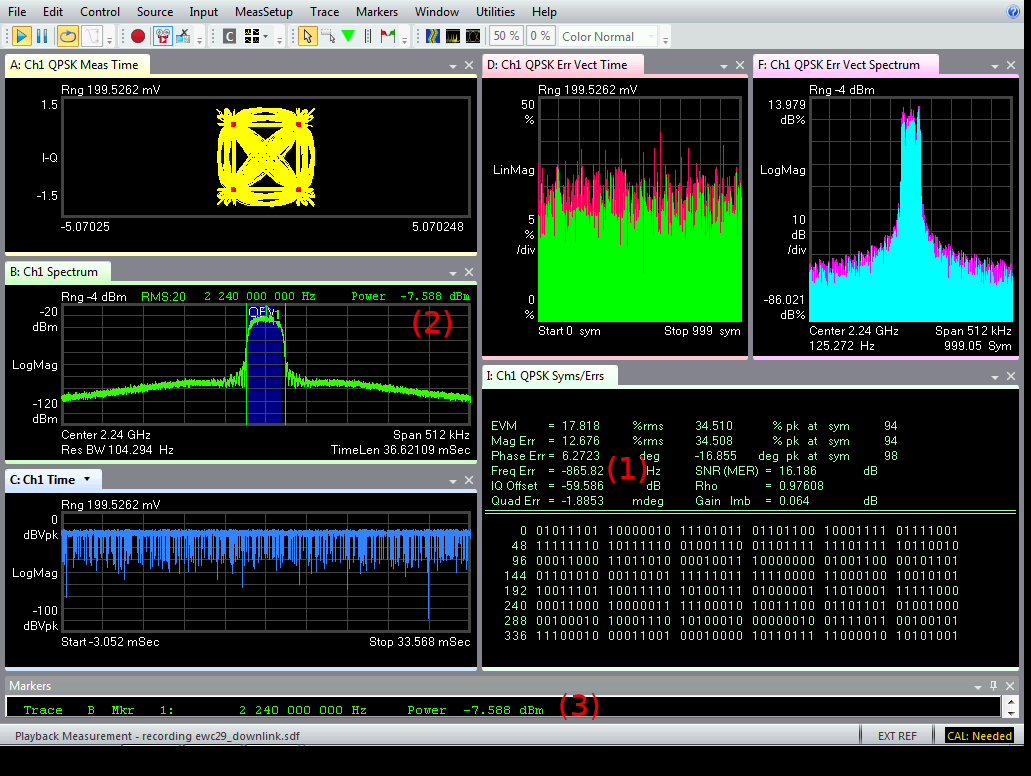
\includegraphics[width=0.53\textwidth]{figuras/downlink_EWC29.png}
        \end{center}
    }
}
% #endregion
% #region       MeasureRfTcCharacteristics
\newcommand{\MeasureRfTcCharacteristics}
{
    \stepcounter{Step}
    \immediate\write\myfile{\theSec,\theStep,MeasureRfTcCharacteristics}
    \procedurestep{\theSec}{\theStep}{EXE}{
    Measure RF signal characteristics .}{
    - Carrier frequency = $2062.6667\ MHz$ \\%$\leq\ 50KHz$\\
    - Output power ={ $-16.9\ dBm\pm1\ dB.$}\\%
    - Ocupied bandwidth $< 768\ 000\ Hz.$\\ % maximo permitido
    %- Modulation scheme = $QPSK(4\ states).$
    }{}{}
    \stepdetail{1}{0}{According to the image below, do the following:
        \begin{minipage}[t]{\linewidth}
            \begin{itemize}[nosep,after=\strut]
                \item In the Markers window, verify that the \textbf{carrier frequency} meets the expected values (1).
                \item In the Markers window, verify that the \textbf{output power} meets the expected values (2).
                \item In the Markers window, verify that the \textbf{Ocupied bandwidth} meets the expected values (3).
            \end{itemize}
        \end{minipage}
        \begin{center}
            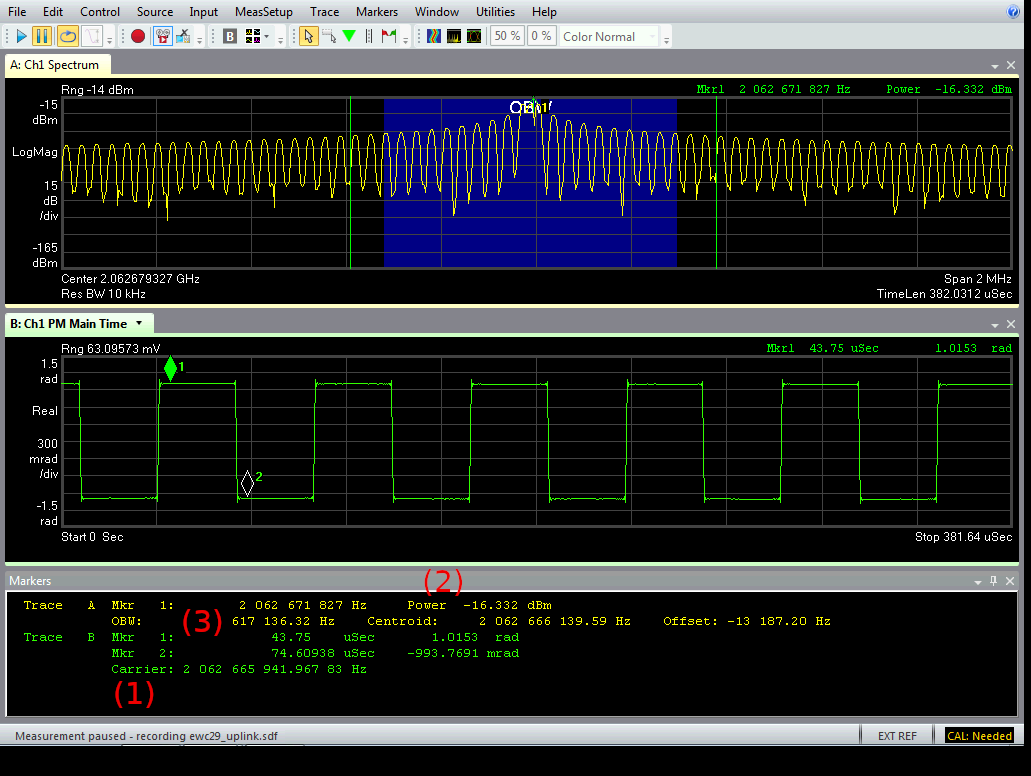
\includegraphics[width=0.53 \textwidth]{figuras/uplink_EWC29.png}
        \end{center}
    }
}
% #endregion

% #region       MeasureRfDataCharacteristics
\newcommand{\MeasureRfDataCharacteristics}
{
    \stepcounter{Step}
    \immediate\write\myfile{\theSec,\theStep,MeasureRfDataCharacteristics}
    \procedurestep{\theSec}{\theStep}{EXE}{
        Measure RF signal characteristics }{
        - Freq Err {$<\ 500KHz$} \\
        - Output power = $-10.6\ dBm\pm3\ dB.$\\% de portadora hay que tener unamedicion de lapotencia de la señal modulada al a entrada del GSE para hacer el calculo de elnace\\
        - Ocupied bandwidth  $\leq 162\ 000\ 000\ Hz.$\\ % decalculado usando (R/n)*(1+alfa)
        - Modulation scheme = $O-QPSK(4\ states).$}{}{}
    \stepdetail{1}{0}{According to the image below, do the following:
        \begin{minipage}[t]{\linewidth}
            \begin{itemize}[nosep,after=\strut]
                \item In window D (QPSK Syms/Errs), verify that \textbf{Freq Err} meets the expected values (1), the displayed Freq Err is the difference between the value configured in the VSA software and the measured value.
                \item In window B (Ch1: Spectrum), verify that the \textbf{output power} meets the expected values (2).
                \item In window A (QPSK Meas Time), verify that the \textbf{modulation scheme} is as expected.
                \item In the Markers window, verify that the \textbf{ocupied bandwidth} meets the expected values (3).
            \end{itemize}
        \end{minipage}
        \begin{center}
            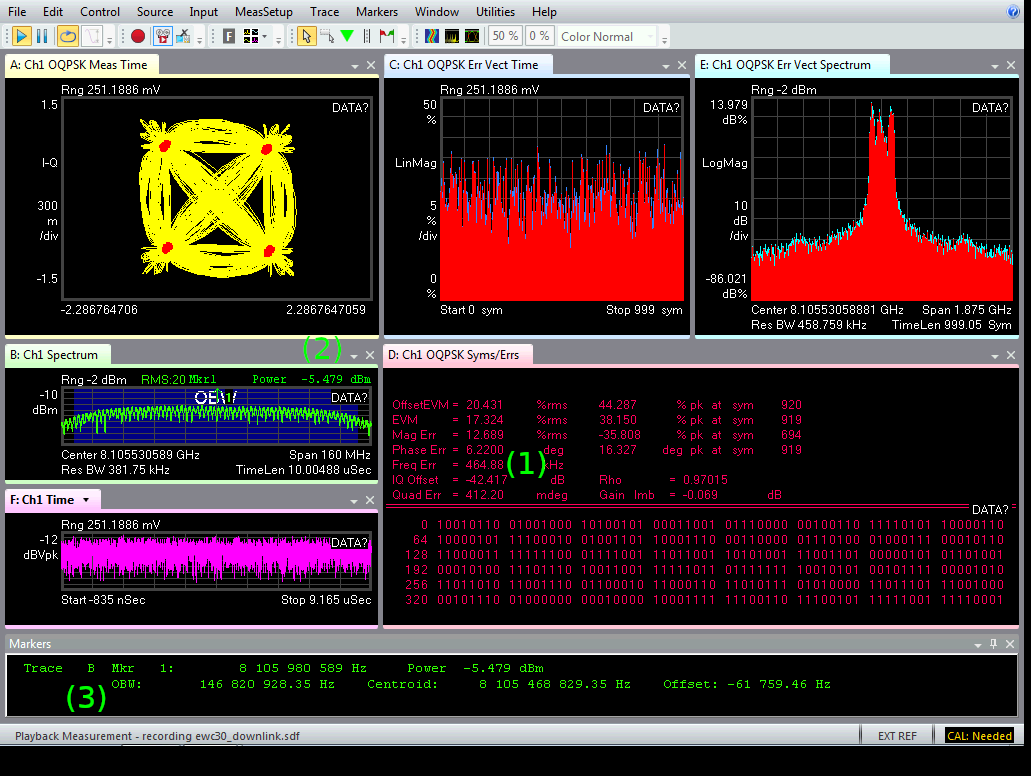
\includegraphics[width=0.41\textwidth]{figuras/downlink_EWC30.png}
        \end{center}
    }
}
% #endregion



% #region       MeasureRFOnCortexCrtQ
\newcommand{\ptmgse}{$P_{out} = -33.3\ dBm\pm3\ dB.$}
\newcommand{\MeasureRFOnCortexCrtQ}
{

    \stepcounter{Step}
    \procedurestep{\theSec}{\theStep}{EXE}{Measure IF carrier power in \textbf{\cortexQ.}}{-$P_{out} = -36.6\ dBm\pm3\ dB.$ \\
        -$PLL\ Locked$}{}{}
    \stepdetail{1}{0}{
        According to the figures below, do the following:
        \begin{itemize}[nosep,after=\strut]
            \item Go to MCS Cortex (\crtIP), in the \textbf{Global} window, click on the DCU (1).
            \item Go to Spectrum A tab of DCU.
            \begin{itemize}[nosep,after=\strut]
                \item Click in Enable button.
                \item Check that \textbf{PLL} field is locked (2).
                \item Check that the \textbf{IF Level} corresponds to the expected values (3).
            \end{itemize}
        \end{itemize}
        \vspace{-0.7cm}
        \begin{center}			
            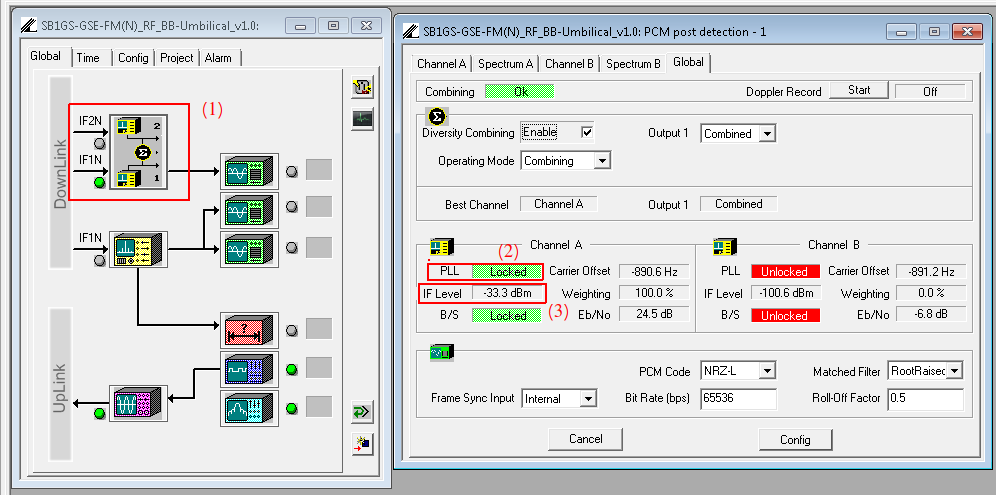
\includegraphics[width=0.7\textwidth]{figuras/N1-new}
        \end{center} 	 
        
    }
}
% #endregion
% #region       MuteSBandAttenuatorInterfaces
\newcommand{\MuteSBandAttenuatorInterfaces}
{
    \stepcounter{Step}
    \immediate\write\myfile{\theSec,\theStep,MuteSBandAttenuatorInterfaces}
    \procedurestep{\theSec}{\theStep}{EXE}{Disable \textbf{all} interfaces in the \textbf{\SBA}.}{All interfaces disabled.}{}{}
    \stepdetail{1}{0}{
        In the \sbmaSof software run on \vmWin (\vmWinIP):

        \begin{minipage}[t]{\linewidth}
            \begin{itemize}[nosep,after=\strut]
                \item  Go to the \textbf{Interface Selection} field of the \sbmaSof software and press \textbf{MUTE} button.
                \item Go to the \textbf{S-BAND ATTENUATOR} field and verify that  all indicators (N1, N2, Z1 and Z2) are red.
                      %\item Go to the \textbf{Interface Status} field and select \textbf{Monitor}.

            \end{itemize}
        \end{minipage}
    }
}
% #endregion
% #region       OpenCommandingWeb
\newcommand{\OpenCommandingWeb}
{
    \stepcounter{Step}
    \immediate\write\myfile{\theSec,\theStep,OpenCommandingWeb}
    \procedurestep{\theSec}{\theStep}{EXE}{Open the Commanding web.}{Commanding web open in a new tab.}{}{}
    \stepdetail{1}{0}{On the web browser go to \textbf{GS Web} and click the \textbf{Commanding} icon. The FC Commanding web will be open in a new tab.}
}
% #endregion
% #region       OpenLogMonitor
\newcommand{\OpenLogMonitor}
{
    \stepcounter{Step}
    \immediate\write\myfile{\theSec,\theStep,OpenLogMonitor}
    \procedurestep{\theSec}{\theStep}{EXE}{Open the Log Monitor web.}{Log Monitor web open in a new tab.}{}{}
    \stepdetail{1}{0}{On the web browser go to \textbf{GS Web} and click the \textbf{Log Monitor} icon. The Log Monitor web will be open in a new tab. Use the following credentials:
        \begin{itemize}[noitemsep]
            \item User: admin
            \item Password: admin
        \end{itemize}
    }
}
% #endregion
% #region       OpenStatusMonitor 
\newcommand{\OpenStatusMonitor}
{
    \stepcounter{Step}
    \immediate\write\myfile{\theSec,\theStep,OpenStatusMonitor}
    \procedurestep{\theSec}{\theStep}{EXE}{Open the Status Monitor web.}{Status Monitor web open in a new tab.}{}{}
    \stepdetail{1}{0}{On the web browser go to \textbf{GS Web} and click the \textbf{Status Monitor} icon. The Status Monitor web will be open in a new tab.}
}
% #endregion
% #region       OpenGsWebFromThinClient
\newcommand{\OpenGsWebFromThinClient}[1]
{
    \stepcounter{Step}
    \immediate\write\myfile{\theSec,\theStep,OpenGsWebFromThinClient}
    \procedurestep{\theSec}{\theStep}{EXE}{Open \textbf{SABIA-Mar Ground Segment} web from #1}{GS Web open in a new tab.}{}{}
    \stepdetail{1}{0}{From #1 open the FireFox browser. SABIA-Mar Ground Segment website will open automatically, if it was not the case access with the following parameters: \gsWebCredentials
    }
}
% #endregion
% #region       OpenNewSessionOnCommanding
\newcommand{\OpenNewSessionOnCommanding}
{
    \stepcounter{Step}
    \immediate\write\myfile{\theSec,\theStep,OpenNewSessionOnCommanding}
    \procedurestep{\theSec}{\theStep}{EXE}{Open a new session in Commanding }{The script runs successfully.}{}{}
    \stepdetail{1}{0}{On the web browser go to \textbf{Commanding} tab, select the command \textbf{System::open\_session} and click the \textbf{Run} button.}
}
% #endregion
% #region       OpenTeiWeb
\newcommand{\OpenTeiWeb}
{
    \stepcounter{Step}
    \immediate\write\myfile{\theSec,\theStep,OpenTeiWeb}
    \procedurestep{\theSec}{\theStep}{EXE}{Open the TM\&TC Extension web.}{TEIs web open in a new tab.}{}{}
    \stepdetail{1}{0}{On the web browser go to \textbf{GS Web} and click the \textbf{TM\&TC Extension} icon. The TEIs web will be open in a new tab.\\
    }
}
% #endregion
% #region       OpenSBMA
\newcommand{\OpenSBMA}
{
    \stepcounter{Step}
    \immediate\write\myfile{\theSec,\theStep,OpenSBMA}
    \procedurestep{\theSec}{\theStep}{EXE}{Open \textbf{\sbmaSof} software.}{\sbmaSof software open.}{}{}
    \stepdetail{1}{0}{On \vmWin (\vmWinIP) click the \textbf{\sbmaSof} icon located on the desktop.}
}
% #endregion
% #region       OpenSinterUnit
\newcommand{\OpenSinterUnit}
{
    \stepcounter{Step}
    \immediate\write\myfile{\theSec,\theStep,OpenSinterUnit}
    \procedurestep{\theSec}{\theStep}{EXE}{Open SInter unit.}{SInter unit open.}{}{}
    \stepdetail{1}{0}{On \vmFC (\vmFCIP) click the \textbf{SInter} icon located on the desktop.}
}
% #endregion
% #region       OpenXBMA
\newcommand{\OpenXBMA}
{
    \stepcounter{Step}
    \immediate\write\myfile{\theSec,\theStep,OpenXBMA}
    \procedurestep{\theSec}{\theStep}{EXE}{Open \textbf{\xbmaSof} software.}{\xbmaSof software open.}{}{}
    \stepdetail{1}{0}{On \vmWin (\vmWinIP) click the \textbf{\xbmaSof} icon located on the desktop.}
}
% #endregion

% #region       SessionIdRecord
\newcommand{\SessionIdRecord}{
    \sectionheader{}{Session ID Record}
    \immediate\write\myfile{\theSec,\theStep,SessionIdRecord}
    \procedurestep{}{}{WRI}{Record test session ID \sessionID.}{<YYYYMMDD-\#N>}{}{}
}
% #endregion

% #region       StartCegseSW
\newcommand{\StartCegseSW}[4]
{
    \stepcounter{Step}
    \immediate\write\myfile{\theSec,\theStep,StartCegseSW, CGF-FILE: #1 #2 #3}
    \procedurestep{\theSec}{\theStep}{EXE}
    {Start \comEgse{} SW using #1 #2 configuration file}
    {SW running in #1 #2 configuration}{}{}
    \stepdetail{1}{0}{
        #4
        \begin{itemize}[nosep,after=\strut]
            \item Locate “EGSE\_COM\_V1.0.4.exe” program icon on the desktop.
                  Double-click to open the icon and run the program.
            \item Write <YYYYMMDD-\#N> in “User” and “\subprocid" in “Test Code”. Click “Next”.
            \item In “Configuration File” search and load configuration file called
                  \textbf{#3} located in C:/USERS/EGSE COM/Documents/CFG/ folder.
            \item Click “Next” and press “OK” to confirm #1 configuration.
        \end{itemize}
    }
}
% #endregion
% #region       StartACQ{Main|Redundant}
\newcommand{\StartACQ}[1]
{
    \stepcounter{Step}
    \immediate\write\myfile{\theSec,\theStep,StartACQ, CHANNEL:#1}
    \procedurestep{\theSec}{\theStep}{EXE}{Start data acquisition on #1 Channel}{Acquisition started on #1 Channel}{}{}
    \stepdetail{1}{0}{
        In the \comEgse{} SW:
        \begin{itemize}[nosep,after=\strut]
            \item Go to the \textbf{COMM} tab and then go to the \textbf{Uplink} subtab.
            \item Switch channel selector to \textbf{RX #1}.
            \item Press \textbf{START RX TC} button.
            \item Verify that the pressed button changes to \textbf{STOP RX TC}
        \end{itemize}
    }
}
% #endregion
% #region       StartTeis
\newcommand{\StartTeis}
{
    \stepcounter{Step}
    \immediate\write\myfile{\theSec,\theStep,StartTeis}
    \procedurestep{\theSec}{\theStep}{EXE}{Start TEI of \gse}{Message "TEIs connected to TM\&TC Modem is showed.}{}{}
    \stepdetail{1}{0}{In the terminal window of \vmTesting (\vmTestingIP) run the following commands:
        \begin{itemize}[nosep,after=\strut]
            \item \texttt{cd \vmTestingTestFolderLocation\vmTestingTestFolderName/\sessionID }
            \item \texttt{python SB1GS-GSE-EM2.0-DemoTMTC.py RF 1800}
        \end{itemize}
        Wait until message "TEIs connected to TM\&TC Modem" is showed on terminal window.}
}
% #endregion

% #region       StartIngestionInCortexHdr
\newcommand{\StartIngestionInCortexHdr}
{
    \stepcounter{Step}
    \immediate\write\myfile{\theSec,\theStep,StartIngestionInCortexHdr}
    \procedurestep{\theSec}{\theStep}{EXE}{Start ingestion in \textbf{\cortexHDR} of \textbf{\gse} }{Ingestion started}{}{}
    \stepdetail{1}{0}{
        In Cortex MCS (\hdrIP) do the following:
        \begin{itemize}[nosep,after=\strut]
            \item In the \textbf{Global} window, click on the DRU-1.
            \item In the \textbf{Recording Global} window of DRU-1, click on \textbf{Start Recording} (Red button).
            \item Verify that the sign \textbf{Recording in Progress. Awaiting for Stop Command} appears in green.

        \end{itemize}
    }
}
% #endregion

% #region       StopIngestonInCortexHdr
\newcommand{\StopIngestonInCortexHdr}
{
    \stepcounter{Step}
    \immediate\write\myfile{\theSec,\theStep,StopIngestonInCortexHdr}
    \procedurestep{\theSec}{\theStep}{EXE}{Stop ingestion in \textbf{\cortexHDR} of \textbf{\gse} }{Ingestion stopped}{}{}
    \stepdetail{1}{0}{
        In Cortex MCS (\hdrIP)  go to \textbf{Recording Global} window of DRU-1 and in the \textbf{Recorder Programming} field click on \textbf{Stop Recording} button.
    }
}
% #endregion





% #region       StartVSASoftware
\newcommand{\StartVSASoftware}
{
    \stepcounter{Step}
    \immediate\write\myfile{\theSec,\theStep,StartVSASoftware}
    \procedurestep{\theSec}{\theStep}{EXE}{Initialize VSA software on the PXA.}{VSA software initialized.}{}{}
    \stepdetail{1}{0}{To initialize the VSA software do the following:
        \begin{minipage}[t]{\linewidth}
            \begin{itemize}[nosep,after=\strut]
                \item Press \textbf{Mode} button.
                \item Press \textbf{89601 VSA} key.
                \item Press \textbf{Start 89601B} key.
            \end{itemize}
        \end{minipage}
        \textbf{Note:} The VSA software takes approximately 5 minutes to initialize.}
}
% #endregion
% #region       StopCegseSW
\newcommand{\StopCegseSW}[1]
{
    \stepcounter{Step}
    \immediate\write\myfile{\theSec,\theStep,StopCegseSW}
    \procedurestep{\theSec}{\theStep}{EXE}{Stop the \comEgse{} SW by pressing the "Stop" button.}{The program ends and stops}{}{}
    \stepdetail{1}{0}{#1
     When you finish using the program in the \comEgse, you must press the \textbf{Stop} button to stop it.}
}

\newcommand{\VerifyStopCegseSW}
{
    \SimpleExeStep{Verify that the \comEgse{} SW is not running. }
    {\comEgse{} SW is not running.}
    {In \comEgse{} verify that the \comEgse{} SW is not running. }
}

% #endregion
% #region       StopACQ
\newcommand{\StopACQ}
{
    \stepcounter{Step}
    \immediate\write\myfile{\theSec,\theStep,StopACQ}
    \procedurestep{\theSec}{\theStep}{EXE}{Stop data acquisition}{Acquisition stopped}{}{}
    \stepdetail{1}{0}{
        In the \comEgse{} SW:
        \begin{itemize}[nosep,after=\strut]
            \item Go to the \textbf{COMM} tab and then to the \textbf{Uplink} subtab.
                  %\item Wait until bytes in \textbf{\#Bytes RX BS} is no longer incremented
            \item Press \textbf{STOP RX TC} button.
            \item Verify that the pressed button changes to \textbf{START RX TC}
        \end{itemize}}
}
% #endregion

% % #region       SendStoredFile
% \newcommand{\SendStoredFile}[1]
% {
%     \stepcounter{Step}
%     \immediate\write\myfile{\theSec,\theStep,SendStoredFile, FILE: \comEgseTestFolderLocation\comEgseTestFolderName{\bs}\sessionID\bs\procid\bs#1}
%     \procedurestep{\theSec}{\theStep}{EXE}{Start data transmission}{Data transmission started}{}{}
%     \stepdetail{1}{0}{
%         In the \comEgse{} SW:
%         \begin{itemize}
%             \item Go to the \textbf{COMM} tab and then go to the \textbf{Downlink} subtab.
%             \item On the \textbf{Stored Downlink File} box choose the file \texttt{#1} in
%                   \texttt{\comEgseTestFolderLocation\comEgseTestFolderName{\bs}\sessionID\bs\procid\bs} directory.
%             \item Switch file selector to \textbf{Send Stored Downlink File}
%             \item Press "Send" button.
%             \item Verify that “stage” box shows \textbf{“Sending S Band File”}.
%         \end{itemize}
%     }
% }
% % #endregion

\newcommand{\SendStoredFile}[1]
{
    \SimpleExeStep{
        Start data transmission
    }{
        Data transmission started
    }{
        In the \comEgse{}{} SW:
        \begin{minipage}[t]{\linewidth}
            \begin{itemize}[nosep,after=\strut]
                \item Go to the \textbf{COMM} tab and then go to the \textbf{Downlink} subtab.
                \item On the \textbf{Stored Downlink File} box choose the file \texttt{#1} in
                      \texttt{\comEgseTestFolderLocation{}\comEgseTestFolderName{}\bs{}\sessionID\bs\procid{}\bs} directory.
                \item Switch file selector to \textbf{Send Stored Downlink File}
                \item Turm off \textbf{NRZM-TM} indicator.
                \item Press \textbf{"Send"} button.
                \item Verify that “stage” box shows \textbf{“Sending S Band File”}.
            \end{itemize}
        \end{minipage}
    }
}



\newcommand{\SendGeneratedFileXBand}[2]
{
\SimpleExeStep{Start data transmission through the \textbf{#2 HV-HPC} interface}
{Data transmission started}
{   In the \comEgse{}{} SW:
    \begin{itemize}[nosep,after=\strut]
    \item Go to the \textbf{COMM} tab and then go to the \textbf{Downlink} subtab.
    \item Verify that \textbf{stage} box does not show \textbf{Sending X Band File} message.
    \item Switch file selector to \textbf{Send Generated Downlink File}
    \item Place the switch in \textbf{#1}
    \item Switch \textbf{Bit Endianness} selector to \textbf{Big}.
    \item Press \textbf{Send} button.
    \item Verify that \textbf{stage} box shows \textbf{Sending X Band File}.
\end{itemize}} 
}


% % #region       SendStoredFileXBand{File name}{HV-HPC Command}
% \newcommand{\SendStoredFileXBand}[2]
% {
%     \stepcounter{Step}
%     \immediate\write\myfile{\theSec,\theStep,SendStoredFileXBand, FILE:\comEgseTestFolderLocation\comEgseTestFolderName\string\ \sessionID\string\ \procid\string\ \subprocid\string\ #1 CMD:#2}
%     \procedurestep{\theSec}{\theStep}{EXE}{Start data transmission}{Data transmission started}{}{}
%     \stepdetail{1}{0}{
%         In the \comEgse{} SW:
%         \begin{itemize}[nosep,after=\strut]
%             \item Go to the \textbf{COMM} tab and then go to the \textbf{Downlink} subtab.
%             \item On the \textbf{Stored Downlink File} box choose the file \texttt{#1} in
%                   \texttt{\comEgseTestFolderLocation\comEgseTestFolderName{\bs}\sessionID\bs\procid\bs\subprocid\bs} directory.
%             \item Switch file selector to \textbf{Send Stored Downlink File}
%             \item Place the switch in "#2"
%             \item Press "Send" button.
%             \item Verify that “stage” box shows \textbf{“Sending X Band File”}.
%         \end{itemize}
%     }
% }
% % #endregion



% #region       SendGeneratedFile
\newcommand{\SendGeneratedFile}[2]
{
    \stepcounter{Step}
    \immediate\write\myfile{\theSec,\theStep,SendGeneratedFile}
    \procedurestep{\theSec}{\theStep}{EXE}
    {Start TM transmission}{ TM transmission started}{}{}
    \stepdetail{1}{0}{In the CEGSE SW: 
        \begin{itemize}[nosep,after=\strut]
            \item Go to COMM tab, then select DOWNLINK subtab.
            \item Place the switch in \textbf{Send Generated Downlink File}.
            \item Turn off \textbf{NRZM-TM} indicator.
            \item Press Send button.
            \item Verify that \textbf{stage} box shows \textbf{Sending S Band File}.
        \end{itemize}
        \textbf{Note:} Generated Downlink file has #1 frames (#2 minutes)
    }
}
% #endregion

% #region       SendGeneratedFileXBand
% \newcommand{\SendGeneratedFileXBand}[1]
% {
%     \stepcounter{Step}
%     \immediate\write\myfile{\theSec,\theStep,SendGeneratedFileXBand}
%     \procedurestep{\theSec}{\theStep}{EXE}
%     {Start sending down-link file}{Stage box shows "Sending...."}{}{}
%     \stepdetail{1}{0}{
%         \begin{itemize}[nosep,after=\strut]
%             \item On \comEgse{} GUI select COMM tab, then select DOWNLINK subtab.
%             \item Place the switch in "Send Generated Downlink File"
%             \item Place the switch in "#1"
%             \item Press Send button.
%             \item Verify that “stage” box shows “Sending X Band File”.
%         \end{itemize}
%     }
% }
% #endregion


% #region       SyncAndVerifyNumberOfTC
\newcommand{\SyncAndVerifyNumberOfTC}[1]
{
    \stepcounter{Step}
    \immediate\write\myfile{\theSec,\theStep,SyncAndVerifyNumberOfTC EXPECTED:#1}
    \procedurestep{\theSec}{\theStep}{EXE}{Synchronize acquired data on \comEgse.}{#1 frames Synchronized}{}{}
    \stepdetail{1}{0}{
        On \comEgse{} GUI go to COM/UPLINK subtab and do the following:
        \begin{itemize}[nosep,after=\strut]
            \item Turn on \textbf{Delete Header and CRC} indicator.
            \item Turn off \textbf{InvertData} and \textbf{NRZM-TC} indicators.
            \item Press \textbf{Sync File} button in SW of the \comEgse{}
            \item Wait until \textbf{Sync Finished} indicator turns on
            \item Verify that number of Synchronized frames is equals to the expected value.
        \end{itemize}.}
}
% #endregion
% #region       TSMAliveness
\newcommand{\TSMAliveness}[4]
{
    \stepcounter{Step}
    \immediate\write\myfile{\theSec,\theStep,TSMAliveness,PIN(+)=#3 PIN(-)=#4 BOB=#2 SIGNAL=#1 }
    \procedurestep{\theSec}{\theStep}{EXE}{TSM #1 interfaces aliveness.}{$Voltage\approx 12 V$}{}{}
    \stepdetail{1}{0}{
        Set the multimeter to measure voltage and hold the Max value.\\
        Connect the multimeter probes to pins \textbf{#3(+)} and \textbf{#4(-)} of the \textbf{#2 BOB}.\\
        \textbf{Note:} Multimeter must be set to register the Max value due to \comEgse{} reading architecture.
    }
}
% #endregion


\newcommand{\TSMAlivenessXband}[4]
{
	\SimpleExeStep{
		TSM #1 interfaces aliveness.
	}{
		$Voltage\approx 6 V$
	}{
		Set the multimeter to measure voltage and hold the Max value.\
		Connect the $47 K\Omega$ resistor between pin \textbf{#3(+)} and \textbf{#4(-)} of the \textbf{#2 BOB}.\
		Measure voltage across the resistor.\
		\textbf{Note:} Multimeter must be set to register the Max value due to \comEgse{}{} reading architecture.
	}
}










% #region       TSMAlivenessXBand
\newcommand{\TSMAlivenessXbandOld}[4]
{
    \stepcounter{Step}
    \immediate\write\myfile{\theSec,\theStep,TSMAlivenessXband,PIN(+)=#3 PIN(-)=#4 BOB=#2 SIGNAL=#1}
    \procedurestep{\theSec}{\theStep}{EXE}{TSM #1 interfaces aliveness.}{$Voltage\approx 12 V$}{}{}
    \stepdetail{1}{0}{
        Set the multimeter to measure voltage.\\
        Connect the multimeter probes to pins #3(+) and #4(-) of the #2 BOB.
    }
}
% #endregion

% #region       TurnOnOffVbusSBand
\newcommand{\TurnOnOffVbusSBand}[2]
{
    \stepcounter{Step}
    \immediate\write\myfile{\theSec,\theStep,TurnOnOffVbusSBand PART: #1 ACTION: #2 }
    \procedurestep{\theSec}{\theStep}{EXE}{Turn #2 VBUS of #1 part}{{#1}29S led is #2.}{}{}
    \stepdetail{1}{0}{In the \comEgse{} SW press \textbf{EWC29#1} button. In the AD-HOC box verify \textbf{{#1}29S} led status.}
}
% #endregion
\newcommand{\VerifyOffVbusSBand}[1]
{
    \SimpleExeStep{Verify #1 Part VBUS shutdown.}
    {{#1}29S led is off}
    {In the AD-HOC box verify \textbf{{#1}29S} led status is off.}
}
%new
\newcommand{\VerifyOffVbusXBand}[1]
{
    \SimpleExeStep{Verify #1 Part VBUS shutdown.}
    {{#1}30S led is off}
    {In the AD-HOC box verify \textbf{{#1}30S} led status is off.}
}

% #region       TurnOnOffVbusXBand
\newcommand{\TurnOnOffVbusXBand}[2]
{
    % \stepcounter{Step}
    % \immediate\write\myfile{\theSec,\theStep,TurnOnOffVbusXBand, ACTION=#1}
    % \procedurestep{\theSec}{\theStep}{EXE}{Turn #1 VBUS of TX}{TX30X led is #1.}{}{}
    % \stepdetail{1}{0}{#2 \\
    
    % In the \comEgse{} SW press \textbf{EWC30} button. In the AD-HOC
    %     box verify \textbf{TX30X} led status.}

    \SimpleExeStep{Turn #1 VBUS of TX}{TX30X led is #1.}{#2
     In the \comEgse{} SW press \textbf{EWC30} button. In the AD-HOC
    box verify \textbf{TX30X} led status.}

}
% #endregion


% #region       TurnOnOffPSU
\newcommand{\TurnOnOffPSU}[1]
{
    \stepcounter{Step}
    \immediate\write\myfile{\theSec,\theStep,TurnOnOffPSU, ACTION=#1}
    \procedurestep{\theSec}{\theStep}{EXE}{Turn #1 the PSU switch of the Ad-Hoc box.}{PSU LED indicator should turn #1}{}{}
    \stepdetail{1}{0}{Turn #1 the PSU by pressing the switch in the center of the Ad-Hoc box. \\ Verify that the LED on the PSU has turned #1
        when the switch is turned #1.}
}
% #endregion
% #region       TurnOffMainSwitch
\newcommand{\TurnOffMainSwitch}
{
    \stepcounter{Step}
    \immediate\write\myfile{\theSec,\theStep,TurnOffMainSwitch}
    \procedurestep{\theSec}{\theStep}{EXE}{Turn off the main switch of the Ad-Hoc box.}{The main switch light must be turned off}{}{}
    \stepdetail{1}{0}{Turn off the main switch of the Ad-Hoc box.}
}
% #endregion
% #region       TurnOnMainSwitch
\newcommand{\TurnOnMainSwitch}
{
    \stepcounter{Step}
    \immediate\write\myfile{\theSec,\theStep,TurnOnMainSwitch}
    \procedurestep{\theSec}{\theStep}{EXE}{Turn on the main switch of the Ad-Hoc box.}{The main switch light must be turned on}{}{}
    \stepdetail{1}{0}{Turn on the main switch of the Ad-Hoc box.}
}
% #endregion
% #region       TestSBDLLoops
\newcommand{\TestSBDLLoops}[2]
{
    \stepcounter{Step}
    \immediate\write\myfile{\theSec,\theStep,TestSBDLLoops OUTPUT:#1 INPUT:#2}
    \procedurestep{\theSec}{\theStep}{EXE}{Verify loop between #1 and #2}{#2 status changed}{}{}
    \stepdetail{1}{0}{In \comEgse{} SW go to SBDL\&BDM tab and do the following actions:
        \begin{itemize}[nosep,after=\strut]
            \item Press \textbf{#1} button (activate).
            \item Verify that \textbf{#2} indicator turn on.
            \item Press \textbf{#1} button (deactivate).
            \item Verify that \textbf{#2} indicator turn off.
        \end{itemize}
    }
}
% #endregion
% #region       RDPToCortexFromThinClient[\thinTT C]
\newcommand{\RDPToCortexFromThinClient}[1]
{
    \stepcounter{Step}
    \immediate\write\myfile{\theSec,\theStep,RDPToCortexFromThinClient,IP=\crtIP. USR=cortex PSW=cortex}
    \procedurestep{\theSec}{\theStep}{EXE}{\textbf{RDP connection} to  \cortexQ from #1.}{ #1 connected a \cortexQ}{}{}
    \stepdetail{1}{0}{From the #1 open the Remote Desktop Connection and connect to IP: \crtIP
        \begin{itemize}[nosep,after=\strut]
            \item \texttt{User: cortex}
            \item \texttt{Password: cortex}
        \end{itemize}
    }
}
% #endregion
% #region       RDPToPXIFromThinClient
\newcommand{\RDPToPXIFromThinClient}[1]
{
    \stepcounter{Step}
    \immediate\write\myfile{\theSec,\theStep,RDPToPXIFromThinClient,IP=\comEgseIP. USR=EGSE COM PSW=Conae1234}
    \procedurestep{\theSec}{\theStep}{EXE}{\textbf{RDP connection} to  \comEgse{} from Thin client \textbf{#1}.}{ Thin Client  \textbf{OW DATA A} connected to \comEgse}{}{}
    \stepdetail{1}{0}{From the #1 open the Remote Desktop Connection and connect to IP: \comEgseIP
        \begin{itemize}[nosep,after=\strut]
            \item \texttt{User: EGSE COM }
            \item \texttt{Password: Conae1234 }
        \end{itemize}
    }
}
% #endregion
% #region       RDPToMgmtFromThinClient
\newcommand{\RDPToMgmtFromThinClient}[1]
{
    \stepcounter{Step}
    \immediate\write\myfile{\theSec,\theStep,RDPToMgmtFromThinClient,IP=\vmTestingIP. USR=administrator PSW=Sb1.C0n43}
    \procedurestep{\theSec}{\theStep}{EXE}{\textbf{RDP connection} to  \vmTesting from #1.}{ \thinDT A connected to \vmTesting}{}{}
    \stepdetail{1}{0}{From the #1 open the Remote Desktop Connection and connect to IP: \vmTestingIP
        \begin{itemize}[nosep,after=\strut]
            \item {User: administrator}
            \item {Password: Sb1.C0n43}
        \end{itemize}
    }
}
% #endregion
% #region       RDPToSbaVmFromThinClientC
\newcommand{\RDPToSbaVmFromThinClientA}
{
    \stepcounter{Step}
    \immediate\write\myfile{\theSec,\theStep,RDPToSbaVmFromThinClientA,IP=\vmWinIP. USR=admin PSW=Sb1.C0n43}
    \procedurestep{\theSec}{\theStep}{EXE}{\textbf{RDP connection} to \vmWin from \thinTT A.}{ \thinTT A connected a \vmWin}{}{}
    \stepdetail{1}{0}{From the \thinTT A open the Remote Desktop Connection and connect to IP: \vmWinIP
        \begin{itemize}[nosep,after=\strut]
            \item \texttt{User: admin}
            \item \texttt{Password: Sb1.C0n43}
        \end{itemize}
    }
}
% #endregion
% #region       RDPToSinterVmFromThinClientC
\newcommand{\RDPToSinterVmFromThinClientA}
{
    \stepcounter{Step}
    \immediate\write\myfile{\theSec,\theStep,RDPToSinterVmFromThinClientA,IP=\vmFCIP. USR=administrator PSW=Sb1.C0n43}
    \procedurestep{\theSec}{\theStep}{EXE}{\textbf{RDP connection} to  \vmFC from \thinTT A.}{ \thinTT A connected a \vmFC}{}{}
    \stepdetail{1}{0}{From the \thinTT A open the Remote Desktop Connection and connect to IP: \vmFCIP
        \begin{itemize}[nosep,after=\strut]
            \item \texttt{User: administrator}
            \item \texttt{Password: Sb1.C0n43}
        \end{itemize}
    }
}
% #endregion
% #region       RemoveTransportLayer
\newcommand{\RemoveTransportLayer}[2]
{
    \stepcounter{Step}
    \immediate\write\myfile{\theSec,\theStep,RemoveTransportLayer}
    \procedurestep{\theSec}{\theStep}{EXE}
    {Remove Transport Layer}{VC ID = 1\\\#Frames = #2\\Generated File = On}{}{}
    \stepdetail{1}{0}{
        \begin{itemize}[nosep,after=\strut]
            \item Execute TM\_Downlink\_File\_to\_Payload\_File\_Converter from Desktop icon.
            \item Press the folder icon next to “File path to read” and select the downloaded file on
                  \comEgseTestFolderLocation\comEgseTestFolderName\bs\sessionID\bs\procid\bs\subprocid{} folder.
            \item 	In “Telemetry Selector”, select #1
            \item 	Press the folder icon next to “Destination directory path” and select the
                  \comEgseTestFolderLocation\comEgseTestFolderName\bs\sessionID\bs\procid\bs\subprocid{} folder.
            \item Press the “Remove Transport Layer” button to create the final file to be compared
        \end{itemize}
    }
}
% #endregion
% #region       RegisterTempAndHumidity
\newcommand{\RegisterTempAndHumidity}
{
    \stepcounter{Step}
    \immediate\write\myfile{\theSec,\theStep,RegisterTempAndHumidity}
    \procedurestep{\theSec}{\theStep}{EXE}{Verify environmental \textbf{temperature} levels.}{+23 °C ± 3 °C}{}{}
    \stepdetail{1}{0}{Verify that the environmental temperature level in the test site 
    is according to the required levels.}
    %
    \stepcounter{Step}
    %\immediate\write\myfile{\theSec,\theStep,TBC}
    \procedurestep{\theSec}{\theStep}{EXE}{Take note of the environmental humidity.}{Humidity}{}{}
    \stepdetail{1}{0}{Take note the environmental humidity in the test site.}
    %
}
% #endregion

% #region       RegisterTemp
\newcommand{\RegisterTemp}
{
    \stepcounter{Step}
    \immediate\write\myfile{|\theSec|\theStep|RegisterTempAndHumidity|}
    \procedurestep{\theSec}{\theStep}{EXE}{Verify environmental \textbf{temperature} levels.}{+23 °C ± 3 °C}{\Result}{\Status}
    \stepdetail{1}{0}{Verify in the sensor located on working table that the environmental temperature level is according to the required levels.}
}

% #endregion
% #region       RegisterHumidity
\newcommand{\RegisterHumidity}
{
    \stepcounter{Step}
    %\immediate\write\myfile{|\theSec|\theStep|TBC|}
    \procedurestep{\theSec}{\theStep}{EXE}{Take note of the environmental humidity.}{Humidity}{\Result}{\Status}
    \stepdetail{1}{0}{Take note the environmental humidity from the sensor located on working table.\\ \Extradetail}
    %
}
% #endregion


% #region       UnzipDataSetOnPxi
\newcommand{\UnzipDataSetOnPxi}
{
    \stepcounter{Step}
    \immediate\write\myfile{\theSec,\theStep,UnzipDataSetOnPxi Folder: C:/Users/EGSE COM/Documents/COMM-SS-EM-FT/\sessionID }
    \procedurestep{\theSec}{\theStep}{EXE}{Unzip the dataset.}{Dataset unzipped.}{}{}
    \stepdetail{1}{0}{
        \begin{itemize}[nosep,after=\strut]
            \item Open File Explorer and go to \textbf{C:/Users/EGSE COM/Documents/COMM-SS-FM/\sessionID}
                \item Right-click on \textbf{\datasetNameone{}}
                \textbf{\datasetNametwo{}.zip} and select \textbf{"7-Zip"} option.
                \item In the displayed menu select \textbf{Extract here} option.
                \item Verify that decompression process ends without error.
        \end{itemize}
        \textbf{Note}: If a file with the same name already exists, replace it.
    }
}
% #endregion
% #region       UnzipDataSetOnMgmt
\newcommand{\UnzipDataSetOnMgmt}
{
    \stepcounter{Step}
    \immediate\write\myfile{\theSec,\theStep,UnzipDataSetOnMgmt}
    \procedurestep{\theSec}{\theStep}{EXE}{Unzip the document dataset.}{Dataset unzipped.}{}{}
    \stepdetail{1}{0}{
        In a terminal window of \vmTesting (\vmTestingIP)  run the following commands:
        \begin{itemize}[nosep,after=\strut]
            \item \texttt{cd /verification}
            \item \texttt{mv \datasetName.zip \ /verification/\sessionID/ }
            \item \texttt{cd /verification/\sessionID/}
            \item \texttt{unzip \datasetName.zip }
            \item \texttt{rm \datasetName.zip}
        \end{itemize} }
}
% #endregion
% #region       VerifySBandDownConverter
\newcommand{\VerifySBandDownConverter}
{
    \stepcounter{Step}
    \immediate\write\myfile{\theSec,\theStep,VerifySBandDownConverter}
    \procedurestep{\theSec}{\theStep}{EXE}{Verify \textbf{\sdnc} configuration}{
        - Frequency 2240.000000 MHz.\\ - RF output ON.\\- Locked to external reference.\\- Attenuation 15 dB.}{}{}
    \stepdetail{1}{0}{
        See the display on the front panel of \supc, should be displayed :\\
        \begin{minipage}[t]{\linewidth}
            \begin{itemize}[nosep,after=\strut]
                \item \textbf{RF=2240.000000MHz}
                \item \textbf{RF ON}
                \item \textbf{EXT}
                \item \textbf{ATTEN=15.00dB}
            \end{itemize} \end{minipage} \\~\\
        Note: If the front panel display is not on, press the \textbf{Enter} button.
    }
}
% #endregion
% #region       TakeScreenShotInCortex
\newcommand{\TakeScreenShotInCortex}
{
    \stepcounter{Step}
    \immediate\write\myfile{\theSec,\theStep,TakeScreenShotInCortex}
    \procedurestep{\theSec}{\theStep}{EXE}{Take screenshot of signal measurement.}{\texttt{<filename.png>} saved.}{}{}
    \stepdetail{1}{0}{Take the screenshot of the \cortexQ, save it in the \modemCap{{}}cortex-screenshot-013-02 directory
        and take note the saved file name. This could be done by pressing the \textbf{print screen key} and using the Paint software. }
}
% #endregion


% #region       TakePhotosOfDutConnections
\newcommand{\TakePhotosOfDutConnections}
{
    \stepcounter{Step}
    \immediate\write\myfile{\theSec,\theStep,TakePhotosOfDutConnections}
    \procedurestep{\theSec}{\theStep}{EXE}{Take photos of the setup and DUT connections.}{Photos taken.}{}{}
    \stepdetail{1}{0}{Take photos of setup and DUT connections.}
}
% #endregion

% #region       SaveEvidencePhotos
\newcommand{\SaveEvidencePhotos}
{
    % \stepcounter{Step}
    % \immediate\write\myfile{\theSec,\theStep,SaveEvidencePhotos}
    % \procedurestep{\theSec}{\theStep}{EXE}{Save evidence photos}{Evidence photos saved}{}{}
    % \stepdetail{1}{0}{
    %     Create \textbf{pictures} folder on 
    %     \comEgseTestFolderLocation\comEgseTestFolderName
    %     \bs\sessionID\bs\procid\bs\subprocid{} 
    %      save all photos taken during the DUT connections.
    % }
\SimpleExeStep{Save evidence photos}{Evidence photos saved}{ Create \textbf{pictures} folder on 
\comEgseTestFolderLocation\comEgseTestFolderName
\bs\sessionID\bs\procid\bs\subprocid{} 
 save all photos taken during the DUT connections.}

    }



% #endregion


% #region       VerifyCarrierOffInCortex
\newcommand{\VerifyCarrierOffInCortex}
{
    \stepcounter{Step}
    \immediate\write\myfile{\theSec,\theStep,VerifyCarrierOffInCortex}
    \procedurestep{\theSec}{\theStep}{EXE}{Verify absence of TM carrier in \textbf{\cortexQ of \gse.}}{Absent TM carrier}{}{}
    \stepdetail{1}{0}{

        According to the figures below, do the following:
        \begin{itemize}[nosep,after=\strut]
            \item Go to MCS Cortex (\crtIP), in the \textbf{Global} window, click on the TMU-B (1).
            \item In the \textbf{Status} window of TMU-B.
                  \begin{itemize}[nosep,after=\strut]
                      \item Check that \textbf{IFR} field is Unlocked (2).
                      \item Check absence of \textbf{IF level} in the central field (3).
                  \end{itemize}
        \end{itemize}
        \vspace{-0.7cm}
        \begin{center}
            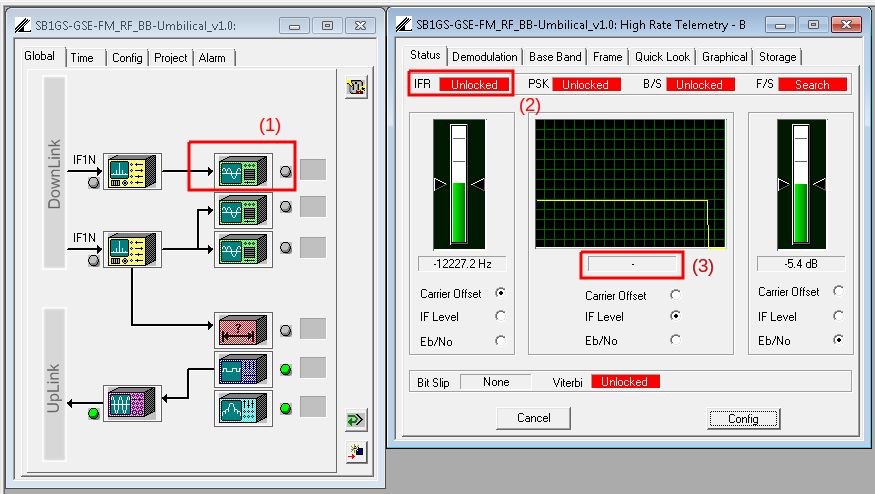
\includegraphics[width=0.6\textwidth]{figuras/sinpower_cortex_rx_gse-013-02}
        \end{center}
    }
}
% #endregion

% #region       TakeScreenShotOfVCWindowInCortex
\newcommand{\TakeScreenShotOfVCWindowInCortex}
{
    \stepcounter{Step}
    \immediate\write\myfile{\theSec,\theStep,TakeScreenShotOfVCWindowInCortex}
    \procedurestep{\theSec}{\theStep}{EXE}{Take screenshot of {Virtual Channels} window}{<filename.png>}{}{}
    \stepdetail{1}{0}{
        In Cortex MCS (\hdrIP) go to \textbf{Virtual Channels} window of DRU-A and click on the \textbf{VC Sort Value}
        column to sort it from highest to lowest. Take the screenshot of the \cortexHDR, save it in the \hdrCap {{}}cortex-\screen-01 directory and take note the saved file name. This could be done by pressing the \textbf{print screen key} and using the Paint software.
    }
}
% #endregion


% #region       VerifyLockedInCortexHdr
\newcommand{\VerifyLockedInCortexHdr}[1]
{
    \stepcounter{Step}
    \immediate\write\myfile{|\theSec|\theStep|VerifyLockedInCortexHdr|}
    \procedurestep{\theSec}{\theStep}{EXE}{Verify locked status  in DPU-#1 of \textbf{\cortexHDR{}} of \textbf{\gse} }{
PLL is locked and stable.\\
B/S is locked and stable.\\
Viterbi is locked and stable.\\
F/S is locked and stable.

}{}{}
    \stepdetail{1}{0}{
        Go to  Cortex MCS (\hdrIP{}) of \fmr{} and in the open DPU-#1 window do the following:
        \begin{minipage}[t]{\linewidth}
            \begin{itemize}[nosep,after=\strut]
                    \item Verify that PLL is locked.
                    \item Verify that B/S is locked.
                    \item Verify that Viterbi is Locked.
                    \item Verify that F/S is locked.
            \end{itemize}
        \end{minipage}
        Verify for 30 seconds that none of them unlock.
    }
}




% \newcommand{\VerifyLockedInCortexHdr}[1]
% {
%     \stepcounter{Step}
%     \immediate\write\myfile{\theSec,\theStep,VerifyLockedInCortexHdr}
%     \procedurestep{\theSec}{\theStep}{EXE}{Verify locked  in \textbf{\cortexHDR} of \textbf{\gse} }{\cortexHDR locked}{}{}
%     \stepdetail{1}{0}{
%         In Cortex MCS (\hdrIP) go to \textbf{Recording Global} window of DRU-#1 and verify that F/S is locked.
%     }
% }
% #endregion

% #region       VerifySbandUpConverter 
% SBandUpConverter
\newcommand{\VerifySbandUpConverter}
{
    \stepcounter{Step}
    \immediate\write\myfile{\theSec,\theStep,VerifySbandUpConverter}
    \procedurestep{\theSec}{\theStep}{EXE}{Verify \textbf{\supc} configuration}{
        - Frequency 2062.666700 MHz.\\ - RF output OFF.\\ - Locked to external reference.\\- Attenuation 10 dB.

    }{}{}
    \stepdetail{1}{0}{
        See the display on the front panel of \supc, should be displayed :\\
        \begin{minipage}[t]{\linewidth}
            \begin{itemize}[nosep,after=\strut]
                \item \textbf{RF=2062.666700MHz}
                \item \textbf{RF OFF}
                \item \textbf{EXT}
                \item \textbf{ATTEN=10.00dB}
            \end{itemize} \end{minipage} \\~\\
        Note: If the front panel display is not on, press the \textbf{Enter} button.
    }
}
% #endregion
% #region       VerifyXBandDownConverterOne
\newcommand{\VerifyXBandDownConverterOne}
{
    \stepcounter{Step}
    \immediate\write\myfile{\theSec,\theStep,VerifyXBandDownConverterOne}
    \procedurestep{\theSec}{\theStep}{EXE}{Verify \textbf{\xdnc N1} configuration. }{

        %\begin{minipage}[t]{\linewidth}
        \begin{itemize}[nosep,after=\strut]
            \item RF = 8106.0 MHz
            \item Aten = 6 dB % 6 N1 y 4 N2 de FMR
            \item RF = ON
        \end{itemize}
        %\end{minipage} \\~\\.
    }{}{}
    \stepdetail{1}{0}{

        In the terminal window of \vmTesting (\vmTestingIP) run the following commands:
        \begin{itemize}[noitemsep]
            \item \texttt{cd \xdncDir }
            \item \texttt{python \xdnONEpy}
        \end{itemize}
        In the displayed menu, verify that the parameters are configured according to the expected values. Then enter the number 5 and press enter to exit the menu.
    }
}
% #endregion

% #region       VerifyXBandDownConverterTwo
\newcommand{\VerifyXBandDownConverterTwo}
{
    \stepcounter{Step}
    \immediate\write\myfile{\theSec,\theStep,VerifyXBandDownConverterTwo}
    \procedurestep{\theSec}{\theStep}{EXE}{Verify \textbf{\xdnc N2} configuration. }{

        %\begin{minipage}[t]{\linewidth}
        \begin{itemize}[nosep,after=\strut]
            \item RF = 8269.0 MHz
            \item Aten = 4 dB % 6 N1 y 4 N2 de FMR
            \item RF = ON
        \end{itemize}
        %\end{minipage} \\~\\.
    }{}{}
    \stepdetail{1}{0}{

        In the terminal window of \vmTesting (\vmTestingIP) run the following commands:
        \begin{itemize}[noitemsep]
            \item \texttt{cd \xdncDir }
            \item \texttt{python \xdnTWOpy}
        \end{itemize}
        In the displayed menu, verify that the parameters are configured according to the expected values. Then enter the number 5 and press enter to exit the menu.
    }
}
% #endregion
% #region       ConfigureXBandDownConverterOne
\newcommand{\ConfigureXBandDownConverterOne}[1]
{
    \stepcounter{Step}
    \immediate\write\myfile{|\theSec|\theStep|ConfigureXBandDownConverterOne|}
    \procedurestep{\theSec}{\theStep}{EXE}{Configure \textbf{\xdnc{} N1}.}{
        \begin{minipage}[t]{\linewidth}
            \begin{itemize}[nosep,after=\strut,leftmargin=*]
                \item RF = 8106.0 MHz
                \item Aten = #1
                \item RF = ON
            \end{itemize}
        \end{minipage}
    }{\Result}{\Status}
    \stepdetail{1}{0}{
    	Note: Skip this step if \textbf{EWC30-FM2} is under test.\\ \vspace{5mm}
        In the terminal window of \vmTesting{} (\vmTestingIP{}) of \fmn{} run the following commands:
        \begin{minipage}[t]{\linewidth}
            \begin{itemize}[nosep,after=\strut]
                \item \texttt{cd \xdncDir{} }
                \item \texttt{python \xdnONEpy{}}
            \end{itemize}
        \end{minipage}
        In the displayed menu, do the following:
        \begin{minipage}[t]{\linewidth}
            \begin{itemize}[nosep,after=\strut]
                \item Configure Aten = #1.
                \item Verify that Freq = 8106 MHz.
                \item Verify that RF = ON
            \end{itemize}
        \end{minipage}
        Then enter the number 5 and press enter to exit the menu.\\
        \Extradetail
    }
}
% #endregion

%VerifyXBandDownConverterTwo
% #region       ConfigureXBandDownConverterTwo
\newcommand{\ConfigureXBandDownConverterTwo}[1]
{
    \stepcounter{Step}
    \immediate\write\myfile{|\theSec|\theStep|ConfigureXBandDownConverterTwo|}
    \procedurestep{\theSec}{\theStep}{EXE}{Configure \textbf{\xdnc{} N2}.}{
        \begin{minipage}[t]{\linewidth}
            \begin{itemize}[nosep,after=\strut,leftmargin=*]
                \item RF = 8269.0 MHz
                \item Aten = #1
                \item RF = ON
            \end{itemize}
        \end{minipage}
    }{\Result}{\Status}
    \stepdetail{1}{0}{
    	Note: Skip this step if \textbf{EWC30-FM1} is under test.\\ \vspace{5mm}

        In the terminal window of \vmTesting{} (\vmTestingIP{}) of \fmn{} run the following commands:
        \begin{minipage}[t]{\linewidth}
            \begin{itemize}[nosep,after=\strut]
                \item \texttt{cd \xdncDir{} }
                \item \texttt{python \xdnTWOpy{}}
            \end{itemize}
        \end{minipage}
        In the displayed menu, do the following:
        \begin{minipage}[t]{\linewidth}
            \begin{itemize}[nosep,after=\strut]
                \item Configure Aten = #1.
                \item Verify that Freq = 8269 MHz.
                \item Verify that RF = ON
            \end{itemize}
        \end{minipage}
        Then enter the number 5 and press enter to exit the menu.\\
        \Extradetail
    }
}
% #endregion
%%%%%%%%%%%%%%%%%%%%%%%%%%%%%%%%%%%%%%%%%%%%%%%%%%%%%%%%%%%%%%%%%%%%%%%
%%%%%%%%%%%%%%%%%%%%%%%%%%%%%%%%%%%%%%%%%%%%%%%%%%%%%%%%%%%%%%%%%%%%%%%

% #region       SetXbmaAttenuationTo
\newcommand{\SetXbmaAttenuationToq}[2]
{
    \stepcounter{Step}
    \procedurestep{\theSec}{\theStep}{EXE}{Set attenuation of \textbf{\XBMA{}}.}{Attenuation of #1 dB.}{\Result}{\Status}
    \stepdetail{1}{0}{

        In the \xbmaSof{} software run on \vmWin{} (\vmWinIP{}):
        \begin{minipage}[t]{\linewidth}
            \begin{itemize}[nosep,after=\strut]
                \item Go to the \textbf{Variable Attenuador Control} field and press the #1 dB button.
                \item Go to the \textbf{ATENUATOR VARIABLE} block and verify that the #1 dB indicator is green.
            \end{itemize}
        \end{minipage}
        #2
        \Extradetail
    }
}
% #endregion

%%%%%%%%%%%%%%%%%%%%%%%%%%%%%%%%%%%%%%%%%%%%%%%%%%%%%%%%%%%%%%%%%%%%%%%
%%%%%%%%%%%%%%%%%%%%%%%%%%%%%%%%%%%%%%%%%%%%%%%%%%%%%%%%%%%%%%%%%%%%%%%








% #region       PowerOnEquipment{Equipment}
\newcommand{\PowerOnEquipment}[1]
{
    \stepcounter{Step}
    \immediate\write\myfile{\theSec,\theStep,PowerOnEquipment}
    \procedurestep{\theSec}{\theStep}{EXE}{\textbf{#1} power on.}{#1 on.}{}{}
    \stepdetail{1}{0}{Check the connections of the #1 to the power supply and turn it on.}
}
% #endregion
% #region       PowerOnEquipmentWithNic{Equipment}
\newcommand{\PowerOnEquipmentWithNic}[1]
{
    \stepcounter{Step}
    \immediate\write\myfile{\theSec,\theStep,PowerOnEquipmentWithNic}
    \procedurestep{\theSec}{\theStep}{EXE}{\textbf{#1} power on.}{#1 on.}{}{}
    \stepdetail{1}{0}{Check the connections of the #1 to the power supply, to the Ethernet Network and turn it on.}
}
% #endregion
% #region       PowerOnOscilloscope
% \newcommand{\PowerOnOscilloscope}
% {
%     \stepcounter{Step}
%     \immediate\write\myfile{\theSec,\theStep,PowerOnOscilloscope}
%     \procedurestep{\theSec}{\theStep}{EXE}{Connect the power supply to the Oscilloscope and turn it on.}{Oscilloscope connected and powered on.}{}{}
%     \stepdetail{1}{0}{The power on of the Oscilloscope is done by pressing the power button located at the bottom left of the Oscilloscope used.}
% }
\newcommand{\PowerOnOscilloscope}
{
\SimpleExeStep{Power on the Oscilloscope.}
{Oscilloscope on.}
{Power on the Oscilloscope by pressing the power button.}
}





% #endregion
% #region       PowerOnPXA
\newcommand{\PowerOnPXA}
{
    \stepcounter{Step}
    \immediate\write\myfile{\theSec,\theStep,PowerOnPXA}
    \procedurestep{\theSec}{\theStep}{EXE}{Installation and power on of PXA.}{PXA on.}{}{}
    \stepdetail{1}{0}{Press the On/Off button to turn on the PXA on.\newline
    	\textbf{Note1:} The PXA takes approximately 12 minutes to initialize in spectrum analyzer mode.\\
    	\textbf{Note2:} It is recommended to connect an external monitor and use it as the only video output. }
}








% #endregion
% #region       PowerOnPxi
\newcommand{\PowerOnPxi}
{
    \stepcounter{Step}
    \immediate\write\myfile{\theSec,\theStep,PowerOnPxi}
    \procedurestep{\theSec}{\theStep}{EXE}{Power on PXI computer.}{PXI on.}{}{}
    \stepdetail{1}{0}{Connect the PXI to power supply and turn it on}
}
% #endregion
% #region       PowerOffPxi
\newcommand{\PowerOffPxi}
{
    \stepcounter{Step}
    \immediate\write\myfile{\theSec,\theStep,PowerOffPxi}
    \procedurestep{\theSec}{\theStep}{EXE}{Power off PXI.}{PXI off.}{}{}
    \stepdetail{1}{0}{From the CEGSE KVM shutdown the PXI.}
}
% #endregion
% #region       PowerOnThinClientData
\newcommand{\PowerOnThinClientData}
{
    \stepcounter{Step}
    \immediate\write\myfile{\theSec,\theStep,PowerOnThinClientData}
    \procedurestep{\theSec}{\theStep}{EXE}{Power on \textbf{\thinDT A}.}{\thinDT A on.}{}{}
    \stepdetail{1}{0}{Check connection of the \thinDT A to the power supply and turn it on.}
}
% #endregion
% #region       SelectVsaRfInput
\newcommand{\SelectVsaRfInput}
{
    \stepcounter{Step}
    \immediate\write\myfile{\theSec,\theStep,SelectVsaRfInput}
    \procedurestep{\theSec}{\theStep}{EXE}{Select RF hardware input for VSA }{Selected RF input.}{}{}
    \stepdetail{1}{0}{In the menu VSA software of PXA do the following:
        \begin{minipage}[t]{\linewidth}
            \begin{itemize}[nosep,after=\strut]
                \item Click on the \textbf{Utilities, Hardware, Analyzer:Analyzer..., ThisAnalyzer9} tabs.
                      %\item Click on the \textbf{File, Save, Save Recording...} tabs.  
                      %\item Wait about a seconds for the signal to be recorded.
                      %\item In the displayed window, find and select the folder \screen-01 in the root of the pedrive.
                      %\item Enter a name and click the \textbf{Save} button. 
            \end{itemize}
        \end{minipage}
    }
}
% #endregion

% #region       SetReduntanSideOnXbmaEnableMandC
\newcommand{\SetReduntanSideOnXbmaEnableMandC}
{
    \stepcounter{Step}
    \immediate\write\myfile{\theSec,\theStep,SetReduntanSideOnXbmaEnableMandC}
    \procedurestep{\theSec}{\theStep}{EXE}{Set the redundant side of the \gse{} in the \textbf{\\XBMA}.}{Selected redundant \gse.}{}{}
    \stepdetail{1}{0}{

        In the \xbmaSof software run on \vmWin (\vmWinIP):
        \begin{minipage}[t]{\linewidth}
            \begin{itemize}[nosep,after=\strut]
                \item Go to the \textbf{Interface Status} field and select \textbf{Monitor \& control}.
                \item Go to the \textbf{Nadir 1 Transfer Switch Control} field and press the \textbf{Nadir 1 to Redundant 1} button.
                \item Go to the \textbf{\XBMA Control Diagram} field and verify that the upper indicator of the \textbf{N1 TRANSFER SWITCH} block is \textbf{ON} and green.
                \item Go to the \textbf{Nadir 2 Transfer Switch Control} field and press the \textbf{Nadir 2 to Redundant 2} button.
                \item Go to the \textbf{\XBMA Control Diagram} field and verify that the bottom indicator of the \textbf{N2 TRANSFER SWITCH} block is \textbf{ON} and green.
            \end{itemize}
        \end{minipage}
    }
}
% #endregion

% #region       SetReduntanSideOnXbmaDisableMandC
\newcommand{\SetReduntanSideOnXbmaDisableMandC}
{
    \stepcounter{Step}
    \immediate\write\myfile{\theSec,\theStep,SetReduntanSideOnXbmaDisableMandC}
    \procedurestep{\theSec}{\theStep}{EXE}{Set the redundant side of the \gse{} in the \textbf{\\XBMA}.}{Selected redundant \gse.}{}{}
    \stepdetail{1}{0}{

        In the \xbmaSof software run on \vmWin (\vmWinIP):
        \begin{minipage}[t]{\linewidth}
            \begin{itemize}[nosep,after=\strut]
                \item Go to the \textbf{Nadir 1 Transfer Switch Control} field and press the \textbf{Nadir 1 to Redundant 1} button.
                \item Go to the \textbf{\XBMA Control Diagram} field and verify that the upper indicator of the \textbf{N1 TRANSFER SWITCH} block is \textbf{ON} and green.
                \item Go to the \textbf{Nadir 2 Transfer Switch Control} field and press the \textbf{Nadir 2 to Redundant 2} button.
                \item Go to the \textbf{\XBMA Control Diagram} field and verify that the bottom indicator of the \textbf{N2 TRANSFER SWITCH} block is \textbf{ON} and green.
                \item Go to the \textbf{Interface Status} field and select \textbf{Monitor}.
            \end{itemize}
        \end{minipage}
    }
}
% #endregion



% #region       SetXbmaAttenuationTo
\newcommand{\SetXbmaAttenuationTo}[1]
{
    \procedurestep{\theSec}{\theStep}{EXE}{Set attenuation of \gse-FM (R) \textbf{\XBMA} .}{Attenuation of #1 dB.}{}{}
    \stepdetail{1}{0}{

        In the \xbmaSof software run on \vmWin (\vmWinIP):
        \begin{minipage}[t]{\linewidth}
            \begin{itemize}[nosep,after=\strut]
                \item Go to the \textbf{Variable Attenuador Control} field and press the #1 dB button.
                \item Go to the \textbf{ATENUATOR VARIABLE} block and verify that the #1 dB indicator is green.
            \end{itemize}
        \end{minipage}
    }
}
% #endregion



% #region       VerifyAbsentOfCarrierInPxa
\newcommand{\VerifyAbsentOfCarrierInPxa}
{
    \stepcounter{Step}
    \immediate\write\myfile{\theSec,\theStep,VerifyAbsentOfCarrierInPxa}
    \procedurestep{\theSec}{\theStep}{EXE}{Verify absence of carrier on PXA.}{Carrier absent on PXA.}{}{}
    \stepdetail{1}{0}{Verify absence of carrier on the PXA screen.}
}
% #endregion
% #region       SetCaptureAddressOnPxa
\newcommand{\SetCaptureAddressOnPxa}
{
    \stepcounter{Step}
    \immediate\write\myfile{\theSec,\theStep,SetCaptureAddressOnPxa}
    \procedurestep{\theSec}{\theStep}{EXE}{Set capture save address on PXA.}{PXA configurated.}{}{}
    \stepdetail{1}{0}{In the PXA menu set the screenshot-V-013-01 folder as the directory for saving captures, to do this, do the following:

        \begin{minipage}[t]{\linewidth}
            \begin{itemize}[nosep,after=\strut]
                \item Press \textbf{Save} button.
                \item Press \textbf{Screen Image} key.
                \item Press \textbf{Save As} key.
                \item In the displayed window, select the screenshot-V-013-01 folder in \pxadir\texttt{\pxa-TMTC} directory.
                \item Press \textbf{Save} button.
                      %\item From the PXA explorer go to \texttt{\pxadir\pxa-TMTC{\textbackslash}
                      %	screenshot-V-013-01} directory and delete the present <file.png>.
            \end{itemize}
        \end{minipage}
        Note: This step generates a <file.png> file that should be discarded.
    }
}
% #endregion

% #region       TakeScreenShotOnPxa
\newcommand{\TakeScreenShotOnPxa}
{
    \stepcounter{Step}
    \immediate\write\myfile{\theSec,\theStep,TakeScreenShotOnPxa,\pxaTestFolderLocation\pxaTestFolderName\string\ \procid\string\ \subprocid\string\ pxa-screenshot}
    \procedurestep{\theSec}{\theStep}{EXE}{Take screenshot of signals measurements.}{\texttt{<filename.png>} saved.}{}{}
    \stepdetail{}{}{
        \begin{minipage}[t]{\linewidth}
            \begin{itemize}[nosep,after=\strut]
                \item Press \textbf{Save} button.
                \item Press \textbf{Screen Image} key.
                \item Press \textbf{Save As} key.
                \item In the displayed window, select the \textbf{pxa-screenshot} folder in
                      \pxaTestFolderLocation\bs{}\pxaTestFolderName\bs\procid\bs{}\allowbreak\subprocid{} directory.
                \item Press \textbf{Save} button.
                \item Take note of the saved file name.
            \end{itemize}
        \end{minipage}
    }
}
% #endregion

% #region       TakeScreenShotOnPxaQuickSave
\newcommand{\TakeScreenShotOnPxaQuickSave}
{
    \stepcounter{Step}
    \immediate\write\myfile{\theSec,\theStep,TakeScreenShotOnPxaQuickSave}
    \procedurestep{\theSec}{\theStep}{EXE}{Take screenshot of signals measurements.}{\texttt{<filename.png>} saved.}{}{}
    \stepdetail{1}{0}{Take the screenshot of the instrument, save it in the folder \texttt{screenshot-013-01} and take note
        the saved file name,to do this, press the \textbf{Quick Save} button in PXA}
}
% #endregion

% #region       TakeScreenShotOnOscilloscope
\newcommand{\TakeScreenShotOnOscilloscope}
{
    \stepcounter{Step}
    \immediate\write\myfile{\theSec,\theStep,TakeScreenShotOnOscilloscope}
    \procedurestep{\theSec}{\theStep}{EXE}{Take screenshot of captured signals.}{\texttt{<filename.png>} saved.}{}{}
    \stepdetail{1}{0}{Take the screenshot of the oscilloscope by pressing save button. Take note the saved file name.}
}
% #endregion

% #region       SaveTraceOnPxa
\newcommand{\SaveTraceOnPxa}
{
    \stepcounter{Step}
    \immediate\write\myfile{\theSec,\theStep,SaveTraceOnPxa, \pxaTestFolderLocation\pxaTestFolderName\string\ \procid\string\ \subprocid\string\ pxa-screenshot}
    \procedurestep{\theSec}{\theStep}{EXE}{Take trace of signals measurements.}{\texttt{<filename.trace>} saved.}{}{}
    \stepdetail{}{}{
        \begin{minipage}[t]{\linewidth}
            \begin{itemize}[nosep,after=\strut]
                \item Press \textbf{Save} button.
                \item Press \textbf{Trace (+state)} key.
                \item Press \textbf{Save As} key.
                \item In the displayed window, select the \textbf{pxa-trace} folder in
                      \pxaTestFolderLocation\pxaTestFolderName\bs\procid\bs{}\allowbreak\subprocid{} directory.
                \item Press \textbf{Save} button.
                \item Take note of the saved file name.
            \end{itemize}
        \end{minipage}
    }
}
% #endregion

% #region       TakeScreenshotOnVSA
\newcommand{\TakeScreenshotOnVSA}
{
    \stepcounter{Step}
    \immediate\write\myfile{\theSec,\theStep,TakeScreenshotOnVSA}
    \procedurestep{\theSec}{\theStep}{EXE}{Take screenshot de VSA software.}{\texttt{<filename.png>} saved.}{}{}
    \stepdetail{1}{0}{In the menu VSA software of PXA do the following:
        \begin{minipage}[t]{\linewidth}
            \begin{itemize}[nosep,after=\strut]
                \item Click on the \textbf{File, Save, Save Bitmap...} tabs.
                \item In the displayed window, click on the \textbf{Save} button.
                \item In the displayed window, find and select the folder pxa-screenshot in
                      \pxaTestFolderLocation\pxaTestFolderName\bs\procid\bs\subprocid{} directory.
                \item Enter a name and click on the \textbf{Save} button
                \item Close the displayed window.
            \end{itemize}
        \end{minipage}}
}
% #endregion
% #region       RdpToCortexHdrFromThinClientDTA
\newcommand{\RdpToCortexHdrFromThinClientDTA}
{
    \stepcounter{Step}
    \immediate\write\myfile{\theSec,\theStep,RdpToCortexHdrFromThinClientDTA,IP=\hdrIP. USR=cortex PSW=cortex}
    \procedurestep{\theSec}{\theStep}{EXE}{\textbf{RDP connection} to  \cortexHDR from \thinDT A.}{ \thinTT A connected to \cortexHDR}{}{}
    \stepdetail{1}{0}{From the \thinTT A open the Remote Desktop Connection and connect to IP: \hdrIP
        \begin{itemize}[nosep,after=\strut]
            \item \texttt{User: cortex}
            \item \texttt{Password: cortex}
        \end{itemize}
    }
}
% #endregion
% #region       RecordRawWithPXA
\newcommand{\RecordRawWithPXA}
{
    \stepcounter{Step}
    \immediate\write\myfile{\theSec,\theStep,RecordRawWithPXA}
    \procedurestep{\theSec}{\theStep}{EXE}{Record RF signal with PXA.}{\texttt{<filename.sdf>} saved.}{}{}
    \stepdetail{1}{0}{In the menu VSA software of PXA do the following:
        \begin{minipage}[t]{\linewidth}
            \begin{itemize}[nosep,after=\strut]
                \item Click on the \textbf{Control, Record} tabs.
                \item Wait about a minute for the signal to be recorded.
                \item Click on the \textbf{File, Save, Save Recording...} tabs.
                \item In the displayed window, find and select the \textbf{records} folder  in
                      \pxaTestFolderLocation\pxaTestFolderName\bs\procid\bs\subprocid{} directory.
                \item Enter a name and click the \textbf{Save} button.
            \end{itemize}
        \end{minipage}
    }
}
% #endregion


% #region       PlayVsaRecordingOnPXA
\newcommand{\PlayVsaRecordingOnPXA}
{
    \stepcounter{Step}
    \immediate\write\myfile{\theSec,\theStep,PlayVsaRecordingOnPXA}
    \procedurestep{\theSec}{\theStep}{EXE}{{Play VSA recording.}}{Started Playback.}{}{}
    \stepdetail{1}{0}{In the menu VSA software of PXA do the following:
        \begin{minipage}[t]{\linewidth}
            \begin{itemize}[nosep,after=\strut]
                \item Click on the \textbf{Control, Restart} tabs.
                      %\item Click on the \textbf{File, Save, Save Recording...} tabs.  
                      %\item Wait about a minute for the signal to be recorded.
                      %\item In the displayed window, find and select the folder \screen in the root of the pedrive.
                      %\item Enter a name and click the \textbf{Save} button. 
            \end{itemize}
        \end{minipage}
    }
}
% #endregion


% #region       StartRecordingRawWithPXA
\newcommand{\StartRecordingRawWithPXA}
{
    \stepcounter{Step}
    \immediate\write\myfile{\theSec,\theStep,StartRecordingRawWithPXA}
    \procedurestep{\theSec}{\theStep}{EXE}{Start recording RF signal with PXA.}{Recording started.}{}{}
    \stepdetail{1}{0}{In the menu VSA software of PXA do the following:
        \begin{minipage}[t]{\linewidth}
            \begin{itemize}[nosep,after=\strut]
                \item Click on the \textbf{Control, Record} tabs.
            \end{itemize}
        \end{minipage}
    }
}
% #endregion


% #region       SaveRecordedRawWithPXA
\newcommand{\SaveRecordedRawWithPXA}
{
    \stepcounter{Step}
    \immediate\write\myfile{\theSec,\theStep,SaveRecordedRawWithPXA}
    \procedurestep{\theSec}{\theStep}{EXE}{Save Recorded RF signal with PXA.}{\texttt{<filename.sdf>} saved.}{}{}
    \stepdetail{1}{0}{In the menu VSA software of PXA do the following:
        \begin{minipage}[t]{\linewidth}
            \begin{itemize}[nosep,after=\strut]
                \item Wait for the signal to be fully recorded.
                \item Click on the \textbf{File, Save, Save Recording...} tabs.
                \item In the displayed window, find and select the \textbf{pxa-recording} folder  in
                      \pxaTestFolderLocation\bs\pxaTestFolderName\bs\procid\bs\subprocid{} directory.
                \item Enter a name and click the \textbf{Save} button.
            \end{itemize}
        \end{minipage}
    }
}
% #endregion

% % #region       StartDataFlow
% \newcommand{\StartDataFlow}
% {
%     \stepcounter{Step}
%     \immediate\write\myfile{\theSec,\theStep,StartDataFlow}
%     \procedurestep{\theSec}{\theStep}{EXE}{Start \textbf{Data RF flow}}{Message "Data Flow Created". }{}{}
%     \stepdetail{1}{0}{In the terminal window of \vmTesting (\vmTestingIP) run the following commands:
%         \begin{itemize}[nosep,after=\strut]
%             \item \texttt{cd /verification/COMM-SS-EM-F/<session\_ID>/}
%             \item \texttt{python SB1GS-GSE-EM2.0-DemoData-RF-N1.py}
%         \end{itemize}
%         Wait until message "Data Flow Created" is showed on terminal window.}
% }
% % #endregion

% #region       WaitForDataFlowExecution
\newcommand{\WaitForDataFlowExecution}
{
    \stepcounter{Step}
    \immediate\write\myfile{\theSec,\theStep,WaitForDataFlowExecution}
    \procedurestep{\theSec}{\theStep}{EXE}{{Wait until} \textbf{Start Data RF flow} execution is finished.}{Data RF flow finished.}{}{}
    \stepdetail{1}{0}{On the web browser go to \textbf{Status Monitor} tab, identify the current flow \textbf{data-gse-flow-rf-n1} (or \textbf{data-gse-flow-rf-n2}) and wait until the flow ends. This takes approximately 6 minutes.
        %When DAE execution ends the message "DAE execution ended" are showed on the terminal window of \vmTesting (\vmTestingIP) in wich \texttt{{\subprocid}.py} script was executed.
    }

}
% #endregion



% #region       ResetSBandTx
\newcommand{\ResetSBandTx}
{
    \stepcounter{Step}
    \immediate\write\myfile{\theSec,\theStep,ResetSBandTx}
    \procedurestep{\theSec}{\theStep}{EXE}
    {Reset the EWC-29 Transmitter}{Reset sequence executed}{}{}
    \stepdetail{1}{0}{
        \begin{itemize}[nosep,after=\strut]
            \item Set I\_UART\_TX\_IN line to "0"
            \item Wait until I\_UART\_TX\_OUT line goes to "0".
            \item Set I\_UART\_TX\_IN line to "1"
            \item Verify that I\_UART\_TX\_OUT line goes to "1".
        \end{itemize}
    }

}
% #endregion
% #region       RestartAcqOnOscilloscope
\newcommand{\RestartAcqOnOscilloscope}
{
    \stepcounter{Step}
    \immediate\write\myfile{\theSec,\theStep,RestartAcqOnOscilloscope}
    \procedurestep{\theSec}{\theStep}{EXE}
    {Press "Run/Stop" button}{Signal acquisition started}{}{}
    \stepdetail{1}{0}{
        On oscilloscope press "Run/Stop" button to restart acquisitions.
    }
}
% #endregion
% #region       WaitUntilTeiExecutionEnds
\newcommand{\WaitUntilTeiExecutionEnds}
{
    \stepcounter{Step}
    \immediate\write\myfile{\theSec,\theStep,WaitUntilTeiExecutionEnds}
    \procedurestep{\theSec}{\theStep}{EXE}{Wait until TEI execution is finished.}{TEI finished.}{}{}
    \stepdetail{1}{0}{Wait until the TEIs web is not available. This takes approximately 10 minutes.
    }
}
% #endregion
% #region       VerifyCortexConfigForUplink
\newcommand{\VerifyCortexConfigForUplink}
{
    \stepcounter{Step}
    \immediate\write\myfile{\theSec,\theStep,VerifyCortexConfigForUplink}
    \procedurestep{\theSec}{\theStep}{EXE}{Verify \cortexQ configuration.}{
        - Modultation = PM \\
        - Modultation Index = 1 rad\\
        - Bit Rate = 32000 bps\\
        - Bit Format = SP-L \\
        - Idle Pattern = AAAAAAAA
    }{}{}
    \stepdetail{1}{0}{In Cortex MCS (\crtIP), for each parameter of interest verify that the proper values are configured in the windows and tabs as indicated below:
        \begin{itemize}[nosep,after=\strut]
            \item {Modultation: TCU > Modulation > Operating Mode = PM.}
            \item {Modulation Index: TCU > Modulation > Modulation Index(rad) = 1.}
            \item Bit Rate: TCU > Modulation > Bit Rate = 32000 bps.
            \item Bit Format: TCU > Modulation > PCM Code = BP-L (with this configuration in the \cortexQ the bit format SP-L is obtained).
            \item Idle Pattern: TCU > Protocol > Idle Pattern = AAAAAAAA.
        \end{itemize}

    }
}
% #endregion
% #region       StopSinter
\newcommand{\StopSinter}
{
    \stepcounter{Step}
    \immediate\write\myfile{\theSec,\theStep,StopSinter}
    \procedurestep{\theSec}{\theStep}{EXE}{Stop SInter unit.}{SInter unit closed.}{}{}
    \stepdetail{1}{0}{On \vmFC (\vmFCIP) close \textbf{SInter} unit.}
}
% #endregion
% #region       SendTCFromCommanding
\newcommand{\SendTCFromCommanding}
{
    \stepcounter{Step}
    \immediate\write\myfile{\theSec,\theStep,SendTCFromCommanding}
    \procedurestep{\theSec}{\theStep}{EXE}{Send TC from Commanding.}{TC frames Sent = 1.}{}{}
    \stepdetail{1}{0}{On the web browser go to \textbf{Commanding} tab, select the command \textbf{System::dummy\_tc} and click the \textbf{Run} button. fieIn the web section \textbf{OSB TEI TC} verify that \textbf{TC frames Sent} is 1.
    }
}
% #endregion
% #region       StopTei
\newcommand{\demoDir}{/home/administrator/Documents/gse\_scripts/demo/}
\newcommand{\StopTei}
{
    \stepcounter{Step}
    \immediate\write\myfile{\theSec,\theStep,StopTei}
    \procedurestep{\theSec}{\theStep}{EXE}{Stop TEI.}{TEIs Stoped.}{}{}
    \stepdetail{1}{0}{
        %In the terminal window of previous step run the following command:
        In \vmTesting (\vmTestingIP), open a terminal window from \texttt{\demoDir}
         the  directory and run the following command:
        \begin{itemize}
            \item \texttt{python {tei\_stop}.py}
        \end{itemize}
        The message "TEIs Stoped" must be showed.}
}
% #endregion

% #region       VerifyDataSetOnPxi
\newcommand{\VerifyDataSetOnPxi}
{
    \stepcounter{Step}
    \immediate\write\myfile{\theSec,\theStep,VerifyDataSetOnPxi, \datasetName.md5}
    \procedurestep{\theSec}{\theStep}{EXE}{Verify MD5 Checksum of dataset in \comEgse{}.}{Current file MD5 value is equal to MD5 value from DMS. }{}{}
    \stepdetail{1}{0}{
        In a terminal window (command prompt) run the following commands:
        \begin{itemize}[nosep,after=\strut]
            \item Execute WinMD5Free sofware.
            \item On displayed windows press \textbf{"Browse .."} button
            \item Find and open \textbf{\datasetNameone}
            \textbf{\datasetNametwo.zip} in  \textbf{C:/Users/EGSE COM/Documents/COMM-SS-FM/\sessionID{}} folder.
            \item Compare MD5 with value in  \textbf{\datasetNameone}
            \textbf{\datasetNametwo.md5} file in DMS for data integrity.
        \end{itemize}
        \textbf{Note:} The comparison can be made by copying the expected value in \textbf{"Original file MD5 value"} 
        and pressing the \textbf{"Verify"} button.   
    }
}
% #endregion

% #region       VerifyDataSetOnMgmt
\newcommand{\VerifyDataSetOnMgmt}[1]
{
    \stepcounter{Step}
    \immediate\write\myfile{\theSec,\theStep,VerifyDataSetOnMgmt}
    \procedurestep{\theSec}{\theStep}{EXE}{Verify MD5 Checksum.}{MD5: }{}{}
    \stepdetail{1}{0}{
        In a terminal window (command prompt) run the following commands:
        \begin{itemize}[nosep,after=\strut]
            \item \texttt{cd /verification}
            \item \texttt{md5sum \datasetName.zip}
        \end{itemize}
    }
}
% #endregion
% #region       VerifyDutAlarms
\newcommand{\VerifyDutAlarms}[2]
{
    \stepcounter{Step}
    \immediate\write\myfile{\theSec,\theStep,VerifyDutAlarms}
    \procedurestep{\theSec}{\theStep}{EXE}
    {Verify #1 alarms status}{No alarms}{}{}
    \stepdetail{1}{0}{#2
        All ALARMS indicators are green.
    }
}
% #endregion
% #region       TakeNoteDutTemperatures
\newcommand{\TakeNoteDutTemperatures}
{
    \stepcounter{Step}
    \immediate\write\myfile{\theSec,\theStep,TakeNoteDutTemperatures}
    \procedurestep{\theSec}{\theStep}{EXE}
    {Take note of DUT temperatures}{25°C < Temperature < 40°C}{}{}
    \stepdetail{1}{0}{
        In EGSE\_COM\_v1.0.1 GUI move to TSM tab and read \textbf{O\_TX\_TEMPERATURE} and \textbf{0\_RX\_TEMPERATURE}.\newline
        \textbf{Note:} temperature range according to ATR (\refAD{ewc29-atr}).
    }
}
% #endregion







% #region       TakeNoteDutTemperaturesXBand
\newcommand{\TakeNoteDutTemperaturesXBand}[1]
{
    \stepcounter{Step}
    \immediate\write\myfile{\theSec,\theStep,TakeNoteDutTemperaturesXBand}
    \procedurestep{\theSec}{\theStep}{EXE}
    {Take note of DUT temperatures}{25°C < Temperature < 40°C}{}{}
    \stepdetail{1}{0}{#1
        In \comEgseGui GUI move to TSM tab and read \textbf{O\_TX\_TEMP1}.\newline
        %\textbf{Note:} temperature range according to ATR (\refAD{ewc30-atr}).
        \tempNote
    }
}
% #endregion


% #region       SetSbdlOutputs
\newcommand{\SetSbdlOutputs}
{
    \stepcounter{Step}
    \immediate\write\myfile{\theSec,\theStep,SetSbdlOutputs}
    \procedurestep{\theSec}{\theStep}{EXE}
    {Set SBDL digital outputs to \textbf{ON} }{All SBDL Digital outputs are green}{}{}
    \stepdetail{1}{0}{
        In \comEgse{} GUI move to SBDL\& BDM tab and press the following buttons:
        \begin{itemize}[nosep,after=\strut]
            \item I\_TX\_LCL\_INHIBIT: \textbf{ON} to enable SEL protection for TX part.
            \item I\_UART\_TX\_IN: \textbf{ON} to disable reset of TX.
            \item I\_RX\_LCL\_INHIBIT: \textbf{ON} to enable SEL protection for RX part.
            \item I\_UART\_RX\_IN: \textbf{ON} to disable reset of RX.
        \end{itemize}
    }
}
% #endregion


%%%%%%%%%%%%%%%%%%%%%%%%%%%%%%%%%%%%%%%%%%%%%%%%%%%%%%%%%%%%%%%%%%%%%%%
% Osciloscopio
%%%%%%%%%%%%%%%%%%%%%%%%%%%%%%%%%%%%%%%%%%%%%%%%%%%%%%%%%%%%%%%%%%%%%%%

% #region       PressSingleOnOscilloscope
\newcommand{\PressSingleOnOscilloscope}
{
    \stepcounter{Step}
    \immediate\write\myfile{\theSec,\theStep,PressSingleOnOscilloscope}
    \procedurestep{\theSec}{\theStep}{EXE}{
        Press "SINGLE" button}{"SINGLE" button light is on}{}{}
    \stepdetail{1}{0}{
        On oscilloscope press "SINGLE" button.
    }
}

% #endregion
% #region       SaveOscilloscopeRawValues
\newcommand{\SaveOscilloscopeRawValues}
{
    \stepcounter{Step}
    \immediate\write\myfile{\theSec,\theStep,SaveOscilloscopeRawValues, DEST=E:}
    \procedurestep{\theSec}{\theStep}{EXE}
    {Save Waveforms.}{Waveforms saved}{}{}
    \stepdetail{1}{0}{
        On oscilloscope:
        \begin{itemize}[nosep,after=\strut]
            \item Press \textbf{menu} in save/recall.
            \item Push \textbf{Save waveform} from the lower-bezel menu.
            \item In Source select \textbf{all waveforms} using knob A
            \item In destination select \textbf{File} option.
            \item Press \textbf{Files details} and press \textbf{ISF format}.
            \item Select \textbf{Removable media E:} using knob A.
            \item In side-bezel menu press \textbf{OK (save)}.
            \item Take note of the saved file name.
        \end{itemize}
    }
}
% #endregion
% #region       TakeNoteOfCurrentAndVoltageOf
\newcommand{\TakeNoteOfCurrentAndVoltageOf}[6]
{
    \stepcounter{Step}
    \immediate\write\myfile{\theSec,\theStep,TakeNoteOfCurrentAndVoltageOf, PART=#1 V-EXPECTED=#4 I-EXPECTED=#5 } 
    \procedurestep{\theSec}{\theStep}{EXE}{ 
        Take note of current and voltage measurement of #1 on oscilloscope.}{$V \approx #4$\\I #5}{}{}
    \stepdetail{1}{0}{
        \begin{itemize}
            \item Take note of HIGH (Alta) Amplitude Measurements for #2 and #3.
        \end{itemize}
        
     
        #6
    }
}
% #endregion



% #region       TakeNoteOfCurrentAndVoltageDuringTx
\newcommand{\TakeNoteOfCurrentAndVoltageDuringTx}[5]
{
    \stepcounter{Step}
    \immediate\write\myfile{\theSec,\theStep,TakeNoteOfCurrentAndVoltageDuringTx}
    \procedurestep{\theSec}{\theStep}{EXE}{
        Take note of current and voltage measurement of #1 on oscilloscope.}{$V \approx #4 $\\ $I \approx #5$}{}{}
    \stepdetail{1}{0}{
        \begin{itemize}
            \item Take note of HIGH (Alta) Amplitude Measurements for #2 and #3.
        \end{itemize}
        \textbf{Note:} Ensure measures are taken during EWC30 is in Operating Mode.
    }
}
% #endregion
\newcommand{\ChangeTimeConf}{
	\SimpleExeStep{Change oscilloscope time settings.}
	{Oscilloscope configured.}
	{Change time setting to 200 $\mu s/div$ on the oscilloscope.}}

% #region       TakeNoteOfCurrentAndVoltageOf
\newcommand{\TakeNoteOfCurrentAndVoltageRippleOf}[5]
{
	\stepcounter{Step}
	\immediate\write\myfile{\theSec,\theStep,TakeNoteOfCurrentAndVoltageOf, PART=#1 V-EXPECTED=#4 I-EXPECTED=#5 } 
	\procedurestep{\theSec}{\theStep}{EXE}{
		Verify of peak to peak current and voltage measurement of #1 on oscilloscope.}{$\Delta V < #4$\\ $\Delta I < #5$}{}{}
	\stepdetail{1}{0}{
		\begin{itemize}
			\item Verify that measurements for #2 and #3 are as expected.
		\end{itemize}
	}
}
% #endregion

% #region       TakeNoteOfCurrentAndVoltageOf
\newcommand{\TakeNoteOfCurrent}[3] %modo, canal, valor esperado de corriente
{
	\stepcounter{Step}
	\immediate\write\myfile{\theSec,\theStep,TakeNoteOfCurrentAndVoltageOf, PART=#1 I-EXPECTED=#3 } 
	\procedurestep{\theSec}{\theStep}{EXE}{
		Verify of peak to peak current measurement of #1 on oscilloscope.}{$\Delta I < #3$}{}{}
	\stepdetail{1}{0}{
		\begin{itemize}
			\item Verify that measurement for #2 is as expected.
		\end{itemize}
	}
}
% #endregion




%%%%%%%%%%%%%%%%%%%%%%%%%%%%%%%%%%%%%%%%%%%%%%%%%%%%%%%%%%%%%%%%%%%%%%%
%
%%%%%%%%%%%%%%%%%%%%%%%%%%%%%%%%%%%%%%%%%%%%%%%%%%%%%%%%%%%%%%%%%%%%%%%

% #region       VerifyConfigurationInCortexHdr
\newcommand{\VerifyConfigurationInCortexHdr}
{
    \stepcounter{Step}
    \immediate\write\myfile{\theSec,\theStep,VerifyConfigurationInCortexHdr}
    \procedurestep{\theSec}{\theStep}{EXE}{Verify configuration in \textbf{\cortexHDR 4G}.}{
        - Modulation =OQPSK \\
        - Effective Download Bit Rate = 120 Mbps\\
        - Bit Format = NRZ-L \\
        - Channel Coding: Punctured Convolutional 7, ½ (no puncturing). Single decoder. G1 asociated with first simbol.\\
        - Frame Coding = Pseudo-Randomizer.
    }{}{}
    \stepdetail{1}{0}{In Cortex MCS {of Data Demodulator} (\hdrIP), for each parameter of interest verify that the proper values are configured in the windows and tabs as indicated below:
        \begin{itemize}[nosep,after=\strut]
            \item \textbf{Modulation}: DMU-1 > Global > Demodulation = OQPSK.
            \item \textbf{Modulation}: DMU-1 > Global > Phase Rotation > Inverted CCSDS
            \item \textbf{Effective Download Bit Rate}: DMU-1 > Global > Bit Rate = 2.4e+008 (This value represents twice the Effective Donwloaad bit rate due to redundancy introduceb by Punctured Convolucional 7, ½ (no puncturing) coding).
            \item \textbf{Bit Format}: DMU-1 > Global > PCM Code = NRZ-L.
            \item \textbf{Channel Coding}: (with the following configuration demodulator performs the viterbi decoding acconding to requirement and then the derandomization).
                  \begin{itemize}[nosep,after=\strut]
                      \item DMU-1 > Decoding > Viterbi Decoder = G1 - G2
                      \item DMU-1 > Decoding > Viterbi Decoding = Sigle - 1 I+Q
                      \item DMU-1 > Decoding > Viterbi Puncturing = OFF
                  \end{itemize}
            \item \textbf{Frame Coding}: {DPU-A > CADU > Descrambling = CCSDS} (For the Pseudo-Randomizer according to CCSDS).
        \end{itemize}

    }
}
% #endregion


% #region       VerifyPowerConsumptionOf
\newcommand{\VerifyPowerConsumptionOf}[4]
{
    \stepcounter{Step}
    \immediate\write\myfile{\theSec,\theStep,VerifyPowerConsumptionOf, DUT=#1 POWER=#4 (#2 x #3)}
    \procedurestep{\theSec}{\theStep}{EXE}
    {Verify #1 power consumption.}{#4}{}{}
    \stepdetail{1}{0}{
        Verify that product between measurements for \textbf{#2} and \textbf{#3} is approximately expected value.
    }
}
% #endregion
% #region       VerifyPowerSupplyConfiguration
\newcommand{\VerifyPowerSupplyConfiguration}[1]
{
    \stepcounter{Step}
    \immediate\write\myfile{\theSec,\theStep,VerifyPowerSupplyConfiguration}
    \procedurestep{\theSec}{\theStep}{EXE}
    {Verify Keysight power supply configuration}
    {V LIMIT = 28 V \\ I LIMIT = #1\\ OVP = 34 V\\UVP = 22 V}{}{}
    \stepdetail{1}{0}{
        In front pannel of power supply:
        \begin{itemize}[nosep,after=\strut]
            \item press "LIMIT" button to read voltage and current limits.
            \item press one time "OVP/UVP" button to read OVP limit
            \item press two times "OVP/UVP" button to read UVP limit.
        \end{itemize}
        \textbf{Note:} Adjust the value of I LIMIT if it is not the expected one. Press "LIMIT" and turn the current knob to adjust.
    }
}
% #endregion

% #region       VerifyRxSecondaryVoltageXBand
\newcommand{\VerifyRxSecondaryVoltageRFXBand}
{
    \stepcounter{Step}
    \immediate\write\myfile{\theSec,\theStep,VerifyRxSecondaryVoltageXBand,O\string_SEC\string_V\string_RF = 4.37V}
    \procedurestep{\theSec}{\theStep}{EXE}
    {Verify O\_SEC\_V\_RF value}{ 4.31 V $<$ GUI value $<$ 5.3 V }{}{}
    \stepdetail{1}{0}{
        On \comEgse{} GUI got to ASM tab to read \textbf{O\_SEC\_V\_RF}. 
        Verify that secondary voltage meets expected value.\newline
        % Expected values conversion acording to \refAD{ewc30-icd}\\
        % $V(TM1)=V(19.7V) / 4.57 = 4.31 V$\\
        % $V(TM1)=V(20.0V) / 4.57 = 4.37 V$ (Nominal value)\\
        % $V(TM1)=V(20.3V) / 4.57 = 4.44 V$
    }
%    \stepcounter{Step}
%    \immediate\write\myfile{\theSec,\theStep,VerifyRxSecondaryVoltageXBand,O\string_SEC\string_V\string_NUM = 3.6V}
%    \procedurestep{\theSec}{\theStep}{EXE}
%    {Verify O\_SEC\_V\_NUM value}{ 3.3 V $<$ GUI value $<$ 3.8V}{}{}
%    \stepdetail{1}{0}{
%        On \comEgse{} GUI got to ASM tab to read \textbf{O\_SEC\_V\_NUM}. Verify that secondary voltage meets expected value.\newline
%        \textbf{Note:} The voltage level of O\_SEC\_V\_NUM is directly equivalent to the monitored voltage 3,6V nominal. See \refAD{ewc30-icd}
%    }
}
% #endregion
\newcommand{\VerifyRxSecondaryVoltageNUMXBand}
{
\SimpleExeStep{Verify O\_SEC\_V\_NUM value}
{3.3 V $<$ GUI value $<$ 3.8V}
{On \comEgse{} GUI got to ASM tab to read \textbf{O\_SEC\_V\_NUM}. Verify that secondary voltage meets expected value.\newline
	%\textbf{Note:} The voltage level of O\_SEC\_V\_NUM is directly equivalent to the monitored voltage 3,6V nominal. See \refAD{ewc30-icd}
    }

}




% #region       VerifyRxSecondaryVoltage
\newcommand{\VerifyRxSecondaryVoltage}
{
    \stepcounter{Step}
    \immediate\write\myfile{\theSec,\theStep,VerifyRxSecondaryVoltage, O\string_RX\string_SECONDARY\string_VOLTAGE=3.78V}
    \procedurestep{\theSec}{\theStep}{EXE}
    {Verify O\_RX\_SECONDARY\_VOLTAGE value}{ 3.64V $<$ GUI value $<$ 3.92V	}{}{}
    \stepdetail{1}{0}{
        On \comEgse{} GUI got to ASM tab to read \textbf{O\_RX\_SECONDARY\_VOLTAGE}. Verify that secondary voltage meets expected value.\newline
        Expected values conversion acording to \refAD{ewc29-icd}\\
        $V(TM51)=V(5,3V) * 11,05/16,05 = 3.64 V$\\
        $V(TM51)=V(5,5V) * 11,05/16,05 = 3.78 V$ (Nominal value)\\
        $V(TM51)=V(5,7V) * 11,05/16,05 = 3.92 V$
    }
}
% #endregion



% #region       VerifyTxPaSecondaryVoltage
\newcommand{\VerifyTxPaSecondaryVoltage}
{
    \stepcounter{Step}
    \immediate\write\myfile{\theSec,\theStep,VerifyTxPaSecondaryVoltage}
    \procedurestep{\theSec}{\theStep}{EXE}
    {Verify O\_TX\_PA\_SECONDARY\_VOLTAGE value in StandBy Mode}{$\approx 3.0 V$}{}{} %{\Result}{\Status}
    \stepdetail{1}{0}{
        On \comEgse{}{} GUI got to ASM tab to read \textbf{O\_TX\_PA\_SECONDARY\_VOLTAGE}. Verify that secondary voltage meets expected value.\\
        %\Extradetail
    }}
% #endregion


% % #region       VerifyTxPaSecondaryVoltage
% \newcommand{\VerifyTxPaSecondaryVoltage}
% {
%     \stepcounter{Step}
%     \immediate\write\myfile{\theSec,\theStep,VerifyTxPaSecondaryVoltage}
%     \procedurestep{\theSec}{\theStep}{EXE}
%     {Verify O\_TX\_PA\_SECONDARY\_VOLTAGE value}{2.77V$<$ value $<$2.88V}{}{}
%     \stepdetail{1}{0}{
%         On \comEgse{} GUI got to ASM tab to read \textbf{O\_TX\_PA\_SECONDARY\_VOLTAGE}. Verify that secondary voltage meets expected value.\\
%         Expected values conversion acording to \refAD{ewc29-icd}\\
%         $V(TM1)=V(14.7V) * 2.81/14.91 = 2.77 V$\\
%         $V(TM1)=V(15.0V) * 2.81/14.91 = 2.82 V$ (Nominal Value)\\
%         $V(TM1)=V(15.3V) * 2.81/14.91 = 2.88 V$
%     }}
% % #endregion

% % #region       VerifyTxBbSecondaryVoltage
% \newcommand{\VerifyTxBbSecondaryVoltage}
% {
%     \stepcounter{Step}
%     \immediate\write\myfile{\theSec,\theStep,VerifyTxBbSecondaryVoltage}
%     \procedurestep{\theSec}{\theStep}{EXE}
%     {Verify O\_TX\_BB\_SECONDARY\_VOLTAGE value}{2.6V$<$ value $<$2.89V}{}{}
%     \stepdetail{1}{0}{
%         On \comEgse{} GUI got to ASM tab to read \textbf{O\_TX\_BB\_SECONDARY\_VOLTAGE}. Verify that secondary voltage meets expected value.\\
%         $V(TM2)=V(3.8V) * 11.05/16.05 = 2.61 V$\\
%         $V(TM2)=V(4.0V) * 11.05/16.05 = 2.75 V$ (Nominal Value)\\
%         $V(TM2)=V(4.2V) * 11.05/16.05 = 2.89 V$
%     }
% }
% % #endregion


% #region       VerifyTxBbSecondaryVoltage
\newcommand{\VerifyTxBbSecondaryVoltage}
{
    \stepcounter{Step}
    \immediate\write\myfile{\theSec,\theStep,VerifyTxBbSecondaryVoltage}
    \procedurestep{\theSec}{\theStep}{EXE}
    {Verify O\_TX\_BB\_SECONDARY\_VOLTAGE value}{$\approx 4.3 V$}{}{} %{\Result}{\Status}
    \stepdetail{1}{0}{
        On \comEgse{}{} GUI got to ASM tab to read \textbf{O\_TX\_BB\_SECONDARY\_VOLTAGE}. Verify that secondary voltage meets expected value.\\
        %\Extradetail
    }
}
% #endregion





% #region       VerifyTemperature
\newcommand{\VerifyTemperature}[2]
{
    \stepcounter{Step}
    \immediate\write\myfile{\theSec,\theStep,VerifyTemperature, 25 < #1 < 40}
    \procedurestep{\theSec}{\theStep}{EXE}
    {On \comEgse{} GUI verify #1 value}{25°C < Temperature < 40°C}{}{}
    \stepdetail{1}{0}{
        On \comEgse{} GUI got to TSM tab to read \textbf{#1}. Verify that temperature meets expected value.\newline
        #2 %\textbf{Note:} temperature range according to ATR.
    }
}
% #endregion

% % #region       VerifyRxSpeLevel
% \newcommand{\VerifyRxSpeLevel}[1]
% {
%     \stepcounter{Step}
%     \immediate\write\myfile{\theSec,\theStep,VerifyRxSpeLevel}
%     \procedurestep{\theSec}{\theStep}{EXE}
%     {On \comEgse{} GUI verify O\_RX\_SPE\_LEVEL value}{$value \approx 2.4 V$}{}{}
%     \stepdetail{1}{0}{
%         On \comEgse{} GUI got to ASM tab to read \textbf{O\_RX\_SPE\_LEVEL}. Verify that readed value meets expected value.\newline
%         \textbf{Note:} expected TM value corresponding to frequency shift of 0 Hz. See \refAD{ewc29-icd}
%     }
% }
% % #endregion

% % #region       VerifyRxAgcLevel
% \newcommand{\VerifyRxAgcLevel}[1]
% {
%     \stepcounter{Step}
%     \immediate\write\myfile{\theSec,\theStep,VerifyRxAgcLevel}
%     \procedurestep{\theSec}{\theStep}{EXE}
%     {On \comEgse{} GUI verify O\_RX\_AGC\_LEVEL value}{$value \approx 2.4 V$}{}{}
%     \stepdetail{1}{0}{
%         On \comEgse{} GUI got to ASM tab to read \textbf{O\_RX\_AGC\_LEVEL}. Verify that readed value meets expected value.\newline
%         \textbf{Note:} expected TM value corresponding to RX power of -90 dBm. See \refAD{ewc29-icd}
%     }
% }
% % #endregion



% #region       VerifyDisjunction
\newcommand{\VerifyDisjunction}[1]
{
    \stepcounter{Step}
    \immediate\write\myfile{\theSec,\theStep,VerifyDisjunction}
    \procedurestep{\theSec}{\theStep}{EXE}
    {Verify #1 value}{Level “1”: there is no protection on-going}{}{}
    \stepdetail{1}{0}{
        On \comEgse{} GUI got to SBDL\&BDM tab to read \textbf{#1}. Verify that indicator is on.
    }
}
% #endregion
% #region       VerifyCoherentMode
\newcommand{\VerifyCoherentMode}
{
    \stepcounter{Step}
    \immediate\write\myfile{\theSec,\theStep,VerifyCoherentMode}
    \procedurestep{\theSec}{\theStep}{EXE}
    {Verify O\_COH\_NONCOH\_STATUS value}{Level “0”: Non-Coherent}{}{}
    \stepdetail{1}{0}{
        On \comEgse{} GUI got to SBDL\&BDM tab to read \textbf{O\_COH\_NON\_COH}. Verify that indicator is off.
    }
}
% #endregion


% #region       VerifyRfLockStatus
\newcommand{\VerifyRfLockStatus}
{
    \stepcounter{Step}
    \immediate\write\myfile{\theSec,\theStep,VerifyRfLockStatus}
    \procedurestep{\theSec}{\theStep}{EXE}
    {Verify O\_RF\_LOCK\_STATUS\_M value}{Level “1”: RF of RX is locked}{}{}
    \stepdetail{1}{0}{
        On \comEgse{} GUI got to SBDL\&BDM tab to read \textbf{O\_RF\_LOCK\_STATUS\_M}. Verify that indicator is on.
    }
}
% #endregion


% #region       VerifyRxDataValid
\newcommand{\VerifyRxDataValid}
{
    \stepcounter{Step}
    \immediate\write\myfile{\theSec,\theStep,VerifyRxDataValid}
    \procedurestep{\theSec}{\theStep}{EXE}
    {Verify O\_DATA\_VALID\_M value}{Level “1”: Data is demodulated}{}{}
    \stepdetail{1}{0}{
        On \comEgse{} GUI got to SBDL\&BDM tab to read \textbf{O\_DATA\_VALID\_M}. Verify that indicator is on.
    }
}
% #endregion


% #region       VerifyGroundOfOutlet
\newcommand{\VerifyGroundOfOutlet}
{
    \stepcounter{Step}
    \immediate\write\myfile{\theSec,\theStep,VerifyGroundOfOutlet}
    \procedurestep{\theSec}{\theStep}{EXE}{Verify ground connection of outlet to be used.}{Continuity between ground of outlet and facilities ground.}{}{}
    \stepdetail{1}{0}{
        Verify continuity between ground of outlet to be used and facilities ground by means of multimeter.
    }
}
% #endregion



\newcommand{\VerifyGroundAux}
{
\SimpleExeStep{Verify ground connection of Rack AUX.}
{Continuity between copper bar of Rack AUX and facilities ground.}
{ Verify continuity between copper bar of \textbf{Rack AUX} and facilities ground by
means of multimeter.}   

}

\newcommand{\VerifyGroundCEGSE}
{
\SimpleExeStep{Verify ground connection of Rack \comEgse.}
{Continuity between copper bar of Rack \comEgse and facilities ground.}
{ Verify continuity between copper bar of \textbf{Rack \comEgse} and facilities ground by
means of multimeter.}   

}
\newcommand{\VerifyGroundTB}
{
	\SimpleExeStep{Verify ground connection of \rackRfTestBed.}
	{Continuity between copper bar of Rack Testbed and facilities ground.}
	{ Verify continuity between copper bar of \textbf{\rackRfTestBed} and facilities ground by
		means of multimeter.}   
	
}
% #region       VerifyGround{Rack1}{Rack2}

\newcommand{\VerifyGround}[3]
{
    \stepcounter{Step}
    \immediate\write\myfile{\theSec,\theStep,VerifyGround, RACK:#1 (RACK:#2)}
    \procedurestep{\theSec}{\theStep}{EXE}{Verify ground connection of #1 of \textbf{\gse-FM (#3)}.}
    {Continuity between copper bar of #1 and facilities ground.}{}{}
    \stepdetail{1}{0}{
        Verify continuity between copper bar of \textbf{#1} and facilities ground by
         means of multimeter.\\
        \def\temp{#2}
        \ifx\temp\empty
        \else
            \textbf{Note:} Copper bar of #1 is connected to copper bar of #2.
        \fi
    }
}
% #endregion









% #region       VerifyGroundOfSBandDut{Dut}
\newcommand{\VerifyGroundOfSBandDut}
{
    \stepcounter{Step}
    \immediate\write\myfile{\theSec,\theStep,VerifyGroundOfSBandDut}
    \procedurestep{\theSec}{\theStep}{EXE}{Verify ground connection of EWC-29.}{EWC-29 is grounded}{}{}
    \stepdetail{1}{0}{
        \begin{itemize}[nosep,after=\strut]
            \item Visually inspect that the ground connection to the EWC-29 connector J103 and to the copper bar are properly adjusted.
            \item Verify continuity between ground connector of EWC-29 and copper bar of \comEgse{} rack.
        \end{itemize} 
    
    
    }
}
% #endregion

% #region       VerifyGroundOfXBandDut
\newcommand{\VerifyGroundOfXBandDut}[1]
{
    \stepcounter{Step}
    \immediate\write\myfile{\theSec,\theStep,VerifyGroundOfXBandDut}
    \procedurestep{\theSec}{\theStep}{EXE}{Verify ground connection of EWC-30.}{EWC-30 is grounded}{}{}
    \stepdetail{1}{0}{
        \begin{itemize}[nosep,after=\strut]
            \item Visually inspect that the ground connection to the EWC-30 connector J104 and to the copper bar are properly adjusted.
            \item Verify continuity between ground connector of EWC-30 and copper bar of #1.\\

        \end{itemize} 
    }
}
% #endregion

\newcommand{\VerifyGroundOfilterXBand}[1]
{
    \stepcounter{Step}
    \immediate\write\myfile{\theSec,\theStep,VerifyGroundOfXBandDut}
    \procedurestep{\theSec}{\theStep}{EXE}{Verify ground connection of X-Band Filter.}{X-Band Filter is grounded}{}{}
    \stepdetail{1}{0}{
        
        \begin{itemize}[nosep,after=\strut]
            \item Visually inspect that the ground connection to the X-Band Filter and to the copper bar are properly adjusted.
            \item Verify Continuity between X-Band Filter and copper bar of #1.

        \end{itemize}
    }
}

% #region       ConnetGroundOfXBandDut
\newcommand{\connectGroundOfXBandDut}[1]
{
    \stepcounter{Step}
    \immediate\write\myfile{\theSec,\theStep,ConnectGroundOfXBandDut}
    \procedurestep{\theSec}{\theStep}{EXE}{Ground EWC30.}{EWC30 grounded}{}{}
    \stepdetail{1}{0}{
        \begin{itemize}[nosep,after=\strut]
            \item Visually inspect that the ground connection to the EWC30 connector J104 is properly adjusted.
            \item Connect ground wire from EWC30 to copper bar of #1
            \item Verify continuity between ground connector of EWC30 and copper bar of #1.\\

        \end{itemize} 
    }
}
% #endregion
% #region       ConnetGroundOfXBandDut
\newcommand{\disconnectGroundOfXBandDut}[1]
{
    \stepcounter{Step}
    \immediate\write\myfile{\theSec,\theStep,disconnectGroundOfXBandDut}
    \procedurestep{\theSec}{\theStep}{EXE}{Disconnect ground of EWC30.}{Ground of EWC30 disconnected}{}{}
    \stepdetail{1}{0}{
        \begin{itemize}[nosep,after=\strut]
            \item Disconnect ground wire of EWC30 from copper bar of #1
        \end{itemize} 
    }
}
% #endregion


\newcommand{\connectGroundOfilterXBand}[1]
{
    \stepcounter{Step}
    \immediate\write\myfile{\theSec,\theStep,disconnetGroundOfXBandDut}
    \procedurestep{\theSec}{\theStep}{EXE}{Ground X-Band Filter.}{X-Band Filter grounded}{}{}
    \stepdetail{1}{0}{
        
        \begin{itemize}[nosep,after=\strut]
            \item Visually inspect that the ground connection to the X-Band Filter is properly adjusted.
            \item Connect ground wire from X-Band Filter to copper bar of #1
            \item Verify Continuity between X-Band Filter and copper bar of #1.
        \end{itemize}
    }
}


\newcommand{\disconnectGroundOfilterXBand}[1]
{
    \stepcounter{Step}
    \immediate\write\myfile{\theSec,\theStep,disconnetGroundOfXBandDut}
    \procedurestep{\theSec}{\theStep}{EXE}{Disconnect ground of X-Band Filter.}{Ground of X-Band Filter disconnected}{}{}
    \stepdetail{1}{0}{
        
        \begin{itemize}[nosep,after=\strut]
            \item Disconnect ground wire of X-Band Filter from copper bar of #1
        \end{itemize}
    }
}



% #region       VerifyGroundOfCegsePowerSupply{Dut}
\newcommand{\VerifyGroundOfCegsePowerSupply}
{
    \stepcounter{Step}
    \immediate\write\myfile{\theSec,\theStep,VerifyGroundOfCegsePowerSupply}
    \procedurestep{\theSec}{\theStep}{EXE}{VBus grounding resistance measurement.}{$R \approx 2K\Omega$}{}{}
    \stepdetail{1}{0}{
        \begin{itemize}[nosep,after=\strut]
        \item Set the multimeter to measure resistance.
        \item Connect the multimeter probes to measure resistance between negative terminal of Keysight power supply and copper bar of \comEgse.
        \end{itemize}

    }
}
% #endregion


% #region       VerifyRangingStatus
\newcommand{\VerifyRangingStatus}
{
    \stepcounter{Step}
    \immediate\write\myfile{\theSec,\theStep,VerifyRangingStatus}
    \procedurestep{\theSec}{\theStep}{EXE}
    {Verify O\_RANGING\_STATUS value}{Level “0”: No Ranging}{}{}
    \stepdetail{1}{0}{
        On \comEgse{} GUI got to SBDL\&BDM tab to read \textbf{\_RANGING\_STATUS}. Verify that indicator is off.
    }
}
% #endregion
% #region       VerifyTxStatus
\newcommand{\VerifyTxStatus}[2]
{
    \stepcounter{Step}
    \immediate\write\myfile{\theSec,\theStep,VerifyTxStatus, #2 (#1) }
    \procedurestep{\theSec}{\theStep}{EXE}
    {Check Tx status}{#1}{}{}
    \stepdetail{1}{0}{
        Go to SBDL\& BDM tab on \comEgse{} GUI and verify that #2 (#1).
    }
}
% #endregion


% #region       VerifyClkLockedStatus
\newcommand{\VerifyClkLockedStatus}[1]
{
    \stepcounter{Step}
    \immediate\write\myfile{\theSec,\theStep,VerifyClkLockedStatus}
    \procedurestep{\theSec}{\theStep}{EXE}
    {Verify RF status of EWC30}{0\_CLK\_LOCKED = #1}{}{}
    \stepdetail{1}{0}{
        %Go to SBDL\& BDM tab on \comEgse{} GUI and verify 0\_CLK\_LOCKED status.
        On CEGSE GUI got to SBDL\&BDM tab and read \textbf{0\_CLK\_LOCKED}. Verify that indicator is on.
        }
}
% #endregion


% #region       VerifyRfOutputPowerTmXBand
\newcommand{\VerifyRfOutputPowerTmXBand}[1]
{
    \stepcounter{Step}
    \immediate\write\myfile{\theSec,\theStep,VerifyRfOutputPowerTmXBand}
    \procedurestep{\theSec}{\theStep}{EXE}
    {Verify RF output power Telemetry (TM4)}{OUTPUT\_PWR #1 V}{}{} %\@ 40dBm (10W)
    \stepdetail{1}{0}{
        On CEGSE GUI got to ASM tab and read \textbf{O\_TX\_OUTPUT\_PWR} . Verify that values is as expected.    
    %Go to ASM tab on \comEgse{} GUI and verify that \textbf{O\_TX\_OUTPUT\_PWR} (ASM1) value meets expected value.\newline
     %   \textbf{Note:} threshold get from "Figure 13: Typical Curve for the OUTPUT\_PWR level versus Pout" in \refAD{ewc30-icd}.
    }
}
% #endregion



% #region       VerifyMmuClkStatus
\newcommand{\VerifyMmuClkStatus}[1]
{
    \stepcounter{Step}
    \immediate\write\myfile{\theSec,\theStep,VerifyMmuClkStatus}
    \procedurestep{\theSec}{\theStep}{EXE}
    {Check Locked status of the base band PLL}{0\_MMU\_CLK\_STATUS = #1}{}{}
    \stepdetail{1}{0}{
        Go to SBDL\& BDM tab on \comEgse{} GUI and verify \textbf{0\_MMU\_CLK\_STATUS} status.
    }
}
% #endregion



% #region       VerifyRfOutputPowerTm
\newcommand{\VerifyRfOutputPowerTm}
{
    \stepcounter{Step}
    \immediate\write\myfile{\theSec,\theStep,VerifyRfOutputPowerTm}
    \procedurestep{\theSec}{\theStep}{EXE}
    {Verify RF output power Telemetry (TM4)}{{$\approx 3.35V$}}{}{} %1.9V < ASM1< 2.8V
    \stepdetail{1}{0}{
        Go to ASM tab on \comEgse{} GUI and verify that \textbf{O\_TX\_OUTPUT\_PWR} (ASM1) value meets expected value.\newline
        %\textbf{Note:} threshold get from "Table 3: Calibration table for the O\_TX\_OUTPUT\_PWR level" in \refAD{ewc29-icd}.
    }
}
% #endregion

% % #region       VerifyNumberOfFramesReceivedVCOneInCortexHdr
% \newcommand{\VerifyNumberOfFramesReceivedVCOneInCortexHdr}
% {
%     \stepcounter{Step}
%     \immediate\write\myfile{\theSec,\theStep,VerifyNumberOfFramesReceivedVCOneInCortexHdr}
%     \procedurestep{\theSec}{\theStep}{EXE}{Verify number of frames received in VCh01 by \textbf{\cortexHDR}}{885840 frames}{}{} %500000
%     \stepdetail{1}{0}{
%         In Cortex MCS (\hdrIP) go to \textbf{Virtual Channels} window of DRU-A and verify that the \textbf{Total TM Block} column for \textbf{VC Sort value = 1} has the expected value.
%     }
% }
% % #endregion

% #region       VerifyNumberOfFramesReceivedVCOneInCortexHdr
\newcommand{\VerifyNumberOfFramesReceivedVCOneInCortexHdr}[2]
{
    \stepcounter{Step}
    \immediate\write\myfile{|\theSec|\theStep|VerifyNumberOfFramesReceivedVCOneInCortexHdr|}
    \procedurestep{\theSec}{\theStep}{EXE}{Verify number of frames received in VCh01 by \textbf{\cortexHDR{}}}{VCh01 $\approx$ #2 frames}{\Result}{\Status}
    \stepdetail{1}{0}{
        In Cortex MCS (\hdrIP{}) go to \textbf{Virtual Channels} window of Data Recording Unit #1 (DRU-#1) and verify that the \textbf{Total TM Block} column for \textbf{VC Sort value = 1} has the expected value.\\
        \Extradetail
    }
}
% #endregion






% #region       VerifyNumberOfIdlesFramesReceivedInCortexHdr
\newcommand{\VerifyNumberOfIdlesFramesReceivedInCortexHdr}
{
    \stepcounter{Step}
    \immediate\write\myfile{\theSec,\theStep,VerifyNumberOfIdlesFramesReceivedInCortexHdr}
    \procedurestep{\theSec}{\theStep}{EXE}{Verify number of frames received in VCh63 by \textbf{\cortexHDR}}{$\approx$ 2457000 frames}{}{} %445000 %397000% 797000
    \stepdetail{1}{0}{
        In Cortex MCS (\hdrIP) go to \textbf{Virtual Channels} window of DRU-A and verify that the \textbf{Total TM Block} column for \textbf{VC Sort value = 63} has the expected value.\\
        \textbf{Note:} The HV-HPC command to switch to operation mode occurs 5 seconds after pressing the "send" button. Switching from standby to operational takes 2.5 seconds. 15 seconds of stable engagement is expected in the Cortex HDR. The start of ingestion takes approximately 5 seconds. This causes at least 203000 idle frames to be lost.
    }
}
% #endregion

% #region       SBandPowerOnSequence
\newcommand{\SBandPowerOnSequence}
{
    \VerifyDutAlarms{EWC-29}{}
    \TakeNoteDutTemperatures
    \SetSbdlOutputs
    % ! RX
    \LoadOscilloscopeConfigFile{EWC29-RX-ON.set}{}
    \PressSingleOnOscilloscope
    \TurnOnOffVbusSBand{RX}{on}
    \TakeScreenShotOnOscilloscope
    \MeasureInrushCurrentOn{CH3}
    \SaveOscilloscopeRawValues
    \LoadOscilloscopeConfigFile{EWC29-RX-RUN.set}{}
    \TakeNoteOfCurrentAndVoltageOf{RX Part}{CH3}{CH4}{28 V}{100 mA}
    \VerifyPowerConsumptionOf{RX Part}{CH3}{CH4}{2.75 W}
    % ! TX
    \LoadOscilloscopeConfigFile{EWC29-TX-ON.set}{}
    \PressSingleOnOscilloscope
    \TurnOnOffVbusSBand{TX}{on}
    \TakeScreenShotOnOscilloscope
    \MeasureInrushCurrentOn{CH1}
    \SaveOscilloscopeRawValues
    \LoadOscilloscopeConfigFile{EWC29-TX-RUN.set}{}
    \TakeNoteOfCurrentAndVoltageOf{TX Part}{CH1}{CH2}{28 V}{75 mA}
    \VerifyPowerConsumptionOf{TX Part}{CH1}{CH2}{2.1 W@standby}
}
% #endregion

% #region       XBandPowerOnSequence
\newcommand{\XBandPowerOnSequence}
{
    \VerifyDutAlarms{EWC-30}{}
    \TakeNoteDutTemperaturesXBand{}
    \LoadOscilloscopeConfigFile{EWC30-ON.set}{}
    \PressSingleOnOscilloscope
    \TurnOnOffVbusXBand{on}{ }
    \TakeScreenShotOnOscilloscope
    \MeasureInrushCurrentOn{CH1}
    \SaveOscilloscopeRawValues
    \LoadOscilloscopeConfigFile{EWC30-RUN.set}{}
    \TakeNoteOfCurrentAndVoltageOf{TX}{CH1}{CH2}{28 V}{260 mA}
    \VerifyPowerConsumptionOf{TX}{CH1}{CH2}{7.2 W@standby}
}
% #endregion

% #region       SBandPowerOffSequence
\newcommand{\SBandPowerOffSequence}
{
    \LoadOscilloscopeConfigFile{EWC29-TX-OFF.set}{}
    \PressSingleOnOscilloscope
    \TurnOnOffVbusSBand{TX}{off}
    \TakeScreenShotOnOscilloscope
    \MeasurePowerDownCurrentOn{CH1}
    \SaveOscilloscopeRawValues

    \LoadOscilloscopeConfigFile{EWC29-RX-OFF.set}{}
    \PressSingleOnOscilloscope
    \TurnOnOffVbusSBand{RX}{off}
    \TakeScreenShotOnOscilloscope
    \MeasurePowerDownCurrentOn{CH2}
    \SaveOscilloscopeRawValues
}
% #endregion



% #region       UnzipDataFile
\newcommand{\UnzipDataFile}[1]
{
    \stepcounter{Step}
    \immediate\write\myfile{\theSec,\theStep,UnzipDataFile, FILE:\comEgseTestFolderLocation\comEgseTestFolderName\string\ \sessionID\string\ \procid\string\ #1}
    \procedurestep{\theSec}{\theStep}{EXE}{Unzip test file on \comEgse.}{file unzipped.}{}{}
    \stepdetail{1}{0}{
        \begin{itemize}[nosep,after=\strut]
            \item Open File Explorer and go to \comEgseTestFolderLocation\comEgseTestFolderName\bs\sessionID
            \item Go to \procid{} folder
            \item Right-click on #1  and select "Extract All..."
            \item Uncheck "Show extracted files when complete"
            \item Indicate as destination folder \comEgseTestFolderLocation\comEgseTestFolderName\bs\sessionID\bs\procid
            \item press Extract button.
        \end{itemize}
    }
}
% #endregion


% #region      XBandPowerOffSequence
\newcommand{\XBandPowerOffSequence}
{
    \LoadOscilloscopeConfigFile{EWC30-OFF.set}{}
    \PressSingleOnOscilloscope
    \TurnOnOffVbusXBand{off}{ }
    \TakeScreenShotOnOscilloscope
    \MeasurePowerDownCurrentOn{CH1}
    \SaveOscilloscopeRawValues
}
% #endregion


% #region       WaitUntilPxaSweepEnds
\newcommand{\WaitUntilPxaSweepEnds}
{
    \stepcounter{Step}
    \immediate\write\myfile{\theSec,\theStep,WaitUntilPxaSweepEnds}
    \procedurestep{\theSec}{\theStep}{EXE}
    {Wait for the entire frequency range to be measured for PXA}
    {-Entire frequency range measured\\ -Noise PSD max $\leq$ -105 dBm/Hz}{}{}
    \stepdetail{1}{0}{On PXA front pannel:
        \begin{itemize}[nosep,after=\strut]
            \item Press "Sweep/control" button.
            \item Press "Restart" button
            \item Wait for the entire frequency range to be measured.
            \item Verify that noise power spectral density is according to the expected value.
        \end{itemize}
    }
}
% #endregion
% #region       WaitUntilPxaSweepEnds
\newcommand{\WaitUntilPxaSweepEndsTen}
{
    \stepcounter{Step}
    \immediate\write\myfile{\theSec,\theStep,WaitUntilPxaSweepEnds}
    \procedurestep{\theSec}{\theStep}{EXE}
    {Wait for the entire frequency range to be measured for PXA}
    {-Entire frequency range measured\\ -Noise PSD max }{}{}
    \stepdetail{1}{0}{On PXA front pannel:
        \begin{itemize}[nosep,after=\strut]
            \item Press "Sweep/control" button.
            \item Press "Restart" button
            \item Wait for the entire frequency range to be measured.
            \item Take note of noise power spectral density value.
        \end{itemize}
    }
}
% #endregion

% #region       WaitUntilTxFinishedOnCegse
\newcommand{\WaitUntilTxFinishedOnCegse}
{
    \stepcounter{Step}
    \immediate\write\myfile{\theSec,\theStep,WaitUntilTxFinishedOnCegse}
    \procedurestep{\theSec}{\theStep}{EXE}
    {Wait until TM transmission is done on \comEgse}{\textbf{Txfinished} is on}{}{}
    \stepdetail{1}{0}
    {
        On \comEgse{} go to COM tab. Go to DOWNLINK subtab. Wait until \textbf{Txfinished} indicator goes green.
    }
}
% #endregion

% #region       WaitUntilTeisReceiveThousandsIdleFrames
\newcommand{\WaitUntilTeisReceiveThousandsIdleFrames}
{
    \stepcounter{Step}
    \immediate\write\myfile{\theSec,\theStep,WaitUntilTeisReceiveThousandsIdleFrames}
    \procedurestep{\theSec}{\theStep}{EXE}
    {Wait until receive 1000 TM frames for VC63 on \gse}{tmConaeFramesReceived > 1000 for TEI-TM-VC63}{}{}
    \stepdetail{1}{0}
    {
        On the web browser go to \textbf{TM\&TC Extension} tab and wait until received TM frames counter for TEI-TM-VC63, \textbf{tmConaeFramesReceived}, has a value as expected.
    }
}
% #endregion





%EOF
%%%%%%%%%%%%%%%%%%%%%%%%%%%%%%%%%%%%%%%%%%%%%%%%%%%%%%%%%%%%%%%%%%%%%%%%%%%
% uso de testbed
%%%%%%%%%%%%%%%%%%%%%%%%%%%%%%%%%%%%%%%%%%%%%%%%%%%%%%%%%%%%%%%%%%%%%%%%%%%
% del testbed
\newcommand{\tmtcTB}{TM\&TC TestBed}
\newcommand{\tcTB}{TC RF TestBed}
\newcommand{\dtTB}{Data RF TestBed}

% #region       ConnectTestBedToPowerSupply
\newcommand{\ConnectTestBedToPowerSupply}
{

\SimpleExeStep{Connect the TestBed to the facilities safe power supply.}
{TestBed connected to facilities safe power supply.}
{Connect the TestBed power socket to facilities safe power supply.}

}

% #region       TurnOnPDUTestBed
\newcommand{\TurnOnPDUTestBed}
{	
\SimpleExeStep{Turn on the PDU of TestBed.}{PDU of TestBed on}
{	Turn on the thermal circuit of TestBed PDU.\\~\\
	\textbf{Note:} When the thermal breaker is turned on, the TestBed Ethernet switch is initialized.}
}


% #region       TurnOnCortexQD
\newcommand{\TurnOnCortexQD}
{
\SimpleExeStep{Turn on \cortexQ{}-D of \tbed{} }
{\cortexQ{}-D on}{\begin{minipage}[t]{\linewidth}
		\begin{itemize}[nosep,after=\strut]
			\item \cortexQ{}-D turns on automatically about 15 seconds after PDU thermal circuit breakers are turned on. Wait until the Cortex MCS starts.
			\item If Cortex CRT-Q does not start automatically turn it on from the front panel button.
		\end{itemize}
\end{minipage}}

}

% #region       VerifyRfConnectiosOfCortexQD
%\newcommand{\VerifyRfConnectiosOfCortexQD}
%{
%	\stepcounter{Step}
%	\immediate\write\myfile{|\theSec|\theStep|VerifyRfConnectiosOfCortexQD|}
%	\procedurestep{\theSec}{\theStep}{EXE}{Verify the RF connections of \cortexQ{}-D (\crtTBIP{}).}{\cortexQ{}-D connected according to figure \ref{fig:ewc29tx_initial_setup}.}{\Result}{\Status}
%	\stepdetail{1}{0}{According to figure \ref{fig:ewc29tx_initial_setup}, verify the following connections:
%		\begin{minipage}[t]{\linewidth}
%			\begin{itemize}[nosep,after=\strut]
%				%\item RF input {Cortex CRT-Q-D} (DL 1 in) is connected to PE7005-3 attenuator + PE304-60-05 cable + PE9006 adapter.
%				\item RF output {Cortex CRT-Q-D} (UL 1 out) is connected to PE304-60-06 cable + PE9006 adapter + 50 Ohm RF load.
%			\end{itemize}
%		\end{minipage}
%		%\Extradetail
%	}
%}

\newcommand{\VerifyRfConnectiosOfCortexQD}
{

\SimpleExeStep{Verify the RF connections of \cortexQ{}-D (\crtTBIP{}).}
	{\cortexQ{}-D connected according to figure \ref{fig:ewc29tx_initial_setup}.}
	{According to figure \ref{fig:ewc29tx_initial_setup}, verify the following connections:
		\begin{minipage}[t]{\linewidth}
			\begin{itemize}[nosep,after=\strut]
				%\item RF input {Cortex CRT-Q-D} (DL 1 in) is connected to PE7005-3 attenuator + PE304-60-05 cable + PE9006 adapter.
				\item RF output {Cortex CRT-Q-D} (UL 1 out) is connected to PE304-60-06 cable + PE9006 adapter + 50 Ohm RF load.
			\end{itemize}
	\end{minipage}}


}




% #region       TurnOnDataTestBedComponents
\newcommand{\TurnOnDataTestBedComponents}
{

\SimpleExeStep{Turn on the components of \dtTB{}.}{\dtTB{} components on}
{\begin{minipage}[t]{\linewidth}
		\begin{itemize}[nosep,after=\strut]
			\item \textbf{\cortexHDR{}} turns on automatically about 15 seconds after PDU thermal circuit breakers are turned on. Verify cortex start up from front panel. If \cortexHDR{} does not start automatically turn it on from the front panel button.
			\item Turn on \textbf{\xupc{}} from rear panel switch.
			%\item Turn on \textbf{\xdnc{}} from rear panel switch.
		\end{itemize}
\end{minipage}}


}

% #region       VerifyIfAndRfConnectiosOfDataTestBed
\newcommand{\VerifyIfAndRfConnectiosOfDataTestBed}
{
%	\stepcounter{Step}
%	\immediate\write\myfile{|\theSec|\theStep|VerifyIfAndRfConnectiosOfDataTestBed|}
%	\procedurestep{\theSec}{\theStep}{EXE}{Verify the IF and RF connections of \dtTB{}.}{All IF and RF connections present.}{}{}
%	\stepdetail{1}{0}{Verify the following connections:
%		\begin{minipage}[t]{\linewidth}
%			\begin{itemize}[nosep,after=\strut]
%				%\item IF output {\cortexHDR{}} (J50 IF out) is charged with 50 ohms RF load.
%				\item 10 dB attenuator ATT10.01 (PE7005-10) is connected to the IF input of the \xupc{}.
%				\item Cable PE300-60-03 is connected to the 10 dB attenuator.
%				\item RF output \xupc{} has nothing connected.
%				\item IF output \xdnc{} has nothing connected.
%				\item 10 dB attenuator ATT10.03 (PE7005-10) is connected to RF input of the \xdnc{}.
%				\item Cable PE304-60-01 is connected to ATT10.03 attenuator.
%				\item Adapter PE9006 N-f to N-f is connected to cable PE304-60-01.
%			\end{itemize}
%		\end{minipage}
%		\Extradetail
%	}

\SimpleExeStep{Verify the IF and RF connections of \dtTB{}.}
{All IF and RF connections present.}
{Verify the following connections:
	\begin{minipage}[t]{\linewidth}
		\begin{itemize}[nosep,after=\strut]
			%\item IF output {\cortexHDR{}} (J50 IF out) is charged with 50 ohms RF load.
			\item 10 dB attenuator ATT10.01 (PE7005-10) is connected to the IF input of the \xupc{}.
			\item Cable PE300-60-03 is connected to the 10 dB attenuator.
			\item RF output \xupc{} has nothing connected.
			%\item IF output \xdnc{} has nothing connected.
			%\item 10 dB attenuator ATT10.03 (PE7005-10) is connected to RF input of the \xdnc{}.
			%\item Cable PE304-60-01 is connected to ATT10.03 attenuator.
			%\item Adapter PE9006 N-f to N-f is connected to cable PE304-60-01.
		\end{itemize}
	\end{minipage}}
}


% #region       VerifyIfAndRfConnectiosOfDataTestBedOneChannelTest
\newcommand{\VerifyIfAndRfConnectiosOfDataTestBedOneChannelTest}
{
	\stepcounter{Step}
	\immediate\write\myfile{|\theSec|\theStep|VerifyIfAndRfConnectiosOfDataTestBedOneChannelTest|}
	\procedurestep{\theSec}{\theStep}{EXE}{Verify the IF and RF connections of \dtTB{}.}{All IF and RF connections present.}{}{}
	\stepdetail{1}{0}{Verify the following connections:
		\begin{minipage}[t]{\linewidth}
			\begin{itemize}[nosep,after=\strut]
				%\item IF output {\cortexHDR{}} (J50 IF out) is charged with 50 ohms RF load.
				\item 10 dB attenuator ATT10.01 (PE7005-10) is connected to the IF input (J01) of the \xupc{}.
				\item Cable PE300-60-03 is connected to the 10 dB attenuator ATT10.01.
				\item Cable PE300-60-03 is connected to IF out (J50) of the Testbed \cortexHDR.
			\end{itemize}
		\end{minipage}
		\Extradetail
	}
}

% #region       VerifyIfAndRfConnectiosOfDataTestBedTwoChannelTest
\newcommand{\VerifyIfAndRfConnectiosOfDataTestBedTwoChannelTest}
{
	\stepcounter{Step}
	\immediate\write\myfile{|\theSec|\theStep|VerifyIfAndRfConnectiosOfDataTestBedTwoChannelTest|}
	\procedurestep{\theSec}{\theStep}{EXE}{Verify the IF and RF connections of \dtTB{}.}{All IF and RF connections present.}{}{}
	\stepdetail{1}{0}{Verify the following connections:
		\begin{minipage}[t]{\linewidth}
			\begin{itemize}[nosep,after=\strut]
				%\item IF output {\cortexHDR{}} (J50 IF out) is charged with 50 ohms RF load.
				\item 10 dB attenuator ATT10.01 (PE7005-10) is connected to the IF input (J01) of the \xupc{}.
				\item Cable PE300-60-03 is connected to the 10 dB attenuator ATT10.01.
				\item RF input X-Band Downconverter 01 (J01) is connected to  ATT10.03 (PE7005-10)
				\item PE304-60-01 cable is connected to ATT10.03 (PE7005-10)
				\item N(f)-N(f) adapter PE9006 is connected to PE304-60-01 cable. 
			\end{itemize}
		\end{minipage}
		\Extradetail
	}
}

% #region       AdjustRfOutPowerOfCortex
\newcommand{\AdjustRfOutPowerOfCortexBis}
{
	\stepcounter{Step}
	\immediate\write\myfile{|\theSec|\theStep|AdjustRfOutPowerOfCortex|}
	\procedurestep{\theSec}{\theStep}{EXE}{Adjust RF output power in \cortexQ{}.}{Power of -45,9dBm is measured in PXA}{\Result}{\Status}
	\stepdetail{1}{0}{On the Cortex MCS (\crtIP{}) do the following to set the output power:
		\begin{minipage}[t]{\linewidth}
			\begin{itemize}[nosep,after=\strut]
				\item Open IF modulator.
				\item Press Config button.
				\item Set Carrier Level
				\item Press Apply button.
			\end{itemize}
		\end{minipage}
		Register Carrier Level final value.\\
		\Extradetail
	}
}
% #endregion

% #region       AdjustRfNoisePowerInCortexHdrTestBed{init value}{final ebn0 value}
\newcommand{\AdjustRfNoisePowerInCortexHdrTestBed}[2]
{
	% \stepcounter{Step}
	% \immediate\write\myfile{|\theSec|\theStep|AdjustRfNoisePowerInCortexHdrTestBed|}
	% \procedurestep{\theSec}{\theStep}{EXE}{
	% 	Adjust the Noise Power generation in Cortex HDR of TestBed in order to get
	% 	an Eb/N0 close to #2 in Cortex HDR of GS-GSE
	% }{
	% 	Eb/N0  $\approx$  #2
	% }{\Result}{\Status}
	% \stepdetail{1}{0}{
		
	% 	\instring{dBm/Hz}{#1}{
	% 		Go to Cortex HDR of RF TestBed and set an initial value of #1 in  Noise Level output, then adjust this, until obtain an Eb/N0 close to #2 in Cortex HDR of GS-GSE-FM.
	% 	}{
	% 		Go to Cortex HDR of RF TestBed and adjust  Noise Level output until obtain Eb/N0 close to #2 in Cortex HDR of GS-GSE-FM.
	% 	}
		
	% 	In MCS Cortex (192.168.75.161) of  GS-GSE-FM (N), press Reset buttom and wait 20 seconds. Then, see Eb/N0 in the Vector tab of the DMU-1, in the Eb/N0 field (1)
	% 	\begin{center}
	% 		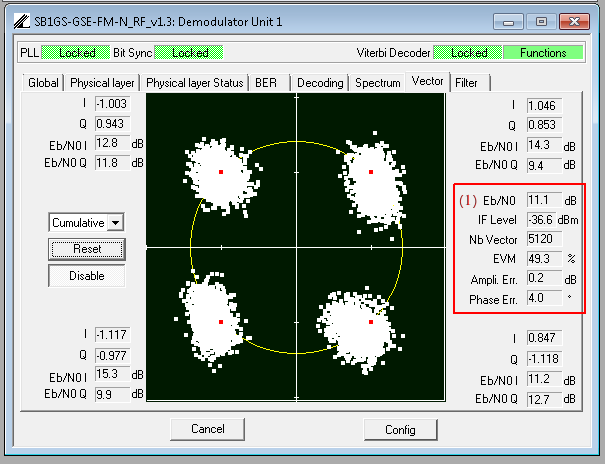
\includegraphics[width=0.4\textwidth]{figuras/SignalAnalysis.png}
	% 	\end{center}
	% 	\Extradetail
	% }
\SimpleExeStep{Adjust the Noise Power generation in Cortex HDR of TestBed in order to get
an Eb/N0 close to #2 in Cortex HDR of GS-GSE}
{Eb/N0  $\approx$  #2}
{\instring{dBm/Hz}{#1}{
    Go to Cortex HDR of RF TestBed and set an initial value of #1 in  Noise Level output, then adjust this, until obtain an Eb/N0 close to #2 in Cortex HDR of GS-GSE-FM.
}{
    Go to Cortex HDR of RF TestBed and adjust  Noise Level output until obtain Eb/N0 close to #2 in Cortex HDR of GS-GSE-FM.
}

In MCS Cortex (192.168.75.161) of  GS-GSE-FM (R), press Reset buttom and wait 20 seconds. Then, see Eb/N0 in the Vector tab of the DMU-1, in the Eb/N0 field (1)
\begin{center}
    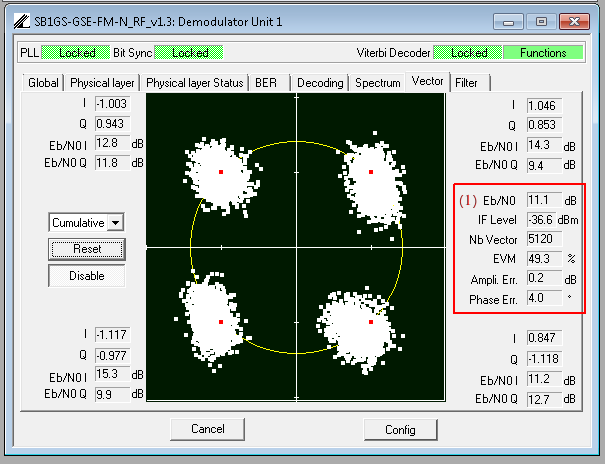
\includegraphics[width=0.4\textwidth]{figuras/SignalAnalysis.png}
\end{center}
\Extradetail}


}






% #endregion
% #region       ConnectFreqReferenceOfXbandUpconverterTestBed
\newcommand{\ConnectFreqReferenceOfXbandUpconverterTestBed}
{

\SimpleExeStep{	Connect reference of X-Band Upconverter of TestBed to time server. \tr{quiza este paso no vaya, no hace falta}}
{Reference connected}
{Connect the REF IN X-Band Upconverter (J5) to ref. J2 output Time Server of Lab using:
	\begin{minipage}[t]{\linewidth}
		\begin{itemize}[nosep,after=\strut]
			\item SBB4.18 cable.
			\item ATT10.11
			\item ATT1.11
		\end{itemize}
\end{minipage}}	
}

% #region       ConnectTestBedToGseNetwork
\newcommand{\ConnectTestBedToGseNetwork}[1]
{

\SimpleExeStep{Connect the RF TestBed to #1 network.}
{RF TestBed conected to #1 network.}
{Connect an ethernet free port of \textbf{Switch TestBed}  to  \textbf{\ethST{} \fmr} using a port in the range between 13 and 20
	or some free port of \textbf{\ethSD{}}.}

}
% #endregion
% #region       CopyConfigFileToCortexHDRTestBed
\newcommand{\CopyConfigFileToCortexHDRTestBed}[1]
{

\SimpleExeStep{Copy files for Noise generation to Cortex HDR of RF TestBed}
{File copied}
{	In the \comEgse{}, open the file explorer, and do the following:
	\begin{minipage}[t]{\linewidth}
		\begin{itemize}[nosep,after=\strut]
			\item Go to \\ C:/Users/EGSE COM/Documents/COMM-SS-FM/\sessionID/SB1FS-COM-D-011/cortex-testbed directory.
			\item Copy the file #1
			\item Connect to Cortex testbed with the following address and credentials:
			\begin{itemize}[nosep,after=\strut]
				\item Address: \bs{}\bs{}\hdrTBIP{}
				\item User: cortex
				\item Password: cortex
			\end{itemize}
			\item Go to to \bs{}\bs{}\hdrTBIP{}\bs{}zds\bs{}HDR\bs{}CrtxMCS\bs{}SABIA-Mar\bs{}AIT folder
			\item Paste the copied file.
		\end{itemize}
\end{minipage}}
}
% #endregion

% #region       CopyFileToCortexHDR
\newcommand{\CopyFileToCortexHDR}[1]
{
\SimpleExeStep{Copy files for BER measurement to Cortex HDR of #1}
{Files copied to cortex HDR}
{
	In the \comEgse{} do the following:
	\begin{minipage}[t]{\linewidth}
		\begin{itemize}[nosep,after=\strut]
			\item Open file explorer.
			\item Go to C:/Users/EGSE COM/Documents/COMM-SS-FM/\sessionID/SB1FS-COM-D-011/\allowbreak cortex-hdr.
			\item Copy the file \textbf{data52050}.
			\item Connect to Corte HDR with the following address and credentials:
			\begin{itemize}[nosep,after=\strut]
				\item Address: \bs{}\bs{}\hdrIP{}
				\item User: cortex
				\item Password: cortex
			\end{itemize}
			\item Go to \bs{}\bs{}\hdrIP{}\bs{}zds\bs{}HDR\bs{}SPS\bs{}BER\bs{} folder.
			\item Paste the copied file. If a file with the same name already exists, replace it.
		\end{itemize}
\end{minipage}}

}







%%%%%%%%%%%%%%%%%%%%%%%%%%%%%%%%%%%%%%%%%%%%%%%%%
% PXA
%%%%%%%%%%%%%%%%%%%%%%%%%%%%%%%%%%%%%%%%%%%%%%%%%
% #region       VerifyVsaRfInput
\newcommand{\VerifyVsaRfInput}
{
	
\SimpleExeStep{Verify RF hardware input for VSA}
{ThisAnalyzer9 input is selected.}
{In the menu VSA software of PXA do the following:
	\begin{minipage}[t]{\linewidth}
		\begin{itemize}[nosep,after=\strut]
			\item Click on the \textbf{Utilities, Hardware, Analyzer:Analyzer...} tabs.
		\end{itemize}
\end{minipage}}
}
% #endregion
% #region       ConnectDcBlockToPxa
\newcommand{\ConnectDcBlockToPxa}
{
\SimpleExeStep{Connect the DC Block to the RF input of PXA.}
{DC Block connected to PXA.}{Connect the DC Block to the RF input of the PXA.}
}

% #region       CheckHardDiskSpaceOnPxa
\newcommand{\CheckHardDiskSpaceOnPxa}
{
\SimpleExeStep{Check hard disk space on PXA}
{free space > 3 GB}
{On the PXA:
	\begin{minipage}[t]{\linewidth}
		\begin{itemize}[nosep,after=\strut]
			\item Launch the File Explorer.
			\item In the navigation panel on the left side of the folder, click "Computer."
			\item Check available storage space displayed under WINDOWS(D) drive.
		\end{itemize}
\end{minipage}}

}
% #endregion

% #region       VerifyDataModInPxa
\newcommand{\VerifyDataModInPxa}
{
    \stepcounter{Step}
    \immediate\write\myfile{|\theSec|\theStep|VerifyDataModInPxa|}
    \procedurestep{\theSec}{\theStep}{EXE}{Verify spectrum Data presence with the PXA.}
    {Spectrum present}{}{}
    \stepdetail{1}{0}{
        Observe the spectrum of the signal on the PXA. It must correspond to a carrier with modulation as shown in the following image:
        \begin{center}
            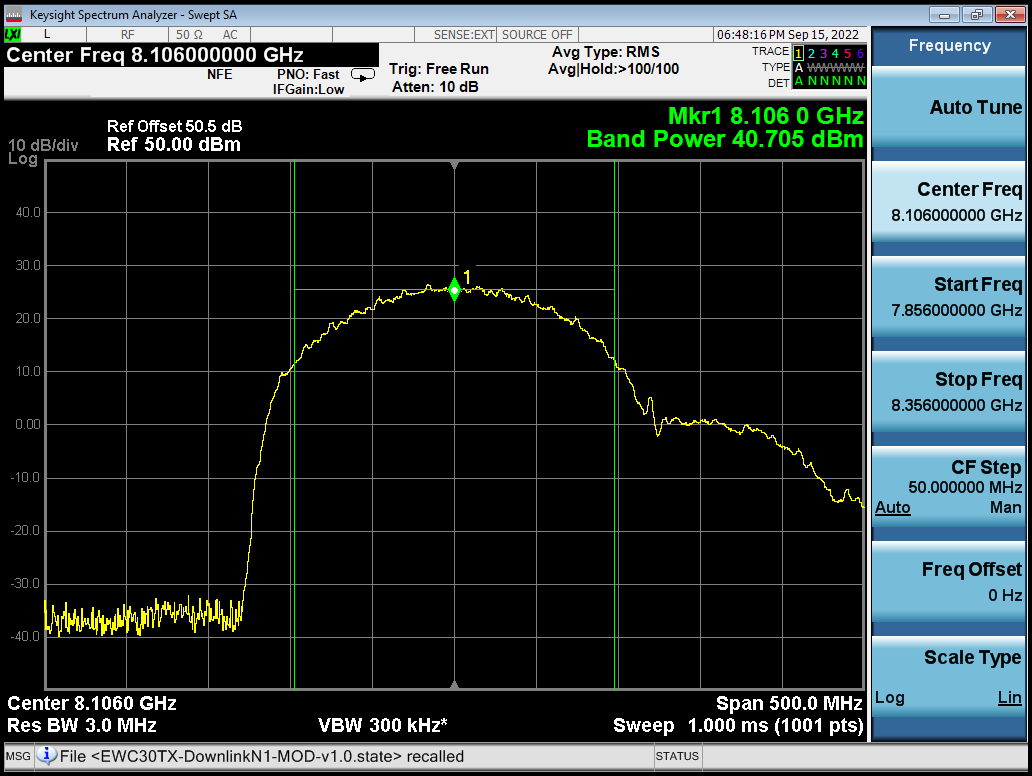
\includegraphics[width=0.6\textwidth]{figuras/data_mod.png}
        \end{center}
        \textbf{Note:} The image shown should be taken for illustrative purposes.

    }
}
% #endregion

% #region       TakeScreenShotOnPxaWithSingle{filename}
\newcommand{\TakeScreenShotOnPxaWithSingle}[1]
{
    \stepcounter{Step}
    \immediate\write\myfile{|\theSec|\theStep|TakeScreenShotOnPxaWithSingle|}
    \procedurestep{\theSec}{\theStep}{EXE}{Take screenshot of signals measurements.}{\texttt{#1} saved.}{\Result}{\Status}
    \stepdetail{}{}{
        \begin{minipage}[t]{\linewidth}
            \begin{itemize}[nosep,after=\strut]
                \item Press \textbf{Single} button.
                \item Press \textbf{Save} button.
                \item Press \textbf{Screen Image} key.
                \item Press \textbf{Save As} key.
                \item In the displayed window, select the \textbf{pxa-screenshot} folder in
                      \pxaTestFolderLocation{}\pxaTestFolderName{}\bs{}\procid{}\bs{}\allowbreak\subprocid{} directory.
                \item Enter file name: #1
                \item Press \textbf{Save} button.
                \item Press \textbf{Cont} button.
            \end{itemize}
        \end{minipage}
        \Extradetail
    }
}

% #region       TakeInitialScreenShotOnPxaWithSingle
\newcommand{\TakeInitialScreenShotOnPxaWithSingle}[1]
{
    \stepcounter{Step}
    \immediate\write\myfile{|\theSec|\theStep|TakeInitialScreenShotOnPxaWithSingle|}
    \procedurestep{\theSec}{\theStep}{EXE}{Take an initial screenshot in PXA before use Quick save button.}{\texttt{#1} saved.}{\Result}{\Status}
    \stepdetail{}{}{
        \begin{minipage}[t]{\linewidth}
            \begin{itemize}[nosep,after=\strut]
                \item Press \textbf{Single} button.
                \item Press \textbf{Save} button.
                \item Press \textbf{Screen Image} key.
                \item Press \textbf{Save As} key.
                \item In the displayed window, browse to the
                      \textbf{\pxaTestFolderLocation{}\pxaTestFolderName{}\bs{}\procid{}\bs\subprocid{}\bs{pxa-screenshot}} directory.
                \item Enter File Name: #1.
                \item Press \textbf{Save} button.
                \item Press \textbf{Cont} button.
            \end{itemize}
        \end{minipage}
        \textbf{Note:} When pressing QuickSave button a new <file name>\_nnnn.png screenshot is saved. nnnn start from 0 and increase every quick save.
        \Extradetail
    }
}

% #region       TakeInitialScreenShotOnPxa
\newcommand{\TakeInitialScreenShotOnPxa}[1]
{
    \stepcounter{Step}
    \immediate\write\myfile{|\theSec|\theStep|TakeInitialScreenShotOnPxa|}
    \procedurestep{\theSec}{\theStep}{EXE}{Take an initial screenshot in PXA before use Quick save button.}{\texttt{#1} saved.}{\Result}{\Status}
    \stepdetail{}{}{
        \begin{minipage}[t]{\linewidth}
            \begin{itemize}[nosep,after=\strut]
                \item Press \textbf{Save} button.
                \item Press \textbf{Screen Image} key.
                \item Press \textbf{Save As} key.
                \item In the displayed window, browse to the
                      \textbf{\pxaTestFolderLocation{}\bs{}\pxaTestFolderName{}\allowbreak\bs{}\procid{}\bs\subprocid{}\bs{pxa-screenshot}} directory.
                \item Enter File Name: #1.
                \item Press \textbf{Save} button.
            \end{itemize}
        \end{minipage}
        \textbf{Note:} When pressing QuickSave button a new <file name>\_nnnn.png screenshot is saved. nnnn start from 0 and increase every quick save.
        \Extradetail
    }
}

% #endregion


% #region       MeasureCCDFWithPxa{10.0 M/10.0 Mpt}}
\newcommand{\MeasureCCDFWithPxa}[1]
{
    \stepcounter{Step}
    \immediate\write\myfile{|\theSec|\theStep|MeasureCCDFWithPxa|}
    \procedurestep{\theSec}{\theStep}{EXE}{Measure CCDF using PXA.}{CCDF measured}{\Result}{\Status}
    \stepdetail{1}{0}{On PXA instrument:
        \begin{minipage}[t]{\linewidth}
            \begin{itemize}[nosep,after=\strut]
                \item Press Restart button to make a fresh measurement.
                \item Wait until the Counts: \textbf{#1} indicator (See image below)  is complete.
            \end{itemize}
        \end{minipage}
        \begin{center}
            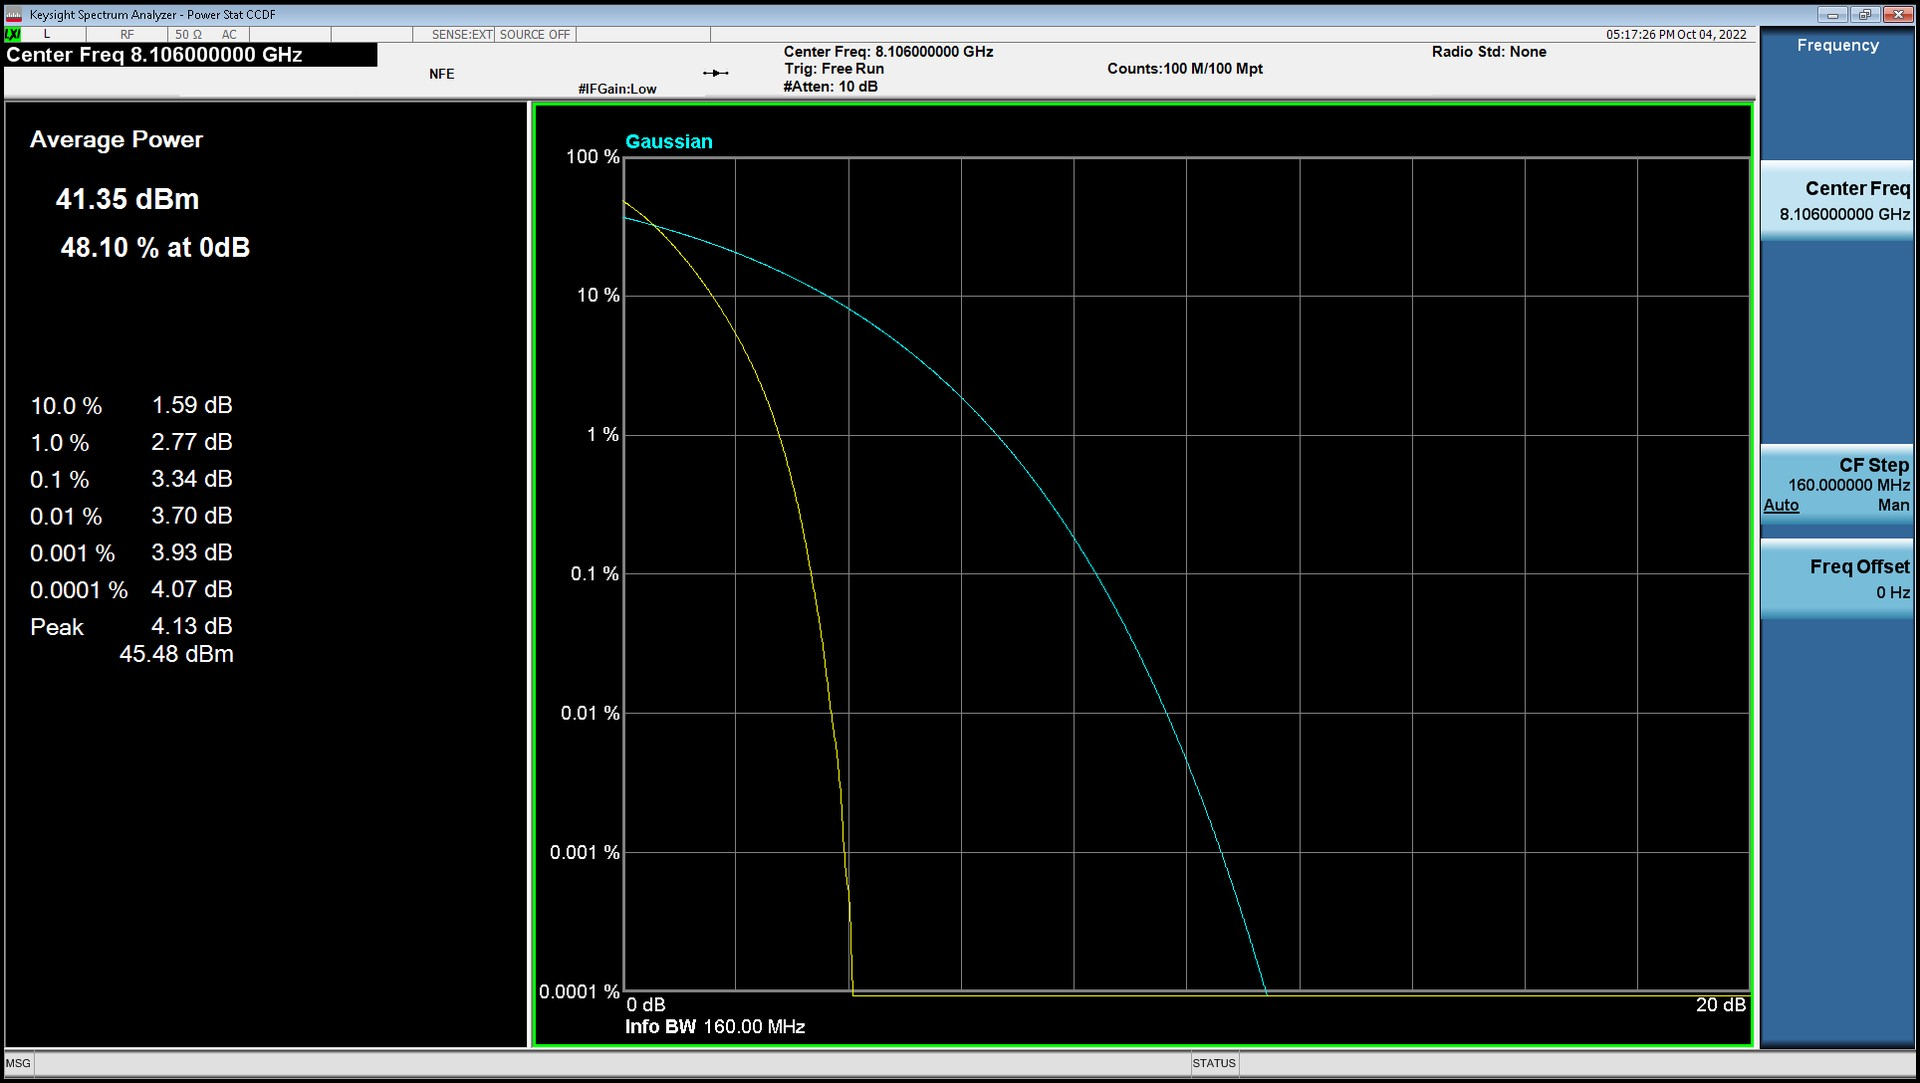
\includegraphics[width=0.53\textwidth]{figuras/DATA-CCDF.png}
        \end{center}
        \textbf{Note:} The image shown should be taken for illustrative purposes.

    }
}
% #endregion
% #region       MeasureCHpowerWithPxa{100 M/100 Mpt}}
\newcommand{\MeasureCHPowerWithPxa}[1]
{
    \stepcounter{Step}
    \immediate\write\myfile{|\theSec|\theStep|MeasureCHPowerWithPxa|}
    \procedurestep{\theSec}{\theStep}{EXE}{Measure channel power using PXA.}{P = 40 dBm +/- 1dB}{\Result}{\Status}
    \stepdetail{1}{0}{On PXA instrument:
        \begin{minipage}[t]{\linewidth}
            \begin{itemize}[nosep,after=\strut]
                %\item Press Restart button to make a fresh measurement.
                \item Wait until the Counts: \textbf{#1} indicator (See image below)  is complete.
                \item Verify that the measurement meets the expected value.
            \end{itemize}
        \end{minipage}
        \begin{center}
            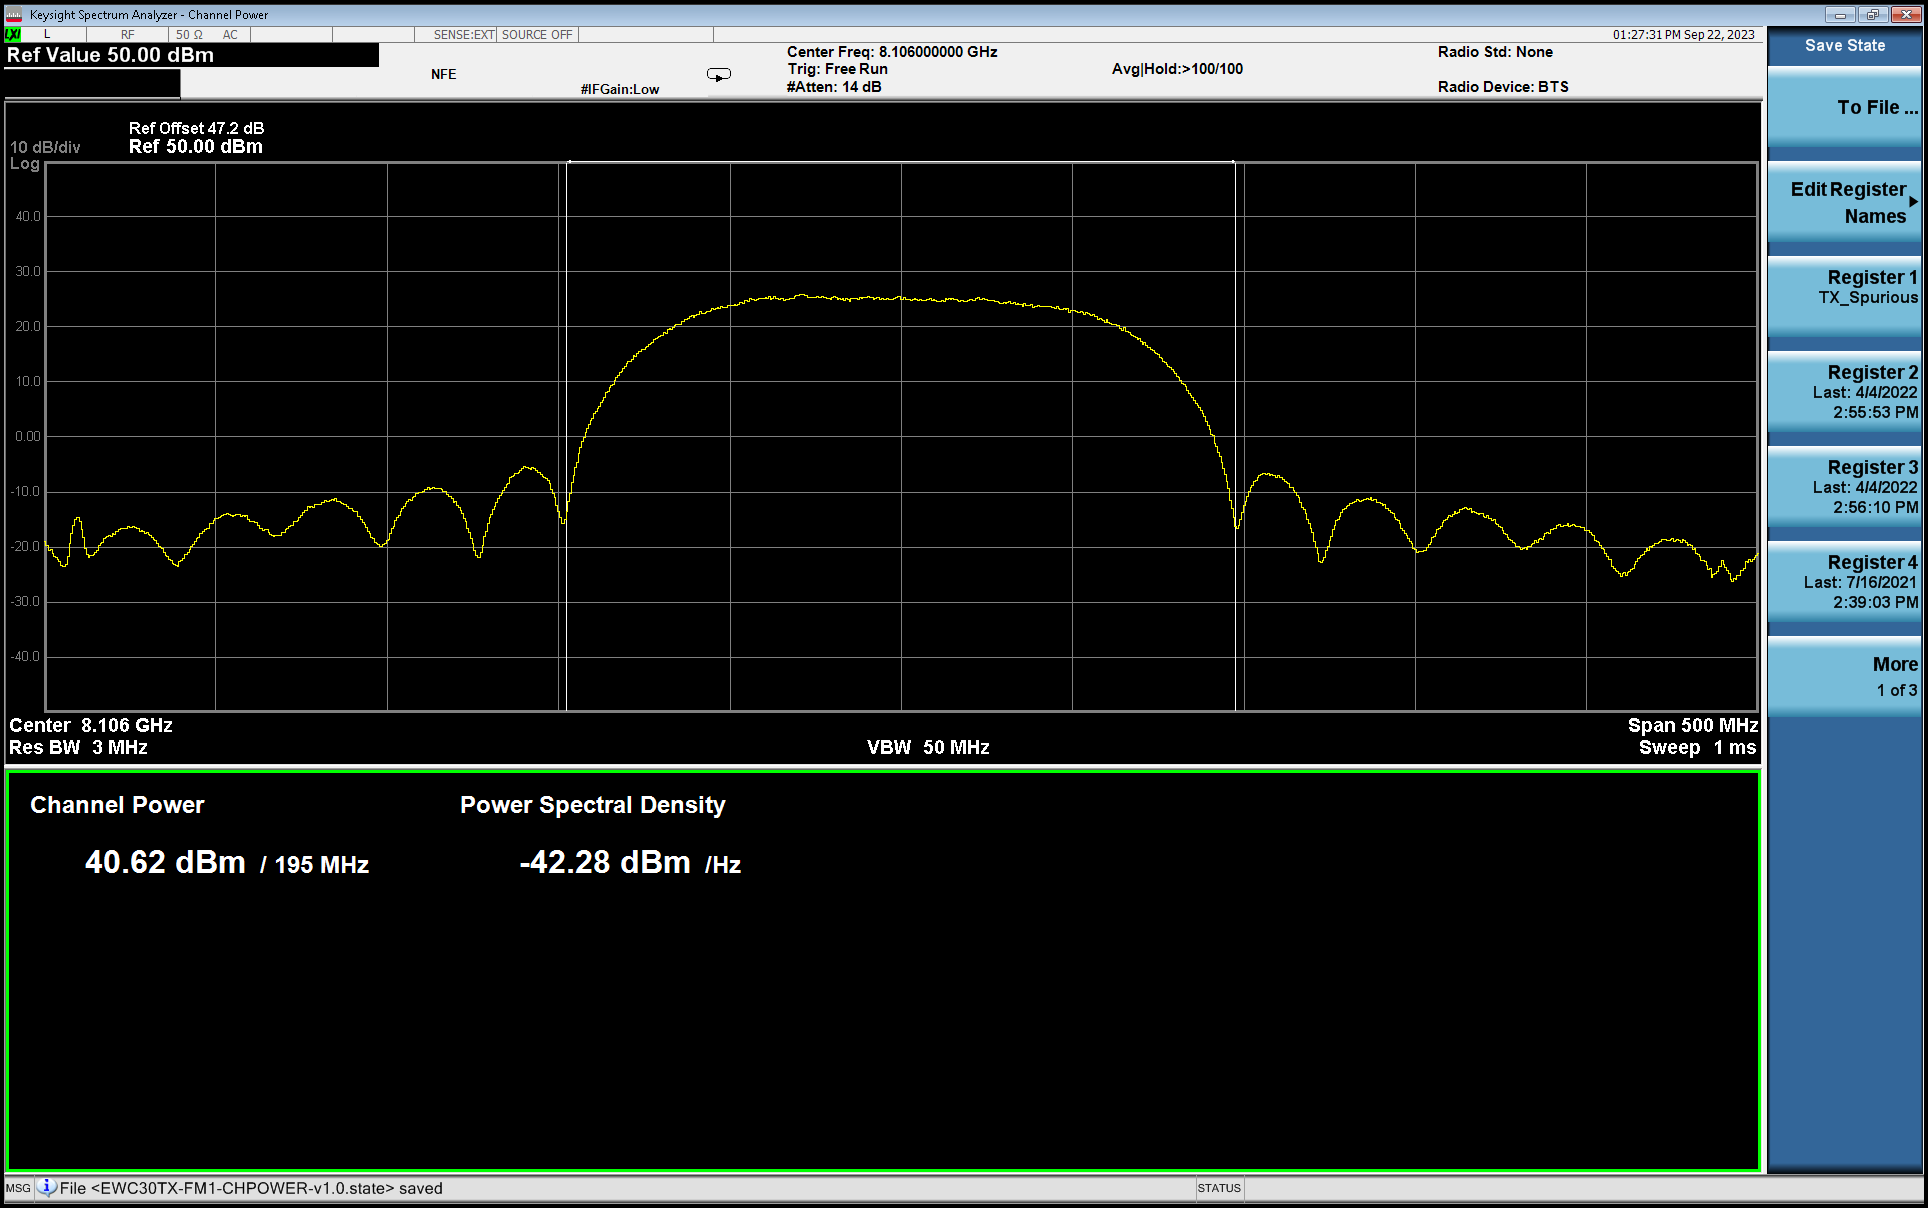
\includegraphics[width=0.53\textwidth]{figuras/CHPower.png}
        \end{center}
        \textbf{Note:} The image shown should be taken for illustrative purposes.
    }
}
% #endregion

% #region       MeasureOBWWithPxa{100 M/100 Mpt}}
\newcommand{\MeasureOBWAndFreqWithPxa}[1]
{
    \stepcounter{Step}
    \immediate\write\myfile{|\theSec|\theStep|MeasureOBWAndFreqWithPxa|}
    \procedurestep{\theSec}{\theStep}{EXE}{Measure OBW and frequency error using PXA.}{OBW $\approx$ 205 MHz\\ Freq error < 500 KHz}{\Result}{\Status}
    \stepdetail{1}{0}{On PXA instrument:
        \begin{minipage}[t]{\linewidth}
            \begin{itemize}[nosep,after=\strut]
                %\item Press Restart button to make a fresh measurement.
                \item Wait until the Counts: \textbf{#1} indicator (See image below)  is complete.
                \item Verify that the OBW and Transmit Freq Error meets the expected value. The displayed Freq Error is the difference between the value configured in the PXA 
                and the measured value.
            \end{itemize}
        \end{minipage}
        \begin{center}
            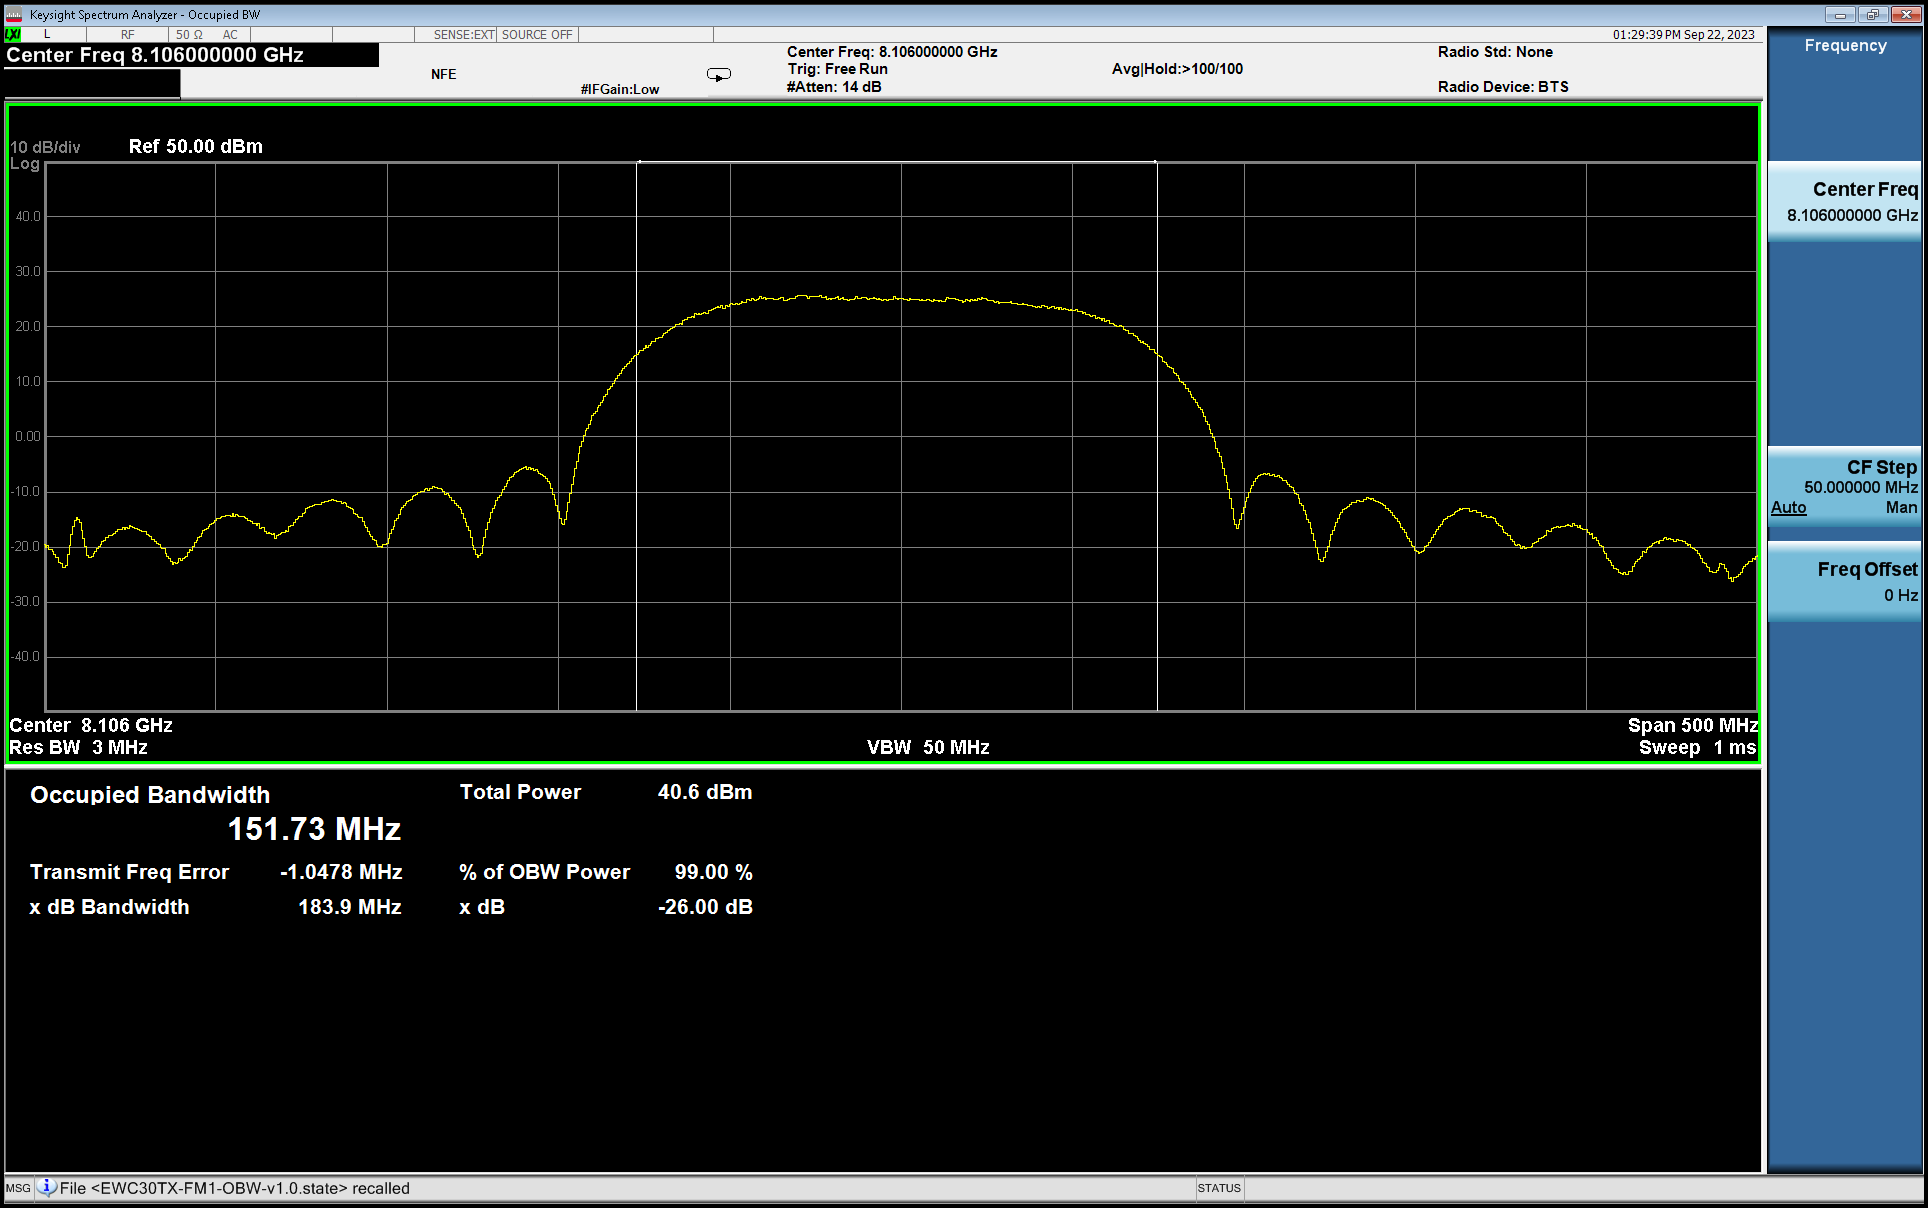
\includegraphics[width=0.53\textwidth]{figuras/OBW.png}
        \end{center}
        \textbf{Note:} The image shown should be taken for illustrative purposes.

    }
}
% #endregion






% #region       MeasureCarrierPowerAndFreqUsingPxaEveryMinute
\newcommand{\MeasureCarrierPowerAndFreqUsingPxaEveryMinute}
{
    \stepcounter{Step}
    \immediate\write\myfile{|\theSec|\theStep|MeasureCarrierPowerAndFreqUsingPxaEveryMinute|}
    \procedurestep{\theSec}{\theStep}{EXE}{Measure carrier power and frequency every 60 seconds during temperature stabilization.}{measurements performed}{\Result}{\Status}
    \stepdetail{1}{0}{On PXA instrument:
        \begin{minipage}[t]{\linewidth}
            \begin{itemize}[nosep,after=\strut]
                \item Press \textbf{Restart} button when PXA clock time ends in 00 seconds.
                \item Press \textbf{Quick Save} button when PXA clock time ends in 40 seconds.
                \item Register PXA screenshot file name in table \ref{tb:freqstab}.
                \item Register \textbf{O\_TX\_TEMPERATURE} in table  \ref{tb:freqstab}.
                \item Repeat until Tx temperature remains stable for 5 minutes.
            \end{itemize}
        \end{minipage}
    }
  }






% #region       SaveTraceOnPxaPN
\newcommand{\SaveTraceOnPxaPN}[1]
{
    \stepcounter{Step}
    \immediate\write\myfile{|\theSec|\theStep|SaveTraceOnPxaPN|}
    \procedurestep{\theSec}{\theStep}{EXE}{Save trace #1 of phase noise measurement.}{\texttt{#1.csv} saved.}{\Result}{\Status}
    \stepdetail{}{}{
        \begin{minipage}[t]{\linewidth}
            \begin{itemize}[nosep,after=\strut]
                \item Press \textbf{Save} button.
                \item Press \textbf{Data (Export)} key.
                \item Press \textbf{Trace} key.
                \item Press \textbf{Trace #1} key.
                \item Press \textbf{Save as ...} key.
                \item In the displayed window, select the \textbf{pxa-trace} folder in
                      \pxaTestFolderLocation\bs{}\pxaTestFolderName\bs{}\procid{}\bs{}\subprocid{} directory.
                \item Enter as file name: #1.csv
                \item Press \textbf{Save} button.
            \end{itemize}
        \end{minipage}
        \Extradetail
    }
}
% #endregion


% #region       SaveTraceOnPxaPhaseNoiseMode
\newcommand{\SaveTraceOnPxaPhaseNoiseMode}
{
    \stepcounter{Step}
    \immediate\write\myfile{|\theSec|\theStep|SaveTraceOnPxaPhaseNoiseMode, \pxaTestFolderLocation{}\pxaTestFolderName{}\string\ \procid{}\string\ \subprocid{}\string\ pxa-screenshot|}
    \procedurestep{\theSec}{\theStep}{EXE}{Take trace of signals measurements.}{\texttt{<filename.trace>} saved.}{\Result}{\Status}
    \stepdetail{}{}{
        \begin{minipage}[t]{\linewidth}
            \begin{itemize}[nosep,after=\strut]
                \item Press \textbf{Save} button.
                \item Press \textbf{Data (Export) Trace 1} key.
                \item Press \textbf{Save As} key.
                \item In the displayed window, select the \textbf{pxa-screenshot} folder in
                      \pxaTestFolderLocation{}\pxaTestFolderName{}\bs\procid{}\bs\subprocid{} directory.
                \item Press \textbf{Save} button.
                \item Take note of the saved file name.
            \end{itemize}
        \end{minipage}
        \Extradetail
    }
}
% #endregion

% #region       SaveCSVOnPxaCCDFMode
\newcommand{\SaveCSVOnPxaCCDFMode}[1]
{
    \stepcounter{Step}
    \immediate\write\myfile{|\theSec|\theStep|SaveCSVOnPxaCCDFMode|}
    \procedurestep{\theSec}{\theStep}{EXE}{Save CSV of signals measurements.}{\texttt{#1} saved.}{\Result}{\Status}
    \stepdetail{}{}{
        \begin{minipage}[t]{\linewidth}
            \begin{itemize}[nosep,after=\strut]
                \item Press \textbf{Save} button.
                \item Press \textbf{Data (Export)} key.
                \item Select \textbf{Meas Result} option.
                \item Press \textbf{Save As...} key.
                \item In the displayed window, select the \textbf{pxa-trace} folder in
                      \pxaTestFolderLocation{}\pxaTestFolderName{}\bs{}\procid{}\bs{}\allowbreak\subprocid{} directory.
                \item Enter the file name: #1.
                \item Press \textbf{Save} button.
            \end{itemize}
        \end{minipage}
        \Extradetail
    }
}
% #endregion


% #region       ChangeTxStatusToXBand{Mode}{M|R}
\newcommand{\ChangeTxStatusToXBand}[3]
{
    \ifstrequal{#2}{M}{}{
    \ifstrequal{#2}{R}{}{
        \errmessage{expected M or R}
    }}

    \stepcounter{Step}
    \immediate\write\myfile{|\theSec|\theStep|ChangeTxStatusToXBand,STATUS=#1, SIZE=#2|}
    \ifstrequal{#1}{Standby}{
        \procedurestep{\theSec}{\theStep}{EXE}
        {Send command \textbf{I\_OPE\_2\_STBY\_#2} to change Tx status to Standby Mode.}
        {\textbf{Standby Mode} indicator is ON}{\Result}{\Status}
        \stepdetail{1}{0}{#3
        Go to HV-HPC tab on \comEgse{} GUI and press \textbf{I\_OPE\_2\_STBY\_#2} button. Button turns green during 0.6 seconds.\\ Verify Tx Status in \textbf{STATE} section of \comEgse{} GUI.
        }
    }{
    \ifstrequal{#1}{Operational}{
        \procedurestep{\theSec}{\theStep}{EXE}
        {Send command \textbf{I\_STBY\_2\_OPE\_#2} to change Tx status to Operational Mode.}
        {\textbf{Operation Mode} indicator is ON}{\Result}{\Status}
        \stepdetail{1}{0}{#3
        Go to HV-HPC tab on \comEgse{} GUI and press \textbf{I\_STBY\_2\_OPE\_#2} button. Button turns green during 0.6 seconds.\\ Verify Tx Status in \textbf{STATE} section of \comEgse{} GUI.
        }
    }{
        \errmessage{Expected Standby or Operational}
    }}
}


% #region       DeletePxaScreenShotsOnPxa
\newcommand{\DeletePxaScreenShotsOnPxa}
{
    \stepcounter{Step}
    \immediate\write\myfile{|\theSec|\theStep|DeletePxaScreenShotsOnPxa}
    \procedurestep{\theSec}{\theStep}{EXE}{Delete evidences folder in the PXA.}{Folder deleted.}{\Result}{\Status}
    \stepdetail{1}{0}{
        In the \comEgse{}, open the file explorer, connect to PXA with the following address and credentials:
        \begin{minipage}[t]{\linewidth}
            \begin{itemize}[nosep,after=\strut]
                \item Address: \texttt{\bs{}\bs{}\pxaIP{}\bs{}}
                \item User: administrator
                \item Password: agilent4u
            \end{itemize}
        \end{minipage}
        and do the following:
        \begin{minipage}[t]{\linewidth}
            \begin{itemize}[nosep,after=\strut]
                \item Go to \bs{}\bs{}\pxaIP{}\bs{}\pxaTestFolderLocation{}\pxaTestFolderName{}\procid{}\bs{}\subprocid{} directory.
                \item Select all the content and delete it by pressing SHIFT+DEL keys.
            \end{itemize}
        \end{minipage}
        \Extradetail
    }
}

% #region       MeasurePhaseNoiseDANLWithPxa
\newcommand{\MeasurePhaseNoiseDANLWithPxa}
{
    \stepcounter{Step}
    \immediate\write\myfile{|\theSec|\theStep|MeasurePhaseNoiseDANLWithPxa|}
    \procedurestep{\theSec}{\theStep}{EXE}{Measure DANL with the PXA.}{DANL saved in trace3}{\Result}{\Status}
    \stepdetail{1}{0}{On PXA instrument:
        \begin{minipage}[t]{\linewidth}
            \begin{itemize}[nosep,after=\strut]
                \item Press \textbf{Restart} button to make a first carrier acquisition.
                \item Press \textbf{MeasSetup} button.
                \item Press \textbf{Meas type} key and select \textbf{DANL floor}.
                \item Press \textbf{Restart} button.
                \item Press \textbf{trace/detector} button and select \textbf{More/Copy Echange} keys.
                \item Select From \textbf{Trace 2} to \textbf{Trace 3}.
                \item Press \textbf{From Trace} key and select \textbf{Trace 2}
                \item Press \textbf{To Trace} key and select \textbf{Trace 3}
                \item Press \textbf{Copy Now} key.
                \item Press \textbf{MeasSetup} button.
                \item Press \textbf{Meas type} key and select \textbf{Phase Noise}.
            \end{itemize}
        \end{minipage}
        %\begin{center}
        %    \includegraphics[width=0.53\textwidth]{figuras/phase_noise_meas.png}
        %\end{center}
    }
}
% #endregion

% #region       MeasurePhaseNoiseWithPxa
\newcommand{\MeasurePhaseNoiseWithPxa}
{
    \stepcounter{Step}
    \immediate\write\myfile{|\theSec|\theStep|MeasurePhaseNoiseWithPxa|}
    \procedurestep{\theSec}{\theStep}{EXE}{Measure Phase Noise using PXA.}{$phase\ noise\ <\ 6^o{rms}$}{\Result}{\Status}
    \stepdetail{1}{0}{On PXA instrument:
        \begin{minipage}[t]{\linewidth}
            \begin{itemize}[nosep,after=\strut]
                \item Press \textbf{Restart} button to make a fresh measurement.
                \item Wait until measurement ends. The observed measurement should be similar to the figure below.
                \item Verify that the measured value is as expected.
                      %\item Press Quick Save button.
            \end{itemize}
        \end{minipage}
        \begin{center}
            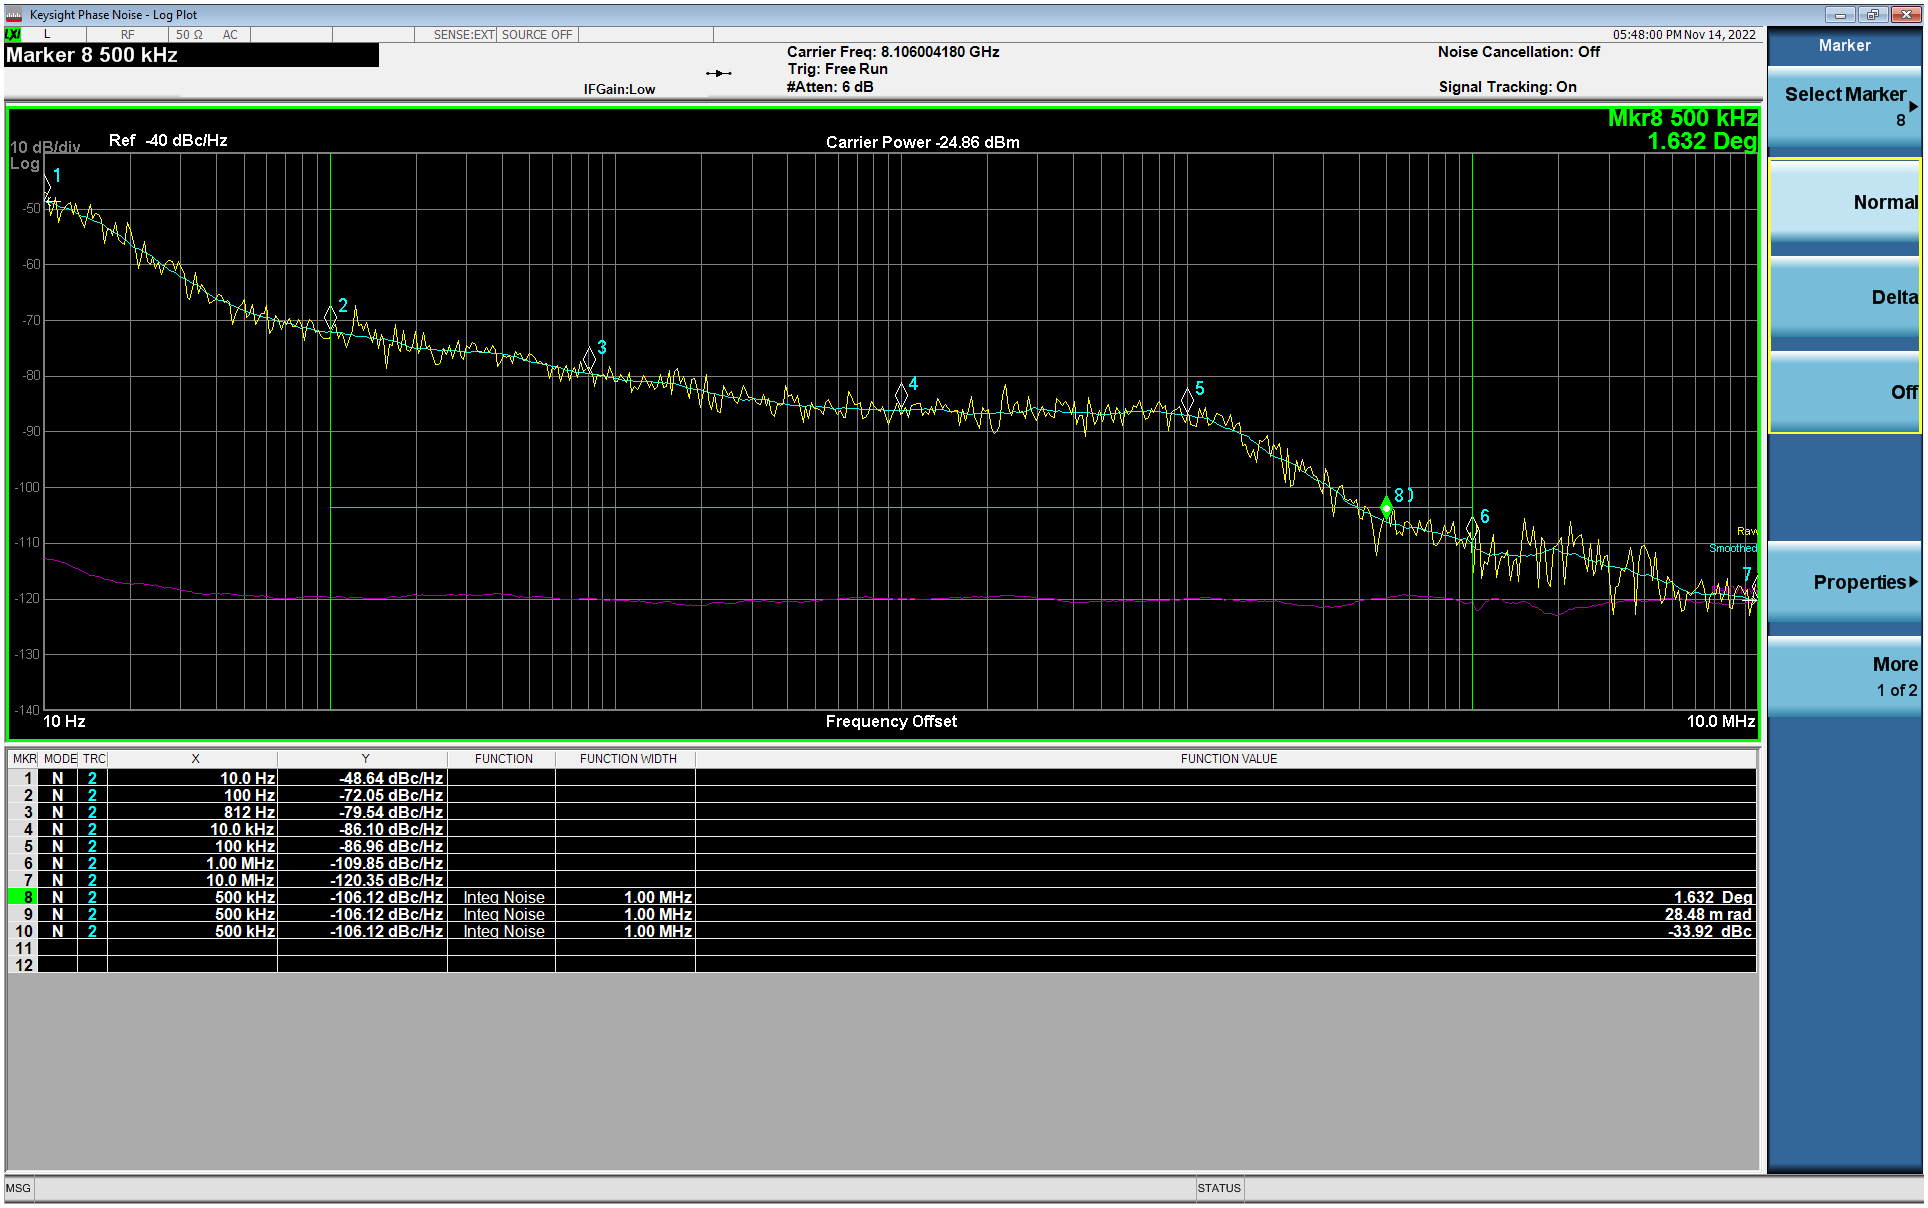
\includegraphics[width=0.53\textwidth]{figuras/data-lol-phase-noise.png}
        \end{center}
        \textbf{Note:} The image shown should be taken for illustrative purposes.

    }
}
% #endregion
%%%%%%%%%%%%%%%%%%%%%%%%%%%%%%%%%%%%%%%%%%%%%%%%%%%%%%%%%%%%%%%%%%%%%%%%
% Macros para ensayo de filtro
%%%%%%%%%%%%%%%%%%%%%%%%%%%%%%%%%%%%%%%%%%%%%%%%%%%%%%%%%%%%%%%%%%%%%%%%

\newcommand{\foldername}{folder name}
% #region       OpenMcsWindowsInCortexHdrGseForFilterTuninglTest{Folder Name}
\newcommand{\OpenMcsWindowsInCortexHdrGseForFilterTuninglTest}
{
    \stepcounter{Step}
    \procedurestep{\theSec}{\theStep}{EXE}{Open Global, Spectrum and Vector plots in Cortex HDR of GS-GSE-FM (R).}{Windows open.}{}{}
    \stepdetail{1}{0}{
Go to MCS Cortex (192.168.75.161). According to the figures below, do the following:
        \begin{minipage}[t]{\linewidth}
            \begin{itemize}[nosep,after=\strut]
                \item Global tab of DMU-1 (Demodulator Unit 1):
                \begin{itemize}
                    \item In the Global window, click on the DMU-1.
                    \item In the displayed window go to Global tab. 
                \end{itemize}
                \item Spectrum tab of DMU-1:
                \begin{itemize}
                    \item In the Global window, click on the DMU-1.
                    \item In the displayed window go to Spectrum tab and press enable button.
                \end{itemize}
                \item Vector tab of DMU-1:
                \begin{itemize}
                    \item In the Global window, click on the DMU-1.
                    \item In the displayed window go to vector tab, select cumulative option and press enable button.
                \end{itemize}
                \item Global tab of DRU-1:
                \begin{itemize}
                    \item In the Global window, click on the DRU-1 (Data Recording Unit 1).
                    \item In the displayed window go to Global tab.
                \end{itemize}
            \end{itemize}
        \end{minipage}
        \begin{center}
            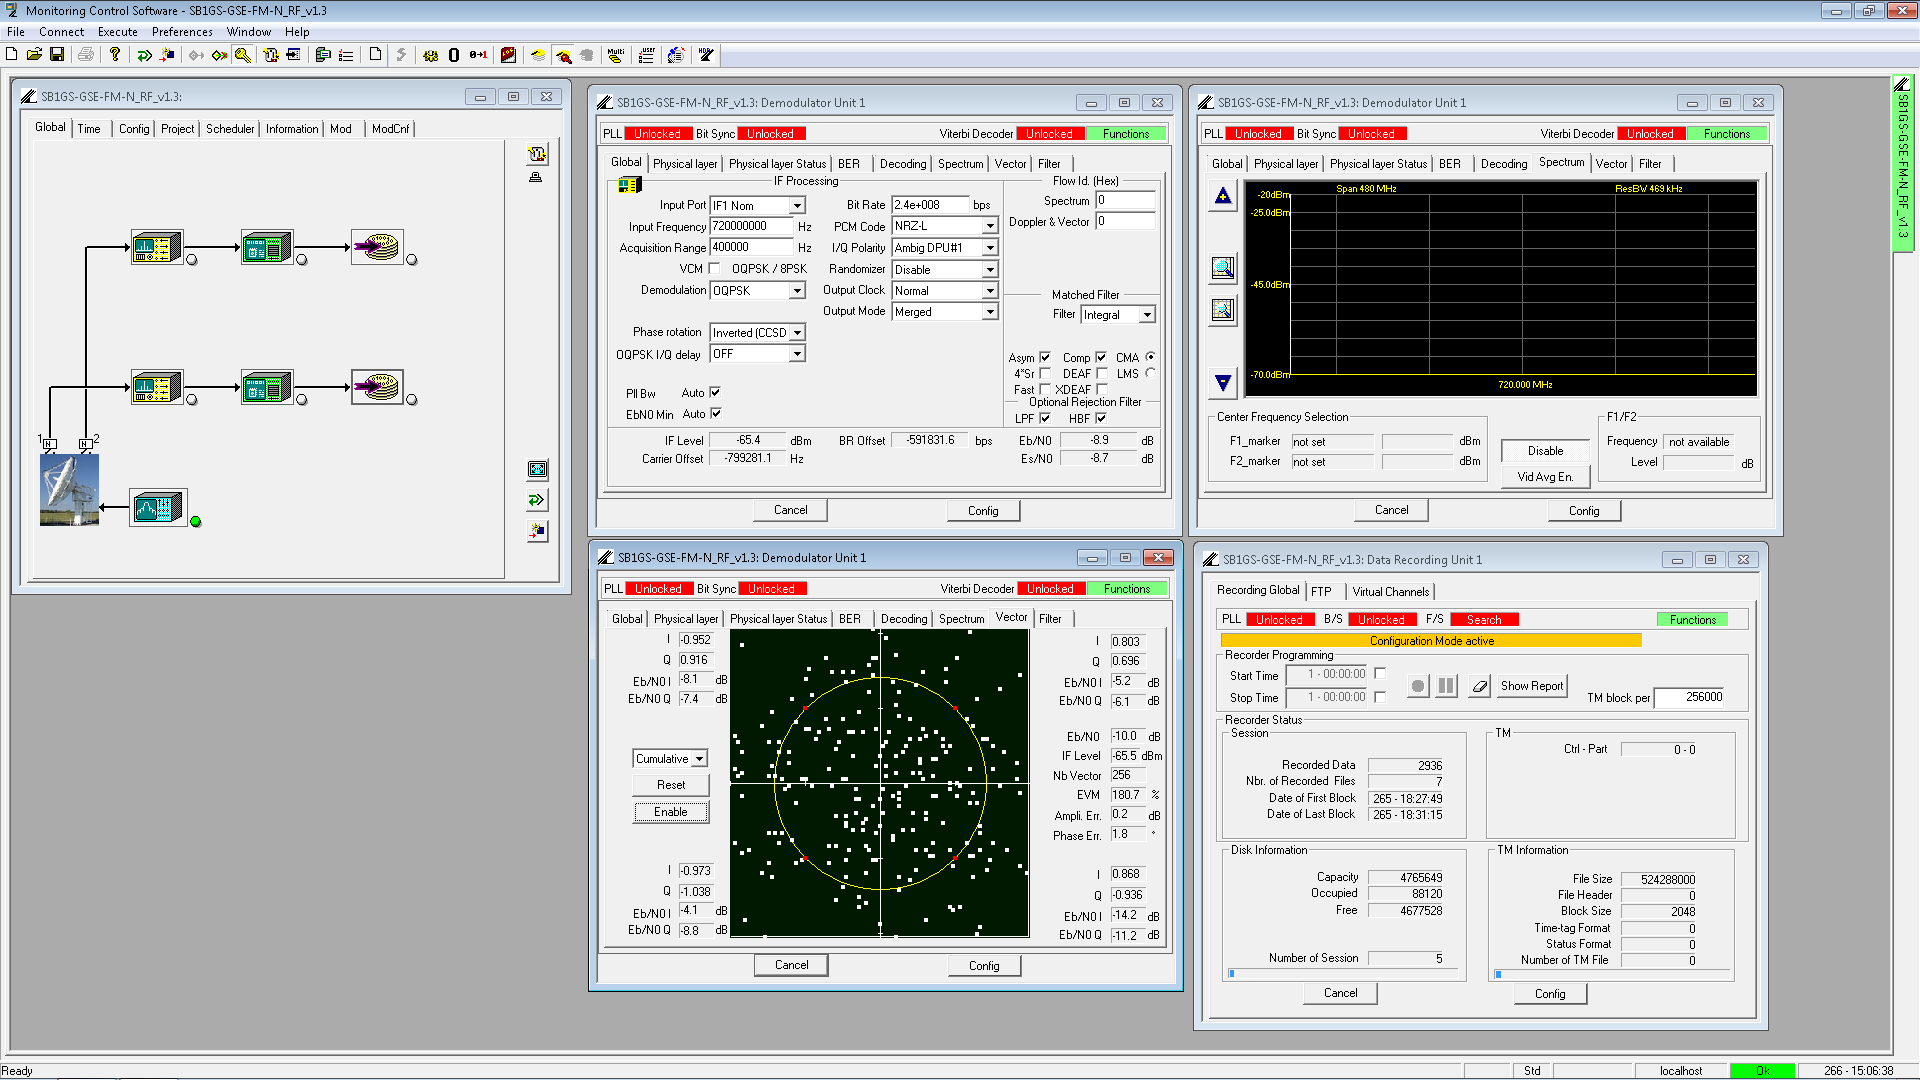
\includegraphics[width=0.53\textwidth]{figuras/cortex-hdr-filter-tuning.png}
        \end{center}  
        \textbf{Note:} The image shown should be taken for illustrative purposes.
 
    }
}

% #region       VerifyMatchedFilterParametersInCortexHdrGse{Folder Name}
\newcommand{\VerifyMatchedFilterParametersInCortexHdrGse}
{
    % Step - Crear carpeta de capturas en cortex
    \stepcounter{Step}
    \procedurestep{\theSec}{\theStep}{EXE}{
Verify Matched Filter parameter of Cortex HDR of GS-GSE-FM (R).
}{
Matched Filter -> Filter = RootRaised filter\\
Roll-Off = 0.5\\
Matched Filter -> Asym, Comp, DEAF, LMS, LPF and HBF checked
}{}{}
    \stepdetail{1}{0}{
Go to MCS Cortex (192.168.75.161), in Global tab of DMU-1 (Demodulator Unit 1), verify the following:
        \begin{minipage}[t]{\linewidth}
            \begin{itemize}[nosep,after=\strut]
                \item Matched Filter -> Filter = RootRaised filter
                \item Roll-Off = 0.5
                \item Matched Filter -> Asym, Comp, DEAF, LMS checked
                \item Optional Rejection Filter -> LPF and HBF checked
            \end{itemize}
        \end{minipage}                
    }
}

% #region       SetCegseVariableAttenuatorTo
\newcommand{\SetCegseVariableAttenuatorTo}[2]
{
    \stepcounter{Step}
    \immediate\write\myfile{|\theSec|\theStep|SetCegseVariableAttenuatorTo|}
    \procedurestep{\theSec}{\theStep}{EXE}{Set \textbf{#1 step Variable Attenuator} in CEGSE to #2.}{Attenuation in #2.}{\Result}{\Status}
    \stepdetail{1}{0}{Set \textbf{#1 step Variable Attenuator} in CEGSE to #2 attenuation position.\\\Extradetail}
}
% #endregion

% #region       SendStoredFileWithDurationXBand{File name}{HV-HPC Command}
\newcommand{\SendStoredFileWithDurationXBand}[3]
{
    \stepcounter{Step}
    \immediate\write\myfile{|\theSec|\theStep|SendStoredFileWithDurationXBand, FILE:\comEgseTestFolderLocation{}\comEgseTestFolderName{}\string\ \sessionID\string\ \procid{}\string\ \subprocid{}\string\ #1 CMD:#2|}
    \procedurestep{\theSec}{\theStep}{EXE}{Start data transmission for #3}{Data transmission started}{\Result}{\Status}
    \stepdetail{1}{0}{
        In the \comEgse{}{} SW:
        \begin{minipage}[t]{\linewidth}
            \begin{itemize}[nosep,after=\strut]
                \item Got to the \textbf{COMM} tab and then go to the \textbf{Downlink} subtab.
                \item Verify that “stage” box does not show "Sending X-Band File" message.
                \item On the \textbf{Stored Downlink File} box choose the file \texttt{#1} in
                      \texttt{\comEgseTestFolderLocation{}\comEgseTestFolderName{}\bs{}\sessionID\bs{}\procid{}\bs{}} directory.
                \item Switch file selector to \textbf{Send Stored Downlink File}
                \item Place the switch in "#2"
                \item Switch \textbf{Bit Endianness} selector to \textbf{Big}.
                \item Press \textbf{Send} button.
                \item Verify that “stage” box shows \textbf{Sending X Band File}.
            \end{itemize}
        \end{minipage}
\textbf{Note:} The transmission time of the EWC30 is #3, if it ends before all mesurements are performed transmit againg when EWC30 temperature is low.\\
\textbf{Note:} Constantly check the temperature, if it is higher than 53°C switch the EWC30 to standby mode (by pressing I\_OPE\_2\_STBY\_M in HV-HPC tab) and wait until it cools down. Then repeat this step and resume test execution.
        \Extradetail
    }
}
% #endregion

% #region       MeasureRfDataCharacteristicsOnVSA
\newcommand{\MeasureRfDataCharacteristicsOnVSA}[1]
{
    \stepcounter{Step}
    \immediate\write\myfile{|\theSec|\theStep|MeasureRfDataCharacteristicsOnVSA|}
    \procedurestep{\theSec}{\theStep}{EXE}{
        Measure Data characteristics in VSA}{
        - Freq Err {$<\ 500KHz$} \\
        - EVM [\%] \\
        - Mag Err [\%]\\ 
        - Phase Err [°]\\
        - Output power = #1\\% de portadora hay que tener unamedicion de lapotencia de la señal modulada al a entrada del GSE para hacer el calculo de elnace\\
        %- Ocupied bandwidth  $\leq 162\ 000\ 000\ Hz.$\\ % decalculado usando (R/n)*(1+alfa)
        - Modulation scheme = $O-QPSK(4\ states).$\\
       }{\Result}{\Status}
    \stepdetail{1}{0}{According to the image below, do the following:
        \begin{minipage}[t]{\linewidth}
            \begin{itemize}[nosep,after=\strut]
                \item In window D (QPSK Syms/Errs), verify that \textbf{Freq Err} meets the expected values (1), 
                the displayed Freq Err is the difference between the value configured in the VSA 
                software and the measured value. Take note of the measured values of \textbf{EVM}, \textbf{Mag Err} and \textbf{Phase Err}.
                \item In window B (Ch1: Spectrum), verify that the \textbf{output power} meets the expected values (2).
                \item In window A (QPSK Meas Time), verify that the \textbf{modulation scheme} is as expected.
                %\item In the Markers window, verify that the \textbf{ocupied bandwidth} meets the expected values (3).
            \end{itemize}
        \end{minipage}
        \begin{center}
            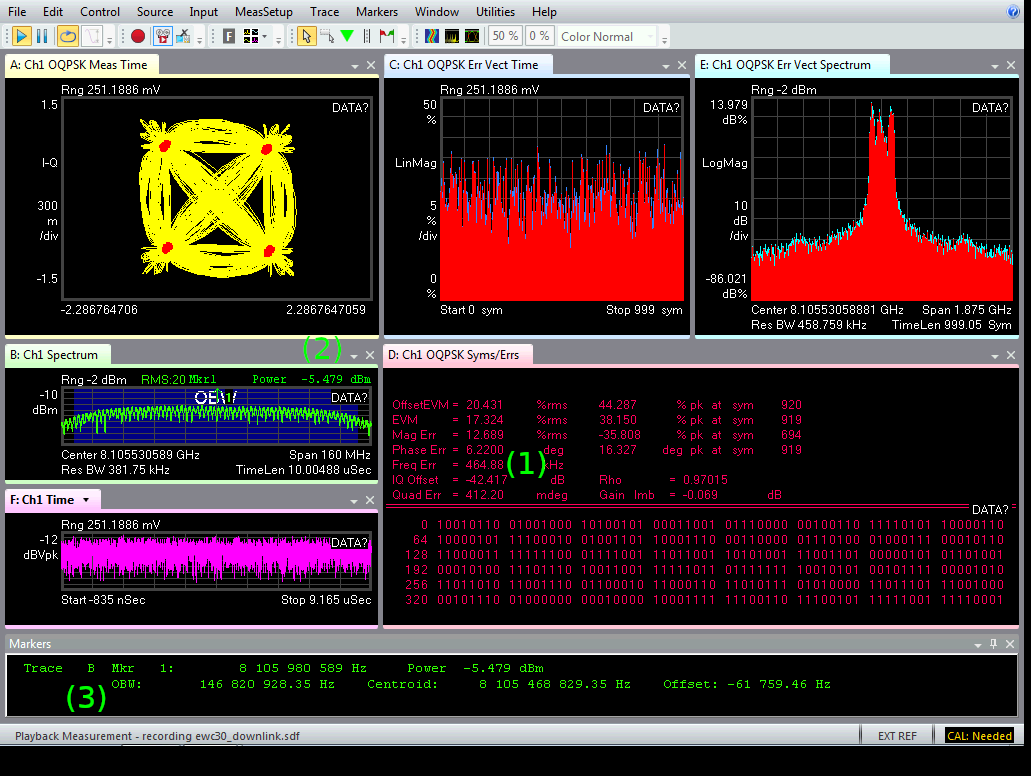
\includegraphics[width=0.41\textwidth]{figuras/downlink_EWC30.png}
        \end{center}
        \Extradetail
    }
}
% #endregion

% #region       RestartIFRInCortexHdr
\newcommand{\RestartIFRInCortexHdr}[1]
{
    \stepcounter{Step}
    \immediate\write\myfile{|\theSec|\theStep|RestartIFRInCortexHdr|}
    \procedurestep{\theSec}{\theStep}{EXE}
    {Restart carrier acquisition on DMU-#1}{carrier acquisition restarted}{}{}
    \stepdetail{1}{0}{
        Go to MCS Cortex (\hdrIP{}) and do the following:
        \begin{minipage}[t]{\linewidth}
            \begin{itemize}[nosep,after=\strut]
                \item Select open DMU-#1 Window.
                \item Press "Restart Demodulator or Modulator" unit 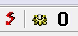
\includegraphics[scale=0.7]{figuras/restartIFR-HDR.png} .
            \end{itemize}
        \end{minipage}
        \Extradetail
    }
}
% #endregion

% #region       MeasureRfDataCharacteristicsOnCortexWithBer{folder}
\newcommand{\MeasureRfDataCharacteristicsOnCortexWithBer}[1]
{
    \stepcounter{Step}
    \procedurestep{\theSec}{\theStep}{EXE}{Measure Data characteristics in DMU-#1 and DPU-#1 of \textbf{\cortexHDR{}} of \gse{}}{
\textbf{Eb/N0:}\_\_\_\_\_\_\\
\textbf{IF Level:}\_\_\_\_\_\_\\
\textbf{EVM:}\_\_\_\_\_\_\\
\textbf{Ampli Err:}\_\_\_\_\_\_\\
\textbf{Phase Err:}\_\_\_\_\_\_\\
\textbf{BER:}\_\_\_\_\_\_\\
\textbf{Nb. error:}\_\_\_\_\_\_\\
}{\Result}{\Status}
    \stepdetail{1}{0}{
        Go to MCS Cortex (\hdrIP{}) of \fmr{} do the following:
        \begin{minipage}[t]{\linewidth}
            \begin{itemize}[nosep,after=\strut]
                \item In Vector tab of DMU-#1, read the following parameters: \textbf{Eb/N0},\textbf{IF Level},\textbf{EVM}, \textbf{Ampli Err} and \textbf{Phase Err.}
                \item In the BER-FER tab of DPU-#1, read the following parameters: \textbf{BER} and \textbf{Number of error}.
            \end{itemize}
        \end{minipage}
    }
}
% #endregion

% #region       TakeScreenShotInCortexHdrGse
\newcommand{\TakeScreenShotInCortexHdrGse}[2]
{
    \stepcounter{Step}
    \immediate\write\myfile{|\theSec|\theStep|TakeScreenShotInCortexHdrGse|}
    \procedurestep{\theSec}{\theStep}{EXE}{Take screenshot of signal measurement.}{\texttt{#2} saved.}{}{}
    \stepdetail{1}{0}{
        Save screenshot of MCS (\hdrIP{}) in #1 folder with name #2. This could be done by pressing the \textbf{print screen key} and using 
        the Paint software.
    }

}
% #endregion

% #region       MeasureRfDataCharacteristicsOnCortex{folder}
\newcommand{\MeasureRfDataCharacteristicsOnCortex}
{
    \stepcounter{Step}
    \procedurestep{\theSec}{\theStep}{EXE}{Measure Data characteristics in \textbf{\cortexHDR{}} of \gse{}}{
\textbf{Eb/N0:}\_\_\_\_\_\_\\
\textbf{IF Level:}\_\_\_\_\_\_\\
\textbf{EVM:}\_\_\_\_\_\_\\
\textbf{Ampli Err:}\_\_\_\_\_\_\\
\textbf{Phase Err:}\_\_\_\_\_\_\\
}{\Result}{\Status}
    \stepdetail{1}{0}{
        Go to MCS Cortex (\hdrIP{}) of \fmr{}, in Vector tab, do the following:
        \begin{minipage}[t]{\linewidth}
            \begin{itemize}[nosep,after=\strut]
                \item Press reset button and wait 20 seconds.
                \item Read the following parameters: \textbf{Eb/N0},\textbf{IF Level},\textbf{EVM}, \textbf{Ampli Err} and \textbf{Phase Err.}
            \end{itemize}
        \end{minipage}
    }
}
% #endregion
% #region       CompleteReportTable{table name}
% \newcommand{\CompleteReportTable}
% {
%     \stepcounter{Step}
%     \immediate\write\myfile{|\theSec|\theStep|CompleteReportTable|}
%     \procedurestep{\theSec}{\theStep}{EXE}{Complete the reporting  table.}{Table filled.}{\Result}{\Status}
%     \stepdetail{1}{0}{Complete the reporting table \ref{tab:tm-filter}.\\
    
%         \Extradetail
%     }
% }
% #endregion

% #region       RegisterBestDataFilterBasic
\newcommand{\RegisterBestDataFilterBasic}
{
    \stepcounter{Step}
    \immediate\write\myfile{|\theSec|\theStep|RegisterBestDataFilterBasic|}
    \procedurestep{\theSec}{\theStep}{EXE}{
Take note of the best filter parameters for Data demodulation.
}{
Option config \#: x
}{\Result}{\Status}
    \stepdetail{1}{0}{
    Take note of the best filter parameters acording to:\\
    Highest Eb/N0 value, the minimum EVM value, the minimum Amplitude error and minimum Phase error.\\\Extradetail
    }
}
% #endregion





% #region       configureAdvancedParametersOnCortexHdrGse{filter}{alpha}
\newcommand{\configureAdvancedParametersOnCortexHdrGse}[1]
{

    \stepcounter{Step}
    \procedurestep{\theSec}{\theStep}{EXE}{Configure the matched filter on Cortex HDR of \gse{}.}{Cortex HDR configured.}{\Result}{\Status}
    \stepdetail{1}{0}{
        Go to MCS Cortex (\hdrIP{}) of \gse{}:
        \begin{minipage}[t]{\linewidth}
            \begin{itemize}[nosep,after=\strut]
                \item In the Global tab of DMU-1 (Demodulator Unit 1) do the following:
                      \begin{itemize}[nosep,after=\strut]
                        \item click the \textbf{Config} button.
                        \ifstrequal{#1}{B2}{
                            \item Set Asym = \textbf{ON} 
                            \item Set Comp = \textbf{ON} 
                            \item Set LMS = OFF
                            \item Set 4*Sr = OFF
                            \item Set DEAF = OFF
                            \item Set CMA  = \textbf{ON}
                            \item Set Fast = OFF
                            \item Set XDEAF = OFF
                            \item Set LPF = \textbf{ON}
                            \item Set HBF = \textbf{ON}}{}
                        \ifstrequal{#1}{1}{
                          \item Set Asym = OFF 
                          \item Set Comp = OFF 
                          \item Set LMS = \textbf{ON}
                          \item Set 4*Sr = OFF
                          \item Set DEAF = OFF
                          \item Set CMA  = OFF
                          \item Set Fast = OFF
                          \item Set XDEAF = OFF
                          \item Set LPF = OFF
                          \item Set HBF = OFF}{}
                        \ifstrequal{#1}{2}{
                          \item Set Asym = OFF 
                          \item Set Comp = OFF 
                          \item Set LMS = OFF
                          \item Set 4*Sr = OFF
                          \item Set DEAF = OFF
                          \item Set CMA  = \textbf{ON}
                          \item Set Fast = OFF
                          \item Set XDEAF = OFF
                          \item Set LPF = OFF
                          \item Set HBF = OFF}{}
                        \ifstrequal{#1}{3}{
                          \item Set Asym = \textbf{ON} 
                          \item Set Comp = \textbf{ON} 
                          \item Set LMS = \textbf{ON}
                          \item Set 4*Sr = OFF
                          \item Set DEAF = OFF
                          \item Set CMA  = OFF
                          \item Set Fast = OFF
                          \item Set XDEAF = OFF
                          \item Set LPF = OFF
                          \item Set HBF = OFF}{}
                        \ifstrequal{#1}{4}{
                          \item Set Asym = \textbf{ON} 
                          \item Set Comp = \textbf{ON} 
                          \item Set LMS = \textbf{ON}
                          \item Set 4*Sr = \textbf{ON}
                          \item Set DEAF = OFF
                          \item Set CMA  = OFF
                          \item Set Fast = OFF
                          \item Set XDEAF = OFF
                          \item Set LPF = OFF
                          \item Set HBF = OFF}{}
                        \ifstrequal{#1}{5}{
                          \item Set Asym = \textbf{ON} 
                          \item Set Comp = \textbf{ON} 
                          \item Set LMS = \textbf{ON}
                          \item Set 4*Sr = OFF
                          \item Set DEAF = OFF
                          \item Set CMA  = OFF
                          \item Set Fast = OFF
                          \item Set XDEAF = OFF
                          \item Set LPF = \textbf{ON}
                          \item Set HBF = \textbf{ON}}{}
                        \ifstrequal{#1}{6}{
                          \item Set Asym = OFF 
                          \item Set Comp = OFF 
                          \item Set LMS = \textbf{ON}
                          \item Set 4*Sr = OFF
                          \item Set DEAF = \textbf{ON}
                          \item Set CMA  = OFF
                          \item Set Fast = OFF
                          \item Set XDEAF = OFF
                          \item Set LPF = OFF
                          \item Set HBF = OFF}{}
                        \ifstrequal{#1}{7}{
                          \item Set Asym = OFF 
                          \item Set Comp = OFF 
                          \item Set LMS = OFF
                          \item Set 4*Sr = OFF
                          \item Set DEAF = \textbf{ON}
                          \item Set CMA  = \textbf{ON}
                          \item Set Fast = OFF
                          \item Set XDEAF = OFF
                          \item Set LPF = OFF
                          \item Set HBF = OFF}{}
                        \ifstrequal{#1}{8}{
                          \item Set Asym = \textbf{ON} 
                          \item Set Comp = \textbf{ON} 
                          \item Set LMS = \textbf{ON}
                          \item Set 4*Sr = OFF
                          \item Set DEAF = \textbf{ON}
                          \item Set CMA  = OFF
                          \item Set Fast = OFF
                          \item Set XDEAF = OFF
                          \item Set LPF = OFF
                          \item Set HBF = OFF}{}
                        \ifstrequal{#1}{9}{
                          \item Set Asym = \textbf{ON} 
                          \item Set Comp = \textbf{ON} 
                          \item Set LMS = OFF
                          \item Set 4*Sr = OFF
                          \item Set DEAF = \textbf{ON}
                          \item Set CMA  = \textbf{ON}
                          \item Set Fast = OFF
                          \item Set XDEAF = OFF
                          \item Set LPF = OFF
                          \item Set HBF = OFF}{}
                        \ifstrequal{#1}{10}{
                          \item Set Asym = \textbf{ON} 
                          \item Set Comp = \textbf{ON} 
                          \item Set LMS = \textbf{ON}
                          \item Set 4*Sr = OFF
                          \item Set DEAF = \textbf{ON}
                          \item Set CMA  = OFF
                          \item Set Fast = OFF
                          \item Set XDEAF = OFF
                          \item Set LPF = \textbf{ON}
                          \item Set HBF = \textbf{ON}}{}
                        \ifstrequal{#1}{11}{
                          \item Set Asym = \textbf{ON} 
                          \item Set Comp = \textbf{ON} 
                          \item Set LMS = \textbf{ON}
                          \item Set 4*Sr = OFF
                          \item Set DEAF = \textbf{ON}
                          \item Set CMA  = OFF
                          \item Set Fast = \textbf{ON}
                          \item Set XDEAF = OFF
                          \item Set LPF = \textbf{ON}
                          \item Set HBF = \textbf{ON}}{}
                        \ifstrequal{#1}{12}{
                          \item Set Asym = \textbf{ON} 
                          \item Set Comp = \textbf{ON} 
                          \item Set LMS = OFF
                          \item Set 4*Sr = OFF
                          \item Set DEAF = \textbf{ON}
                          \item Set CMA  = \textbf{ON}
                          \item Set Fast = OFF
                          \item Set XDEAF = OFF
                          \item Set LPF = \textbf{ON}
                          \item Set HBF = \textbf{ON}}{}
                        \ifstrequal{#1}{13}{
                          \item Set Asym = \textbf{ON} 
                          \item Set Comp = \textbf{ON} 
                          \item Set LMS = ON
                          \item Set 4*Sr = OFF
                          \item Set DEAF = \textbf{ON}
                          \item Set CMA  = \textbf{ON}
                          \item Set Fast = \textbf{ON}
                          \item Set XDEAF = OFF
                          \item Set LPF = \textbf{ON}
                          \item Set HBF = \textbf{ON}}{}
                          \item click the \textbf{Apply} button.
                      \end{itemize}
            \end{itemize}
        \end{minipage}
        \Extradetail
    }
}
% #endregion

%#region       CopyCortexHdrScreenShotsToCegseForEvidences
\newcommand{\CopyCortexHdrScreenShotsToCegseForEvidences}[1]
{
    \stepcounter{Step}
    \immediate\write\myfile{|\theSec|\theStep|CopyCortexHdrScreenShotsToCegseForEvidences|}
    \procedurestep{\theSec}{\theStep}{EXE}{Copy screenshots folder of Cortex HDR to \comEgse{}.}{Folder copied}{}{}
    \stepdetail{1}{0}{In the \comEgse{}:
        \begin{minipage}[t]{\linewidth}
            \begin{itemize}[nosep,after=\strut]
                \item Open the file explorer and connect to Cortex HDR (\hdrIP{}) with the following credentials:
                      \begin{itemize}[nosep,after=\strut]
                          \item Address: \bs{}\bs{}\hdrIP{}
                          \item {User: cortex}
                          \item {Password: cortex}
                      \end{itemize}
                \item Go to \bs{}\bs{}\hdrIP{}\bs{}zds\bs{}HDR\bs{}MCS\bs{}
                \item Copy the screenshots folder #1.
                \item Go to \texttt{\comEgseTestFolderLocation{}\comEgseTestFolderName{}\bs{}\\
                \sessionID{}\bs{}\procid{}\bs{}\subprocid{}} directory of \comEgse{}.
                \item Paste the copied folder.
                \item Go to \bs{}\bs{}\hdrIP{}\bs{}zds\bs{}HDR\bs{}MCS\bs{}
                \item Delete the folder #1 from Cortex HDR.
            \end{itemize}
        \end{minipage}
    }
}



% #region       CloseCortexConfigFileHdrGse
\newcommand{\CloseCortexConfigFileHdrGse}
{
    \stepcounter{Step}
    \immediate\write\myfile{|\theSec|\theStep|CloseCortexConfigFileHdrGse|}
    \procedurestep{\theSec}{\theStep}{EXE}{Close \textbf{Cortex HDR of \gse{}} configuration file.}{File closed.}{\Result}{\Status}
    \stepdetail{1}{0}{In Cortex MCS close configuration file \textbf{without save changes}. Go to \textbf{File>Close} and then click \textbf{No}.\\~\\
        %Note: If the next RF test is carried out, skip this step.
        \Extradetail
    }
}
% #endregion

%%%%%%%%%%%%%%%%%%%%%%%%%%%%%%%%%%%%%%%%%%%%%%%%%%%%%%%%%%%%%%%%%%%%%%%%%%%%%%%%%%%%%%%%%%%%%%%%%%%%%%%
%%%% Vector script
%%%%%%%%%%%%%%%%%%%%%%%%%%%%%%%%%%%%%%%%%%%%%%%%%%%%%%%%%%%%%%%%%%%%%%%%%%%%%%%%%%%%%%%%%%%%%%%%%%%%%%

\newcommand{\VectorStar}{
\SimpleExeStep{Start Vector script}{Vector script started\\ YYYYMMDDHHMMSS: }
{
   In the terminal window of \vmTesting (\vmTestingIP) run the following commands:
   \begin{itemize}[noitemsep]
       \item \texttt{cd /verification/Vector}
       \item \texttt{date} 
       \item \texttt{sh vector.sh}
   \end{itemize}
   Then take note of date.
}
}
\newcommand{\VectorVerify}{
\SimpleExeStep{Verify connection of clients in \cortexHDR}
{Clients conected a \cortexHDR}
{According to the figure below, do the following:
\begin{itemize}[noitemsep]
   \item Go to MCS Cortex (192.168.75.161), in the Global window
   \begin{itemize}
       \item Verify client connection 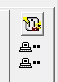
\includegraphics[scale=0.7]{figuras/clientHDR.png}
    \end{itemize}
\end{itemize} 
}
}
\newcommand{\VectorStop}{
\SimpleExeStep{Stop Vector script}{Vector script stoped}
{
   \begin{itemize}[noitemsep]
       \item Wait 30 seconds 
       \item Go to terminal were Vector script was executed and press Ctrl + C
   \end{itemize} 	
}
}
\newcommand{\VectorGetEVM}[1]
{
\SimpleExeStep{Get EVM value}
{ EVM [\%] value}
{
    From the file explorer in the \vmTesting (\vmTestingIP)
\begin{itemize}
    \item Go to the \texttt{/opt/sao/appsharedfiles/Vector/workspace} directory
    \item Open \texttt{Vector-HDR\_DMU1\_Vector-100<YYYYMMDDHHMMSS>-<YYYYMMDDTHHMMSS>-001.scv }
    file created later than the date taken in vector script start step for \textbf{#1}.
    \item Get average value of \textbf{DMU.EVM.Calc.Normalized.percent}.
\end{itemize}

}
}

% #region       CopyFilesToMgmtFromDatasetOnPxi
\newcommand{\CopyFilesToCEGEFromMgmt}[1]
{
\SimpleExeStep{Copy files to \comEgse from \vmTesting.}
{files copied.}
{  On EGSE open Total Commander from shocut in desktop and do de following:
\begin{itemize}
    \item On left side go to C:/Users/EGSE COM/Documents/COMM-SS-FM/\sessionID/\procid/\subprocid/
    \item On rigth side go "Network Neighborhood", select [Secure FTP], press F7 and connect to GS-GSE.MGMT VM with the following paremeters:
          \begin{itemize}
              \item 192.168.75.193
              \item User: administrator
              \item Password: Sb1.C0n43
          \end{itemize}
    \item On rigth side go to /opt/sao/appsharedfiles/Vector/output/ directory.
    \item Find and copy \texttt{Vector-HDR-100<YYYYMMDDHHMMSS>-<YYYYMMDDTHHMMSS>.tar.gz} files
    created after the date taken in the step where the Vector script for \textbf{#1} was started.
    \item Page files .tar.gz in C:/Users/EGSE COM/Documents/COMM-SS-FM/\sessionID/\procid/\subprocid/
\end{itemize}}

   
}
% #endregion

% #region       ConfigureCortexHdrForBERMeasurementOnChannel{\modemCfgRFBB}{Note}
\newcommand{\ConfigureCortexHdrForBERMeasurementOnChannel}[1]
{
    \stepcounter{Step}
    \immediate\write\myfile{|\theSec|\theStep|ConfigureCortexHdrForBERMeasurementOnChannel|}
    \procedurestep{\theSec}{\theStep}{EXE}{Configure Cortex HDR for BER measurement }{Cortex HDR configured for BER measurement.}{\Result}{\Status}
    \stepdetail{1}{0}{
        Go to MCS Cortex (192.168.75.161) and do the following:
        \begin{minipage}[t]{\linewidth}
            \begin{itemize}[nosep,after=\strut]
                \item In the Global window, click on the DMU-#1(Demodulator Unit #1).
                \begin{itemize}
                    \item In the displayed window go to BER tab. 
                    \item Click on Config button.
                    \item In Operating Mode select : File.
                    \item In File Number DPU1: 52050
                    \item Click on Apply button.
                \end{itemize}
                \item In the Global window, click on the DPU-#1(Data Procesor Unit #1)
                 \begin{itemize}
                    \item In the displayed window go to BER-FER tab. 
                    \item Click on Config button.
                    \item In Operating Mode select : File.
                    \item In File Number: 52050
                    \item Click on Apply button.
                \end{itemize}
            \end{itemize}
        \end{minipage} \\~\\\Extradetail
    }
}
% #endregion
% #region       OpenMcsWindowsInCortexHdrGseForOneChannelTest{Folder Name}
\newcommand{\OpenMcsWindowsInCortexHdrGseForOneChannelTest}
{
    \stepcounter{Step}
    \procedurestep{\theSec}{\theStep}{EXE}{Open Global,BER, Spectrum, Vector and Recording Global tabs in Cortex HDR of GS-GSE-FM (R).}{tabs open.}{}{}
    \stepdetail{1}{0}{
Go to MCS Cortex (192.168.75.161). According to the figures below, do the following:
        \begin{minipage}[t]{\linewidth}
            \begin{itemize}[nosep,after=\strut]
                \item Global tab of DMU-1 (Demodulator Unit 1):
                \begin{itemize}
                    \item In the Global window, click on the DMU-1.
                    \item In the displayed window go to Global tab.
                \end{itemize}
                \item BER tab of DMU-1:
                \begin{itemize}
                    \item In the Global window, click on the DMU-1.
                    \item In the displayed window go to BER tab.
                \end{itemize}
                \item Spectrum tab of DMU-1:
                \begin{itemize}
                    \item In the Global window, click on the DMU-1.
                    \item In the displayed window go to Spectrum tab and press enable button.
                \end{itemize}
                \item Vector tab of DMU-1:
                \begin{itemize}
                    \item In the Global window, click on the DMU-1.
                    \item In the displayed window go to vector tab, select cumulative option and press enable button.
                \end{itemize}
                \item BER-FER tab of DPU-1:
                \begin{itemize}
                    \item In the Global window, click on the DPU-1 (Data Procesor Unit 1).
                    \item In the displayed window go to BER-FER tab.
                \end{itemize}
                \item Global tab of DRU-1:
                \begin{itemize}
                    \item In the Global window, click on the DRU-1 (Data Recording Unit 1).
                    \item In the displayed window go to Recording Global tab.
                \end{itemize}
            \end{itemize}
        \end{minipage}
        \begin{center}
            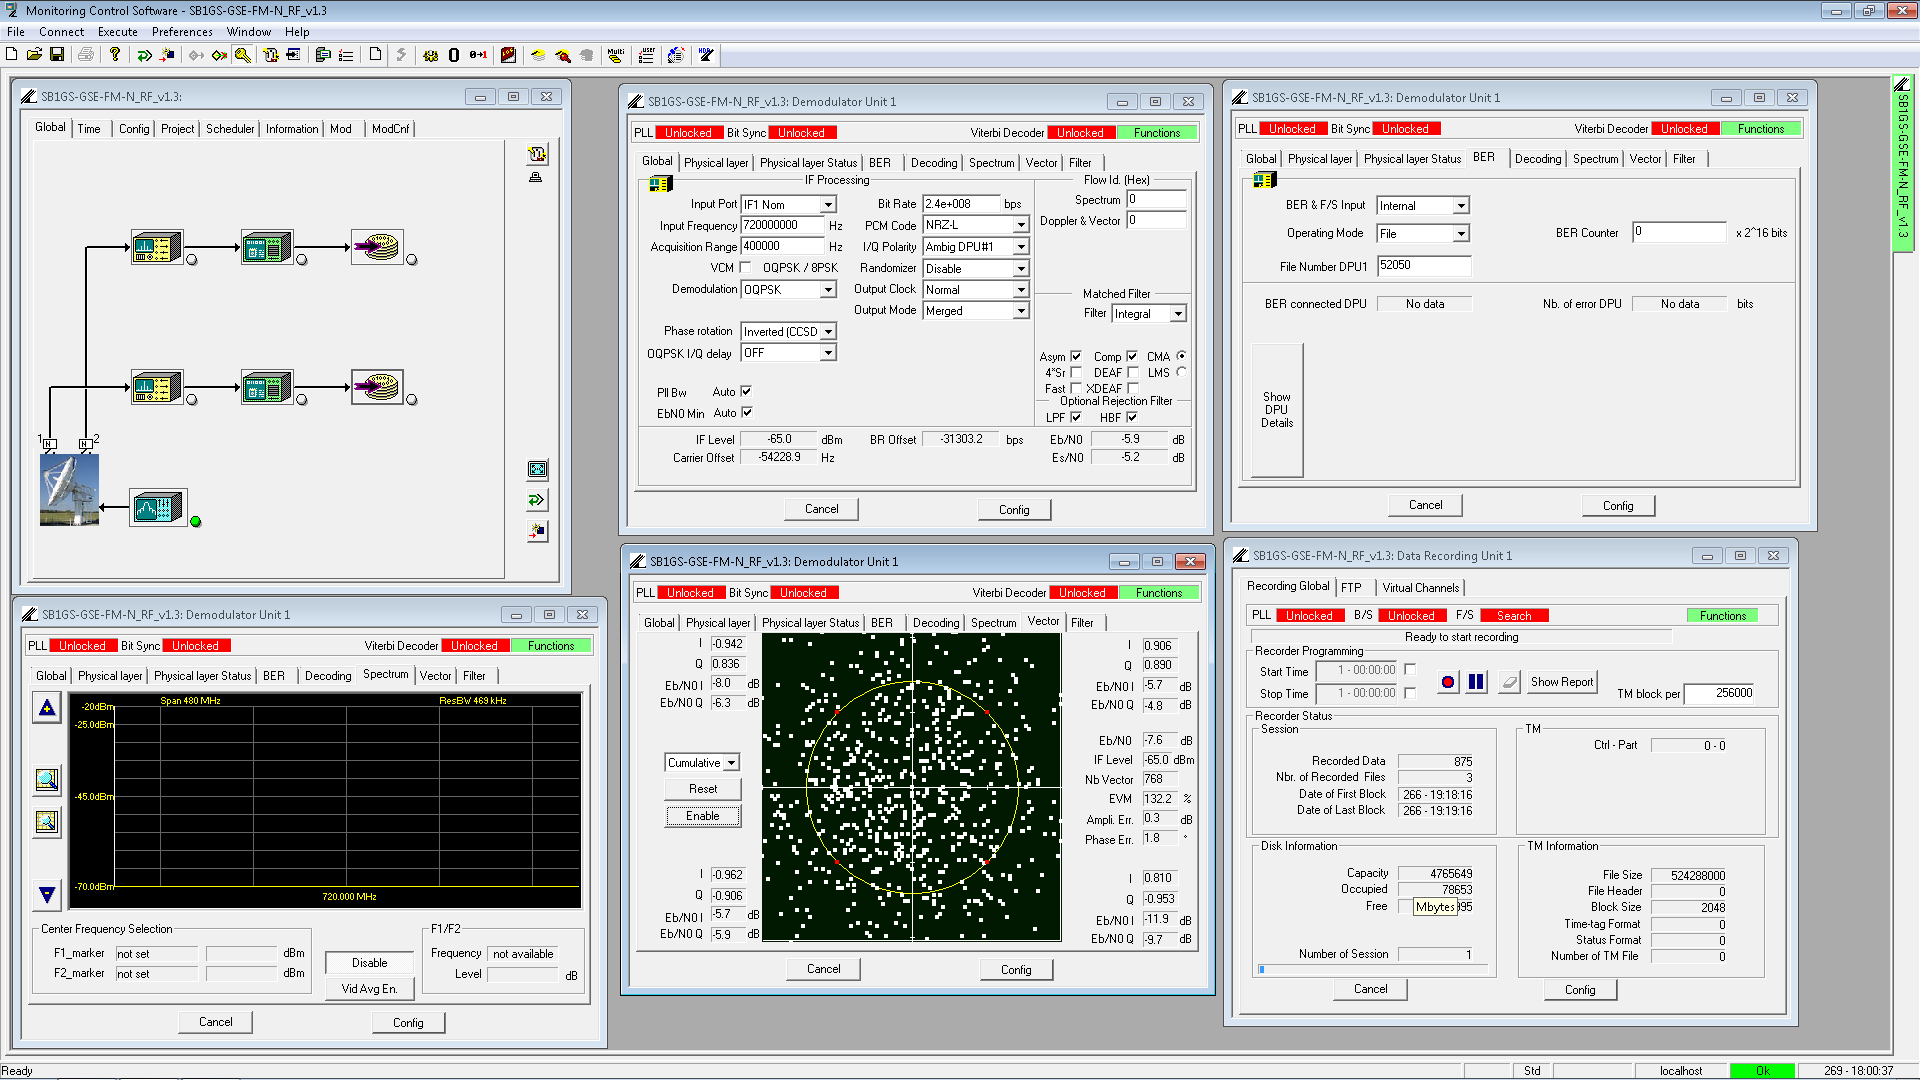
\includegraphics[width=0.53\textwidth]{figuras/cortex-hdr-one-channel.png}
        \end{center}              
    }
}


%%%%%%%%%%%%%%%%%%%%%%%%%%%%%%%%%%%%%%%%%%%%%%%%%%%%%%%%%%%%%%%%%%%%%%%%%%%%
% #region       ConfigureXBandUpConverterNOneRfTestBed{Att}{Output}{script}
% \newcommand{\ConfigureXBandUpConverterNOneRfTestBed}[3]
% {
%     \stepcounter{Step}
%     \procedurestep{\theSec}{\theStep}{EXE}{
%  Configure X-Band Upconverter of RF TestBed.
% }{
% Freq = 8269.0 MHz\\
% Aten = #1\\
% RF = #2
% }{}{}
%     \stepdetail{1}{0}{
%     In the terminal window of GS-GSE.MGMT VM (192.168.75.193) of \fmr{} run the following commands:
%         \begin{minipage}[t]{\linewidth}
%             \begin{itemize}[nosep,after=\strut]
%                 \item cd /verification/COMM-SS-FM/session\_ID/
%                 \item python #3
%             \end{itemize}
%         \end{minipage}   
% In the displayed menu, verify that parameter configured are according  to the expected values.
%     }
% }



\newcommand{\ConfigureXBandUpConverterNOneRfTestBed}[3]
{
    \stepcounter{Step}
    \immediate\write\myfile{|\theSec|\theStep|ConfigureXBandUpConverterNOneRfTestBed|}
    \procedurestep{\theSec}{\theStep}{EXE}{ Configure X-Band Upconverter of RF TestBed.}{
        \begin{minipage}[t]{\linewidth}
            \begin{itemize}[nosep,after=\strut,leftmargin=*]
                \item RF = 8106.0 MHz for \textbf{EWC30-FM2}
                \item RF = 8269.0 MHz for \textbf{EWC30-FM1}

                \item Aten = #1
                \item RF = #2
            \end{itemize}
        \end{minipage}
    }{\Result}{\Status}
    \stepdetail{1}{0}{

        In the terminal window of \vmTesting{} (\vmTestingIP{}) of \fmr{} run the following commands:
        \begin{minipage}[t]{\linewidth}
            \begin{itemize}[nosep,after=\strut]
                \item \texttt{cd /verification/COMM-SS-FM/session\_ID/ }
                \item \texttt{python #3}
            \end{itemize}
        \end{minipage}
        In the displayed menu, do the following:
        \begin{minipage}[t]{\linewidth}
            \begin{itemize}[nosep,after=\strut]
                \item Configure Aten = #1.
                \item Configure Freq = 8269 MHz for \textbf{EWC30-FM1} and 8106 for \textbf{EWC30-FM2}.
                \item Verify that RF = #2
            \end{itemize}
        \end{minipage}
      %  Then enter the number 5 and press enter to exit the menu.\\
        \Extradetail
    }
}






% #region       ConfigureXBandDownConverterNOneRfTestBed{Att}{Output}{script}
\newcommand{\ConfigureXBandDownConverterNOneRfTestBed}[3]
{
    \stepcounter{Step}
    \procedurestep{\theSec}{\theStep}{EXE}{
 Configure X-Band Downconverter of RF TestBed.
}{
Freq = 8106.0 MHz\\
Aten = #1\\
RF = #2
}{}{}
    \stepdetail{1}{0}{
From GS-GSE-FM (N) In the terminal window of GS-GSE.MGMT VM (192.168.75.193) run the following commands:
        \begin{minipage}[t]{\linewidth}
            \begin{itemize}[nosep,after=\strut]
                \item cd /verification/COMM-SS-EM-PT/session\_ID/
                \item python #3
            \end{itemize}
        \end{minipage}   
In the displayed menu, verify that parameter configured are according  to the expected values.
    }
}

% #region       ConfigureCortexHdrRfTestBed
\newcommand{\ConfigureCortexHdrRfTestBed}[1]
{
    \stepcounter{Step}
    \immediate\write\myfile{|\theSec|\theStep|ConfigureCortexHdrGse|}
    \procedurestep{\theSec}{\theStep}{EXE}{
Configure the \textbf{\cortexHDR{}} of TestBed.
}{
\cortexHDR{} configured.
}{\Result}{\Status}
    \stepdetail{1}{0}{In Cortex MCS (\hdrTBIP{}) open the configuration file #1 from directory \hdrTBCfgFileDir{}\texttt, enable configuration by clicking on the \textbf{Control Access} icon (key icon) and click the \textbf{OK} button. Then click on \textbf{Copy Cnf->Mon} icon and then click yes if needed.
    \Extradetail
    }
}
% #endregion


% #region       EnableNOneAndNTwoInterfaceXBand
\newcommand{\EnableNOneAndNTwoInterfaceXBand}
{
    \stepcounter{Step}
    \immediate\write\myfile{|\theSec|\theStep|EnableNOneInterfaceXBand|}
    \procedurestep{\theSec}{\theStep}{EXE}{Enable \textbf{N1} and \textbf{N2} interfaces in the \textbf{\XBMA{}}.}{N1 and N2 interfaces enabled.}{\Result}{\Status}
    \stepdetail{1}{0}{

        In the \xbmaSof{} software run on \vmWin{} (\vmWinIP{}):
        \begin{minipage}[t]{\linewidth}
            \begin{itemize}[nosep,after=\strut]
                \item Go to the \textbf{Nadir 1 Transfer Switch Control} field and press the \textbf{Nadir 1 to Down Converters} button.
                \item Go to the \textbf{XBMA Control Diagram} field and verify that the bottom indicator of the \textbf{N1 TRANSFER SWITCH} block is \textbf{ON} and green.
                \item Go to the \textbf{Nadir 2 Transfer Switch Control} field and press the \textbf{Nadir 2 to Down Converters} button.
                \item Go to the \textbf{XBMA Control Diagram} field and verify that the upper indicator of the \textbf{N2 TRANSFER SWITCH} block is \textbf{ON} and green.
            \end{itemize}
        \end{minipage}
    }
}
% #endregion


% #region       EnableNoiseGenerationInCortexHdrTestBed
\newcommand{\EnableNoiseGenerationInCortexHdrTestBed}
{
    \stepcounter{Step}
    \immediate\write\myfile{|\theSec|\theStep|EnableNoiseGenerationInCortexHdrTestBed|}
    \procedurestep{\theSec}{\theStep}{EXE}{Enable noise generation in \textbf{\cortexHDR{} of \tbed{}}.}{Noise Enabled.}{}{}
    \stepdetail{1}{0}{
        Go to MCS Cortex (\hdrTBIP{}) and in Global window of TMU (Test Modulator Unit) do the folowing:
        \begin{minipage}[t]{\linewidth}
            \begin{itemize}[nosep,after=\strut]
                \item Click on \textbf{Config} button.
                \item Mark \textbf{Noise Enable} field.
                \item Click on \textbf{Apply} button.
            \end{itemize}
        \end{minipage}
    }
}
% #endregion

% #region       DisableNoiseGenerationInCortexHdrTestBed
\newcommand{\DisableNoiseGenerationInCortexHdrTestBed}
{
    \stepcounter{Step}
    \immediate\write\myfile{|\theSec|\theStep|DisableNoiseGenerationInCortexHdrTestBed|}
    \procedurestep{\theSec}{\theStep}{EXE}{Disable noise generation in \textbf{\cortexHDR{} of \tbed{}}.}{Noise disabled.}{}{}
    \stepdetail{1}{0}{
        Go to MCS Cortex (\hdrTBIP{}) and in Global window of TMU (Test Modulator Unit) do the folowing:
        \begin{minipage}[t]{\linewidth}
            \begin{itemize}[nosep,after=\strut]
                \item Click on \textbf{Config} button.
                \item UnMark \textbf{Noise Enable} field.
                \item Click on \textbf{Apply} button.
            \end{itemize}
        \end{minipage}
    }
}
% #endregion

% #region       OpenMcsWindowsCortexHdrTestBed
\newcommand{\OpenMcsWindowsCortexHdrTestBed}
{
    % Step - Crear carpeta de capturas en cortex
    \stepcounter{Step}
    \procedurestep{\theSec}{\theStep}{EXE}{Open TMU window in Cortex HDR of GS-GSE-FM (R).}{Windows open.}{}{}
    \stepdetail{1}{0}{
Go to MCS Cortex (\hdrTBIP{})and do the following:
        \begin{minipage}[t]{\linewidth}
            \begin{itemize}[nosep,after=\strut]
                \item In the Global window, click on the TMU-1(Test Modulator Unit).
            \end{itemize}
        \end{minipage}                
    }
}


% #region       ConnectRfCableToXBandTestPortOf
\newcommand{\ConnectCableToRfOutputOfCortexHdrTestBed}[1]
{
    \stepcounter{Step}
    \immediate\write\myfile{|\theSec|\theStep|ConnectRfCableToXBandTestPortOf,CABLE=#1|}
    \procedurestep{\theSec}{\theStep}{EXE}{Connect \textbf{#1} cable to IF output of Cortex HDR of TestBed}{Cable #1 connected IF output of Cortex HDR}{\Result}{\Status}
    \stepdetail{1}{0}{
        \begin{minipage}[t]{\linewidth}
            \begin{itemize}[nosep,after=\strut]
                \item Connect #1 cable to IF output of Cortex HDR (J50 IF out).
            \end{itemize}
        \end{minipage}
    }
}
% #endregion

% #region       ConnectCableToIfOutputOfDownConverterTestBed
\newcommand{\ConnectCableToIfOutputOfDownConverterTestBed}[1]
{
    \stepcounter{Step}
    \immediate\write\myfile{|\theSec|\theStep|ConnectCableToIfOutputOfDownConverterTestBed,CABLE=#1|}
    \procedurestep{\theSec}{\theStep}{EXE}{Connect \textbf{#1} cable to IF output of X-Band Downconverter of TestBed}{Cable #1 connected IF output of X-Band Downconverter of RF TestBed}{\Result}{\Status}
    \stepdetail{1}{0}{
        \begin{minipage}[t]{\linewidth}
            \begin{itemize}[nosep,after=\strut]
                \item Connect the free end of \textbf{#1} cable to IF output of X-Band Downconverter of TestBed.
            \end{itemize}
        \end{minipage}
    }
}
% #endregion

% #region       DisconnectCableFromRfOutputOfCortexHdrTestBed
\newcommand{\DisconnectCableFromRfOutputOfCortexHdrTestBed}[2]
{
    \stepcounter{Step}
    \immediate\write\myfile{|\theSec|\theStep|DisconnectCableFromRfOutputOfCortexHdrTestBed,CABLE=#1|}
    \procedurestep{\theSec}{\theStep}{EXE}{Disconnect \textbf{#1} cable from IF output of Cortex HDR of TestBed}{Cable #1 disconnected from IF output of Cortex HDR}{\Result}{\Status}
    \stepdetail{1}{0}{
        \begin{minipage}[t]{\linewidth}
            \begin{itemize}[nosep,after=\strut]
                \item Disconnect #1 cable from IF output of Cortex HDR (J50 IF out).
            \end{itemize}
        \end{minipage}\\#2
    }
}
% #endregion


% #region       DisconnectCableFromIfOutputOfDownconverterTestBed
\newcommand{\DisconnectCableFromIfOutputOfDownconverterTestBed}[2]
{
    \stepcounter{Step}
    \immediate\write\myfile{|\theSec|\theStep|DisconnectCableFromIfOutputOfDownconverterTestBed,CABLE=#1|}
    \procedurestep{\theSec}{\theStep}{EXE}{Disconnect \textbf{#1} cable from IF output of X-Band Downconverter of TestBed}{Cable #1 disconnected from IF output of X-band Downconverter}{\Result}{\Status}
    \stepdetail{1}{0}{
        \begin{minipage}[t]{\linewidth}
            \begin{itemize}[nosep,after=\strut]
                \item Disconnect #1 cable from IF output of X-Band Downconverter of RF TestBed.
            \end{itemize}
        \end{minipage}\\#2
    }
}
% #endregion


% #region       ConnectCableToRFOutputOfUpconverterTestBed
\newcommand{\ConnectCableToRFOutputOfUpconverterTestBed}[1]
{
    \stepcounter{Step}
    \immediate\write\myfile{|\theSec|\theStep|ConnectCableToRFOutputOfUpconverterTestBed,CABLE=#1|}
    \procedurestep{\theSec}{\theStep}{EXE}{Connect \textbf{#1} cable to RF output (J2) of Upconverter of TestBed}{Cable #1 connected RF output of Upconverter}{\Result}{\Status}
    \stepdetail{1}{0}{
        \begin{minipage}[t]{\linewidth}
            \begin{itemize}[nosep,after=\strut]
                \item Connect #1 cable to RF output of Upconverter.
            \end{itemize}
        \end{minipage}
    }
}
% #endregion


% #region       DisconnectCableFromRFOutputOfUpconverterTestBed
\newcommand{\DisconnectCableFromRFOutputOfUpconverterTestBed}[2]
{
    \stepcounter{Step}
    \immediate\write\myfile{|\theSec|\theStep|DisconnectCableFromRFOutputOfUpconverterTestBed,CABLE=#1|}
    \procedurestep{\theSec}{\theStep}{EXE}{Disconnect \textbf{#1} cable from RF output of Upconverter of TestBed}{Cable #1 disconnected from RF output of Upconverter}{\Result}{\Status}
    \stepdetail{1}{0}{
        \begin{minipage}[t]{\linewidth}
            \begin{itemize}[nosep,after=\strut]
                \item Disconnect #1 cable from RF output of Upconverter.
            \end{itemize}
        \end{minipage}\\#2
    }
}
% #endregion


% #region       EnableRfOutputXbandUpconverterTestBed
\newcommand{\EnableRfOutputXbandUpconverterTestBed}
{
    \stepcounter{Step}
    \immediate\write\myfile{|\theSec|\theStep|EnableRfOutputXbandUpconverterTestBed|}
    \procedurestep{\theSec}{\theStep}{EXE}{
Enable RF output of X-Band Upconverter of \tbed{}
}{
RF output ON.
}{}{}
    \stepdetail{1}{0}{
 Go to the X-Band Upconverter  configuration menu in the terminal window and do the following:
        \begin{minipage}[t]{\linewidth}
            \begin{itemize}[nosep,after=\strut]
                \item Press the 3 key and then enter.
                \item Press the 1 key and then enter
                \item Click on \textbf{Apply} button.
            \end{itemize}
        \end{minipage}
        Verify that the desired parameter was configured correctly by viewing the menu display.
    }
}
% #endregion

% #region       EnableRfOutputXbandDownconverterTestBed
\newcommand{\EnableRfOutputXbandDownconverterTestBed}
{
    \stepcounter{Step}
    \immediate\write\myfile{|\theSec|\theStep|EnableRfOutputXbandDownconverterTestBed|}
    \procedurestep{\theSec}{\theStep}{EXE}{
Enable RF output of X-Band Downconverter of \tbed{}
}{
RF output ON.
}{}{}
    \stepdetail{1}{0}{
 Go to the X-Band Downconverter  configuration menu in the terminal window and do the following:
        \begin{minipage}[t]{\linewidth}
            \begin{itemize}[nosep,after=\strut]
                \item Press the 3 key and then enter.
                \item Press the 1 key and then enter
                \item Click on \textbf{Apply} button.
            \end{itemize}
        \end{minipage}
        Verify that the desired parameter was configured correctly by viewing the menu display.
    }
}
% #endregion

% #region       ConnectRfCableToNTwoInterfaceXBand
\newcommand{\ConnectRfCableToNTwoInterfaceXBand}[1]
{
    \stepcounter{Step}
    \immediate\write\myfile{|\theSec|\theStep|ConnectRfCableToNTwoInterfaceXBand,CABLE=#1|}
    \procedurestep{\theSec}{\theStep}{EXE}{Connect #1 cable to GS-GSE [X-Band] interface.}
    {Cable #1 connected to [X-Band] interface.}{\Result}{\Status}
    \stepdetail{1}{0}{
        \begin{minipage}[t]{\linewidth}
            \begin{itemize}[nosep,after=\strut]
                %\item Disconnect the 50 ohm load to the interface.
                \item Connect #1 cable to the \nXBtwo{} interface if \textbf{EWC30-FM1} is under test.
                \item Connect #1 cable to the \nXBone{} interface if \textbf{EWC30-FM2} is under test.

            \end{itemize}
        \end{minipage}
    }
}
% #endregion

\newcommand{\instring}[4]{%
  % \instring{<pattern>}{<string>}{<true>}{<false>}
  %   pattern = sought after string
  %   string  = string to search
  \ifnum\pdfmatch{#1}{#2}=1
    #3%
  \else
    #4%
  \fi
}
% #region       ResetVectorInCortexHDR
\newcommand{\ResetVectorInCortexHDR}[1]
{
    \stepcounter{Step}
    \immediate\write\myfile{|\theSec|\theStep|ResetVectorInCortexHDR|}
    \procedurestep{\theSec}{\theStep}{EXE}{Reset Vector in DMU-#1 of Cortex HDR}{Vector in DMU-#1 reset.}{\Result}{\Status}
    \stepdetail{1}{0}{ On Cortex HDR MCS of \fmr{}, in the Vector tab of DMU-#1 press the reset button.\\\Extradetail
    }
}
% #endregion

% #region       ResetBERCounterOfCortexHdr{\modemCfgRFBB}{Note}
\newcommand{\ResetBERCounterOfCortexHdr}[1]
{
    \stepcounter{Step}
    \immediate\write\myfile{|\theSec|\theStep|ResetBERCounterOfCortexHdr|}
    \procedurestep{\theSec}{\theStep}{EXE}{Reset BER counter of Cortex HDR}{Number of errors reseted.}{\Result}{\Status}
    \stepdetail{1}{0}{ On Cortex HDR MCS, select DMU-#1 window and Click the button BER Reset in the toolbar (Button with the 0 symbol)
        \\~\\\Extradetail
    }
}
% #endregion

% #region       StartIngestionInCortexHdrForTwoMinute
\newcommand{\StartIngestionInCortexHdrForTwoMinute}
{
    \stepcounter{Step}
    \immediate\write\myfile{|\theSec|\theStep|StartIngestionInCortexHdrForTwoMinute|}
    \procedurestep{\theSec}{\theStep}{EXE}{Ingest data in \textbf{\cortexHDR{}} of \textbf{\fmr{}} for two minutes.}{
Ingestion performed}{\Result}{\Status}
    \stepdetail{1}{0}{
        In Cortex MCS (\hdrIP{}) ingest data for 2 minutes. It is suggested to use a stopwatch.\\
        In  DRU-1 (Data Recording Unit 1), go to Recording Global window and do following:
        \begin{minipage}[t]{\linewidth}
            \begin{itemize}[nosep,after=\strut]
                \item Click on \textbf{Start Recording} (Red button).
                \item Verify that the sign Recording in Progress. Awaiting for Stop Command appears in green.
                \item Wait 2 minutes of ingestion and then click on Stop Recording button.
            \end{itemize}
        \end{minipage}
    }
}
% #endregion

% #region       StartDataFlow
\newcommand{\StartDataFlow}[2]
{
    \stepcounter{Step}
    \immediate\write\myfile{|\theSec|\theStep|StartDataFlow|}
    \procedurestep{\theSec}{\theStep}{EXE}{Start \textbf{Data RF flow} for N#1}{Message "Data Flow Created". }{\Result}{\Status}
    \stepdetail{1}{0}{In the terminal window of \vmTesting{} (\vmTestingIP{}) run the following commands:
        \begin{minipage}[t]{\linewidth}
            \begin{itemize}[nosep,after=\strut]
                \item \texttt{cd /verification/COMM-SS-EM-F/<session\_ID>/}
                \item \texttt{python gse\_flow\_start\_data.py RF-N#1 #2}
            \end{itemize}
        \end{minipage}
        Wait until message "Data Flow Created" is showed on terminal window.}
}
% #endregion
% #region       DownloadIdentifiedProductFromCCM
\newcommand{\DownloadIdentifiedProductFromCCM}[1]
{
    \stepcounter{Step}
    \immediate\write\myfile{|\theSec|\theStep|DownloadIdentifiedProductFromCCM|}
    \procedurestep{\theSec}{\theStep}{EXE}{Download identified products}{products downloaded}{\Result}{\Status}
    \stepdetail{1}{0}{
        \begin{minipage}[t]{\linewidth}
            \begin{itemize}[nosep,after=\strut]
                \item Download identified products by pressing download icon.
                \item Move downloaded products to
                      \comEgseTestFolderLocation{}\comEgseTestFolderName{}\bs\sessionID\bs\procid{}\bs\subprocid{}\bs{}#1 folder
            \end{itemize}
        \end{minipage}
        \Extradetail
    }
}
% #endregion

% #region       EstimateBerFromData
\newcommand{\EstimateBerFromData}[1]
{
    \stepcounter{Step}
    \immediate\write\myfile{|\theSec|\theStep|EstimateBerFromData|}
    \procedurestep{\theSec}{\theStep}{EXE}
    {Estimate BER from  \textbf{data}}{BER= x\\Error Count = \#}{\Result}{\Status}
    \stepdetail{1}{0}{
        On \comEgse{}, open terminal window and execute following commands:
        \begin{minipage}[t]{\linewidth}
            \begin{itemize}[nosep,after=\strut]
                \item cd \comEgseTestFolderLocation{}\comEgseTestFolderName{}\bs{}\\
                \sessionID\bs{}\procid{}\bs{}\subprocid{}.
                \item Ber.exe -m data -i #1\bs{}SB1\_XBandN<X>VC01\_<passID>\_<YYYYMMDDTHHMMSS>.bin
            \end{itemize}
        \end{minipage}
        \textbf{Note 1:} View estimated BER values with \textbf{syncronize and compare}.\\
        \textbf{Note 2:} <X> is 1 for \textbf{EWC30-FM1} and 2 for \textbf{EWC30-FM2}. 
        \Extradetail
    }
}
% #endregion

%#region       CompleteReportTable{table name}
\newcommand{\CompleteReportTable}[2]
{
    \stepcounter{Step}
    \immediate\write\myfile{|\theSec|\theStep|CompleteReportTable|}
    \procedurestep{\theSec}{\theStep}{EXE}{Complete the reporting  table.}{Table filled.}{\Result}{\Status}
    \stepdetail{1}{0}{Complete the reporting table \textbf{#1}  bellow.\\
    #2
        \Extradetail
    }
}
% #endregion

%#region       CloseConfigurationMenuXBandUpconverterTestBed
\newcommand{\CloseConfigurationMenuXBandUpconverterTestBed}
{
    \stepcounter{Step}
    \immediate\write\myfile{|\theSec|\theStep|CloseConfigurationMenuXBandUpconverterTestBed|}
    \procedurestep{\theSec}{\theStep}{EXE}{
Close configuration menu of X-Band Upconverter of Data RF TestBed.
}{
Menu closed.
}{\Result}{\Status}
    \stepdetail{1}{0}{
Go to the X-Band Upconverter  configuration menu in the terminal window and do the following:\\
Press the 5 key and then enter.
    }
}
% #endregion

%#region       DisconnectRfCableFromXBandTestPortOf
\newcommand{\DisconnectRfCableFromXBandTestPortOf}[2]
{
    \stepcounter{Step}
    \immediate\write\myfile{|\theSec|\theStep|DisconnectRfCableFromXBandTestPortOf,CABLE=#1|}
    \procedurestep{\theSec}{\theStep}{EXE}{Disconnect #1 cable from [X-Band] interface of \gse-FM(R)}{Cable #1 disconnected}{\Result}{\Status}
    \stepdetail{1}{0}{
        \begin{minipage}[t]{\linewidth}
            \begin{itemize}[nosep,after=\strut]
                \item Disconnect #1 cable from [X-Band] interface of \gse-FM(R)
               % \item Connect the 50 ohm load to XBTP of #2.
            \end{itemize}
        \end{minipage}\\#2
    }
}
% #endregion
\newcommand{\RemoveAttInterfaceGSE}[3] % interface, dut 1 o 2 ,cable
{	\SimpleExeStep{Remove attenuators from \textbf{[X-Band] (N#1)} interface of \gse-FM (R)}
{Attenuators removed}
{
	Note: Skip this step if \textbf{EWC30-FM#2} is under test.
	\begin{itemize}
        \item Disconnect cable \textbf{#3} from 30 dB attenuator.
		\item Remove 30 dB attenuator from \textbf{N#1} input of XBMA03. 
		\item Connect cable \textbf{#3} to \textbf{N#1} input of XBMA03.
		
	\end{itemize}	
}
}
\newcommand{\ConnectAttInterfaceGSE}[3] % interface, dut 1 o 2 , cable
{	\SimpleExeStep{Connect attenuators to \textbf{[X-Band] (N#1)} interface of \gse-FM (R)}
{Attenuators conected}
{
	Note: Skip this step if \textbf{EWC30-FM#2} is under test.
	\begin{itemize}
        \item Disconnect cable \textbf{#3} from \textbf{N#1} input of XBMA03.
		\item Connect 30 dB attenuators to \textbf{N#1} input of XBMA03.
		\item Connect cable \textbf{#3} to 30 dB attenuator. 
		
	\end{itemize}	
}
}


\newcommand{\MeasurePackNDSN}{
    \SimpleExeStep{Measure the peak value of the Noise PSD.
		}{Peak Noise Power [dBm]}{
			On PXA front pannel:
        \begin{itemize}[nosep,after=\strut]
            \item Press \textbf{Marker} button.
            \item Press \textbf{Select Marker} key and then \textbf{Marker2}.
            \item Press \textbf{Peak Search} button.
            \item Take note of the measured peak value
        \end{itemize}}
}

\newcommand{\adquicicionOSCStop}{
\SimpleExeStep{Stop acquisition}
		{Acquisition stopped}
		{Press the \textbf{Run/Stop} button on the oscilloscope.}
        }

\newcommand{\adquicicionOSCStart}{
    \SimpleExeStep{Start acquisition}
            {Acquisition started}
            {Press the \textbf{Run/Stop} button on the oscilloscope.}
            }
            

%%%%%%%%%%%%%%%%%%%%%%%%%%%%%%%%%%%%%%%%%%%%%%%%%%%%%%%%%%%%%%%%%%%%%%%%%%%%%%%%%%%%%%%%%%%%%%%%%%%%%%%%%%%%%%%%%%%%%%%

\newcommand{\verfifyTestSpecification}[1]
{
\SimpleExeStep{Verify the measured parameters
}
{#1}
{Verify that the parameters measured in the test are as expected.
}
}
\newcommand{\verfifyTestSpecificationOne}[1]
{
\SimpleExeStep{Verify the measured parameter
}
{#1}
{Verify that the parameter measured in the test is as expected.
}
}

\newcommand{\DUTSNRecord}
{
    \sectionheader{}{Record DUT's S/N}
    \immediate\write\myfile{Record DUT's S/N}
    \procedurestep{}{}{WRI}{Record DUT's S/N}{}{}{}
}